\documentclass[10pt,a4paper]{book}

\usepackage{Paquetes/Dinamica}
\usepackage{Paquetes/TikzDina}

\usepackage{Paquetes/Patos}
\usepackage{pgfplots}

% =========================================================================
% PANEL DE CONTROL — todo está encendido por defecto.
% Descomenta una línea para OCULTAR ese tipo de contenido en el PDF.
% =========================================================================
%\mostrarSolucionfalse   % cajas de solución
%\mostrarTipsfalse       % \patotip   (pato ingeniero)
%\mostrarOjofalse        % \patoojo   (pato con letrero)
%\mostrarTrucosfalse     % \patotruco (pato mago)
%\mostrarResumenfalse    % entorno resumen (pato profe)
\begin{document}

\frontmatter


  \begin{titlepage}
  \newgeometry{left=2cm, right=1cm, top=2cm, bottom=2cm}
  \begin{tikzpicture}[overlay]
      \fill[gris1] (13.5,-30) rectangle (16,4); 
        \node[
              anchor=center,
              font=\fontsize{80}{70}\selectfont,
              text=white,
              align=center
            ] at (14.75,-20) {%
              2\\
              0\\
              2\\
              6%
            };
      
  \end{tikzpicture}
    \thispagestyle{empty}
    % EARTH + CORIOLIS

    {\Huge Libro de ejercicios y soluciones\\}
    {\Huge \bfseries Dinámica de Sistemas Mecánicos\\}
    {\Large \bfseries ICM2803}
    
\vspace{4cm}
\contourlength{0.7pt}

\begin{tikzpicture}[scale=3,transform shape]
\centering
  \def\E{1.2}
  \coordinate (O) at (0,0);
  
  % EARTH
  \draw[dashed,rotate=-11] (0,-1.3*\E) -- (0,1.45*\E);
  \fill[blue!70!black!70] (0,0) circle (1.2);
  \draw[very thin,ball color=blue!70!black!40,fill opacity=0.2] (0,0) circle (\E);
  \begin{scope}[rotate=-11]
    \draw[-{Latex[length=3,width=2,flex'=1]}] (0,1.22*\E)++(120:{0.2*\E} and 0.1*\E) arc(120:430:{0.2*\E} and 0.1*\E);
    \clip (0,0) circle (\E);
    \fill[white] (0,\E) ellipse ({0.6*\E} and {0.15*\E});
    \fill[white] (0,-\E) ellipse ({0.8*\E} and {0.08*\E});
    \fill[green!70!black!60,rotate=-30] (160:1.1*\E) ellipse ({0.2*\E} and {0.8*\E});
    \fill[green!70!black!60,rotate=40] (-10:1.14*\E) ellipse ({0.2*\E} and {0.9*\E});
    \fill[green!60!black!60,very thick,rotate=-20] % Australia
      (230:0.86*\E) ellipse ({0.25*\E} and {0.18*\E});
    \draw[dashed] (-\E,0) to[out=-20,in=-160] (\E,0);
    
    % CORIOLIS
    \draw[myred,mydashed,very thin] (0,-0.1*\E) coordinate (NS) --++ (0, 0.70*\E) coordinate (NN);
    \draw[myred,mydashed,very thin] (0,-0.3*\E) coordinate (SN) --++ (0,-0.60*\E) coordinate (SS);
    \draw[myred,mydashed,very thin] (-0.4*\E,0.32*\E) coordinate (NW) to[out=-20,in=-160]++ (0.8*\E,0) coordinate (NE);
    \draw[myred,mydashed,very thin] (-0.4*\E,-0.53*\E) coordinate (SW) to[out=-20,in=-160]++ (0.8*\E,0) coordinate (SE);
    \draw[myarr,red] (NN) to[out=-90,in=  50]++ (-110:0.35*\E); % northern hemisphere
    \draw[myarr,red] (NS) to[out= 90,in=-120]++ (  70:0.35*\E);
    \draw[myarr,red] (SN) to[out=-90,in= 130]++ ( -65:0.30*\E); % southern hemisphere
    \draw[myarr,red] (SS) to[out= 90,in= -60]++ ( 110:0.30*\E);
    \draw[myarr,red] (NE) to[out=200,in= -40]++ (170:0.38*\E); % northern hemisphere
    \draw[myarr,red] (NW) to[out=-20,in= 140]++ (-30:0.42*\E);
    \draw[myarr,red] (SE) to[out=200,in=  40]++ (210:0.42*\E); % southern hemisphere
    \draw[myarr,red] (SW) to[out=-20,in=-140]++ ( 10:0.38*\E);
  \end{scope}
  
  \node at (108-11:1.2*\E) {};
  \node at (180-11:1.2*\E) {};
  \node at (   -11:1.2*\E) {};
  \node at (-98-11:1.2*\E) {};
  
\end{tikzpicture}
    



    
    % Minipage para el año en vertical

    \vfill


    
      Pedro Taboada\\
      \today \\
      \vspace{1cm}
      
      Versión 1.0



  \end{titlepage}


% — Índice automático —
\tableofcontents

% — Guía de lectura: presenta a los patos —
% =========================================================================
% Guía de lectura — presenta las cajas de apoyo y sus patos
% =========================================================================
\chapter*{Guía de lectura}
\addcontentsline{toc}{chapter}{Guía de lectura}

Cada problema parte con su enunciado y su figura, y termina con una caja gris con la
solución desarrollada. A lo largo de las soluciones te vas a encontrar con algunos patos que
nos acompañan con comentarios. Cada pato tiene un trabajo distinto:

\patotip{\textbf{Pato ingeniero.} Da consejos de cómo abordar el problema: qué marco
conviene elegir, qué ecuación usar, en qué fijarse primero.}

\patoojo{\textbf{Pato del letrero.} Aparece cuando hay una trampa: un error típico, una
figura engañosa o un signo que se pierde fácil.}

\patotruco{Atajos que ahorran álgebra. No son obligatorios, pero una vez que los
entiendes no los vas a querer soltar.}

\begin{resumen}[Pato profe: resúmenes]
Al final de un tema o de un método, el pato profe deja lo importante en una caja azul:
las fórmulas que hay que tener a mano y los pasos de la receta.
\end{resumen}

\begin{solucion}{Nombre del problema}
Las soluciones van en una sola caja como esta. Si estás usando el libro para practicar,
intenta el problema antes de mirarla.
\respuesta{Los resultados finales quedan destacados así.}
\end{solucion}
\clearpage



% — Mainmatter: numeración arábiga para el contenido —
\mainmatter

% Capítulo 0: Repaso
% =========================================================================
% Capítulo 0: Repaso
% Álgebra Vectorial y Cálculo Vectorial
% =========================================================================
% Archivo: C0_00_introduccion.tex
% Descripción: Conceptos fundamentales de vectores y cálculo necesarios
%              para el curso de Dinámica de Sistemas Mecánicos
% =========================================================================

\setcounter{chapter}{-1}
\chapter{Repaso}

\section{Conceptos Fundamentales}

\subsection*{Introducción}

En este capítulo repasamos los conceptos esenciales del álgebra vectorial y cálculo vectorial que servirán como base para estudiar dinámica. Los sistemas mecánicos se describen naturalmente mediante vectores, y su evolución temporal se analiza con herramientas del cálculo.

\begin{description}

    \item[Base Orto-normal:] Es una base que tiene la cualidad que todos los vectores que la componen son ortogonales entre ellos (perpendiculares) y que la norma (longitud) de cada uno es unitaria ($\|\vec{e}\|=1$).

    \item[Producto Punto:] También conocido como producto escalar, es muy utilizado para ver la proyección de vectores sobre otros. Si la base es orto-normal el producto punto es $\vec{e}_i\cdot\vec{e}_i=1$ y $\vec{e}_i\cdot\vec{e}_j=0$. Otra fórmula muy útil es $\vec{a}\cdot\vec{b}=\|\vec{a}\|\|\vec{b}\|\cos{(\theta)}$ donde $\theta$ es el ángulo entre ambos vectores.

    \item[Producto Cruz:] También conocido como producto vectorial, que a partir de dos vectores genera un vector perpendicular a ellos (en $\mathbb{R}^3$) cumple la regla de la mano derecha. Se acostumbra a escribir las bases $\{\vec{e}_1,\vec{e}_2,\vec{e}_3\}$ de tal manera que cuando uno calcula el producto cruz de izquierda a derecha el producto cruz entre vectores consecutivos sea el siguiente positivo. Al igual que el producto punto existe otra manera de encontrar el valor del producto cruz: $\vec{a}\times\vec{b}=\|\vec{a}\|\|\vec{b}\|\sin{(\theta)}\vec{n}$ donde $\vec{n}$ es vector de norma 1 perpendicular a ambos.

    \begin{figure}[!ht]
        \centering
        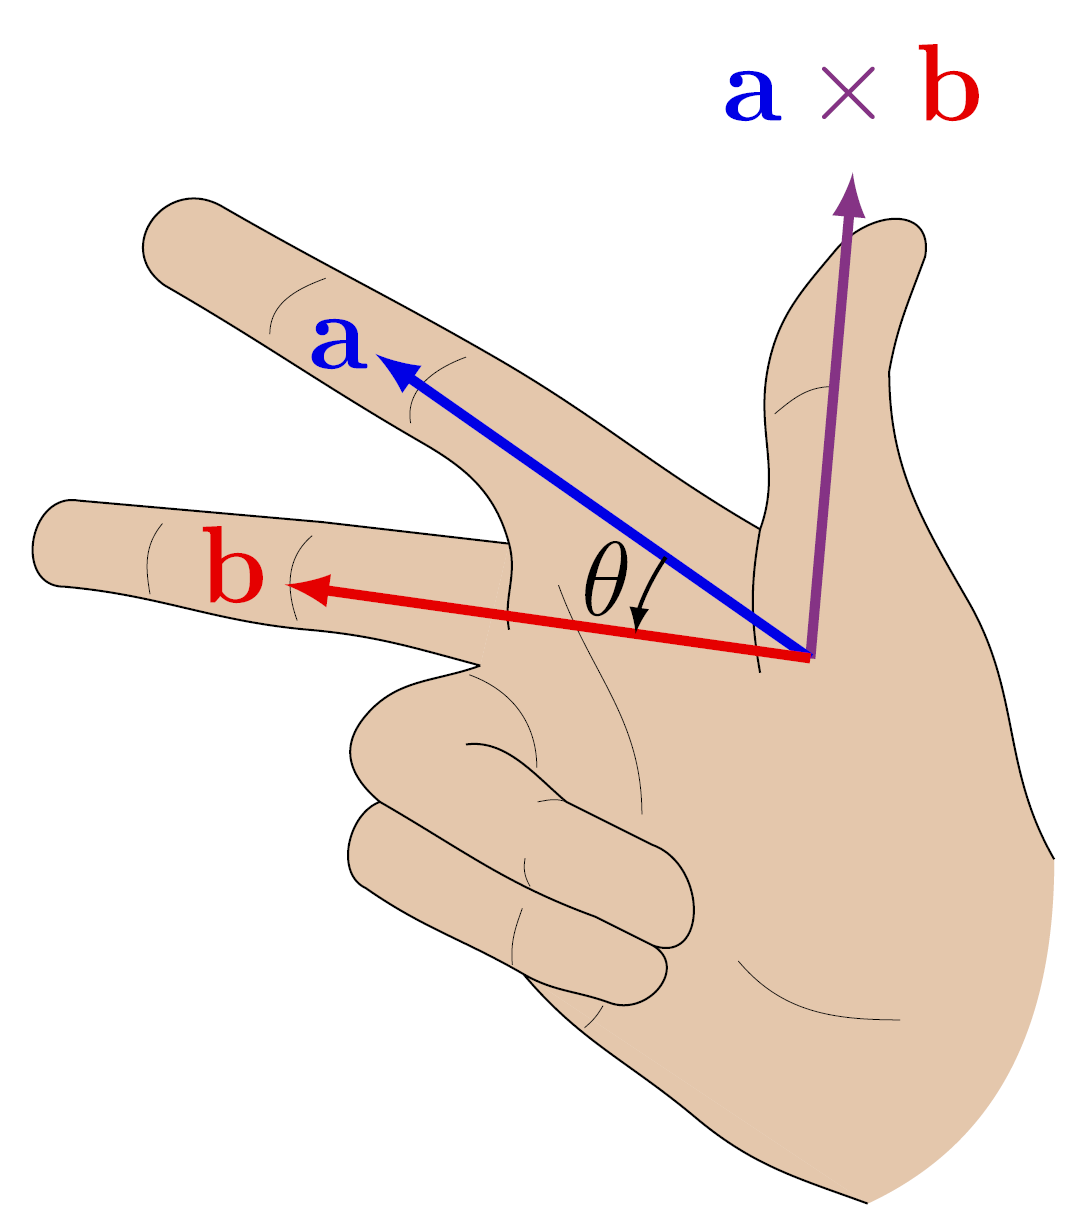
\includegraphics[width=0.15\linewidth]{Contenidos/C0_Repaso/Figuras/RMD1.png}
        \caption{Regla de la mano derecha}
        \label{fig:C0_F01_regla_mano_derecha}
    \end{figure}

    \item[Identidades Vectoriales:] Muy útiles para simplificar ecuaciones de movimiento. El producto triple escalar $\vec{a} \cdot (\vec{b} \times \vec{c})$ representa el volumen del paralelepípedo formado por los vectores. Otra identidad crucial es el doble producto vectorial: $\vec{a} \times (\vec{b} \times \vec{c}) = \vec{b}(\vec{a} \cdot \vec{c}) - \vec{c}(\vec{a} \cdot \vec{b})$.

    \item[Matrices de Rotación:] En $\mathbb{R}^3$, permiten transformar las componentes de un vector entre sistemas de referencia con distinta orientación. Si el sistema $B$ rota respecto al sistema $A$ un ángulo $\theta$ sobre el eje $z$, la matriz de rotación es:
    $$R_{A/B} = \begin{pmatrix} \cos\theta & -\sin\theta & 0 \\ \sin\theta & \cos\theta & 0 \\ 0 & 0 & 1 \end{pmatrix}$$
    Propiedad fundamental: $R^{-1} = R^T$.

    \item[Derivada:] Matemáticamente, es el límite de la razón de cambio de una función respecto a la variación de su variable independiente. Representa la pendiente de la recta tangente a la curva en un punto dado:
    $$f'(x) = \lim_{h \to 0} \frac{f(x+h) - f(x)}{h}$$
    En términos físicos, mide la tasa de variación instantánea de una magnitud.

    \item[Regla de la Cadena:] Es una fórmula para derivar la composición de dos o más funciones. Si $y$ depende de $u$, y $u$ depende de $x$, entonces:
    $$\frac{dy}{dx} = \frac{dy}{du} \cdot \frac{du}{dx}$$
    Es fundamental en dinámica para derivar funciones que dependen implícitamente del tiempo.

    \item[Integral Definida:] Se define como el límite de una suma de áreas de rectángulos (Suma de Riemann) bajo una curva en un intervalo $[a, b]$. Representa la acumulación neta de una cantidad:
    $$\int_{a}^{b} f(x) \, dx = \lim_{n \to \infty} \sum_{i=1}^{n} f(x_i^*) \Delta x$$

    \item[Teorema Fundamental del Cálculo:] Establece la conexión entre la derivación y la integración, indicando que son procesos inversos. Permite calcular integrales mediante la antiderivada $F(x)$:
    $$\int_{a}^{b} f(x) \, dx = F(b) - F(a) \quad \text{donde } F'(x) = f(x)$$

    \item[Gradiente ($\nabla$):] Es un operador vectorial que, aplicado a una función escalar $\phi$, genera un vector cuyas componentes son las derivadas parciales de la función. Indica la dirección de máximo crecimiento de la función:
    $$\nabla \phi = \frac{\partial \phi}{\partial x}\hat{i} + \frac{\partial \phi}{\partial y}\hat{j} + \frac{\partial \phi}{\partial z}\hat{k}$$

    \item[Divergencia ($\nabla \cdot$):] Mide la tendencia de un campo vectorial a originarse o converger en un punto determinado. Es un escalar que resulta del producto punto entre el operador nabla y un vector $\vec{A}$:
    $$\text{div } \vec{A} = \nabla \cdot \vec{A}$$

    \begin{figure}[!ht]
        \centering
        % --- DIVERGENCIA POSITIVA ---
        \tikzset{>=latex}
        \colorlet{veccol}{orange!90!black}
        \colorlet{myblue}{blue!60!black}
        \tikzstyle{vector}=[->,thick,veccol]
        \def\Rad{1.4}
        \def\rad{0.03}
        \def\N{9}

        \begin{tikzpicture}[baseline=(current bounding box.center)]
            \fill[myblue] (0,0) circle (\rad);
            \foreach \i [evaluate={\ang=\i*360/\N;}] in {1,...,\N}{
                \draw[vector] (\ang:0.1*\Rad) --++ (\ang:\Rad);
            }
            \node at (0,-1.5*\Rad) {$\nabla\cdot\vec{v} > 0$};
        \end{tikzpicture}
        \hfill
        % --- DIVERGENCIA NEGATIVA ---
        \begin{tikzpicture}[baseline=(current bounding box.center)]
            \fill[myblue] (0,0) circle (\rad);
            \foreach \i [evaluate={\ang=\i*360/\N;}] in {1,...,\N}{
                \draw[vector] (\ang:1.1*\Rad) -- (\ang:0.1*\Rad);
            }
            \node at (0,-1.5*\Rad) {$\nabla\cdot\vec{v} < 0$};
        \end{tikzpicture}
        \hfill
        % --- DIVERGENCIA CERO ---
        \begin{tikzpicture}[baseline=(current bounding box.center)]
            \foreach \x in {-0.8, 0, 0.8} {
                \foreach \y in {-0.8, 0, 0.8} {
                    \draw[vector] (\x-0.2*\Rad, \y) -- (\x+0.5*\Rad, \y);
                }
            }
            \node at (0,-1.5*\Rad) {$\nabla\cdot\vec{v} = 0$};
        \end{tikzpicture}
        \caption{Representación geométrica de la divergencia}
        \label{fig:C0_F02_divergencia}
    \end{figure}

    \item[Rotor o Rotacional ($\nabla \times$):] Es un operador que mide la tendencia de un campo vectorial a rotar alrededor de un punto. El resultado es un vector:
    $$\text{curl } \vec{A} = \nabla \times \vec{A}$$

    \begin{figure}[!ht]
        \centering
        % --- ROTACIONAL POSITIVO ---
        \tikzset{>=latex}
        \colorlet{veccol}{orange!90!black}
        \colorlet{myblue}{blue!60!black}
        \tikzstyle{vector}=[->,thick,veccol]
        \def\Rad{1.4}
        \def\rad{0.03}
        \def\N{9}

        \begin{tikzpicture}[baseline=(current bounding box.center),scale=0.8]
            \fill[myblue] (0,0) circle (\rad);
            \foreach \i [evaluate={\ang=\i*360/\N;}] in {0,...,\N}{
                \draw[vector] (\ang:\Rad) --++ (\ang+90:0.8*\Rad);
            }
            \node at (0,-1.5*\Rad) {$\nabla\times\vec{v} > 0$};
        \end{tikzpicture}
        \hfill
        % --- ROTACIONAL NEGATIVO ---
        \begin{tikzpicture}[baseline=(current bounding box.center),scale=0.8]
            \fill[myblue] (0,0) circle (\rad);
            \foreach \i [evaluate={\ang=\i*360/\N;}] in {0,...,\N}{
                \draw[vector] (\ang:\Rad) --++ (\ang-90:0.8*\Rad);
            }
            \node at (0,-1.5*\Rad) {$\nabla\times\vec{v} < 0$};
        \end{tikzpicture}
        \hfill
        % --- ROTACIONAL CERO ---
        \begin{tikzpicture}[baseline=(current bounding box.center),scale=0.8]
            \fill[myblue] (0,0) circle (\rad);
            \foreach \i [evaluate={\ang=\i*360/\N;}] in {0,...,\N}{
                \draw[vector] (\ang:0.2*\Rad) -- (\ang:1.2*\Rad);
            }
            \node at (0,-1.5*\Rad) {$\nabla\times\vec{v} = 0$};
        \end{tikzpicture}
        \caption{Rotacional representado mediante vectores tangenciales y radiales}
        \label{fig:C0_F03_rotacional}
    \end{figure}

    \item[Teorema del Transporte:] Sea un vector $\vec{a}$ cualquiera. Su derivada temporal puede ser encontrada como $$\transport{\vec{a}}{A}{B}$$
    
    donde $A$ y $B$ son marcos de referencia.
    Este es un resultado fundamental que conecta las derivadas de un vector en dos sistemas de referencia en rotación relativa.

\end{description}

\newpage

% Incluir secciones teóricas
% =========================================================================
% Capítulo 0 - Sección 1: Álgebra de Vectores
% =========================================================================
\section{Álgebra de Vectores}

Este sección presenta los ejercicios fundamentales de álgebra vectorial,
incluyendo operaciones con bases ortonormales, productos punto y cruz,
e identidades vectoriales clave.

% Incluir ejercicios de Algebra (actualizaremos rutas con cada migración)
\input{Contenidos/Capitulo 0_ Repaso/Ejercicios/Problemas/Algebra/Problema 1}
\input{Contenidos/Capitulo 0_ Repaso/Ejercicios/Problemas/Algebra/Problema 2}
\input{Contenidos/Capitulo 0_ Repaso/Ejercicios/Problemas/Algebra/Problema 3}
\input{Contenidos/Capitulo 0_ Repaso/Ejercicios/Problemas/Algebra/Problema 4}
\input{Contenidos/Capitulo 0_ Repaso/Ejercicios/Problemas/Algebra/Problema 5}
\input{Contenidos/Capitulo 0_ Repaso/Ejercicios/Problemas/Algebra/Problema 6}

\newpage
%% =========================================================================
% Capítulo 0 - Sección 2: Cálculo Vectorial
% =========================================================================
\section{Cálculo Vectorial}

Este sección contiene ejercicios sobre las operaciones de cálculo vectorial:
gradiente, divergencia, rotacional y el teorema del transporte.
Estos conceptos son esenciales para formular las ecuaciones de movimiento.

\subsection{Ejercicios}

\subsection{Problema 1: Derivadas e Integrales Simples}
Resuelva las siguientes operaciones de cálculo básico respecto a una variable $t$ o $x$:

\begin{multicols}{2}
\begin{enumerate}
    \item Halle $\frac{d}{dt} [t^2 \cos(3t)]$.
    \item Halle $\frac{d}{dt} [ \ln(t^2 + 1) e^{-2t} ]$.
    \item Calcule $\int (3t^2 - 5\sin(t)) dt$.
    \item Calcule $\int x e^{x^2} dx$.
    \item Halle $\frac{d}{dt} [ \sqrt{1 + \sin^2(t)} ]$.
    \item Evalúe $\int_0^1 \frac{1}{1+x^2} dx$.
    \item Halle $\frac{d}{dt} [ \arctan(t^2) ]$.
    \item Calcule $\int x^2 \ln(x) dx$.
\end{enumerate}
\end{multicols}
% --- PROBLEMA 2: MULTIVARIABLE (PURO) ---
\subsection{Problema 2: Derivadas Parciales e Integrales Dobles (Cálculo 2)}
Realice los cálculos indicados para funciones de varias variables:

\begin{multicols}{2}
\begin{enumerate}
    \item Sea $f(x,y) = x^3 y^2 + \sin(xy)$, halle $\frac{\partial f}{\partial x}$.
    \item Sea $g(x,y) = e^{x^2+y^2}$, halle $\frac{\partial^2 g}{\partial x \partial y}$.
    \item Evalúe $\int_0^1 \int_0^2 (x + 2y) \, dy \, dx$.
    \item Evalúe $\int_0^\pi \int_0^R r \, dr \, d\theta$.
    \item Halle el gradiente $\nabla \phi$ de $\phi = \sqrt{x^2 + y^2 + z^2}$.
    \item Calcule $\int_0^a \int_0^{a-x} dy \, dx$.
\end{enumerate}
\end{multicols}
% =========================================================================
% Capítulo 0: Repaso
% Tema 02: Cálculo vectorial
% Problema 03: Derivadas de Vectores y Productos
% =========================================================================
\subsubsection{Derivadas de Vectores y Productos}
Considere que $\vec{u}(t)$ y $\vec{v}(t)$ son vectores que dependen del tiempo. Calcule:

\begin{enumerate}
    \item Halle $\frac{d}{dt} (\vec{u} \cdot \vec{v})$.
    \item Halle $\frac{d}{dt} (\vec{u} \times \vec{v})$.
    \item Sea $\vec{r}(t) = \cos(\omega t)\vec{i} + \sin(\omega t)\vec{j} + bt\vec{k}$. Calcule $\dot{\vec{r}}$ y $\ddot{\vec{r}}$.
    \item Si $\vec{v} = \dot{\vec{r}}$, calcule la derivada de la energía cinética escalar: $\frac{d}{dt} (\frac{1}{2} m \vec{v} \cdot \vec{v})$.
\end{enumerate}
% --- SOLUCIÓN ---------------------------------------------------------------
\begin{solucion}{Derivación Vectorial}
\begin{enumerate}
    \item $\frac{d}{dt} (\vec{u} \cdot \vec{v}) = \dot{\vec{u}} \cdot \vec{v} + \vec{u} \cdot \dot{\vec{v}}$.
    \item $\vec{r}(t) = \cos(\omega t)\vec{i} + \sin(\omega t)\vec{j} + bt\vec{k}$. 
    Derivando componente a componente:
    $\dot{\vec{r}} = -\omega\sin(\omega t)\vec{i} + \omega\cos(\omega t)\vec{j} + b\vec{k}$.
    $\ddot{\vec{r}} = -\omega^2\cos(\omega t)\vec{i} - \omega^2\sin(\omega t)\vec{j}$.
    \item $\frac{d}{dt} (\frac{1}{2} m \vec{v} \cdot \vec{v}) = \frac{1}{2} m (\dot{\vec{v}} \cdot \vec{v} + \vec{v} \cdot \dot{\vec{v}}) = m \vec{v} \cdot \dot{\vec{v}} = m \vec{v} \cdot \vec{a} = P$ (Potencia).
\end{enumerate}
\end{solucion}

% --- PROBLEMA 4: BASES INTRÍNSECAS ---
\subsection{Problema 4: Curvas Parametrizadas (Base de Serret-Frenet)}
Para la siguiente curva en el espacio, obtenga los vectores unitarios Tangente ($\hat{T}$), Normal ($\hat{N}$) y Binormal ($\hat{B}$):

$$\vec{r}(s) = \left( a \cos\left(\frac{s}{c}\right), a \sin\left(\frac{s}{c}\right), \frac{b s}{c} \right)$$ 
donde $c = \sqrt{a^2 + b^2}$ y $s$ es el parámetro de longitud de arco.

\begin{enumerate}
    \item Obtenga $\hat{T} = \frac{d\vec{r}}{ds}$.
    \item Obtenga $\hat{N} = \frac{d\hat{T}/ds}{\|d\hat{T}/ds\|}$.
    \item Obtenga $\hat{B} = \hat{T} \times \hat{N}$.
    \item Calcule la curvatura $\kappa = \|\frac{d\hat{T}}{ds}\|$.
\end{enumerate}
% --- PROBLEMA 5: INTEGRALES TRIPLES (APLICADO) ---
\subsection{Problema 5: Distribución de Masa y Volúmenes}
Calcule las siguientes integrales triples sobre los volúmenes indicados (asuma densidad $\rho$ constante):

\begin{enumerate}
    \item Calcule la integral $J = \rho \iiint_V (x^2 + y^2) \, dV$ para un cilindro de radio $R$ y altura $H$ centrado en el eje $z$.
    \item Calcule la integral $P_{xy} = \rho \iiint_V (xy) \, dV$ para un cubo de lado $L$ en el primer octante ($0 \le x,y,z \le L$).
    \item Evalúe $I_0 = \rho \iiint_V (x^2 + y^2 + z^2) \, dV$ para una esfera de radio $R$.
    \item Calcule el volumen de un sólido definido por $x^2 + y^2 \le z \le H$.
\end{enumerate}
% =========================================================================
% Capítulo 0: Repaso
% Tema 02: Cálculo vectorial
% Problema 06: Centros de Masa
% =========================================================================
\subsubsection{Centros de Masa}
El centro de masa ($\vec{r}_{cm}$) representa el punto donde se puede considerar concentrada toda la masa de un sistema.

\begin{enumerate}
    \item Sistema de Partículas: Se tienen tres masas puntuales: $m_1 = 2$ kg en $(1, 0, 0)$, $m_2 = 3$ kg en $(0, 2, 0)$ y $m_3 = 5$ kg en $(0, 0, 2)$. Halle la posición del centro de masa $\vec{r}_{cm}$.
    \item Lámina Semicircular: Calcule la coordenada $\bar{y}$ del centro de masa de una placa plana semicircular de radio $R$ y densidad constante $\rho$, situada en el plano $xy$ sobre el eje $x$ (con el diámetro sobre el eje $x$).
    \item Barra no uniforme: Una barra de longitud $L$ tiene una densidad lineal $\lambda(x) = kx$. Halle la posición $\bar{x}$ de su centro de masa.
\end{enumerate}
% --- SOLUCIÓN ---------------------------------------------------------------
\begin{solucion}{Centro de Masa}
\begin{enumerate}
    \item $\vec{r}_{cm} = \frac{\sum m_i \vec{r}_i}{\sum m_i} = \frac{2(1,0,0) + 3(0,2,0) + 5(0,0,2)}{2+3+5} = \frac{(2, 6, 10)}{10} = (0.2, 0.6, 1.0)$.
    \item $\bar{y} = \frac{1}{M} \iint y \rho dA$. En polares: $y = r\sin\theta$, $dA = r \, dr \, d\theta$.
    $M = \frac{1}{2}\pi R^2 \rho$. 
    $\iint y \rho dA = \rho \int_0^\pi \int_0^R r^2 \sin\theta \, dr \, d\theta = \rho \frac{R^3}{3} [-\cos\theta]_0^\pi = \frac{2\rho R^3}{3}$.
    $\bar{y} = \frac{2\rho R^3 / 3}{\pi R^2 \rho / 2} = \frac{4R}{3\pi}$.
    \item $M = \int_0^L kx \, dx = \frac{1}{2}kL^2$. 
    $\bar{x} = \frac{1}{M} \int_0^L x (kx) dx = \frac{1}{M} \frac{kL^3}{3} = \frac{kL^3/3}{kL^2/2} = \frac{2}{3}L$.
\end{enumerate}
\end{solucion}


\newpage
\subsection{Soluciones}

\subsection{Solucionario: Cálculo}

% ---  1 ---
\begin{sol}[{Cálculo Unidimensional}]
\begin{enumerate}
    \item $\frac{d}{dt} [t^2 \cos(3t)]$: Usando la regla del producto $(uv)' = u'v + uv'$:
    $2t \cos(3t) + t^2 (-\sin(3t) \cdot 3) = 2t\cos(3t) - 3t^2\sin(3t)$.
    
    \item $\frac{d}{dt} [ \ln(t^2 + 1) e^{-2t} ]$: Regla del producto y cadena:
    $\frac{2t}{t^2+1} e^{-2t} + \ln(t^2+1) (-2e^{-2t}) = e^{-2t} \left( \frac{2t}{t^2+1} - 2\ln(t^2+1) \right)$.
    
    \item $\int (3t^2 - 5\sin(t)) dt$: Integración directa:
    $t^3 - 5(-\cos(t)) + C = t^3 + 5\cos(t) + C$.
    
    \item $\int x e^{x^2} dx$: Sustitución $u = x^2$, $du = 2x dx$:
    $\frac{1}{2} \int e^u du = \frac{1}{2} e^{x^2} + C$.
\end{enumerate}
\end{sol}

% ---  2 ---
\begin{sol}[{ Cálculo Multivariable}]
\begin{enumerate}
    \item $\frac{\partial}{\partial x}(x^3 y^2 + \sin(xy))$: Se trata a $y$ como constante:
    $3x^2 y^2 + \cos(xy) \cdot y = 3x^2 y^2 + y\cos(xy)$.
    
    \item $\frac{\partial^2}{\partial x \partial y} (e^{x^2+y^2})$: Primero derivamos respecto a $y$: $\frac{\partial}{\partial y} = 2y e^{x^2+y^2}$. Luego respecto a $x$: $2y (e^{x^2+y^2} \cdot 2x) = 4xy e^{x^2+y^2}$.
    
    \item $\int_0^1 \int_0^2 (x + 2y) \, dy \, dx$: 
    $\int_0^1 [xy + y^2]_0^2 dx = \int_0^1 (2x + 4) dx = [x^2 + 4x]_0^1 = 1 + 4 = 5$.
    
    \item $\int_0^\pi \int_0^R r \, dr \, d\theta$: 
    $\int_0^\pi [\frac{r^2}{2}]_0^R d\theta = \frac{R^2}{2} \int_0^\pi d\theta = \frac{\pi R^2}{2}$.
\end{enumerate}
\end{sol}

% ---  3 ---
\begin{sol}[{ Derivación Vectorial}]
\begin{enumerate}
    \item $\frac{d}{dt} (\vec{u} \cdot \vec{v}) = \dot{\vec{u}} \cdot \vec{v} + \vec{u} \cdot \dot{\vec{v}}$.
    \item $\vec{r}(t) = \cos(\omega t)\vec{i} + \sin(\omega t)\vec{j} + bt\vec{k}$. 
    Derivando componente a componente:
    $\dot{\vec{r}} = -\omega\sin(\omega t)\vec{i} + \omega\cos(\omega t)\vec{j} + b\vec{k}$.
    $\ddot{\vec{r}} = -\omega^2\cos(\omega t)\vec{i} - \omega^2\sin(\omega t)\vec{j}$.
    \item $\frac{d}{dt} (\frac{1}{2} m \vec{v} \cdot \vec{v}) = \frac{1}{2} m (\dot{\vec{v}} \cdot \vec{v} + \vec{v} \cdot \dot{\vec{v}}) = m \vec{v} \cdot \dot{\vec{v}} = m \vec{v} \cdot \vec{a} = P$ (Potencia).
\end{enumerate}
\end{sol}

% ---  4 ---
\begin{sol}[{ Bases Intrínsecas}]
Para $\vec{r}(s) = \left( a \cos(\frac{s}{c}), a \sin(\frac{s}{c}), \frac{bs}{c} \right)$ con $c = \sqrt{a^2+b^2}$:
\begin{enumerate}
    \item $\hat{T} = \frac{d\vec{r}}{ds} = \frac{1}{c} \left( -a\sin(\frac{s}{c}), a\cos(\frac{s}{c}), b \right)$.
    \item $\frac{d\hat{T}}{ds} = \frac{1}{c^2} (-a\cos(\frac{s}{c}), -a\sin(\frac{s}{c}), 0)$. La norma es $\frac{a}{c^2}$.
    $\hat{N} = \frac{d\hat{T}/ds}{a/c^2} = (-\cos(\frac{s}{c}), -\sin(\frac{s}{c}), 0)$.
    \item $\hat{B} = \hat{T} \times \hat{N} = \frac{1}{c} (b\sin(\frac{s}{c}), -b\cos(\frac{s}{c}), a)$.
\end{enumerate}
\end{sol}

% ---  5 ---
\begin{sol}[{ Integrales Triples}]
\begin{enumerate}
    \item $J = \rho \int_0^H \int_0^{2\pi} \int_0^R r^2 (r \, dr \, d\theta \, dz)$: 
    $J = \rho \cdot H \cdot 2\pi \cdot \frac{R^4}{4} = \frac{1}{2} (\rho \pi R^2 H) R^2 = \frac{1}{2} M R^2$.
    \item $P_{xy} = \rho \int_0^L x \, dx \int_0^L y \, dy \int_0^L dz = \rho (\frac{L^2}{2})(\frac{L^2}{2})(L) = \frac{1}{4} \rho L^5 = \frac{1}{4} ML^2$.
\end{enumerate}
\end{sol}

% ---  6 ---
\begin{sol}[{ Centro de Masa}]
\begin{enumerate}
    \item $\vec{r}_{cm} = \frac{\sum m_i \vec{r}_i}{\sum m_i} = \frac{2(1,0,0) + 3(0,2,0) + 5(0,0,2)}{2+3+5} = \frac{(2, 6, 10)}{10} = (0.2, 0.6, 1.0)$.
    \item $\bar{y} = \frac{1}{M} \iint y \rho dA$. En polares: $y = r\sin\theta$, $dA = r \, dr \, d\theta$.
    $M = \frac{1}{2}\pi R^2 \rho$. 
    $\iint y \rho dA = \rho \int_0^\pi \int_0^R r^2 \sin\theta \, dr \, d\theta = \rho \frac{R^3}{3} [-\cos\theta]_0^\pi = \frac{2\rho R^3}{3}$.
    $\bar{y} = \frac{2\rho R^3 / 3}{\pi R^2 \rho / 2} = \frac{4R}{3\pi}$.
    \item $M = \int_0^L kx \, dx = \frac{1}{2}kL^2$. 
    $\bar{x} = \frac{1}{M} \int_0^L x (kx) dx = \frac{1}{M} \frac{kL^3}{3} = \frac{kL^3/3}{kL^2/2} = \frac{2}{3}L$.
\end{enumerate}
\end{sol}


\newpage

% Capítulo 1: Cinemática
%% =========================================================================
% Capítulo 1: Cinemática
% =========================================================================
% Archivo: C1_00_introduccion.tex
% Descripción: Movimiento de puntos y sistemas de referencias
% =========================================================================

\chapter{Cinemática}

\section*{Introducción}

La cinemática es la rama de la mecánica que describe el movimiento sin considerar las causas que lo producen (fuerzas). En este capítulo estudiaremos cómo representar la posición, velocidad y aceleración de puntos materiales en diferentes sistemas de coordenadas, y cómo derivar vectores expresados en marcos de referencia que se mueven o rotan entre sí. La herramienta central será el Teorema del Transporte, que usaremos de manera sistemática en todos los problemas del libro.

\subsection*{Sistemas de Coordenadas}

El análisis cinemático depende críticamente de la elección del sistema de coordenadas. En este libro estudiaremos:

\begin{enumerate}
    \item \textbf{Coordenadas Cartesianas}: El sistema más simple e intuitivo.
    \item \textbf{Coordenadas Cilíndricas}: Naturales para problemas con simetría axial.
    \item \textbf{Coordenadas Esféricas}: Útiles para sistemas con simetría central.
    \item \textbf{Coordenadas Intrínsecas}: Basadas en la geometría de la trayectoria.
\end{enumerate}

La Figura \ref{fig:c1_intro_coordenadas_esfericas} muestra el sistema de coordenadas esféricas con sus vectores unitarios $\{\hat{e}_r, \hat{e}_\theta, \hat{e}_\phi\}$, que junto con las coordenadas cilíndricas será uno de los sistemas más usados en los problemas de este capítulo.

% =========================================================================
% Figura: Sistema de coordenadas esféricas
% =========================================================================
% Archivo: Coordenadas_esfericas.tikz.tex
% Usada en: C1_00_introduccion.tex
% Convención del libro: theta = ángulo azimutal (plano xy), phi = ángulo polar
% =========================================================================

\begin{figure}[!ht]
    \centering
    \tdplotsetmaincoords{70}{110}
    \begin{tikzpicture}[tdplot_main_coords, >=Latex,
                        ejes/.style={->, thick, gris1},
                        univec/.style={->, very thick, azul},
                        posvec/.style={->, very thick, myred}]

        % --- CONFIGURACIÓN DE PARÁMETROS ---
        \pgfmathsetmacro{\phivec}{48.17}   % Ángulo polar [deg]
        \pgfmathsetmacro{\thetavec}{63.5}  % Ángulo azimutal [deg]
        \def\rlen{6}                       % Largo del vector posición [u]

        % --- SISTEMAS DE COORDENADAS ---
        \draw[ejes] (0,0,0) -- (6.5,0,0) node[pos=1.1] {$x$};
        \draw[ejes] (0,0,0) -- (0,6,0) node[pos=1.05] {$y$};
        \draw[ejes] (0,0,0) -- (0,0,5.5) node[pos=1.05] {$z$};

        % --- PUNTOS Y COORDENADAS ---
        \tdplotsetcoord{P}{\rlen}{\phivec}{\thetavec}

        % --- VECTORES Y FUERZAS ---
        % Vector posición
        \draw[posvec] (0,0,0) -- (P) node[midway, above left] {$\vec{r}$};
        % Vectores unitarios en el punto P
        \tdplotsetcoord{Er}{7}{\phivec}{\thetavec}
        \draw[univec] (0,0,0) -- (Er) node[pos=1.05] {$\hat{e}_r$};
        \tdplotsetcoord{Et}{1}{90}{90+\thetavec}
        \draw[univec] (Pxy) -- ($(Et) + (Pxy)$) node[pos=1.3] {$\hat{e}_\theta$};
        \tdplotsetcoord{Ep}{1}{90+\phivec}{\thetavec}
        \draw[univec] (P) -- ($(Ep) + (P)$) node[pos=1.3] {$\hat{e}_\phi$};

        % --- ANOTACIONES Y ETIQUETAS ---
        % Líneas de ayuda (proyecciones)
        \draw[thick] (0,0,0) -- (Pxy);
        \draw[mydashed, gris1!60] (P) -- (Pxy);
        \draw[mydashed, gris1!60] (Px) -- (Pxy) node[pos=-0.15] {$x$};
        \draw[mydashed, gris1!60] (Py) -- (Pxy) node[pos=-0.3] {$y$};
        \draw[mydashed, gris1!60] (Pz) -- (P) node[pos=-0.15] {$z$};
        % Punto P
        \node[fill=gris1, circle, inner sep=0.9pt, label={above right:$P$}] at (P) {};
        % Ángulos
        \tdplotdrawarc{(0,0,0)}{0.7}{0}{\thetavec}{below}{$\theta$}
        \tdplotsetthetaplanecoords{\thetavec}
        \tdplotdrawarc[tdplot_rotated_coords]{(0,0,0)}{0.5}{0}{\phivec}{}{}
        \node at (0,0.25,0.67) {$\phi$};

    \end{tikzpicture}
    \caption{Coordenadas esféricas y sus vectores unitarios en el punto $P$}
    \label{fig:c1_intro_coordenadas_esfericas}
\end{figure}


\subsection*{Marcos de Referencia}

Un concepto fundamental es la distinción entre:
\begin{description}
    \item[Marcos Inerciales:] Sistemas de referencia en los que las leyes de Newton se cumplen sin términos de corrección.
    \item[Marcos No-Inerciales:] Sistemas acelerados o en rotación donde aparecen fuerzas ficticias.
\end{description}

\subsection*{Derivadas en Marcos Móviles}

El \textbf{Teorema del Transporte} permite relacionar las derivadas de un vector en dos marcos de referencia que rotan uno respecto al otro:

\[\transport{\vec{a}}{A}{B}\]

donde $\mathcal{A}$ es el marco fijo (inercial), $\mathcal{B}$ es el marco móvil y $\velang{A}{B}$ es la velocidad angular del marco $\mathcal{B}$ respecto al marco $\mathcal{A}$. Esta es la misma notación que usaremos en las soluciones de los problemas.

\section{Conceptos Clave de Cinemática}

\begin{description}

    \item[Posición:] Vector $\vec{r}(t)$ que especifica la ubicación de un punto.

    \item[Velocidad:] Primera derivada de la posición,
    $$\vec{v}(t) = \frac{d\vec{r}}{dt}$$
    Representa la tasa de cambio de posición.

    \item[Aceleración:] Segunda derivada de la posición (primera de la velocidad),
    $$\vec{a}(t) = \frac{d\vec{v}}{dt} = \frac{d^2\vec{r}}{dt^2}$$
    Representa la tasa de cambio de velocidad.

    \item[Velocidad Angular:] Para marcos móviles, $\vec{\omega}$ describe la rotación.

    \item[Aceleración Angular:] Primera derivada de la velocidad angular,
    $$\vec{\alpha} = \frac{d\vec{\omega}}{dt}$$

    \item[Velocidad Relativa:] En sistemas con dos marcos de referencia,
    $$\vec{v}_{P/B} = \vec{v}_P - \vec{v}_B$$

    \item[Composición de Velocidades:] Relaciona velocidades en marcos diferentes,
    $$\vec{v}_{P/A} = \vec{v}_{P/B} + \vec{v}_{B/A}$$

    \item[Restricciones:] Condiciones que relacionan las variables del sistema.
    Ejemplos: movimiento en una curva, rodadura sin deslizar, etc.

\end{description}

\section*{Objetivos del Capítulo}

Al completar este capítulo, deberás:
\begin{itemize}
    \item Usar competentemente los cuatro sistemas de coordenadas principales.
    \item Calcular velocidad y aceleración en cada sistema.
    \item Aplicar el Teorema del Transporte para marcos móviles.
    \item Analizar movimientos complejos usando cambios de marco.
    \item Resolver problemas con restricciones de movimiento.
\end{itemize}

\newpage

%\newpage
% =========================================================================
% Capítulo 1 - Tema 01: Cinemática en Coordenadas Cilíndricas
% =========================================================================

\section{Tema 01: Cinemática en Coordenadas Cilíndricas}

En este tema estudiamos el movimiento de puntos expresado en coordenadas cilíndricas.
Este sistema es natural para problemas con simetría axial o movimiento rotacional.

\subsection{Ejercicios}

\subsubsection{Hormiga velocista}
En la figura \ref{fig:Hormiga}, se encuentra una hormiga (Punto $B$), la cual camina de manera radial, hacia afuera del disco a una velocidad constante $v_0$ desde el centro. Si el disco rota desde su centro $O$ con una velocidad angular de magnitud $\Omega$ relativa al suelo, determine:
\begin{enumerate}
    \item La posición con respecto al tiempo.
    \item La velocidad con respecto al tiempo.
    \item La aceleración con respecto al tiempo.
\end{enumerate}

\begin{figure}[!ht]
    \centering
\begin{tikzpicture}[>=Latex, scale=1.5]

    % --- CONFIGURACIÓN DE DIMENSIONES ---
    \def\R{3}      % Radio mayor de la elipse (ancho)
    \def\r{0.8}    % Radio menor de la elipse (alto/perspectiva)
    \def\h{0.15}   % Grosor del disco
    \def\Hshaft{1.2} % Largo del eje

    % 1. EJE CENTRAL (PARTE INFERIOR)
    % Dibujamos el cilindro del eje debajo del disco
    \fill[gray!60] (-0.4, -\h) rectangle (0.4, -\Hshaft);
    \draw[thick] (-0.4, -\h) -- (-0.4, -\Hshaft);
    \draw[thick] (0.4, -\h) -- (0.4, -\Hshaft);
    \draw[thick, fill=gray!70] (0, -\Hshaft) ellipse (0.4 and 0.15);

    % 2. GROSOR DEL DISCO (BORDE LATERAL)
    % Se dibuja la mitad inferior de la elipse desplazada hacia abajo
    \fill[gray!50] (\R, 0) arc (0:-180:\R\space and \r) -- (-\R, -\h) arc (-180:0:\R\space and \r) -- cycle;
    \draw[thick] (\R, 0) arc (0:-180:\R\space and \r);
    \draw[thick] (\R, -\h) arc (0:-180:\R\space and \r);
    \draw[thick] (\R, 0) -- (\R, -\h);
    \draw[thick] (-\R, 0) -- (-\R, -\h);

    % 3. SUPERFICIE SUPERIOR DEL DISCO
    \draw[thick, fill=gray!20] (0,0) ellipse [x radius=\R, y radius=\r];

    % 4. PUNTOS Y VECTORES
    % Punto O (Centro)
    \coordinate (O) at (0,0);
    \filldraw (O) circle (1.5pt) node[left, xshift=-2pt] {$O$};

    % Punto B (Partícula) - Calculado para que parezca estar sobre la elipse
    % Usamos coordenadas polares modificadas por la proporción de la elipse
    \def\ang{20} % Ángulo de posición
    \def\dist{2.0} % Distancia radial r
    \coordinate (B) at ({\dist*cos(\ang)}, {\dist*sin(\ang)*(\r/\R)});

    % Dibujo del grupo de puntos B
    \filldraw (B) circle (1.5pt);

    \node[below right] at (B) {$B$};

    % Vector r (Posición)
    \draw[->, thick] (O) -- (B) node[midway, above] {$r$};

    % Vector v0 (Velocidad tangencial)
    % El ángulo de v0 debe seguir la inclinación de la elipse (tangente)
    \draw[->, very thick, blue] (B) -- ++({0.8*cos(\ang)}, {0.8*sin(\ang)*(\r/\R)}) node[below] {$v_0$};

    % 5. INDICADOR DE ROTACIÓN OMEGA
    \draw[->, thick] (-0.6, 0) arc (170:370:0.6 and 0.2);
    \node[left] at (-0.7, -0) {$\Omega$};

\end{tikzpicture}
    \caption{Hormiga Velocista}
    \label{fig:Hormiga}
\end{figure}
\subsubsection{Movimiento en coordenadas cilíndricas}

Se observa una partícula en movimiento con respecto a un sistema de referencia inercial. La trayectoria está dada por las siguientes funciones:
\[ r = Ae^{k\theta}, \quad z = hr \]
donde $r, \theta$ y $z$ son coordenadas cilíndricas, siendo $A, k$ y $h$ valores escalares constantes y mayores que cero, como se muestra en la Figura \ref{fig:c1_e01_p02_espiral_cilindricas}. Suponiendo que su rapidez es constante ($v_0$) y conocida:

\begin{enumerate}
    \item Calcule la velocidad $\vec{v}$ de la partícula en función de $\theta, A, k, h$ y $v_0$.
    \item Encuentre su aceleración $\vec{a}$ en función de los mismos parámetros.
    \item Pruebe que $\vec{a} \perp \vec{v}$.
    \item Encuentre una expresión para $\theta(t)$.
\end{enumerate}

% Figura principal
\begin{figure}[!ht]
    \centering
    \begin{tikzpicture}[>=Latex, scale=1.5]

        % --- CONFIGURACIÓN DE PARÁMETROS ---
        \def\A{0.15}      % Constante A de la espiral [u]
        \def\k{0.22}      % Constante k (crecimiento) [-]
        \def\thP{560}     % Ángulo del punto P [deg] (una vuelta y media)
        \def\thPmod{200}  % Azimut equivalente de P [deg]

        % --- SISTEMAS DE COORDENADAS ---
        \draw[->, thick, gris1] (-2.2,0) -- (2.4,0) node[below right] {$x$};
        \draw[->, thick, gris1] (0,-1.8) -- (0,2.2) node[left] {$y$};

        % --- GEOMETRÍA PRINCIPAL ---
        % Espiral logarítmica r = A e^{k theta} (vista superior)
        \draw[thick, gris1, domain=0:720, samples=300, smooth, variable=\t]
            plot ({\t}:{\A*exp(\k*\t/57.29578)});

        % --- PUNTOS Y COORDENADAS ---
        \pgfmathsetmacro{\rP}{\A*exp(\k*\thP/57.29578)}
        \coordinate (O) at (0,0);
        \coordinate (P) at (\thP:\rP);
        \draw[mydashed, gris1!60] (O) -- (P);

        % --- VECTORES Y FUERZAS ---
        % Vectores unitarios cilíndricos en P
        \draw[->, very thick, myred] (P) -- ++(\thP:0.55) node[above left] {$\hat{e}_r$};
        \draw[->, very thick, myred] (P) -- ++(\thP+90:0.55) node[below left] {$\hat{e}_\theta$};
        % Velocidad (tangente a la espiral, rapidez constante v0)
        \pgfmathsetmacro{\alphat}{atan(1/\k)}
        \draw[->, very thick, azul] (P) -- ++(\thP+\alphat:0.9) node[below] {$\vec{v}$};

        % --- ANOTACIONES Y ETIQUETAS ---
        \fill[gris1] (P) circle (1.2pt) node[above right, xshift=1pt] {$P$};
        \node[below left] at (O) {$O$};
        \draw[->] (0.35,0) arc (0:\thPmod:0.35);
        \node at ({\thPmod/2}:0.55) {$\theta$};
        \node[gris1] at (1.6,-1.4) {$r = Ae^{k\theta}$};

    \end{tikzpicture}
    \caption{Vista superior de la espiral $r=Ae^{k\theta}$; la altura crece como $z=hr$}
    \label{fig:c1_e01_p02_espiral_cilindricas}
\end{figure}


\subsubsection{Sistema de doble varilla}
Dos varillas rígidas de longitudes $l_1$ y $l_2$ están articuladas en serie como se muestra en la Figura \ref{fig:doble_varilla}. La varilla $OA$ está articulada en uno de sus extremos al punto fijo $O$, mientras que su otro extremo está articulado en el punto $A$, que es un extremo de la segunda varilla $AP$. El punto $P$ se encuentra en el extremo libre de la varilla $AP$. Sabiendo que $\theta$ es el ángulo entre la varilla $OA$ y la horizontal y que $\phi$ es el ángulo entre la varilla $AP$ y la prolongación de la varilla $OA$, determine:

\begin{enumerate}
    \item La velocidad y aceleración del punto $P$ vistas por un observador fijo a la varilla $OA$.
    \item La velocidad y aceleración del punto $P$ vistas por un observador fijo al suelo.
\end{enumerate}

\begin{figure}[htbp]
    \centering
    \begin{tikzpicture}[>=Latex, scale=1.5]
        % --- Parámetros Geométricos ---
        \def\Lone{2.8}     % Longitud l1
        \def\Ltwo{2.0}     % Longitud l2
        \def\ThetaAng{25}  % Ángulo theta
        \def\PhiAng{35}    % Ángulo phi relativo a OA

        % --- 1. Soporte y Suelo en O ---
        \coordinate (O) at (0,0);
        \draw[thick] (-0.4,-0.4) -- (0.4,-0.4);
        \fill[pattern=north east lines] (-0.4,-0.5) rectangle (0.4,-0.4);
        \draw (O) -- (-0.2,-0.4);
        \draw (O) -- (0.2,-0.4);
        \filldraw[fill=white] (O) circle (2.5pt) node[left, xshift=-2pt] {$O$};

        % --- 2. Varilla OA ---
        \coordinate (A) at ({\ThetaAng}:\Lone);
        % Dibujo de la varilla con estilo 2D
        \draw[line width=5pt, color=gray!20, line cap=round] (O) -- (A);
        \draw[thick] (O) -- (A);
        \filldraw[fill=white] (A) circle (2pt) node[below right] {$A$};
        \node[above left] at ($(O)!0.5!(A)$) {$l_1$};

        % --- 3. Varilla AP ---
        % El ángulo absoluto de AP es (Theta + Phi)
        \coordinate (P) at ($(A) + ({\ThetaAng + \PhiAng}:\Ltwo)$);
        \draw[line width=5pt, color=gray!20, line cap=round] (A) -- (P);
        \draw[thick] (A) -- (P);
        \filldraw (P) circle (1.5pt) node[above right] {$P$};
        \node[above left] at ($(A)!0.5!(P)$) {$l_2$};

        % --- 4. Ángulos y Referencias ---
        % Ángulo theta
        \draw[dashed] (O) -- (1.5,0);
        \draw[->] (0.8,0) arc (0:\ThetaAng:0.8);
        \node at (1.0, 0.2) {$\theta$};

        % Ángulo phi (respecto a la prolongación de OA)
        \coordinate (Prolong) at ($(A) + ({\ThetaAng}:1.2)$);
        \draw[dashed] (A) -- (Prolong);
        \draw[->] ($(A) + ({\ThetaAng}:0.7)$) arc (\ThetaAng:{\ThetaAng+\PhiAng}:0.7);
        \node at ($(A) + ({\ThetaAng + 0.5*\PhiAng}:0.95)$) {$\phi$};

    \end{tikzpicture}
    \caption{Sistema de doble varilla articulada con longitudes $l_1$ y $l_2$, donde se definen los ángulos $\theta$ y $\phi$ para el análisis cinemático.}
    \label{fig:doble_varilla}
\end{figure}
\subsubsection{Collarín en brazo rotatorio}
Un collarín se desliza libremente a lo largo de un brazo rígido, como se muestra en la Figura \ref{fig:collarin_brazo}. El brazo está articulado en uno de sus extremos a un punto $O$, el cual está fijo al suelo, y rota alrededor de una dirección que es ortogonal al plano de movimiento.

Sabiendo que la posición del collarín está descrita por las variables $r$ y $\theta$, donde $r$ es el desplazamiento del collarín relativo al punto $O$ y $\theta$ es el ángulo de la barra medido con respecto a una dirección fija al suelo, determine lo siguiente para un observador fijo al suelo:

\begin{enumerate}
    \item El vector velocidad del collarín.
    \item El vector aceleración del collarín.
    \item La aceleración angular del collarín.
\end{enumerate}

\begin{figure}[!ht]
    \centering
    \begin{tikzpicture}[>=Latex, scale=1.5]
        \def\ang{35} \def\rPos{3.0}
        \coordinate (O) at (0,0);
        \fill[pattern=north east lines] (-0.5,-0.5) rectangle (0.5,-0.4);
        \draw[thick] (-0.5,-0.4) -- (0.5,-0.4);
        \draw (O) -- (-0.25,-0.4);
        \draw (O) -- (0.25,-0.4);
        \filldraw[fill=white] (O) circle (3pt) node[above left] {$O$};
        \coordinate (End) at (\ang:4.5);
        \draw[line width=7pt, color=black,cap=round] (O) -- (End);
        \draw[line width=6pt, color=gray!20,cap=round] (O) -- (End);
        \draw[thick] (O) -- (End);
        
        % COLLARÍN CON DEGRADADO CORREGIDO
        \coordinate (P) at (\ang:\rPos);
        \node[
            top color=gray!5, 
            bottom color=gray!60, 
            draw=black, 
            thick, 
            shape=rounded rectangle, 
            minimum width=0.6cm, 
            minimum height=0.35cm, 
            rotate=\ang+90, 
            inner sep=0pt
        ] at (P) {};
        \filldraw (P) circle (1.2pt) node[above, yshift=6pt] {$P$};

        \draw[dashed] (O) -- (2,0);
        \draw[->] (1,0) arc (0:\ang:1) node[midway, right, xshift=2pt] {$\theta$};
        \draw[|->] ($(O)+(90+\ang:0.4)$) -- ($(P)+(90+\ang:0.4)$) node[midway, above left] {$r$};
        \filldraw[fill=black] (O) circle (1pt);
    \end{tikzpicture}
    \caption{Collarín deslizando sobre un brazo rotatorio.}
    \label{fig:collarin_brazo}
\end{figure}
\ifmostrarSolucion
\begin{tcolorbox}[title= SOlucion Collarian brazo rotatorio, breakable]
\noindent\textbf{Primero, definimos los marcos de referencia y sistemas de coordenadas:}

\vspace{0.3cm}

\noindent $\mathcal{F}$: Suelo (Inercial) \quad $\{\vec{E}_x, \vec{E}_y, \vec{E}_z\}$ \\
\noindent $\mathcal{A}$: Fijo en el brazo \quad $\{\vec{e}_r, \vec{e}_\theta, \vec{e}_z\}$

\vspace{0.5cm}

% --- DIAGRAMA TIKZ Y RELACIONES DE TRANSFORMACIÓN ---
\noindent
\begin{minipage}{0.55\textwidth}
\centering
\begin{tikzpicture}[scale=1.2, >=stealth]
   \def\ang{35} \def\rPos{3.0}
        \coordinate (O) at (0,0);
        \fill[pattern=north east lines] (-0.5,-0.5) rectangle (0.5,-0.4);
        \draw[thick] (-0.5,-0.4) -- (0.5,-0.4);
        \draw (O) -- (-0.25,-0.4);
        \draw (O) -- (0.25,-0.4);
        \filldraw[fill=white] (O) circle (3pt) node[above left] {$O$};
        \coordinate (End) at (\ang:4.5);
        \draw[line width=7pt, color=black,cap=round] (O) -- (End);
        \draw[line width=6pt, color=gray!20,cap=round] (O) -- (End);
        \draw[thick] (O) -- (End);
        
        % COLLARÍN CON DEGRADADO CORREGIDO
        \coordinate (P) at (\ang:\rPos);
        \node[
            top color=gray!5, 
            bottom color=gray!60, 
            draw=black, 
            thick, 
            shape=rounded rectangle, 
            minimum width=0.6cm, 
            minimum height=0.35cm, 
            rotate=\ang+90, 
            inner sep=0pt
        ] at (P) {};
        \filldraw (P) circle (1.2pt) node[above, yshift=6pt] {$P$};

        \draw[dashed] (O) -- (2,0);
        \draw[->] (1,0) arc (0:\ang:1) node[midway, right, xshift=2pt] {$\theta$};
        \draw[|->] ($(O)+(90+\ang:0.4)$) -- ($(P)+(90+\ang:0.4)$) node[midway, above left] {$r$};
        \filldraw[fill=black] (O) circle (1pt);

  % Marco Inercial F (Morado)
  \draw[->, line width=1.2pt, violet] (0,0) -- (2.5,0) node[right] {$\vec{E}_x$};
  \draw[->, line width=1.2pt, violet] (0,0) -- (0,2.5) node[above] {$\vec{E}_y$};
  \node[violet] at (-0.25,0.15) {$\vec{E}_z$};

  % Vector unitario e_theta (Verde)
  \draw[->, line width=1.2pt, green!60!black] (0,0) -- ({2.0*cos(\ang)},{2.0*sin(\ang)}) node[above left] {$\vec{e}_r$};
  \draw[->, line width=1.2pt, green!60!black] (0,0) -- ({2.0*cos(\ang+90)},{2.0*sin(\ang+90)}) node[above left] {$\vec{e}_\theta$};
  \node[green!60!black] at (-0.35,-0.1) {$\vec{e}_z$};
\end{tikzpicture}
\end{minipage}
\begin{minipage}{0.42\textwidth}
\[
\begin{aligned}
\vec{e}_r &= \cos\theta \vec{E}_x + \sin\theta \vec{E}_y \\
\vec{e}_\theta &= -\sin\theta \vec{E}_x + \cos\theta \vec{E}_y \\
\vec{e}_z &= \vec{E}_z
\end{aligned}
\]
\end{minipage}

\vspace{0.8cm}

% --- PARTE A ---
\noindent\textbf{A) Definamos:} 
\[
\vec{r} = r\vec{e}_r, \qquad {}^{\mathcal{F}}\vec{\omega}^{\mathcal{A}} = \dot{\theta}\vec{e}_z
\]

\[
\Rightarrow {}^{\mathcal{F}}\vec{v} = \frac{{}^{\mathcal{F}}d}{dt}\vec{r} = \frac{{}^{\mathcal{A}}d}{dt}\vec{r} + {}^{\mathcal{F}}\vec{\omega}^{\mathcal{A}} \times \vec{r} \quad \text{(Teorema de Transporte)}
\]

\begin{itemize}
    \item $\frac{{}^{\mathcal{A}}d}{dt}\vec{r} = \dot{r}\vec{e}_r$
    \item ${}^{\mathcal{F}}\vec{\omega}^{\mathcal{A}} \times \vec{r} = \dot{\theta}\vec{e}_z \times r\vec{e}_r = r\dot{\theta}\vec{e}_\theta$
\end{itemize}

\[
\Rightarrow \boxed{{}^{\mathcal{F}}\vec{v} = \dot{r}\vec{e}_r + r\dot{\theta}\vec{e}_\theta}
\]

\[
\Rightarrow {}^{\mathcal{F}}\vec{a} = \frac{{}^{\mathcal{F}}d}{dt}({}^{\mathcal{F}}\vec{v}) = \frac{{}^{\mathcal{A}}d}{dt}({}^{\mathcal{F}}\vec{v}) + {}^{\mathcal{F}}\vec{\omega}^{\mathcal{A}} \times {}^{\mathcal{F}}\vec{v}
\]

\[
\left.
\begin{aligned}
\cdot \; \frac{{}^{\mathcal{A}}d}{dt}({}^{\mathcal{F}}\vec{v}) &= \ddot{r}\vec{e}_r + (\dot{r}\dot{\theta} + r\ddot{\theta})\vec{e}_\theta \\[4pt]
\cdot \; {}^{\mathcal{F}}\vec{\omega}^{\mathcal{A}} \times {}^{\mathcal{F}}\vec{v} &= \dot{\theta}\vec{e}_z \times (\dot{r}\vec{e}_r + r\dot{\theta}\vec{e}_\theta) \\
&= \dot{r}\dot{\theta}\vec{e}_\theta - r\dot{\theta}^2\vec{e}_r
\end{aligned}
\right\} 
\Rightarrow \boxed{{}^{\mathcal{F}}\vec{a} = (\ddot{r} - r\dot{\theta}^2)\vec{e}_r + (2\dot{r}\dot{\theta} + r\ddot{\theta})\vec{e}_\theta}
\]

\vspace{0.8cm}

% --- PARTE B ---
\noindent\textbf{B) Definamos:}

\[
\frac{{}^{\mathcal{F}}d}{dt}(\vec{e}_r) = -\dot{\theta}\sin\theta \vec{E}_x + \dot{\theta}\cos\theta \vec{E}_y = \dot{\theta}\vec{e}_\theta
\]
\[
\frac{{}^{\mathcal{F}}d}{dt}(\vec{e}_\theta) = -\dot{\theta}\cos\theta \vec{E}_x - \dot{\theta}\sin\theta \vec{E}_y = -\dot{\theta}\vec{e}_r
\]

\begin{itemize}
    \item $\vec{r} = r\vec{e}_r$
    \item ${}^{\mathcal{F}}\vec{v} = \frac{{}^{\mathcal{F}}d}{dt}(\vec{r}) = \dot{r}\vec{e}_r + r\dot{\theta}\vec{e}_\theta$
    \item ${}^{\mathcal{F}}\vec{a} = \frac{{}^{\mathcal{F}}d}{dt}({}^{\mathcal{F}}\vec{v}) = \ddot{r}\vec{e}_r + \dot{r}\dot{\theta}\vec{e}_\theta + \dot{r}\dot{\theta}\vec{e}_\theta + r\left[\ddot{\theta}\vec{e}_\theta - \dot{\theta}^2\vec{e}_r\right]$
    \[
    = \ddot{r}\vec{e}_r + \dot{r}\dot{\theta}\vec{e}_\theta + \dot{r}\dot{\theta}\vec{e}_\theta + r\ddot{\theta}\vec{e}_\theta - r\dot{\theta}^2\vec{e}_r
    \]
    \[
    = (\ddot{r} - r\dot{\theta}^2)\vec{e}_r + (2\dot{r}\dot{\theta} + r\ddot{\theta})\vec{e}_\theta
    \]
\end{itemize}

    
\end{tcolorbox}
\fi

\subsubsection{Barra articulada a argolla circular}

Una barra (con espesor mayor que cero) de longitud $\ell$ está articulada en uno de sus extremos a una argolla, como se muestra en la Figura \ref{fig:barra_anillo}. La argolla se desliza a lo largo de una pista fija en forma de anillo circular de radio $R$. Sabiendo que el ángulo $\theta$ describe la posición de la argolla con respecto al centro del anillo y que el ángulo $\phi$ describe la orientación de la barra con respecto a la línea radial instantánea desde el centro del anillo hasta la argolla, determine las siguientes cantidades vistas por un observador fijo a la pista:

\begin{enumerate}
    \item Velocidad angular de la barra.
    \item Velocidad y aceleración del extremo libre de la barra (punto $P$).
\end{enumerate}

\begin{figure}[!ht]
    \centering
    \begin{tikzpicture}[>=Latex, scale=1.8]
        % --- Parámetros ---
        \def\R{1.5}      % Radio del anillo
        \def\L{1.8}      % Longitud de la barra l
        \def\ThetaAng{40} % Ángulo theta
        \def\PhiAng{35}   % Ángulo phi

        % --- 1. Soportes del Anillo ---
        \foreach \s in {1, -1}{
            \begin{scope}[yshift=\s*\R cm]
                \draw[pattern=north east lines, pattern color=gray!60] (-0.2, 0) rectangle (0.2, 0.15*\s);
                \draw[thick] (-0.3, 0.15*\s) -- (0.3, 0.15*\s);
                \draw[thick] (0,0) -- (0, 0.15*\s);
            \end{scope}
        }

        % --- 2. Anillo Circular ---
        \draw[thick, double distance=2pt] (0,0) circle (\R);
        \coordinate (O) at (0,0);
        \filldraw (O) circle (1.2pt) node[left] {$O$};

        % --- 3. Argolla y Barra ---
        % Posición de la argolla Q
        \coordinate (Q) at ({-90+\ThetaAng}:\R);
        % Posición del extremo P
        \coordinate (P) at ($(Q) + ({-90+\ThetaAng+\PhiAng}:\L)$);

        % Dibujo de la barra con grosor
        \draw[line width=5pt, line cap=round, color=black] (Q) -- (P);
        \draw[line width=4pt, line cap=round, color=gray!30] (Q) -- (P);
        \node[below] at ($(Q)!0.5!(P)$) {$\ell$};

        % --- 4. Líneas de Referencia ---
        \draw[dashed, gray] (O) -- (0, -\R-0.4); % Vertical
        \draw[dashed] (O) -- (Q);                % Radio OQ
        \draw[dotted, thick] (Q) -- ($(O)!1.7!(Q)$); % Extensión radial
        
        % Flecha del radio R
        \draw[<->] (O) -- (30:\R) node[midway, above] {$R$};

        % --- 5. Ángulos ---
        % Ángulo theta
        \draw[->] (0, -0.7) arc (-90:{-90+\ThetaAng}:0.7);
        \node at (-75:0.55) {$\theta$};

        % Ángulo phi
        \begin{scope}[shift={(Q)}]
            \draw[->] ({-90+\ThetaAng}:0.5) arc ({-90+\ThetaAng}:{-90+\ThetaAng+\PhiAng}:0.5);
            \node at ({-90+\ThetaAng+0.5*\PhiAng}:0.7) {$\phi$};
        \end{scope}

        % --- 6. Etiquetas de puntos ---
        \filldraw[fill=white, thick] (Q) circle (2.5pt); % Argolla
        \filldraw (Q) circle (1pt) node[below] {$Q$};
        \filldraw (P) circle (1.2pt) node[right] {$P$};

    \end{tikzpicture}
    \caption{Barra de longitud $\ell$ articulada a una argolla $Q$ que se desplaza sobre una guía circular.}
    \label{fig:barra_anillo}
\end{figure}
\subsubsection{Particula En tubo}

Una partícula se mueve por el interior de un tubo de largo $2R$ que gira con una velocidad angular constante $\omega_0$. La partícula inicia su movimiento desde el punto medio del tubo, desplazándose por su interior con una rapidez constante $v_0$ respecto al mismo. Determine:

\begin{enumerate}
    \item El radio de curvatura de la trayectoria descrita, en función del tiempo.
    \item La distancia recorrida por la partícula desde que inicia su movimiento hasta que llega al extremo del tubo.
\end{enumerate}

\begin{figure}[htbp]
    \centering
    \begin{tikzpicture}[>=Latex, scale=1.5]
        
        % --- Parámetros ---
        \def\Ang{35}       % Ángulo de inclinación del tubo
        \def\TubeL{4.5}    % Longitud del tubo (2R)
        \def\TubeW{0.5}    % Ancho transversal del tubo
        \def\PartPos{2.5}  % Posición radial de la partícula

        % --- 1. Ejes de Referencia ---
        \draw[->, thick, gray!80] (-0.8,0) -- (5.5,0) node[right, text=black] {$x$};
        \draw[->, thick, gray!80] (0,-0.8) -- (0,4) node[above, text=black] {$y$};

        % --- 2. Tubo con Sombreado y Borde Redondeado ---
        \begin{scope}[rotate=\Ang]
            % Trazado del tubo: comienza con un arco para redondear el origen
            \shadedraw[top color=gray!50, bottom color=gray!50, middle color=white, draw=black, thick] 
                (0, \TubeW/2) arc (90:270:\TubeW/2) -- (\TubeL, -\TubeW/2) -- (\TubeL, \TubeW/2) -- cycle;
            
            % Línea de centro constructiva
            \draw[dash dot, gray!60, thin] (0,0) -- (\TubeL,0);

            % --- 3. Partícula y Vectores Relativos ---
            % Esfera de la partícula
            \shade[ball color=gray!30, draw=black, thin] (\PartPos, 0) circle (0.15);
            \node[below right, yshift=-3pt, font=\small] at (\PartPos, 0) {$m$};
            
            % Vector velocidad v0 (Azul)
            \draw[->, thick, blue] (\PartPos+0.18, 0) -- (\PartPos+1.3, 0) node[below, font=\small] {$v_0$};
            
            % Cota del largo 2R
            \draw[<->, thin] (0, \TubeW/2 + 0.25) -- (\TubeL, \TubeW/2 + 0.25) node[midway, above, font=\small] {$2R$};
        \end{scope}

        % --- 4. Articulación / Pivote Mejorado ---
        % Base del pivote
        \filldraw[fill=gray!30, draw=black, thick] (0,0) circle (0.22);
        % Anillo interior
        \filldraw[fill=white, draw=black, thin] (0,0) circle (0.12);
        % Pasador central
        \filldraw[fill=black] (0,0) circle (0.05);

        % --- 5. Ángulo y Velocidad Angular ---
        \draw[->, thick] (2.2, 0) arc (0:\Ang:2.2) node[midway, right, xshift=2pt] {$\omega_0$};

        % --- 6. Vector Gravedad ---
        \draw[->, thick] (4.5, 3.2) -- (4.5, 2.2) node[midway, right] {$\mathbf{g}$};

    \end{tikzpicture}
    \caption{Esquema del movimiento relativo de una partícula en el interior de un tubo rotatorio.}
    \label{fig:particula_tubo_giratorio}
\end{figure}
\subsubsection{Mecanismo articulado de dos barras}
Considere el mecanismo articulado mostrado en la Figura \ref{fig:mecanismo_2_barras_refinado}, compuesto por dos barras rígidas unidas mediante juntas rotacionales. El extremo inferior de la primera barra está fijo en el punto $O$, anclado al suelo, y forma un ángulo $\theta$ con la horizontal. La segunda barra está unida a la primera mediante una articulación intermedia en $A$ y forma un ángulo relativo $\phi$ respecto a la prolongación de la primera barra.

Sabiendo que las longitudes de las barras, los ángulos $\theta$ y $\phi$, así como sus derivadas temporales son conocidas.
\begin{enumerate}
    \item Defina los marcos de referencia y los sistemas de coordenadas adecuados para describir el movimiento del sistema desde la perspectiva de un observador fijo al suelo.
    \item Determine el vector posición del punto $P$.
    \item Obtenga las expresiones para los vectores de velocidad angular y aceleración angular de ambas barras respecto al suelo.
    \item Calcule los vectores de velocidad y aceleración del punto $P$ respecto al suelo.
\end{enumerate}

\begin{figure}[!ht]
    \centering
    \begin{tikzpicture}[>=Latex, scale=1.6]
        % --- Parámetros Geométricos ---
        \def\Lone{2.6}      % Longitud barra 1
        \def\Ltwo{2.1}      % Longitud barra 2
        \def\ThetaAng{40}   % Ángulo theta
        \def\PhiAng{115}    % Ángulo phi relativo
        \def\BarThickness{0.075} % Grosor de las barras

        % --- Coordenadas ---
        \coordinate (O) at (0,0);
        \coordinate (A) at (\ThetaAng:\Lone);
        \coordinate (P) at ($(A) + ({\ThetaAng + \PhiAng}:\Ltwo)$);

        % --- 1. Suelo y Soporte en O ---
        \draw[thick] (-0.5,-0.4) -- (0.5,-0.4);
        \fill[pattern=north east lines] (-0.5,-0.5) rectangle (0.5,-0.4);
        \draw[thin] (O) -- (-0.2,-0.4);
        \draw[thin] (O) -- (0.2,-0.4);
        
        % --- 2. Barra 1 (OA) ---
        \begin{scope}[rotate=\ThetaAng]
            \shadedraw[top color=gray!10, bottom color=gray!40, draw=black, rounded corners=2.5pt] 
                (-2.5pt,-\BarThickness) rectangle ({\Lone + 0.1},\BarThickness);
        \end{scope}
        % Etiqueta l1 (Horizontal y arriba)
        \node[above left, yshift=3pt] at ($(O)!0.5!(A)$) {$l_1$};
        
        % --- 3. Barra 2 (AP) ---
        \begin{scope}[shift={(A)}, rotate={\ThetaAng + \PhiAng}]
            \shadedraw[top color=gray!10, bottom color=gray!40, draw=black, rounded corners=2.5pt] 
                (-0.1,-\BarThickness) rectangle (\Ltwo+0.1,\BarThickness);
        \end{scope}
        % Etiqueta l2 (Horizontal y arriba)
        \node[above, yshift=3pt] at ($(A)!0.5!(P)$) {$l_2$};

        % --- 4. Articulaciones (Gris oscuro) ---
        \filldraw[fill=gray!80, draw=black] (O) circle (1.75pt);
        \node[left, xshift=-4pt] at (O) {$O$};

        \filldraw[fill=gray!80, draw=black] (A) circle (1.75pt);
        \node[right, xshift=4pt, yshift=-2pt] at (A) {$A$};

        \filldraw (P) circle (1.2pt) node[above left] {$P$};

        % --- 5. Ángulos y Líneas de Referencia ---
        \draw[dashed, thin] (O) -- (1.4,0);
        \draw[->] (0.7,0) arc (0:\ThetaAng:0.7);
        \node at (0.9, 0.25) {$\theta$};

        \coordinate (Ext) at ($(A) + (\ThetaAng:1.1)$);
        \draw[dashed, thin] (A) -- (Ext);
        \draw[->] ($(A) + (\ThetaAng:0.6)$) arc (\ThetaAng:{\ThetaAng+\PhiAng}:0.6);
        \node at ($(A) + ({\ThetaAng + 0.5*\PhiAng}:0.85)$) {$\phi$};

    \end{tikzpicture}
    \caption{Mecanismo de dos barras con etiquetas de longitud $l_1$ y $l_2$ en posición horizontal.}
    \label{fig:mecanismo_2_barras_refinado}
\end{figure}


\subsubsection{Disco en barra rotatoria vertical}

Un disco circular de radio $R$ está unido al extremo de una barra rígida de longitud $L$. La barra gira libremente con una velocidad angular constante $\dot{\phi}$ alrededor de un eje vertical que pasa por el punto $A$. A su vez, el disco puede girar respecto a su propio centro $O$ sobre un eje ortogonal a la barra. La posición de un punto $P$ ubicado en el borde del disco se describe mediante el ángulo $\theta$, medido desde una referencia fija en el disco como se muestra en la Figura \ref{fig:disco_barra_rotatoria}.

Considerando que se conocen las magnitudes $\dot{\phi}$, $\theta$ y $\ddot{\theta}$, determine lo siguiente para un observador fijo al suelo:

\begin{enumerate}
    \item Defina los marcos de referencia y los sistemas de coordenadas adecuados para describir el movimiento compuesto del sistema.
    \item Determine el vector posición del punto $P$ respecto al punto $A$.
    \item Obtenga los vectores de velocidad angular y aceleración angular de la barra y del disco.
    \item Calcule los vectores de velocidad y aceleración del punto $P$.
\end{enumerate}

\begin{figure}[!ht]
    \centering
    \begin{tikzpicture}[>=Latex, scale=1.5]
        % --- Parámetros Geométricos ---
        \def\L{3.5}      % Longitud de la barra
        \def\R{1.2}      % Radio del disco
        \def\thetaAng{40} % Ángulo theta de P

        % --- Coordenadas principales ---
        \coordinate (A) at (0,0);
        \coordinate (O) at (\L,0);
        \coordinate (P) at ($ (O) + ({90-\thetaAng}:\R) $);

        % --- 1. Soporte y Eje en A ---
        % Sombreado de la base
        \fill[pattern=north east lines] (-0.4, 0.3) rectangle (-0.1, 0.7);
        \fill[pattern=north west lines] (0.1, 0.3) rectangle (0.4, 0.7);
        \fill[pattern=north east lines] (-0.4, -0.3) rectangle (-0.1, -0.7);
        \fill[pattern=north west lines] (0.1, -0.3) rectangle (0.4, -0.7);
        
        \draw[thick] (-0.4, 0.3) -- (-0.1, 0.3) -- (-0.1, 0.7);
        \draw[thick] (0.4, 0.3) -- (0.1, 0.3) -- (0.1, 0.7);
        \draw[thick] (-0.4, -0.3) -- (-0.1, -0.3) -- (-0.1, -0.7);
        \draw[thick] (0.4, -0.3) -- (0.1, -0.3) -- (0.1, -0.7);

        % Eje vertical
        \shadedraw[left color=gray!10, right color=gray!40, draw=black, rounded corners=2pt] (-0.1, 1.2) -- (0.1, 1.2)--(0.1,0.27)--(0.4,0.27)--(0.4,-0.27)--(0.1,-0.27)--(0.1, -1.2)--(-0.1, -1.2)--(-0.1,-0.27)--(-0.4,-0.27)--(-0.4,0.27)--(-0.1,0.27)--cycle;
        \draw[dashed, thin] (0, 1.2) -- (0, -1.2);
        \draw[->, thick] (-0.2, 0.9) arc (120:420:0.4 and 0.15);
        \node[right] at (0.3, 1.0) {$\dot{\phi} = \text{cte}$};
    % --- 3. El Disco (R) ---
        \shadedraw[inner color=gray!5, outer color=gray!30, draw=black, thick] (O) circle (\R);
        \draw[dashed] (O) -- ($(O) + (0, \R)$); % Línea vertical de referencia en disco
        % --- 2. La Barra (L) ---
        \shadedraw[left color=gray!10, right color=gray!40, draw=black, rounded corners=2pt] 
            (-0.15, -0.12) rectangle (\L+0.1, 0.12);
        
        % Dimensión L
        \draw[<->] (0, -0.8) -- (\L, -0.8) node[midway, fill=white] {$L$};
        \draw[dotted] (0, -0.15) -- (0, -0.9);
        \draw[dotted] (\L, -0.15) -- (\L, -0.9);

       
        
        % Radio R y Ángulo Theta
        \draw[->] (O) -- (P) node[midway, right, xshift=2pt] {$R$};
        \draw[->] ($(O) + (0, 0.6)$) arc (90:{90-\thetaAng}:0.6);
        \node at ($ (O) + (72:0.8) $) {$\theta$};

        % --- 4. Puntos y Etiquetas ---
        \filldraw (A) circle (1.5pt) node[below right, xshift=2pt] {$A$};
        \filldraw (O) circle (1.5pt) node[right] {$O$};
        \filldraw (P) circle (1.8pt) node[right] {$P$};

    \end{tikzpicture}
    \caption{Esquema del disco circular de radio $R$ montado sobre una barra rotatoria de longitud $L$.}
    \label{fig:disco_barra_rotatoria}
\end{figure}

\ifmostrarSolucion
\begin{tcolorbox}[% Borde gris oscuro
        title= Solucion Disco en barra rotatoria vertical, breakable]

\textbf{Marcos de referencia y Sistemas de Coordenadas}

Al igual que en siempre, partimos por los marcos de referencia

\begin{itemize}
    \item $\mathcal{N}$ El suelo $\longrightarrow\{\vec{e}_x;\vec{e}_y;\vec{e}_z\}$
    \item $\mathcal{B}$ Brazo OA $\longrightarrow\{\vec{E}_r;\vec{E}_\phi;\vec{E}_z\}$
    \item $\mathcal{D}$ Disco $\longrightarrow\{\vec{e}_r;\vec{e}_\theta;\vec{e}_z\}$
\end{itemize}
\vspace{1cm}
Una vez decidido como hago los vectores, los dibujo y hago la asociacion de cada uno (recordar el que este asociado no significa que solo lo pueda usar en ese cuerpo)
\begin{center}
    \begin{tikzpicture}[>=Latex, scale=1.5]
        % --- Parámetros Geométricos ---
        \def\L{3.5}      % Longitud de la barra
        \def\R{1.2}      % Radio del disco
        \def\thetaAng{40} % Ángulo theta de P

        % --- Coordenadas principales ---
        \coordinate (A) at (0,0);
        \coordinate (O) at (\L,0);
        \coordinate (P) at ($ (O) + ({90-\thetaAng}:\R) $);

        % --- 1. Soporte y Eje en A ---
        % Sombreado de la base
        \fill[pattern=north east lines] (-0.4, 0.3) rectangle (-0.1, 0.7);
        \fill[pattern=north west lines] (0.1, 0.3) rectangle (0.4, 0.7);
        \fill[pattern=north east lines] (-0.4, -0.3) rectangle (-0.1, -0.7);
        \fill[pattern=north west lines] (0.1, -0.3) rectangle (0.4, -0.7);
        
        \draw[thick] (-0.4, 0.3) -- (-0.1, 0.3) -- (-0.1, 0.7);
        \draw[thick] (0.4, 0.3) -- (0.1, 0.3) -- (0.1, 0.7);
        \draw[thick] (-0.4, -0.3) -- (-0.1, -0.3) -- (-0.1, -0.7);
        \draw[thick] (0.4, -0.3) -- (0.1, -0.3) -- (0.1, -0.7);

        % Eje vertical
        \shadedraw[left color=gray!10, right color=gray!40, draw=black, rounded corners=2pt] (-0.1, 1.2) -- (0.1, 1.2)--(0.1,0.27)--(0.4,0.27)--(0.4,-0.27)--(0.1,-0.27)--(0.1, -1.2)--(-0.1, -1.2)--(-0.1,-0.27)--(-0.4,-0.27)--(-0.4,0.27)--(-0.1,0.27)--cycle;
        \draw[dashed, thin] (0, 1.2) -- (0, -1.2);
        \draw[->, thick] (-0.2, 0.9) arc (120:420:0.4 and 0.15);
        \node[right] at (0.3, 1.0) {$\dot{\phi} = \text{cte}$};
    % --- 3. El Disco (R) ---
        \shadedraw[inner color=gray!5, outer color=gray!30, draw=black, thick] (O) circle (\R);
        \draw[dashed] (O) -- ($(O) + (0, \R)$); % Línea vertical de referencia en disco
        % --- 2. La Barra (L) ---
        \shadedraw[left color=gray!10, right color=gray!40, draw=black, rounded corners=2pt] 
            (-0.15, -0.12) rectangle (\L+0.1, 0.12);
        
        % Dimensión L
        \draw[<->] (0, -0.8) -- (\L, -0.8) node[midway, fill=white] {$L$};
        \draw[dotted] (0, -0.15) -- (0, -0.9);
        \draw[dotted] (\L, -0.15) -- (\L, -0.9);

       
        
        % Radio R y Ángulo Theta
        \draw[->] (O) -- (P) node[midway, right, xshift=2pt] {$R$};
        \draw[->] ($(O) + (0, 0.6)$) arc (90:{90-\thetaAng}:0.6);
        \node at ($ (O) + (72:0.8) $) {$\theta$};

        % --- 4. Puntos y Etiquetas ---
        \filldraw (A) circle (1.5pt) node[below right, xshift=2pt] {$A$};
        \filldraw (O) circle (1.5pt) node[right] {$O$};
        \filldraw (P) circle (1.8pt) node[right] {$P$};

        %Aqui van los vectores
        
        

    \end{tikzpicture}
\end{center}

Nos falta lo más importante del paso 1: relacionar cada base con la anterior en la cadena. El
brazo $\mathcal{B}$ gira en torno al eje vertical (compartido con el suelo, $\vec{E}_z=\vec{e}_z$)
con ángulo $\phi$, así que
\begin{equation*}
\begin{split}
    \vec{E}_r&=\cos(\phi)\vec{e}_x+\sin(\phi)\vec{e}_y\\
    \vec{E}_\phi&=-\sin(\phi)\vec{e}_x+\cos(\phi)\vec{e}_y\\
    \vec{E}_z&=\vec{e}_z
\end{split}
\end{equation*}

El disco, en cambio, gira respecto al brazo en torno al eje $\vec{E}_\phi$ —el eje ortogonal a la
barra— con ángulo $\theta$ medido desde $\vec{E}_z$ (la línea punteada vertical de la figura), por
lo que
\begin{equation*}
\begin{split}
    \vec{e}_r&=\sin(\theta)\vec{E}_r+\cos(\theta)\vec{E}_z\\
    \vec{e}_\theta&=\cos(\theta)\vec{E}_r-\sin(\theta)\vec{E}_z\\
    \vec{e}_z&=\vec{E}_\phi
\end{split}
\end{equation*}

Vale la pena detenerse en la última línea: el $\vec{e}_z$ del disco —su propio eje de giro— no es
la vertical, sino que coincide con $\vec{E}_\phi$. Esto es justamente lo que dice el enunciado:
el disco gira sobre un eje ortogonal a la barra, no sobre su eje vertical.

\subsubsection*{Vector posición}

\textbf{Posicion}\\
Anclamos en $A$, que está quieto en el marco inercial, y sumamos hasta llegar a $P$ pasando por
$O$:
$$\vec{r}_{P/A}=\vec{r}_{O/A}+\vec{r}_{P/O}=L\vec{E}_r+R\vec{e}_r$$
Conviene dejarlo todo expresado en la base del brazo $\mathcal{B}$, reemplazando $\vec{e}_r$ por
la transformación de arriba:
$$\vec{r}_{P/A}=L\vec{E}_r+R\left(\sin(\theta)\vec{E}_r+\cos(\theta)\vec{E}_z\right)=(L+R\sin(\theta))\,\vec{E}_r+R\cos(\theta)\,\vec{E}_z$$

\subsubsection*{Velocidades y aceleraciones angulares}

Antes de derivar cualquier vector conviene tener a mano las velocidades angulares de la cadena,
ya que van a aparecer una y otra vez en el transporte.

La velocidad angular del brazo respecto al suelo es directa, pues $\phi$ se mide justo en torno a
$\vec{e}_z=\vec{E}_z$:
$$\velang{N}{B}=\dot\phi\,\vec{E}_z$$
Como $\dot\phi$ es constante y $\vec{E}_z$ nunca cambia (coincide siempre con la vertical fija),
la aceleración angular del brazo respecto al suelo es nula:
$$\accang{N}{B}=\vec{0}$$

El disco gira respecto al brazo en torno a $\vec{E}_\phi$:
$$\velang{B}{D}=\dot\theta\,\vec{E}_\phi$$
Como las velocidades angulares se suman a lo largo de la cadena de marcos, la velocidad angular
del disco respecto al suelo es
$$\velang{N}{D}=\velang{N}{B}+\velang{B}{D}=\dot\phi\,\vec{E}_z+\dot\theta\,\vec{E}_\phi$$

Para la aceleración angular del disco respecto al suelo hay que derivar $\velang{N}{D}$ vista
desde $\mathcal{N}$; como está expresada en vectores de $\mathcal{B}$, transportamos hacia
$\mathcal{B}$:
$$\accang{N}{D}=\der{}{N}\velang{N}{D}=\der{}{B}\velang{N}{D}+\velang{N}{B}\times\velang{N}{D}$$
El primer término es directo, ya que $\dot\phi$ es constante y $\vec{E}_z,\vec{E}_\phi$ no cambian
vistos desde $\mathcal{B}$:
$$\der{}{B}\velang{N}{D}=\ddot\theta\,\vec{E}_\phi$$
El segundo término es el producto cruz
$$\velang{N}{B}\times\velang{N}{D}=\dot\phi\vec{E}_z\times\left(\dot\phi\vec{E}_z+\dot\theta\vec{E}_\phi\right)=\dot\phi\dot\theta\left(\vec{E}_z\times\vec{E}_\phi\right)=-\dot\phi\dot\theta\,\vec{E}_r$$
usando que $\{\vec{E}_r,\vec{E}_\phi,\vec{E}_z\}$ es una base derecha ($\vec{E}_z\times\vec{E}_r=\vec{E}_\phi$, y por lo tanto $\vec{E}_z\times\vec{E}_\phi=-\vec{E}_r$). Sumando ambos términos:
$$\accang{N}{D}=-\dot\phi\dot\theta\,\vec{E}_r+\ddot\theta\,\vec{E}_\phi$$

\subsubsection*{Cinemática del punto $P$}

\textbf{Velocidad}\\
La velocidad inercial de $P$ se obtiene derivando la posición. Como $\vec{r}_{P/A}$ está escrito
en la base de $\mathcal{B}$, no podemos derivar directo y aplicamos el teorema del transporte
entre $\mathcal{N}$ y $\mathcal{B}$:
$$\marc{\vec{v}_P}{N}=\der{\vec{r}_{P/A}}{N}=\transporta{\vec{r}_{P/A}}{N}{B}$$
con $\velang{N}{B}=\dot\phi\,\vec{E}_z$ ya obtenido, y la derivada vista desde $\mathcal{B}$ —donde
$\vec{E}_r,\vec{E}_z$ son constantes, así que basta derivar las componentes—:
$$\der{\vec{r}_{P/A}}{B}=R\dot\theta\cos(\theta)\,\vec{E}_r-R\dot\theta\sin(\theta)\,\vec{E}_z$$
El producto cruz que falta es
$$\dot\phi\vec{E}_z\times\left[(L+R\sin(\theta))\vec{E}_r+R\cos(\theta)\vec{E}_z\right]=\dot\phi(L+R\sin(\theta))\,\vec{E}_\phi$$
Sumando ambos términos obtenemos la velocidad de $P$ respecto al suelo:
$$\marc{\vec{v}_P}{N}=R\dot\theta\cos(\theta)\,\vec{E}_r+\dot\phi(L+R\sin(\theta))\,\vec{E}_\phi-R\dot\theta\sin(\theta)\,\vec{E}_z$$

\textbf{Aceleración}\\
Repetimos el procedimiento sobre la velocidad recién obtenida, transportando otra vez entre
$\mathcal{N}$ y $\mathcal{B}$:
$$\marc{\vec{a}_P}{N}=\transporta{\marc{\vec{v}_P}{N}{}}{N}{B}$$
La derivada vista desde $\mathcal{B}$ sale de derivar cada componente de $\marc{\vec{v}_P}{N}{}$
(recordando que $\dot\phi$ es constante):
$$\der{}{B}\marc{\vec{v}_P}{N}{}=\left(R\ddot\theta\cos(\theta)-R\dot\theta^2\sin(\theta)\right)\vec{E}_r+\dot\phi R\dot\theta\cos(\theta)\,\vec{E}_\phi+\left(-R\ddot\theta\sin(\theta)-R\dot\theta^2\cos(\theta)\right)\vec{E}_z$$
y el producto cruz que falta es
$$\dot\phi\vec{E}_z\times\marc{\vec{v}_P}{N}{}=-\dot\phi^2(L+R\sin(\theta))\,\vec{E}_r+\dot\phi R\dot\theta\cos(\theta)\,\vec{E}_\phi$$
Sumando ambos términos, la aceleración de $P$ respecto al suelo es
$$\marc{\vec{a}_P}{N}=\Big[R\ddot\theta\cos(\theta)-R\dot\theta^2\sin(\theta)-\dot\phi^2(L+R\sin(\theta))\Big]\vec{E}_r+2\dot\phi R\dot\theta\cos(\theta)\,\vec{E}_\phi+\Big[-R\ddot\theta\sin(\theta)-R\dot\theta^2\cos(\theta)\Big]\vec{E}_z$$

Vale la pena mirar de dónde viene cada pieza: el término $-\dot\phi^2(L+R\sin\theta)$ en
$\vec{E}_r$ es el centrípeto de girar a distancia $L+R\sin\theta$ del eje vertical; el término en
$\vec{E}_\phi$, $2\dot\phi R\dot\theta\cos\theta$, es el de Coriolis y trae su factor 2 como
corresponde; y los términos restantes en $\vec{E}_r,\vec{E}_z$ son exactamente la aceleración
tangencial y centrípeta del movimiento circular de $P$ en torno a $O$ dentro del disco.

\end{tcolorbox}
\fi
% =========================================================================
% Capítulo 1: Cinemática
% Tema 01: Coordenadas cilíndricas
% Problema 09: Hélice circular
% =========================================================================
\subsubsection{Hélice circular}

Una partícula $P$ se desplaza siguiendo una trayectoria helicoidal sobre la superficie lateral de un cilindro vertical de radio $R$, como se muestra en la Figura \ref{fig:helice_3d}. La hélice mantiene un ángulo de inclinación constante $\phi$ respecto al plano horizontal. Utilizando coordenadas cilíndricas $(r, \theta, z)$, donde el eje $z$ coincide con el eje del cilindro, realice lo siguiente:

\begin{enumerate}
    \item Defina los marcos de referencia y los sistemas de coordenadas (fijos y móviles) adecuados para describir el movimiento tridimensional.
    \item Determine el vector posición de la partícula $P$ respecto al origen $O$ situado en el centro de la base inferior.
    \item Obtenga la velocidad y la aceleración de la partícula $P$ respecto a un marco inercial.
    \item Calcule la longitud de arco recorrida por la partícula $P$, si en el inicio $\theta(0)=0$.
\end{enumerate}

\begin{figure}[!ht]
    \centering
    \begin{tikzpicture}[>=Latex, x={(1cm,-0.2cm)}, y={(1cm,0.1cm)}, z={(0cm,1cm)}, scale=2]
        % --- Parámetros Geométricos ---
        \def\R{1.5}      % Radio
        \def\H{3.0}      % Altura
        \def\pitch{0.4}  % Paso de la hélice (proporcional a tan(phi))
        \def\pAng{120}   % Ángulo theta para la posición de P

        % --- 1. Ejes de Coordenadas ---
        \draw[->, thin, gray] (0,0,0) -- (2.5,0,0) node[right] {$x$};
        \draw[->, thin, gray] (0,0,0) -- (0,2.5,0) node[above right] {$y$};
        \draw[->, thick] (0,0,0) -- (0,0,3.5) node[above] {$z$};
        \node[below left] at (0,0,0) {$O$};

        % --- 2. Cilindro (Estructura) ---
        % Base inferior (parte trasera oculta)
        \draw[dashed, gray] (\R,0,0) arc (0:180:\R);
        % Base inferior (parte delantera)
        \draw[thick] (\R,0,0) arc (0:-180:\R);
        
        % Líneas laterales
        \draw[gray!50] (-\R,0,0) -- (-\R,0,\H);
        \draw[gray!50] (\R,0,0) -- (\R,0,\H);

        % Tapa superior (Elipse)
        \draw[thick, fill=gray!5, fill opacity=0.3] (0,0,\H) circle [radius=\R];

        % --- 3. Trayectoria Helicoidal ---
        % Hélice trasera (punteada)
        \draw[blue!50, dashed, domain=0:pi, samples=50, variable=\t] 
            plot ({\R*cos(\t r)}, {\R*sin(\t r)}, {\pitch*\t});
        \draw[blue!50, dashed, domain=2*pi:2.5*pi, samples=50, variable=\t] 
            plot ({\R*cos(\t r)}, {\R*sin(\t r)}, {\pitch*\t});

        % Hélice delantera (continua)
        \draw[ultra thick, blue!80!black, domain=pi:2*pi, samples=50, variable=\t] 
            plot ({\R*cos(\t r)}, {\R*sin(\t r)}, {\pitch*\t});
        \draw[ultra thick, blue!80!black, domain=-0.5*pi:0, samples=50, variable=\t] 
            plot ({\R*cos(\t r)}, {\R*sin(\t r)}, {\pitch*\t});

        % --- 4. Partícula P y Parámetros ---
        % Coordenadas de la partícula
        \pgfmathsetmacro{\Px}{\R*cos(\pAng)}
        \pgfmathsetmacro{\Py}{\R*sin(\pAng)}
        \pgfmathsetmacro{\Pz}{\pitch*\pAng*pi/180}
        
        \coordinate (P) at (\Px, \Py, \Pz);
        \coordinate (Pbase) at (\Px, \Py, 0);

        % Líneas de proyección
        \draw[dashed, thin] (0,0,0) -- (Pbase);
        \draw[dashed, thin] (Pbase) -- (P);
        \draw[dashed, thin] (P) -- (0,0,\Pz);

        % Partícula
        \filldraw[shading=ball, ball color=black] (P) circle (1.2pt) node[above right] {$P$};

        % Radio R y Ángulo Theta
        \draw[<->] (0,0,0) -- ({\R*cos(210)}, {\R*sin(210)}, 0) node[midway, below left] {$R$};
        \draw[->] (0.5,0,0) arc (0:\pAng:0.5);
        \node at (0.24, 0.32, 0) {$\theta$};

        % Ángulo de inclinación Phi
        \begin{scope}[shift={(1.5,0)}]
            \draw[dashed] (0,0,0) -- (0, 1.2, 0);
            \draw[->] (0, 0.4, 0) arc (20:90:0.4);
            \node[right] at (0.4, 0, 0.3) {$\phi$};
        \end{scope}


    \end{tikzpicture}
    
    \caption{Análisis tridimensional de la cinemática de una partícula en trayectoria helicoidal.}
    \label{fig:helice_3d}
\end{figure}

% --- SOLUCIÓN ---------------------------------------------------------------
\begin{solucion}{Hélice circular}
\textbf{Marcos de referencia y Sistemas de Coordenadas}\\
Lo primero, como en todo ejercicio, es definir los marcos de referencia.
\begin{itemize}
    \item $\mathcal{N}$ El suelo $\longrightarrow\{\vec{E}_x;\vec{E}_y;\vec{E}_z\}$
    \item $\mathcal{A}$ Centro $O$ - proyección de $P$ $\longrightarrow\{\vec{e}_r;\vec{e}_\theta;\vec{e}_z\}$
\end{itemize}

\begin{center}
\begin{tikzpicture}[>=Stealth, scale=3]
    % --- SISTEMAS DE COORDENADAS ---
    \def\angOmega{55} % Ángulo de rotación
    \draw[->] (-1.2,0) -- (1.3,0);
    \draw[->] (0,-1.2) -- (0,1.3);
    \draw (0,0) circle (1);
    % Base fija (azul)
    \draw[->, blue, thick] (0,0) -- (0.8,0) node[anchor=north] {$\vec{E}_x$};
    \draw[->, blue, thick] (0,0) -- (0,0.8) node[anchor=east] {$\vec{E}_y$};
    % Base móvil (verde)
    \draw[->, green!60!black, thick] (0,0) -- (\angOmega:0.8) node[above left] {$\vec{e}_r$};
    \draw[->, green!60!black, thick] (0,0) -- (\angOmega+90:0.8) node[anchor=south east] {$\vec{e}_\theta$};
    % --- PUNTOS ---
    \fill[gray] (\angOmega:1) circle (2pt);
    \node[anchor=north west] at (\angOmega:1) {$P$};
    % --- ÁNGULO ---
    \draw (0.4,0) arc (0:\angOmega:0.4);
    \node at (25:0.5) {$\theta$};
    % Eje z saliendo de la página
    \draw[fill=white] (0,0) circle (0.08);
    \fill (0,0) circle (1pt);
    \node[anchor=north east] at (-0.05,-0.05) {$\vec{E}_z = \vec{e}_z$};
\end{tikzpicture}
\end{center}
\begin{equation*}
\begin{split}
    \vec{e}_r&=\cos(\theta)\vec{E}_x+\sin(\theta)\vec{E}_y\\
    \vec{e}_\theta&=-\sin(\theta)\vec{E}_x+\cos(\theta)\vec{E}_y\\
    \vec{e}_z&=\vec{E}_z
\end{split}
\end{equation*}

\subsubsection*{Cinemática de la partícula}
\textbf{Posición}\\
Como siempre, para obtener la velocidad de algún punto respecto a un marco de referencia inercial, hay que partir de la posición; en este caso la de la partícula $P$ es
$$\vec{r}_P=r\vec{e}_r+z\vec{e}_z$$
Y necesitamos encontrar $z$ en términos de cosas conocidas; para esto ocupamos el ángulo de inclinación $\phi$. Si nos vamos al borde del cilindro tenemos un triángulo en el cual el cateto inferior corresponde a la distancia recorrida en la dirección angular (también se puede ver diferencialmente como un pequeño cambio, la distancia recorrida es $Rd\theta$), que se puede representar como $R\theta$ donde recordemos que $\theta$ es el ángulo en radianes. Ahora nos falta el otro cateto, que corresponde a cuánto ha subido la partícula ($z$) respecto a cuánto se ha recorrido ($R\theta$).
\begin{center}
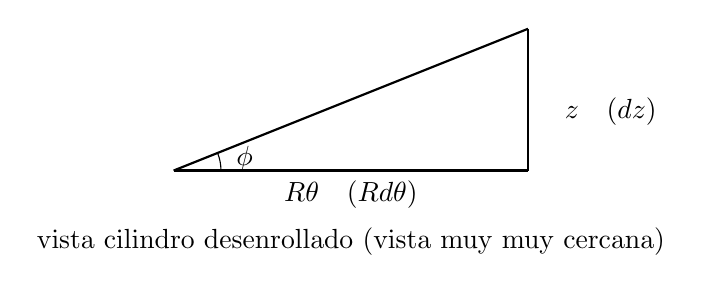
\begin{tikzpicture}[scale=1.5]
    % --- TRIÁNGULO (cilindro desenrollado) ---
    \draw[thick] (0,0) -- (3,1.2); % hipotenusa
    \draw[thick] (0,0) -- (3,0);   % base
    \draw[thick] (3,0) -- (3,1.2); % lado
    % --- ÁNGULO PHI ---
    \draw[dashed] (0,0) -- (0.8,0);
    \draw[dashed] (0,0) -- (0.8,0.32);
    \draw[-] (0.4,0) arc (0:21:0.4);
    \node at (0.6,0.1) {$\phi$};
    % --- ETIQUETAS ---
    \node at (1.5,-0.6) {vista cilindro desenrollado (vista muy muy cercana)};
    \node at (3.7,0.5) {$z\quad(dz)$};
    \node at (1.5,-0.2) {$R\theta \quad(Rd\theta)$};
\end{tikzpicture}
\end{center}
$$\tan(\phi)=\dfrac{z}{R\theta}=\dfrac{dz}{Rd\theta}\longrightarrow z=R\theta\tan(\phi)$$

\patotruco{Como $\phi$ es constante, $z$ queda amarrado a $\theta$ y todo el movimiento depende de una única función $\theta(t)$. Además, en cilíndricas la base se deriva directo: $\dot{\vec{e}}_r=\dot\theta\vec{e}_\theta$ y $\dot{\vec{e}}_\theta=-\dot\theta\vec{e}_r$ (el ``trucazo'', que es el teorema del transporte ya resuelto).}

\textbf{Velocidad}\\
Como se sabe, la velocidad es la derivada temporal de la posición desde un punto fijo.
$$\marc{\vec{v}_P}{N}=\der{\vec{r}_{P}}{N}=\der{(R\vec{e}_r+R)}{N}= R\der{\vec{e}_r}{N}+R\dot\theta\tan(\phi)\vec{e}_z$$
En este caso no es necesario utilizar teorema del transporte porque usamos el trucazo.\\
Derivadas temporales de $\vec{e}_r$ y $\vec{e}_\theta$
$$\transport{\vec{e}_r}{N}{A}=\dot\theta\vec{e}_z\times\vec{e}_r=\dot\theta\vec{e}_\theta $$
$$\transport{\vec{e}_\theta}{N}{A}=\dot\theta\vec{e}_z\times\vec{e}_\theta=-\dot\theta\vec{e}_r $$
y finalmente
$$\marc{\vec{v}_P}{N}=R\dot\theta\vec{e}_\theta+R\dot\theta\tan(\phi)\vec{e}_z$$

\textbf{Aceleración}\\
Al igual que antes podemos simplemente derivar la velocidad para obtener la aceleración.
$$\marc{\vec{a}_P}{N}=\der{\marc{\vec{v}_P}{N}{}}{N}{}=\der{\left(R\dot\theta\vec{e}_\theta+R\dot\theta\tan(\phi)\vec{e}_z\right)}{N}{}=(-R\dot\theta^2)\vec{e}_r+ R\ddot\theta\vec{e}_{\theta}+R\ddot\theta\tan(\phi)\vec{e}_z$$

\textbf{Longitud de arco}\\
La longitud de arco se define como la distancia que recorre la partícula en un lapso de tiempo. Para esto es muy útil saber cuánto recorre en un tiempo ínfimo y se multiplica por el tiempo, así se suma
$$ds=\|\vec{v}_p\|dt\longrightarrow s-s_0=\int\sqrt{R^2\dot\theta^2(1+\tan^2(\phi))}=\int R\dot\theta\sec(\phi)dt$$
Hacemos un cambio de variable, asumiendo que $\theta$ es solo creciente o solo decreciente, es decir, $\dot\theta$ no varía de signo
$$s=\int_{t_0}^t R\dot\theta\sec(\phi)dt\longrightarrow\int_{\theta_0}^\theta R\sec\phi \,\text{d}\theta=R(\theta-\theta_0)\sec(\phi)$$
\respuesta{$\displaystyle s=R\,\theta\sec(\phi)\quad(\theta_0=0)$}
\end{solucion}

\subsubsection{Partícula en mesa circular}
Una partícula, denotada como $P$, se desliza sobre una mesa circular como se muestra en la Figura \ref{fig:masa_circular}. La posición de la partícula se conoce en términos del radio $r$ y el ángulo $\theta$, donde $r$ se mide desde el centro de la mesa en el punto $O$ y $\theta$ se mide en relación con la dirección de $\overline{OQ}$, donde $Q$ es un punto en la circunferencia de la mesa. Sabiendo que la mesa rota con una velocidad angular constante $\Omega$, utilizando el "Teorema de Transporte", determine lo siguiente para un observador en un marco de referencia fijo:

\begin{enumerate}
    \item Los marcos de referencia y sistemas de coordenadas adecuados para describir el movimiento.
    \item El vector posición de la partícula $P$ respecto al centro $O$.
    \item Los vectores de velocidad y aceleración de la partícula $P$ respecto al suelo.
\end{enumerate}

\begin{figure}[!ht]
    \centering
    \begin{tikzpicture}[>=Latex, scale=1.8]
        % --- Parámetros Geométricos ---
        \def\R{1.8}          % Radio de la mesa
        \def\rPos{1.1}        % Distancia radial de P
        \def\angQ{30}         % Orientación de la línea de referencia Q
        \def\thetaAng{40}     % Ángulo theta relativo a OQ

        % --- 1. Mesa Circular ---
        \shadedraw[inner color=white, outer color=gray!40, draw=black, thick] (0,0) circle (\R);
        \filldraw (0,0) circle (1.5pt) node[below left] {$O$};

        % --- 2. Referencia rotatoria en la mesa (OQ) ---
        \coordinate (Q) at (\angQ:\R);
        \draw[thick, dashed] (0,0) -- (Q) node[right] {$Q$};
        
        % --- 3. Posición de la partícula P ---
        % El ángulo absoluto en el dibujo es angQ + thetaAng
        \coordinate (P) at ({\angQ + \thetaAng}:\rPos);
        \draw[->, thick] (0,0) -- (P) node[midway, left] {$r$};
        \filldraw (P) circle (2pt) node[right, xshift=2pt] {$P$};

        % --- 4. Representación del Ángulo Theta ---
        \draw[->] (\angQ:0.7) arc (\angQ:{\angQ+\thetaAng}:0.7);
        \node at ({\angQ + 0.5*\thetaAng}:0.9) {$\theta$};

        % --- 5. Velocidad angular Omega de la mesa ---
        \draw[->, thick] (220:0.4) arc (220:500:0.4);
        \node[below] at (0, -0.45) {$\Omega$};

    \end{tikzpicture}
    \caption{Esquema de una partícula $P$ moviéndose sobre una mesa circular que rota con una velocidad angular constante $\Omega$.}
    \label{fig:masa_circular}
\end{figure}

\ifmostrarSolucion
\begin{tcolorbox}[title=Barra articulada a argolla circular,breakable]
\end{tcolorbox}
\fi

% =========================================================================
% Capítulo 1: Cinemática
% Tema 01: Coordenadas cilíndricas
% Problema 11: Disco en eje giratorio horizontal
% =========================================================================
\subsubsection{Disco en eje giratorio horizontal}

Un disco circular de radio $R$ se une a un eje giratorio de longitud $L$, como se muestra en la Figura \ref{fig:disco_eje_horizontal}. El eje gira respecto de la dirección horizontal con una velocidad angular constante $\Omega$ con respecto al suelo. El disco, a su vez, gira libremente en torno a su centro en el punto $O$. El ángulo $\theta$ describe la posición de un punto $P$ ubicado en el borde del disco relativo al centro del mismo. Utilizando los parámetros indicados, realice lo siguiente:

\begin{enumerate}
    \item Defina los marcos de referencia y los sistemas de coordenadas adecuados para describir el movimiento del sistema desde la perspectiva del suelo.
    \item Determine el vector posición del punto $P$ respecto al punto de apoyo $A$.
    \item Obtenga las expresiones para los vectores de velocidad angular y aceleración angular del eje y del disco.
    \item Calcule los vectores de velocidad y aceleración del punto $P$ respecto al suelo.
\end{enumerate}

\begin{figure}[!ht]
    \centering
    \begin{tikzpicture}[>=Latex, scale=1.8]
        % --- Parámetros Geométricos ---
        \def\L{3.2}          % Longitud del eje
        \def\R{1.1}          % Radio del disco
        \def\thetaAng{45}    % Ángulo theta para el punto P
        \def\BarThickness{0.06} % Grosor de la barra

        % --- Coordenadas ---
        \coordinate (A) at (0,0);
        \coordinate (O) at (\L,0);
        \coordinate (P) at ($ (O) + ({90-\thetaAng}:\R) $);

        % --- 1. Soporte en A ---
        \fill[pattern=north east lines] (-0.3, -0.4) rectangle (0.3, -0.3);
        \draw[thick] (-0.3, -0.3) -- (0.3, -0.3);
        \draw[thin] (A) -- (-0.15, -0.3);
        \draw[thin] (A) -- (0.15, -0.3);
        
        % Articulación A (Gris oscuro)
        \filldraw[fill=gray!80, draw=black] (A) circle (1.8pt) node[below left] {$A$};
    \shadedraw[inner color=white, outer color=gray!40, draw=black, thick] (O) circle (\R);
        % --- 2. Eje Giratorio (Barra L) ---
        \begin{scope}
            \shadedraw[inner color=white, outer color=gray!30, draw=black, rounded corners=2pt] 
                (0, -\BarThickness) rectangle (\L+0.1, \BarThickness);
        \end{scope}
        
        % Velocidad angular Omega
        \draw[->, thick] (1.2, 0.4) arc (60:300:0.2 and 0.4);
        \node[above] at (1.2, 0.4) {$\Omega$};
        
        % Cota de longitud L
        \draw[<->] (0, -0.6) -- (\L, -0.6) node[midway, fill=white] {$L$};
        \draw[dotted] (0, -0.1) -- (0, -0.7);
        \draw[dotted] (\L, -0.1) -- (\L, -0.7);

        % --- 3. Disco en O ---
        
        \draw[dashed] (O) -- ($(O) + (0, \R)$); % Referencia vertical
        
        % Radio R y Ángulo Theta
        \draw[->] (O) -- (P) node[midway, right] {$R$};
        \draw[->] ($(O) + (0, 0.5)$) arc (90:{90-\thetaAng}:0.5);
        \node at ($ (O) + (70:0.75) $) {$\theta$};

        % Articulación O (Gris oscuro)
        \filldraw[fill=gray!80, draw=black] (O) circle (1.2pt) node[above left, xshift=-2pt] {$O$};
        
        % Punto P
        \filldraw (P) circle (1.5pt) node[above right] {$P$};

    \end{tikzpicture}
    \caption{Representación esquemática de un disco de radio $R$ montado en un eje giratorio horizontal de longitud $L$.}
    \label{fig:disco_eje_horizontal}
\end{figure}

% --- SOLUCIÓN ---------------------------------------------------------------
\begin{solucion}{Disco en eje giratorio horizontal}
Lo primero que hacemos es definir los marcos de referencia, con los cuales trabajaremos durante el ejercicio.
\begin{itemize}
    \item $\mathcal{N}$ Suelo (Inercial) $\{\vec{E_x},\vec{E_y},\vec{E_z}\}$
    \item $\mathcal{A}$ Barra $AO$ $\{\vec{e_x},\vec{e_y},\vec{e_z}\}$
    \item $\mathcal{B}$ Disco  $\{\vec{e}_r,\vec{e}_\theta,\vec{e}_z\}$
\end{itemize}

\begin{center}
        \begin{tikzpicture}[>=Latex, scale=1.8]
        % --- Parámetros Geométricos ---
        \def\L{3.2}          % Longitud del eje
        \def\R{1.1}          % Radio del disco
        \def\thetaAng{45}    % Ángulo theta para el punto P
        \def\BarThickness{0.06} % Grosor de la barra

        % --- Coordenadas ---
        \coordinate (A) at (0,0);
        \coordinate (O) at (\L,0);
        \coordinate (P) at ($ (O) + ({90-\thetaAng}:\R) $);

        % --- 1. Soporte en A ---
        \fill[pattern=north east lines] (-0.3, -0.4) rectangle (0.3, -0.3);
        \draw[thick] (-0.3, -0.3) -- (0.3, -0.3);
        \draw[thin] (A) -- (-0.15, -0.3);
        \draw[thin] (A) -- (0.15, -0.3);
        
        % Articulación A (Gris oscuro)
        \filldraw[fill=gray!80, draw=black] (A) circle (1.8pt) node[below left] {$A$};
    \shadedraw[inner color=white, outer color=gray!40, draw=black, thick] (O) circle (\R);
        % --- 2. Eje Giratorio (Barra L) ---
        \begin{scope}
            \shadedraw[inner color=white, outer color=gray!30, draw=black, rounded corners=2pt] 
                (0, -\BarThickness) rectangle (\L+0.1, \BarThickness);
        \end{scope}
        
        % Velocidad angular Omega
        \draw[->, thick] (1.2, 0.4) arc (60:300:0.2 and 0.4);
        \node[above] at (1.2, 0.4) {$\Omega$};
        
        % Cota de longitud L
        \draw[<->] (0, -0.6) -- (\L, -0.6) node[midway, below] {$L$};
        \draw[dotted] (0, -0.1) -- (0, -0.7);
        \draw[dotted] (\L, -0.1) -- (\L, -0.7);

        % --- 3. Disco en O ---
        
        \draw[dashed] (O) -- ($(O) + (0, \R)$); % Referencia vertical
        
        % Radio R y Ángulo Theta
        \draw[->] (O) -- (P) node[midway, right] {$R$};
        \draw[->] ($(O) + (0, 0.5)$) arc (90:{90-\thetaAng}:0.5);
        \node at ($ (O) + (70:0.75) $) {$\theta$};

        % Articulación O (Gris oscuro)
        \filldraw[fill=gray!80, draw=black] (O) circle (1.2pt) node[above left, xshift=-2pt] {$O$};
        
        % Punto P
        \filldraw (P) circle (1.5pt) node[above right] {$P$};

        %aqui van los vectores
        \draw[->, thick, red] (0,0)--++(0.5,0) node[below] {$\vec{E}_y$};
        \draw[->, thick, red] (0,0)--++(0,0.5) node[above] {$\vec{E}_z$};
        
        %aqui van los vectores
        \draw[->, thick, blue] (\L,0)--++(0.7,0) node[below] {$\vec{e}_x$};
        \draw[->, thick, blue] (\L,0)--++(0,0.7) node[above] {$\vec{e}_y$};
        %aqui van los vectores
        \draw[->, thick, green] (\L,0)--++(45:0.7) node[above] {$\vec{e}_r$};
        \draw[->, thick, green] (\L,0)--++(-45:0.7) node[below] {$\vec{e}_\theta$};

    \end{tikzpicture}
\end{center}
\end{solucion}


% =========================================================================
% Capítulo 1: Cinemática
% Tema 01: Coordenadas cilíndricas
% Problema 13: Disco rotante
% =========================================================================
% NOTA: el archivo original estaba vacío; el enunciado se reconstruyó a
% partir de los datos de la solución. Revisar.
\subsubsection{Disco rotante}
Un disco gira con velocidad angular constante $\Omega$ alrededor de su eje, que es fijo al
suelo. Un punto $P$ se mueve radialmente sobre el disco, alejándose del centro con rapidez
constante $v$ relativa al disco, de modo que $r(t) = r_0 + vt$ y $\theta(t) = \Omega t$.
Determine, para un observador fijo al suelo:
\begin{enumerate}
    \item La velocidad del punto $P$.
    \item La aceleración del punto $P$.
    \item Las componentes de la aceleración y su interpretación física.
\end{enumerate}

% --- SOLUCIÓN ---------------------------------------------------------------
\begin{solucion}{Disco rotante}
\subsubsection*{Pregunta 1: Velocidad del punto P}

En coordenadas cilíndricas, la posición del punto es:
$$\vec{r} = r(t) \, \hat{e}_r + z \, \hat{e}_z$$

Con $r(t) = r_0 + vt$ (movimiento radial constante) y $\theta(t) = \Omega t$ (rotación a velocidad angular constante).

La velocidad en coordenadas cilíndricas es:
$$\vec{v} = \dot{r} \, \hat{e}_r + r \dot{\theta} \, \hat{e}_\theta + \dot{z} \, \hat{e}_z$$

Sustituyendo nuestras funciones:
\begin{equation}
\boxed{\vec{v} = v \, \hat{e}_r + (r_0 + vt) \Omega \, \hat{e}_\theta}
\end{equation}

Interpretación:
\begin{itemize}
    \item \textbf{Componente radial}: $v_r = v$ (constante, movimiento hacia afuera)
    \item \textbf{Componente transversal}: $v_\theta = (r_0 + vt) \Omega$ (aumenta con el tiempo)
    \item \textbf{Magnitud de velocidad}: $|\vec{v}| = \sqrt{v^2 + [(r_0 + vt) \Omega]^2}$
\end{itemize}

\subsubsection*{Pregunta 2: Aceleración del punto P}

La aceleración en coordenadas cilíndricas es:
$$\vec{a} = (\ddot{r} - r\dot{\theta}^2) \hat{e}_r + (r\ddot{\theta} + 2\dot{r}\dot{\theta}) \hat{e}_\theta + \ddot{z} \, \hat{e}_z$$

Con nuestras funciones:
\begin{itemize}
    \item $\dot{r} = v$ (velocidad radial constante)
    \item $\ddot{r} = 0$ (aceleración radial nula)
    \item $\dot{\theta} = \Omega$ (velocidad angular constante)
    \item $\ddot{\theta} = 0$ (aceleración angular nula)
    \item $r = r_0 + vt$
\end{itemize}

Sustituyendo:
\begin{equation}
\vec{a} = [0 - (r_0 + vt)\Omega^2] \hat{e}_r + [0 + 2v\Omega] \hat{e}_\theta
\end{equation}

\begin{equation}
\boxed{\vec{a} = -(r_0 + vt) \Omega^2 \, \hat{e}_r + 2v\Omega \, \hat{e}_\theta}
\end{equation}

\subsubsection*{Pregunta 3: Componentes de Aceleración}

\paragraph{Componente Radial (Centrípeta)}
$$a_r = -(r_0 + vt) \Omega^2$$

Esta es la aceleración \textbf{centrípeta}: negativa (apunta hacia el centro), proporcional a la distancia radial, y proporcional al cuadrado de la velocidad angular. Su magnitud aumenta linealmente con el tiempo.

\paragraph{Componente Transversal (Coriolis)}
$$a_\theta = 2v\Omega$$

Esta es la aceleración de \textbf{Coriolis}: es constante, proporcional a la velocidad radial $v$ y a la velocidad angular $\Omega$. Representa el cambio de dirección de la velocidad debido a la rotación del sistema.

\paragraph{Componente Axial}
$$a_z = 0$$

No hay movimiento en la dirección axial (perpendicular al disco).

\paragraph{Magnitud Total}
\begin{equation}
|\vec{a}| = \sqrt{[(r_0 + vt) \Omega^2]^2 + (2v\Omega)^2}
\end{equation}

\paragraph{Interpretación Física}

El término centrípeto $-(r_0 + vt) \Omega^2$ es necesario para mantener el punto en una trayectoria circular alrededor del eje mientras se aleja del centro. El término de Coriolis $2v\Omega$ resulta del hecho de que la velocidad del punto en la dirección transversal $v_\theta = (r_0 + vt) \Omega$ cambia continuamente debido al movimiento radial: conforme el punto se aleja del eje, su velocidad tangencial aumenta, requiriendo una aceleración tangencial.
\end{solucion}

% =========================================================================
% Capítulo 1: Cinemática
% Tema 01: Coordenadas cilíndricas
% Problema 14: Movimiento en Espiral Logarítmica
% =========================================================================
\subsubsection{Movimiento en Espiral Logarítmica}

Un punto $P$ sigue una trayectoria en espiral logarítmica descrita en coordenadas cilíndricas por:
$$r(\theta) = r_0 e^{-k\theta}$$

donde $r_0$ es el radio inicial, $k$ es una constante positiva de amortiguamiento, y $\theta$ es el ángulo azimutal. El punto se desplaza de modo que su velocidad angular es constante: $\dot{\theta} = \omega_0$.

\begin{enumerate}
    \item Expresar la velocidad del punto en coordenadas cilíndricas.
    \item Calcular la aceleración del punto.
    \item Demostrar que la rapidez (magnitud de velocidad) decrece exponencialmente con el tiempo.
\end{enumerate}

\begin{figure}[!ht]
    \centering
    \begin{tikzpicture}[>=Latex, scale=1.6]

        % --- CONFIGURACIÓN DE PARÁMETROS ---
        \def\ro{2.5}      % Radio inicial r0 [cm]
        \def\k{0.15}      % Constante de amortiguamiento k
        \def\w{1}         % Escala de la espiral

        % --- SOPORTES Y ELEMENTOS FIJOS ---
        % Origen
        \coordinate (O) at (0,0);
        \filldraw (O) circle (1.5pt) node[above left] {$O$};

        % --- GEOMETRÍA PRINCIPAL ---
        % Espiral logarítmica (dibujada como varios puntos conectados)
        \draw[thick, azul]
            plot[parametric, samples=100, domain=0:3*pi]
            ({0.8*\ro*exp(-\k*\x/pi)*cos(\x r)}, {0.8*\ro*exp(-\k*\x/pi)*sin(\x r)});

        % --- SISTEMAS DE COORDENADAS ---
        % Ejes de referencia
        \draw[->, thick] (O) -- (3, 0) node[right, font=\small] {$x$};
        \draw[->, thick] (O) -- (0, 3) node[above, font=\small] {$y$};

        % --- PUNTOS Y COORDENADAS ---
        % Punto inicial en la espiral (t=0)
        \coordinate (P0) at (0.8*\ro, 0);
        \filldraw[fill=white, thick] (P0) circle (2.5pt);
        \filldraw (P0) circle (1pt) node[right, font=\small] {$P(t=0)$};

        % Punto en tiempo intermedio
        \coordinate (Pm) at ({0.8*\ro*exp(-\k*pi/2)*cos(pi/2 r)}, {0.8*\ro*exp(-\k*pi/2)*sin(pi/2 r)});
        \filldraw[fill=white, thick] (Pm) circle (2pt);
        \filldraw (Pm) circle (1pt);

        % Punto cerca del origen (t grande)
        \coordinate (Pf) at ({0.8*\ro*exp(-\k*3*pi)*cos(3*pi r)}, {0.8*\ro*exp(-\k*3*pi)*sin(3*pi r)});
        \filldraw[fill=white, thick] (Pf) circle (2pt);
        \filldraw (Pf) circle (1pt) node[left, font=\small] {$P(t \to \infty)$};

        % --- VECTORES Y FUERZAS ---
        % Vector de velocidad en el punto inicial
        % Velocidad radial (hacia adentro) + velocidad tangencial
        \draw[->, thick, myred] (P0) -- ($(P0) + (-0.4, 0)$) node[below, font=\small, color=myred] {$\vec{v}_r$};
        \draw[->, thick, orange] (P0) -- ($(P0) + (0, 0.5)$) node[above, font=\small, color=orange] {$\vec{v}_\theta$};

        % Vector velocidad total (resultante)
        \draw[->, thick, gris1] (P0) -- ($(P0) + (-0.4, 0.5)$) node[above right, font=\small, color=gris1] {$\vec{v}$};

        % --- ANOTACIONES Y ETIQUETAS ---
        % Ángulo theta en un punto
        \draw[dashed, gray] (0, 0) -- (Pm);
        \draw[->, dashed, gray] (0.5, 0) arc (0:90:0.5);
        \node at (0.6, 0.4) [font=\small] {$\theta$};

        % Radio en el punto inicial
        \draw[<->, thin, gray] (0, -0.35) -- (P0) node[midway, below, font=\small] {$r_0$};

        % Etiqueta
        \node[font=\footnotesize] at (1.5, -2) {Espiral logarítmica: $r(\theta) = r_0 e^{-k\theta}$};

    \end{tikzpicture}
    \caption{Trayectoria en espiral logarítmica con velocidad descompuesta en componentes radial y transversal}
    \label{fig:c1_e01_p05_espiral}
\end{figure}

% --- SOLUCIÓN ---------------------------------------------------------------
\begin{solucion}{Espiral logarítmica}
\subsubsection*{Pregunta 1: Velocidad en Coordenadas Cilíndricas}

Dado que $\theta(t) = \omega_0 t$ (velocidad angular constante), tenemos $\dot{\theta} = \omega_0$ y $\ddot{\theta} = 0$.

De la ecuación de la espiral $r(\theta) = r_0 e^{-k\theta}$, obtenemos $r(t) = r_0 e^{-k\omega_0 t}$.

Derivando respecto al tiempo:
$$\dot{r} = r_0 \cdot (-k\omega_0) e^{-k\omega_0 t} = -k\omega_0 \cdot r_0 e^{-k\omega_0 t} = -k\omega_0 \cdot r(t)$$

La velocidad en coordenadas cilíndricas es:
$$\vec{v} = \dot{r} \, \hat{e}_r + r\dot{\theta} \, \hat{e}_\theta$$

Sustituyendo:
\begin{equation}
\boxed{\vec{v} = -k\omega_0 r(t) \, \hat{e}_r + r(t) \omega_0 \, \hat{e}_\theta = \omega_0 r(t) \left[ -k \, \hat{e}_r + \hat{e}_\theta \right]}
\end{equation}

\subsubsection*{Pregunta 2: Aceleración del Punto}

La aceleración en coordenadas cilíndricas es:
$$\vec{a} = (\ddot{r} - r\dot{\theta}^2) \hat{e}_r + (r\ddot{\theta} + 2\dot{r}\dot{\theta}) \hat{e}_\theta$$

Calculamos las derivadas necesarias:
\begin{itemize}
    \item $\dot{r} = -k\omega_0 r(t)$
    \item $\ddot{r} = -k\omega_0 \dot{r} = -k\omega_0 \cdot (-k\omega_0 r) = k^2 \omega_0^2 r(t)$
    \item $\dot{\theta} = \omega_0$
    \item $\ddot{\theta} = 0$
\end{itemize}

Componente radial:
$$a_r = \ddot{r} - r\dot{\theta}^2 = k^2 \omega_0^2 r - r \omega_0^2 = (k^2 - 1) \omega_0^2 r$$

Componente transversal:
$$a_\theta = r \cdot 0 + 2 \cdot (-k\omega_0 r) \cdot \omega_0 = -2k\omega_0^2 r$$

La aceleración total es:
\begin{equation}
\boxed{\vec{a} = (k^2 - 1) \omega_0^2 r(t) \, \hat{e}_r - 2k\omega_0^2 r(t) \, \hat{e}_\theta}
\end{equation}

o, factorizando:
\begin{equation}
\vec{a} = \omega_0^2 r(t) \left[ (k^2 - 1) \hat{e}_r - 2k \, \hat{e}_\theta \right]
\end{equation}

\paragraph{Análisis de la Aceleración}

\begin{itemize}
    \item Si $k < 1$: La componente radial apunta hacia afuera (positiva), aunque el punto se acerca al origen. Esto ocurre porque la velocidad radial disminuye en magnitud; el cambio de velocidad radial implica aceleración hacia afuera.
    \item Si $k = 1$: La componente radial es cero; solo existe aceleración transversal (similar a movimiento circular uniforme de radio variable).
    \item Si $k > 1$: La componente radial apunta hacia adentro, acelerando la convergencia.
    \item La componente transversal $a_\theta = -2k\omega_0^2 r$ siempre apunta en dirección negativa (contraria a la velocidad angular), ralentizando la rotación.
\end{itemize}

\subsubsection*{Pregunta 3: Rapidez Exponencial Decreciente}

La rapidez (magnitud de velocidad) es:
$$v = |\vec{v}| = \sqrt{(\dot{r})^2 + (r\dot{\theta})^2} = \sqrt{k^2\omega_0^2 r^2 + r^2 \omega_0^2}$$

$$v = \omega_0 r \sqrt{k^2 + 1} = \omega_0 \sqrt{k^2 + 1} \cdot r_0 e^{-k\omega_0 t}$$

\begin{equation}
\boxed{v(t) = v_0 e^{-k\omega_0 t}}
\end{equation}

donde $v_0 = \omega_0 r_0 \sqrt{k^2 + 1}$ es la rapidez inicial.

\paragraph{Demostración}

La rapidez disminuye exponencialmente con constante de tiempo $\tau = 1/(k\omega_0)$. Conforme $t \to \infty$:
- $r(t) \to 0$ (el punto converge al origen)
- $v(t) \to 0$ (la velocidad tiende a cero)
- El punto completa infinitas revoluciones alrededor del origen en tiempo finito, pero su velocidad disminuye exponencialmente.

Este comportamiento es típico de sistemas disipativos donde la energía cinética se reduce continuamente.
\end{solucion}


\newpage
\subsection{Soluciones del Tema 01}

% =========================================================================
% Solución: C1_E01_P04 - Disco Rotante con Punto en Movimiento Radial
% =========================================================================

\begin{sol}[Tema: Cinemática en Coordenadas Cilíndricas - Disco Rotante]

\subsubsection*{Pregunta 1: Velocidad del punto P}

En coordenadas cilíndricas, la posición del punto es:
$$\vec{r} = r(t) \, \hat{e}_r + z \, \hat{e}_z$$

Con $r(t) = r_0 + vt$ (movimiento radial constante) y $\theta(t) = \Omega t$ (rotación a velocidad angular constante).

La velocidad en coordenadas cilíndricas es:
$$\vec{v} = \dot{r} \, \hat{e}_r + r \dot{\theta} \, \hat{e}_\theta + \dot{z} \, \hat{e}_z$$

Sustituyendo nuestras funciones:
\begin{equation}
\boxed{\vec{v} = v \, \hat{e}_r + (r_0 + vt) \Omega \, \hat{e}_\theta}
\end{equation}

Interpretación:
\begin{itemize}
    \item \textbf{Componente radial}: $v_r = v$ (constante, movimiento hacia afuera)
    \item \textbf{Componente transversal}: $v_\theta = (r_0 + vt) \Omega$ (aumenta con el tiempo)
    \item \textbf{Magnitud de velocidad}: $|\vec{v}| = \sqrt{v^2 + [(r_0 + vt) \Omega]^2}$
\end{itemize}

\subsubsection*{Pregunta 2: Aceleración del punto P}

La aceleración en coordenadas cilíndricas es:
$$\vec{a} = (\ddot{r} - r\dot{\theta}^2) \hat{e}_r + (r\ddot{\theta} + 2\dot{r}\dot{\theta}) \hat{e}_\theta + \ddot{z} \, \hat{e}_z$$

Con nuestras funciones:
\begin{itemize}
    \item $\dot{r} = v$ (velocidad radial constante)
    \item $\ddot{r} = 0$ (aceleración radial nula)
    \item $\dot{\theta} = \Omega$ (velocidad angular constante)
    \item $\ddot{\theta} = 0$ (aceleración angular nula)
    \item $r = r_0 + vt$
\end{itemize}

Sustituyendo:
\begin{equation}
\vec{a} = [0 - (r_0 + vt)\Omega^2] \hat{e}_r + [0 + 2v\Omega] \hat{e}_\theta
\end{equation}

\begin{equation}
\boxed{\vec{a} = -(r_0 + vt) \Omega^2 \, \hat{e}_r + 2v\Omega \, \hat{e}_\theta}
\end{equation}

\subsubsection*{Pregunta 3: Componentes de Aceleración}

\paragraph{Componente Radial (Centrípeta)}
$$a_r = -(r_0 + vt) \Omega^2$$

Esta es la aceleración \textbf{centrípeta}: negativa (apunta hacia el centro), proporcional a la distancia radial, y proporcional al cuadrado de la velocidad angular. Su magnitud aumenta linealmente con el tiempo.

\paragraph{Componente Transversal (Coriolis)}
$$a_\theta = 2v\Omega$$

Esta es la aceleración de \textbf{Coriolis}: es constante, proporcional a la velocidad radial $v$ y a la velocidad angular $\Omega$. Representa el cambio de dirección de la velocidad debido a la rotación del sistema.

\paragraph{Componente Axial}
$$a_z = 0$$

No hay movimiento en la dirección axial (perpendicular al disco).

\paragraph{Magnitud Total}
\begin{equation}
|\vec{a}| = \sqrt{[(r_0 + vt) \Omega^2]^2 + (2v\Omega)^2}
\end{equation}

\paragraph{Interpretación Física}

El término centrípeto $-(r_0 + vt) \Omega^2$ es necesario para mantener el punto en una trayectoria circular alrededor del eje mientras se aleja del centro. El término de Coriolis $2v\Omega$ resulta del hecho de que la velocidad del punto en la dirección transversal $v_\theta = (r_0 + vt) \Omega$ cambia continuamente debido al movimiento radial: conforme el punto se aleja del eje, su velocidad tangencial aumenta, requiriendo una aceleración tangencial.

\end{sol}


\newpage
% =========================================================================
% Solución: C1_E01_P05 - Movimiento en Espiral Logarítmica
% =========================================================================

\begin{sol}[Tema: Cinemática en Coordenadas Cilíndricas - Espiral Logarítmica]

\subsubsection*{Pregunta 1: Velocidad en Coordenadas Cilíndricas}

Dado que $\theta(t) = \omega_0 t$ (velocidad angular constante), tenemos $\dot{\theta} = \omega_0$ y $\ddot{\theta} = 0$.

De la ecuación de la espiral $r(\theta) = r_0 e^{-k\theta}$, obtenemos $r(t) = r_0 e^{-k\omega_0 t}$.

Derivando respecto al tiempo:
$$\dot{r} = r_0 \cdot (-k\omega_0) e^{-k\omega_0 t} = -k\omega_0 \cdot r_0 e^{-k\omega_0 t} = -k\omega_0 \cdot r(t)$$

La velocidad en coordenadas cilíndricas es:
$$\vec{v} = \dot{r} \, \hat{e}_r + r\dot{\theta} \, \hat{e}_\theta$$

Sustituyendo:
\begin{equation}
\boxed{\vec{v} = -k\omega_0 r(t) \, \hat{e}_r + r(t) \omega_0 \, \hat{e}_\theta = \omega_0 r(t) \left[ -k \, \hat{e}_r + \hat{e}_\theta \right]}
\end{equation}

\subsubsection*{Pregunta 2: Aceleración del Punto}

La aceleración en coordenadas cilíndricas es:
$$\vec{a} = (\ddot{r} - r\dot{\theta}^2) \hat{e}_r + (r\ddot{\theta} + 2\dot{r}\dot{\theta}) \hat{e}_\theta$$

Calculamos las derivadas necesarias:
\begin{itemize}
    \item $\dot{r} = -k\omega_0 r(t)$
    \item $\ddot{r} = -k\omega_0 \dot{r} = -k\omega_0 \cdot (-k\omega_0 r) = k^2 \omega_0^2 r(t)$
    \item $\dot{\theta} = \omega_0$
    \item $\ddot{\theta} = 0$
\end{itemize}

Componente radial:
$$a_r = \ddot{r} - r\dot{\theta}^2 = k^2 \omega_0^2 r - r \omega_0^2 = (k^2 - 1) \omega_0^2 r$$

Componente transversal:
$$a_\theta = r \cdot 0 + 2 \cdot (-k\omega_0 r) \cdot \omega_0 = -2k\omega_0^2 r$$

La aceleración total es:
\begin{equation}
\boxed{\vec{a} = (k^2 - 1) \omega_0^2 r(t) \, \hat{e}_r - 2k\omega_0^2 r(t) \, \hat{e}_\theta}
\end{equation}

o, factorizando:
\begin{equation}
\vec{a} = \omega_0^2 r(t) \left[ (k^2 - 1) \hat{e}_r - 2k \, \hat{e}_\theta \right]
\end{equation}

\paragraph{Análisis de la Aceleración}

\begin{itemize}
    \item Si $k < 1$: La componente radial apunta hacia afuera (positiva), aunque el punto se acerca al origen. Esto ocurre porque la velocidad radial disminuye en magnitud; el cambio de velocidad radial implica aceleración hacia afuera.
    \item Si $k = 1$: La componente radial es cero; solo existe aceleración transversal (similar a movimiento circular uniforme de radio variable).
    \item Si $k > 1$: La componente radial apunta hacia adentro, acelerando la convergencia.
    \item La componente transversal $a_\theta = -2k\omega_0^2 r$ siempre apunta en dirección negativa (contraria a la velocidad angular), ralentizando la rotación.
\end{itemize}

\subsubsection*{Pregunta 3: Rapidez Exponencial Decreciente}

La rapidez (magnitud de velocidad) es:
$$v = |\vec{v}| = \sqrt{(\dot{r})^2 + (r\dot{\theta})^2} = \sqrt{k^2\omega_0^2 r^2 + r^2 \omega_0^2}$$

$$v = \omega_0 r \sqrt{k^2 + 1} = \omega_0 \sqrt{k^2 + 1} \cdot r_0 e^{-k\omega_0 t}$$

\begin{equation}
\boxed{v(t) = v_0 e^{-k\omega_0 t}}
\end{equation}

donde $v_0 = \omega_0 r_0 \sqrt{k^2 + 1}$ es la rapidez inicial.

\paragraph{Demostración}

La rapidez disminuye exponencialmente con constante de tiempo $\tau = 1/(k\omega_0)$. Conforme $t \to \infty$:
- $r(t) \to 0$ (el punto converge al origen)
- $v(t) \to 0$ (la velocidad tiende a cero)
- El punto completa infinitas revoluciones alrededor del origen en tiempo finito, pero su velocidad disminuye exponencialmente.

Este comportamiento es típico de sistemas disipativos donde la energía cinética se reduce continuamente.

\end{sol}


\newpage
% =========================================================================
% Capítulo 1 - Tema 02: Cinemática en Coordenadas Esféricas
% =========================================================================

\section{Tema 02: Cinemática en Coordenadas Esféricas}

Las coordenadas esféricas son naturales para problemas con simetría central,
como el movimiento de péndulos esféricos o trayectorias sobre superficies curvas.

\subsection{Ejercicios}

\subsubsection{Problema: Anillo rotador}
Un anillo \( P \) se desliza a lo largo de un aro circular de radio \( r \) como indica la figura \ref{fig:anillo_deslizante}. El aro rota con una velocidad angular \( \Omega \) que apunta en la dirección vertical gracias a las uniones en \( A \) y \( B \), que en conjunto actúan como una conexión de revolución.

Si el ángulo \( \phi \) describe la posición del anillo con respecto al centro \( O \) del aro circular, determine:

\begin{enumerate}
    
    \item Marcos de referencia y Sistemas de coordenadas.
    \item La posición del anillo \( P \).
    \item La velocidad y aceleración angular del anillo \( P \).
    \item La velocidad y aceleración del anillo \( P \) vistos por un observador fijo en \( O \).
\end{enumerate}

\begin{figure}[!ht]
    \centering
    \begin{tikzpicture}[>=Latex, scale=1]
        % --- Parámetros Geométricos ---
        \pgfmathsetmacro{\Rout}{2.2} % Radio exterior del anillo
        \pgfmathsetmacro{\Rin}{2.0}  % Radio interior del anillo
        \pgfmathsetmacro{\Rmid}{(\Rin+\Rout)/2} % Radio medio (para P)
        \def\ThetaAngle{50}             % Ángulo theta desde la vertical

        \coordinate (O) at (0,0);

        % --- 1. Eje Central y Centro ---
        \draw[dash dot, thin] (0, -\Rout - 1.5) -- (0, \Rout + 1.8);
        \filldraw (O) circle (1.5pt) node[left, xshift=-2pt] {$O$};

        % --- 2. Anillo Circular ---
        % Relleno gris entre dos círculos para dar grosor (even odd rule)
        \draw[fill=gray!35, thick, even odd rule] (O) circle (\Rout) (O) circle (\Rin);

        % --- 3. Soporte Superior A ---
        \begin{scope}[shift={(0, \Rout)}]
            % Pieza en T (móvil, unida al anillo)
            \draw[fill=gray!50, thick] (-0.15, 0) rectangle (0.15, 0.3);
            \draw[fill=gray!50, thick] (-0.4, 0.3) rectangle (0.4, 0.6);
            % Guía Fija (C negra)
            \draw[fill=black] (-0.6, 0.2) rectangle (0.6, 0.7);
            \draw[fill=white, thick] (-0.42, 0.18) rectangle (0.42, 0.62);
            % Techo fijo (rayado)
            \draw[thick, pattern=north east lines] (-0.7, 0.7) rectangle (0.7, 1.0);
            \draw[thick] (-0.7, 0.7) -- (0.7, 0.7);
            \node[left] at (-0.6, 0.35) {$A$};
        \end{scope}

        % --- 4. Soporte Inferior B (Espejo de A) ---
        \begin{scope}[shift={(0, -\Rout)}, rotate=180]
            \draw[fill=gray!50, thick] (-0.15, 0) rectangle (0.15, 0.3);
            \draw[fill=gray!50, thick] (-0.4, 0.3) rectangle (0.4, 0.6);
            \draw[fill=black] (-0.6, 0.2) rectangle (0.6, 0.7);
            \draw[fill=white, thick] (-0.42, 0.18) rectangle (0.42, 0.62);
            \draw[thick, pattern=north east lines] (-0.7, 0.7) rectangle (0.7, 1.0);
            \draw[thick] (-0.7, 0.7) -- (0.7, 0.7);
            \node[left] at (0.6, 0.35) {$B$};
        \end{scope}

        % --- 5. Partícula P ---
        % Posición calculada para estar en el medio del grosor del anillo
        \coordinate (P) at ({90-\ThetaAngle}:\Rmid);
        \begin{scope}[shift={(P)}, rotate={90-\ThetaAngle}]
            \draw[fill=gray!40, thick, rounded corners=2pt] (-0.2, -0.12) rectangle (0.2, 0.12);
            \node[above right, xshift=2pt] {$P$};
        \end{scope}

        % --- 6. Vectores y Ángulos ---
        % Vector Posición r
        \draw[->, thick] (O) -- (P) node[midway, right] {$r$};
        % Ángulo Theta desde la vertical
        \draw[->, thick] (0, 1.0) arc (90:{90-\ThetaAngle}:1.0);
        \node at ({90-\ThetaAngle/2}:1.3) {$\theta$};

        % Vector Rotación Omega (Superior)
        \coordinate (TopAxis) at (0, \Rout + 1.3);
        \draw[->, very thick] (TopAxis) -- ++(0, 0.8); 
        \draw[->, thick] ($(TopAxis)+(-0.3,0.3)$) arc (170:370:0.4 and 0.15);
        \node[left] at ($(TopAxis)+(-0.5, 0.4)$) {$\Omega$};

    \end{tikzpicture}
    \caption{Sistema mecánico compuesto por un anillo circular giratorio con soportes deslizantes en $A$ y $B$. La partícula $P$ se desplaza a lo largo del anillo con una posición definida por $r$ y $\theta$.}
    \label{fig:anillo_deslizante}
\end{figure}

\ifmostrarSolucion
\begin{tcolorbox}[title=Anillo rotador,breakable]
\textbf{Marcos de referencia y Sistemas de coordenadas}\\

Lo primero de todo es podes obtener los marcos de referencia y se parte primero con el marco de referencia inercia;\\
En este caso se puede apreciar como parece un sistemas de coordenadas esférico, pero para analizar este sistemas de coordenadas lo que haremos sera un sistema doble cilíndrico, el primero asociado al aro, el el segundo en el aro asociado al anillo, en realidad es así como se define un sistema de coordenadas esférico, a base de dos cilíndricos, uno sobre el otro.
\begin{itemize}
    \item $\mathcal{N}$ El suelo $\longrightarrow\{\vec{E}_x;\vec{E}_y;\vec{E}_z\}$
    \item $\mathcal{A}$ El aro $\longrightarrow\{\vec{e}_x;\vec{e}_y;\vec{e}_z\}$
    \item $\mathcal{B}$ El anillo $\longrightarrow\{\vec{e}_r;\vec{e}_\theta;\vec{e}_\phi\}$
\end{itemize}

En este caso se pueden apreciar 2 sistemas de coordenadas el del marco inercial, y el del marco de referencia $\mathcal{A}$, donde los puntos grises son el anillo cortado. Aparte notar que en la figura \ref{fig:D1} $\Omega$ no es el angulo por si mismo si no que es la velocidad angular de un marco respecto otro


\begin{center}
    % --- INICIO FIGURA 2 ---
    \begin{minipage}{0.48\textwidth}
        \centering
        \begin{tikzpicture}[>=Stealth, scale=1.3]
            % Definición de radio y ángulos
            \def\R{1.6}
            \def\angOmega{55}
            
            % Ejes principales negros
            \draw[<->, thick] (-1.8,0) -- (2.0,0);
            \draw[<->, thick] (0,-1.8) -- (0,2.0);
            
            % Círculo
            \draw (0,0) circle (\R);
            
            % Masas (Puntos grises en el anillo)
            \fill[gray] (\angOmega:\R) circle (3pt);
            \fill[gray] (\angOmega+180:\R) circle (3pt);
            
            % Sistema fijo (Azul)
            \draw[->, blue!70!black, thick] (0,0) -- (1.2,0) node[below right] {$\vec{E}_x$};
            \draw[->, blue!70!black, thick] (0,0) -- (0,1.2) node[above left] {$\vec{E}_y$};
            
            % Sistema móvil (Verde)
            \draw[->, green!40!black, thick] (0,0) -- (\angOmega:1.2) node[above left= -2pt] {$\vec{e}_x$};
            \draw[->, green!40!black, thick] (0,0) -- ({\angOmega+90}:1.2) node[left=2pt] {$\vec{e}_y$};
            
            % Punto P
            \fill (\angOmega:1.2) circle (1.5pt) node[right=2pt] {P};
            
            % Ángulo Omega
            \draw[->] (0.7,0) arc (0:\angOmega:0.7) node[midway, right=1pt] {$\Omega$};
            
            % Origen (Punto saliendo)
            \fill[white] (0,0) circle (4pt);
            \draw (0,0) circle (4pt);
            \fill (0,0) circle (1.5pt);
            \node[below left=2pt] at (0,0) {$\vec{E}_z = \vec{e}_z$};
            
            % Falso Caption
            \vspace{0.5cm}
            \node[below, align=center, text width=6cm] at (0,-2) 
                {\footnotesize \textbf{Figura 2:} Diagrama de corte del anillo};
        \end{tikzpicture}
    \end{minipage}\hfill
    % --- INICIO FIGURA 3 ---
    \begin{minipage}{0.48\textwidth}
        \centering
        \begin{tikzpicture}[>=Stealth, scale=1.3]
            % Definición de radio y ángulos
            \def\R{1.6}
            \def\angTheta{30} % Ángulo desde la horizontal (equivale a theta desde el eje z)
            
            % Ejes principales negros
            \draw[<->, thick] (-1.8,0) -- (2.0,0);
            \draw[<->, thick] (0,-1.8) -- (0,2.0);
            
            % Círculo
            \draw (0,0) circle (\R);
            
            % Sistema marco A (Verde)
            \draw[->, green!40!black, thick] (0,0) -- (1.2,0) node[below right] {$\vec{e}_x$};
            \draw[->, green!40!black, thick] (0,0) -- (0,1.2) node[above left] {$\vec{e}_z$};
            
            % Sistema marco B (Café/Rojo)
            \draw[->, red!40!black, thick] (0,0) -- (\angTheta:1.2) node[above left= -2pt] {$\vec{e}_r$};
            \draw[->, red!40!black, thick] (0,0) -- ({\angTheta-90}:1.2) node[below left] {$\vec{e}_\theta$};
            
            % Punto P en el anillo
            \fill (\angTheta:\R) circle (1.5pt) node[right=2pt] {P};
            
            % Ángulo Theta (Desde e_z hasta e_r)
            \draw[<->] (0,0.8) arc (90:\angTheta:0.8) node[midway, above right=1pt] {$\theta$};
            
            % Origen (Cruz entrando)
            \fill[white] (0,0) circle (4pt);
            \draw (0,0) circle (4pt);
            \draw (-2.5pt,-2.5pt) -- (2.5pt,2.5pt);
            \draw (-2.5pt,2.5pt) -- (2.5pt,-2.5pt);
            \node[below left=2pt] at (0,0) {$\vec{e}_y = \vec{e}_\phi$};
            
            % Falso Caption
            \vspace{0.5cm}
            \node[below, align=center, text width=6cm] at (0,-2) 
                {\footnotesize \textbf{Figura 1} Sist. Coord. marcos $\mathcal{A}, \mathcal{B}$};
        \end{tikzpicture}
    \end{minipage}
\end{center}

\textbf{La posición del anillo \( P \).}\\
Para obtener la posición siempre la tomamos desde un punto inercial (basicamente un punto que no se mueva) por ejemplo el centro  $O$, como también lo podría ser el punto $A$ en este caso demostraremos que da lo mismo el punto que elijamos mientras sea inercial.
$$\vec{r}_{P/A}=\underbrace{\vec{r}_{P/O}}_{r\vec{e}_r} +\underbrace{\vec{r}_{O/A}}_{-r\vec{e}_z}$$

\textbf{La velocidad y aceleración angular del anillo \( P \).}\\
Para este caso se tiene que analizar la velocidad angular se tiene que ver respecto a que ejes son los que giran los marcos de referencia, rapidamente podemos darnos cuenta que $\mathcal{A}$ gira con velocidad $\Omega$ gira con respecto al $\vec{e}_z$ o $\vec{E}_z$ que son el mismo vector, y junto a \ref{fig:D2} se puede ver que el marco de referencia $\mathcal{B}$ gira respecto al $\mathcal{A}$ con velocidad angular $\dot\theta$ en $\vec{e}_{\phi}$, siempre recordar de usar la regla de la mano derecha para saber si es que es positivo o negativo el vector.
$$\velang{N}{A}=\Omega\vec{e}_z$$
$$\velang{A}{B}=\dot\theta\vec{e}_y$$
Pero lo que queremos obtener es la velocidad angular del marco referencia del anillo y lo que tenemos es la del anillo respecto al aro ($\velang{A}B$) y la del aro respecto al suelo $\velang{N}{A}$, pero la velocidad angular cumple la propiedad aditiva, (no se cumple para la aceleración angular.)
$$\velang{N}{B}=\velang{N}{A}+\velang{A}{B}=\dot\theta\vec{e}_y+\Omega\vec{e}_z$$
Ahora solo falta la aceleración angular que se define como 
$$\accang{N}{F} =\der{}{N}\left(\velang{N}{F}\right)$$ ($\mathcal{F}$ es un ejemplo simplemente)\\

Entonces podemos calcularlo

$$\accang{N}{B} =\der{}{N}\left(\velang{N}{B}\right)$$
En este caso decidimos calcularlo respecto al marco $\mathcal{A}$ porque ambos vectores están en fijos a ese marco

$$\accang{N}{B}=\transporta{\velang{N}{B}}{N}{A}$$
$$\accang{N}{B}=\transporta{\left(\dot\theta\vec{e}_y+\Omega\vec{e}_z\right)}{N}{A}$$
$$\accang{N}{B}=\dot\theta\vec{e}_y+\dot\Omega\vec{e}_z-\Omega\dot\theta\vec{e}_x$$
\textbf{La velocidad y aceleración del anillo \( P \) vistos por un observador fijo en \( O \).}
Si bien en este caso dice que sea desde el punto $O$ (deberiamos hacerlo desde $O$) el; hacerlo de cualquier punto (Observador) fijo  también sirve.

$$\marc{\vec{v}_P}{N}=\der{\vec{r}_{P/A}}{N}=\der{(r\vec{e}_r-r\vec{e}_z)}{N}$$
Por propiedades de la derivada podemos separar por la suma y obtenemos
$$\der{\vec{r}_{P/A}}{N}=\der{\vec{r}_{P/O}}{N}+\der{\vec{r}_{O/A}}{N}$$
$$\der{\vec{r}_{O/A}}{N}=\der{(-r\vec{e}_z)}{N}=\transporta{(-r\vec{e}_z)}{N}{A}$$
$$\der{(-r\vec{e}_z)}{A}=\vec{0} \quad\quad \velang{N}{A}\times(-r\vec{e}_z)=\vec{0}$$
Ahora falta $\vec{r}_{P/O}$ (que en este caso usaremos el teorema del transporte respecto a $\mathcal{B}$ ya que tenemos el vector posición en base de $\mathcal{B}$)
$$\der{\vec{r}_{P/O}}{N}=\transporta{(r\vec{e}_r)}{N}{B}$$
$$\der{(r\vec{e}_r)}{B}=\vec{0} \quad\quad \velang{N}{B}\times(r\vec{e}_r)=\left(\dot\theta\vec{e}_y+\Omega\vec{e}_z\right)\times(r\vec{e}_r)$$
Aquí tenemos un problema, no todos los vectores están en la misma base, no sabemos cuanto es $\vec{e}_z\times \vec{e}_r$ paras esto transformaremos el vector $\vec{e}_z$ en la base asociada al marco $\mathcal{B}$

$$\vec{e}_z=\cos{(\theta)}\vec{e}_r-\sin(\theta)\vec{e}_\theta$$
$$\vec{e}_x=\sin{(\theta)}\vec{e}_r+\cos(\theta)\vec{e}_\theta$$
$$\vec{e}_y=\vec{e}_\phi$$
Recuerden siempre que trabajamos tenemos que descomponer el vector completo, no sirve que solo nos quedemos con una componente, para confirmar que es el vector completo se puede sacar la norma y debería dar siempre 1.\\

Ahora que ya tenemos la transformación de $\vec{e}_z$ podemos terminar de calcular la velocidad
$$\der{(r\vec{e}_r)}{B}=\vec{0} $$
$$\velang{N}{B}\times(r\vec{e}_r)=\left(\dot\theta\vec{e}_\phi+\Omega(\cos{(\theta)}\vec{e}_r-\sin(\theta)\vec{e}_\theta))\right)\times(r\vec{e}_r)=r\dot\theta\vec{e}_\theta +r\Omega\sin{(\theta)}\vec{e}_\phi$$

\textbf{Aceleración}\\
Ahora simplemente toca hacer los mismos pasos para la aceleración
$$\der{\marc{}{N}\vec{v}_P}{N}=\transporta{\left(r\dot\theta\vec{e}_\theta +r\Omega\sin{(\theta)}\vec{e}_\phi\right)}{N}{B}$$
$$\der{\left(r\dot\theta\vec{e}_\theta +r\Omega\sin{(\theta)}\vec{e}_\phi\right)}{B}=r\ddot{\theta}\vec{e}_\theta+r\dot\Omega\sin{(\theta)}\vec{e}_\phi+r\Omega\dot\theta\cos{(\theta)}\vec{e}_{\phi}$$

$$\velang{N}{B}\times\left(\marc{\vec{v}}{N}\right)=\left(\dot\theta\vec{e}_\phi+\Omega(\cos{(\theta)}\vec{e}_r-\sin(\theta)\vec{e}_\theta))\right)\times\left(r\dot\theta\vec{e}_\theta +r\Omega\sin{(\theta)}\vec{e}_\phi\right)=$$
$$=r\dot\theta^2 \vec{e}_r+\vec{0}+r\dot\theta\Omega\cos(\theta)\vec{e}_\phi+r\Omega^2\cos(\theta)\sin(\theta)(-\vec{e}_\theta)+r\dot\theta\Omega(-\sin(\theta))\vec{e}_{\phi}-r\Omega^2\sin^2(\theta)(\vec{e}_r)$$

$$\marc{\vec{a}}{N}=\left(-r\dot\theta^2-r\Omega^2\sin^2(\theta)\right)\vec{e}_r+\left(r\ddot{\theta}-r\Omega\sin(\theta)\cos(\theta)\right)\vec{e}_\theta+\left(r\dot\Omega\sin(\theta)+2r\Omega\dot\theta\cos(\theta)\right)\vec{e}_\phi$$

\end{tcolorbox}
\fi

\subsubsection{Curva espiral en coordenadas esféricas}

Considere una curva espiral descrita en coordenadas esféricas por las ecuaciones:
\[ r = R, \quad \theta = N\phi \]
donde $R$ y $N$ son constantes conocidas ($N$ entero par). Una partícula se mueve sobre la espiral partiendo desde el extremo superior ($\phi=0$) y manteniendo una velocidad angular cenital constante y conocida, $\dot{\phi} = \omega_0$. Se pide:

\begin{enumerate}
    \item Utilizando coordenadas esféricas, escriba los vectores velocidad y aceleración para una posición arbitraria de la partícula sobre su trayectoria.
    \item Determine el valor del radio de curvatura de la trayectoria en el ecuador ($\phi = \frac{\pi}{2}$).
    \item Encuentre una expresión para la longitud total de la espiral y para el tiempo que la partícula tarda en recorrerla.
\end{enumerate}

\begin{figure}[!ht]
    \centering
    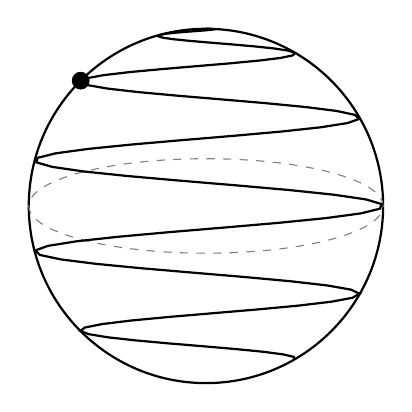
\begin{tikzpicture}[scale=1.5]
        % --- 1. Esfera (Contorno) ---
        \draw[thick] (0,0) circle (1.5);
        \draw[dashed, gray] (0,0) ellipse (1.5 and 0.4); % Ecuador

        % --- 2. Dibujo de la Espiral (Simulada) ---
        \draw[thick, samples=100, domain=0:10*pi] 
            plot ({1.5*sin(deg(\x/12))*cos(deg(\x))}, {1.5*cos(deg(\x/12))});
            
        % --- 3. Partícula ---
        \filldraw ({1.5*sin(deg(pi/4))*cos(deg(3*pi))}, {1.5*cos(deg(pi/4))}) circle (2pt);
    \end{tikzpicture}
    \caption{Trayectoria espiral sobre una superficie esférica de radio $R$.}
\end{figure}
\subsubsection{Péndulo esférico}

Una partícula $P$ está suspendida de un extremo de una varilla rígida de longitud $L$. La posición se describe con ángulos esféricos $\theta$ y $\phi$ respecto a una base fija $\{E_x, E_y, E_z\}$, donde $E_z$ apunta hacia abajo.

Se pide determinar para un observador fijo al suelo:
\begin{enumerate}
    \item Los marcos de referencia y sistemas de coordenadas.
    \item El vector posición de la partícula $P$.
    \item El vector velocidad angular de la varilla.
    \item Los vectores de velocidad y aceleración de la partícula.
\end{enumerate}

\begin{figure}[!ht]
    \centering
    \begin{tikzpicture}[
        >=Latex, 
        x={(1cm,0cm)}, 
        y={(-0.4cm,-0.3cm)}, % Perspectiva ajustada para claridad
        z={(0cm,-1cm)},      % Eje Z apuntando hacia abajo
        scale=2.5
    ]
        % --- Parámetros ---
        \def\L{2.0}       % Longitud varilla
        \def\thetaAng{35} % Ángulo theta ( plano horizontal)
        \def\phiAng{40}   % Ángulo phi (respecto a la vertical)
        \def\arcRad{0.7}  % Radio para los arcos de ángulo

        % --- Coordenadas ---
        \coordinate (O) at (0,0,0);
        
        % Cálculo de P en coordenadas esféricas (Z hacia abajo)
        \pgfmathsetmacro{\Px}{\L*sin(\phiAng)*cos(\thetaAng)}
        \pgfmathsetmacro{\Py}{\L*sin(\phiAng)*sin(\thetaAng)}
        \pgfmathsetmacro{\Pz}{\L*cos(\phiAng)}
        \coordinate (P) at (\Px, \Py, \Pz);
        \coordinate (Q) at (\Px, \Py, 0); % Proyección en plano XY

        % --- 1. Soporte y Ejes ---
       \begin{scope}[canvas is xy plane at z=0]
            \fill[pattern=north east lines] (0,0) circle (0.15);
            \draw[thick] (0,0) circle (0.15);
        \end{scope}
        \filldraw (O) circle (0.8pt) node[above left] {$O$};

        % Ejes
        \draw[->, thick] (O) -- (1.8,0,0) node[right] {$E_x$};
        \draw[->, thick] (O) -- (0,1.8,0) node[left] {$E_y$};
        \draw[->, thick, -{Latex[length=3mm]}] (O) -- (0,0,2.2) node[below] {$E_z$};

        % --- 2. Proyecciones y Varilla ---
        \draw[dashed, thin, gray!70] (O) -- (Q);
        \draw[dashed, thin, gray!70] (Q) -- (P);
        \draw[dashed, thin, gray!70] (P) -- (0,0,\Pz); % Proyección al eje Z

        % Varilla y Partícula
        \draw[line width=1.5pt, color=gray!70] (O) -- (P) node[midway, right, xshift=2pt] {$L$};
        \filldraw[shading=ball, ball color=gray!40] (P) circle (3pt) node[right, xshift=4pt] {$P$};
        \filldraw[gray] (Q) circle (1pt) node[right] {$Q$};

        % --- 3. Ángulos (CORREGIDOS EN 3D) ---
        
        % Ángulo Theta (Plano XY, es más fácil)
        \draw[->, thin] (\arcRad,0,0) arc (0:\thetaAng:\arcRad);
        \node at ({(\arcRad+0.2)*cos(\thetaAng/2)}, {(\arcRad+0.2)*sin(\thetaAng/2)}, 0) {$\theta$};

        % --- CORRECCIÓN DEL ÁNGULO PHI ---
        % Calculamos 3 puntos en el espacio para dibujar el arco 3D correcto
        % 1. Inicio sobre el eje Ez
        \coordinate (PhiStart) at (0, 0, \arcRad);
        % 2. Fin sobre la varilla OP (P escalado)
        \coordinate (PhiEnd) at ($ (O)!{\arcRad/\L}!(P) $);
        % 3. Un punto intermedio para la curvatura (aprox. a la mitad del ángulo)
        \pgfmathsetmacro{\halfPhi}{\phiAng/2}
        \coordinate (PhiMid) at (
            {\arcRad*sin(\halfPhi)*cos(\thetaAng)},
            {\arcRad*sin(\halfPhi)*sin(\thetaAng)},
            {\arcRad*cos(\halfPhi)}
        );

        % Dibujamos la curva suave pasando por los 3 puntos 3D
        \draw[->, thin] plot [smooth] coordinates {(PhiStart) (PhiMid) (PhiEnd)};
        
        % Etiqueta Phi posicionada cerca del punto medio
        \node at ($(PhiMid) + (0,0,0.2)$) {$\phi$};

    \end{tikzpicture}
    \caption{Esquema del péndulo esférico con la representación correcta del ángulo $\phi$ en el espacio 3D.}
    \label{fig:pendulo_esferico_corregido}
\end{figure}

\newpage
% =========================================================================
% Capítulo 1 - Tema 03: Cinemática en Coordenadas Intrínsecas
% =========================================================================

\section{Tema 3: Cinemática en Coordenadas Intrínsecas}

Las coordenadas intrínsecas (tangencial-normal) describen el movimiento
usando la geometría propia de la trayectoria, sin necesidad de un sistema
de referencia externo fijo.

\subsection{Ejercicios}

% =========================================================================
% Capítulo 1: Cinemática
% Tema 03: Coordenadas intrínsecas
% Problema 01: Árbol de navidad
% =========================================================================
\subsubsection{Árbol de navidad}

Una partícula describe una trayectoria helicoidal cónica, donde el ángulo $\theta$
 representa la posición azimutal de la partícula y $r$ es la distancia radial entre la partícula 
 y el eje vertical. Además, $\beta$ es el ángulo formado entre el vector posición de la partícula 
 y el eje vertical (eje z).

\begin{figure}[!ht]
    \centering
    \begin{tikzpicture}[>=Latex, scale=1.5]
        
        % --- 1. EJES DE REFERENCIA ---
        \draw[->, gray!70] (0,0) -- (3,0) node[anchor=north east]{$x$};
        \draw[->, gray!70] (0,0) -- (0,4) node[anchor=south]{$z$};
        % Eje Y en perspectiva
        \draw[->, gray!70] (0,0) -- (-1.2,-1) node[anchor=north east]{$y$};

        % --- 2. PARÁMETROS DE LA ESPIRAL ---
        % Radio aumenta con la altura (z = k * r)
        % x = z * tan(beta) * cos(theta)
        % y = z * tan(beta) * sin(theta)
        \def\betaAng{30} % Ángulo del cono (beta)
        \def\k{0.57}      % tan(30°) aprox.
        
        % --- 3. LÍNEA GENERATRIZ DEL CONO ---
        \draw[thick] (0,0) -- ({3*\k}, 3.5) node[right, pos=0.8] {Generatriz};

        % --- 4. ESPIRAL CÓNICA (Trayectoria) ---
        % Dibujamos 4 vueltas (domain=0:8*pi)
        \draw[thick, blue!80!black] plot[domain=0:25, samples=200, variable=\t]
            ({0.1*\t * \k * cos(\t r) - 0.05*\t * \k * sin(\t r)}, 
             {0.13*\t}); 
             % Nota: El término negativo en x simula la inclinación del eje y

        % --- 5. PUNTO P ---
        % Elegimos un punto arbitrario en la espiral (t=14)
        \coordinate (P) at ({1.4 * \k * cos(14 r) - 0.7 * \k * sin(14 r)}, {1.4*1.3});
        \filldraw (P) circle (1.5pt) node[left, yshift=-4pt] {$P$};

        % --- 6. ÁNGULOS ---
        % Ángulo Beta (entre eje Z y generatriz)
        \draw[->, thick] (0,2) arc (90:65:2);
        \node at (0.35, 1.8) {$\beta$};

        % Ángulo Theta (azimutal en la base)
        % Dibujamos la proyección en el "suelo"
        \draw[dashed, gray] (0,0) -- (-0.85, -0.6);
        \draw[->, thick] (0.8, 0) arc (0:-125:0.8 and 0.4);
        \node at (-0.5, -0.8) {$\theta$};

    \end{tikzpicture}
    \caption{Trayectoria de una partícula $P$ que se desplaza sobre una superficie cónica. Se muestran las coordenadas angulares $\beta$ (polar) y $\theta$ (azimutal).}
    \label{fig:espiral_conica}
\end{figure}
 se conoce que $\dot{r}=c$ y $\theta= \dfrac{2\pi r}{R}$
\begin{enumerate}
    \item Defina marcos de referencia y sistemas de coordenadas.
    \item Determine la posición de $P$ según un observador fijo. 
    \item Determine la  velocidad y aceleración de $P$ según un observador fijo en el marco de referencia inercial. 
\end{enumerate}

% --- SOLUCIÓN ---------------------------------------------------------------
\begin{solucion}{Árbol de navidad}
\textbf{Defina marcos de referencia y sistemas de coordenadas.}
 \textbf{Respuesta:} Los marcos de referencia en este problema son:
    \begin{itemize}
        \item $\mathcal{N}$: Suelo (inercial).
        \item $\mathcal{A}$: Proyeccion del punto P sobre el plano XY con el centro.
    \end{itemize}
                Por otra parte, se definen los siguientes sistemas de coordenadas orto normales:
            \begin{itemize}
                \item $\{ \vec{e}_x, \vec{e}_y, \vec{e}_z \}$: Fijo en $\mathcal{N}$.
                \item $\{ \vec{e}_r, \vec{e}_{\theta}, \vec{e}_z \}$: Fijo en $\mathcal{A}$.
            \end{itemize}

\textbf{Determine la posición de $P$ según un observador fijo. }
\begin{center}
    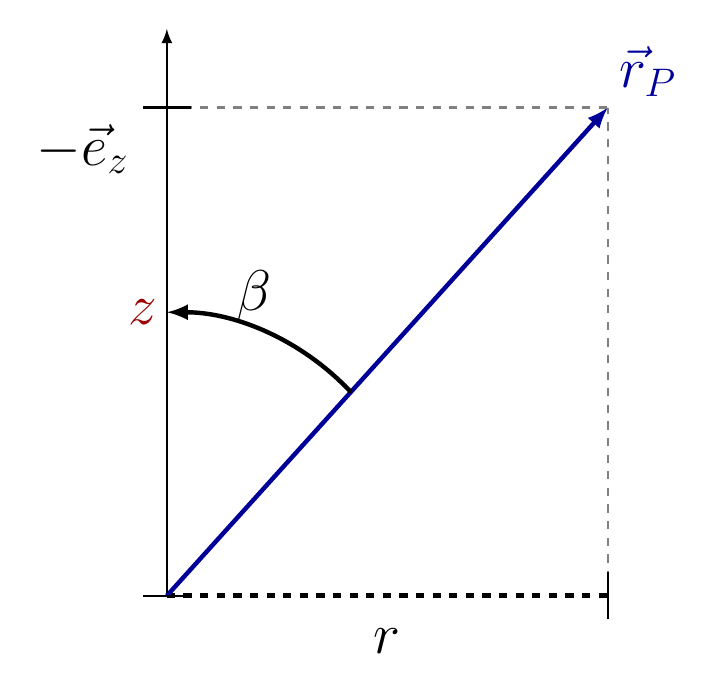
\begin{tikzpicture}
        % Vertical axis (solid) and horizontal axis (dashed)
        \draw[thick, -latex] (0, 0) -- (0, 7.2) node[anchor=north east, pos=0.85, xshift=-10pt] {\huge $-\vec{e}_z$};
        \draw[dashed, ultra thick] (0, 0) -- (5.6, 0);
        
        % Vector r_P
        \draw[ultra thick, blue!60!black, -latex] (0, 0) -- (5.6, 6.2) node[anchor=south west] {\huge $\vec{r}_P$};
        
        % Projected lines (dotted)
        \draw[dashed, thick, gray] (5.6, 0) -- (5.6, 6.2);
        \draw[dashed, thick, gray] (0, 6.2) -- (5.6, 6.2);
        
        % Labels
        \node[red!60!black, anchor=east] at (0, 3.6) {\huge $z$};
        \node[anchor=north] at (2.8, -0.3) {\huge $r$};
        
        % Ticks
        \draw[thick] (-0.3, 0) -- (0.3, 0);
        \draw[thick] (-0.3, 6.2) -- (0.3, 6.2);
        \draw[thick] (5.6, -0.3) -- (5.6, 0.3);
        
        % Angle arc
        \draw[ultra thick, black, latex-] (0, 3.6) arc [start angle=90, end angle=43, radius=3.2] node[midway, anchor=south, xshift=-5pt] {\huge $\beta$};
    \end{tikzpicture}
\end{center}
\textbf{Respuesta:} Notemos que, por geometría, la altura de la partícula está dada por
        \begin{equation}
            z = \frac{r}{\tan (\beta)}.
        \end{equation}
        
        Por lo tanto, la posición de la partícula puede describirse en coordenadas cilíndricas como
        \begin{align}
            \vec{r}_P &= r\vec{e}_{r} - z\vec{e}_z \\
                &= r\vec{e}_{r} - \frac{r}{\tan (\beta)} \vec{e}_z .
        \end{align}
Y de las relaciones se conoce que $\dot\theta=\dfrac{2\pi c}{R}$


       

\textbf{Determine la  velocidad y aceleración de $P$ según un observador fijo en el marco de referencia inercial.}



 Aplicando el Teorema de Transporte, la velocidad de $P$ nos queda:
        \begin{align*}
            \leftidx{^{\mathcal{N}}}{\vec{v}}{_P} = \leftidx{^{\mathcal{N}}}{\frac{d}{dt}}{} \left( \vec{r}_P \right) &=  \leftidx{^{\mathcal{A}}}{\frac{d}{dt}}{} \left( \vec{r}_P \right) + \leftidx{^{\mathcal{N}}}{\vec{\omega}}{^{\mathcal{A}}} \times \vec{r}_P \\
                &= \dot{r}\vec{e}_{r} - \frac{\dot{r}}{\tan (\beta)} \vec{e}_z + \dot{\theta} \vec{e}_z \times \left( r\vec{e}_{r} - \frac{r}{\tan (\beta)} \vec{e}_z \right) \\
                &= \dot{r}\vec{e}_{r} + r\dot{\theta} \vec{e}_{\theta} - \frac{\dot{r}}{\tan (\beta)} \vec{e}_z .\\
                &= c\vec{e}_{r} + r\dfrac{2\pi c}{R} \vec{e}_{\theta} - \frac{c}{\tan (\beta)} \vec{e}_z .
        \end{align*}

        Para obtener la aceleración podemos aplicar nuevamente Teorema de Transporte:
        \begin{align}
            \leftidx{^{\mathcal{N}}}{\vec{a}}{_P} = \leftidx{^{\mathcal{N}}}{\frac{d}{dt}}{} \left( \leftidx{^{\mathcal{N}}}{\vec{v}}{_P} \right) &= \leftidx{^{\mathcal{A}}}{\frac{d}{dt}}{} \left( \leftidx{^{\mathcal{N}}}{\vec{v}}{_P} \right) + \leftidx{^{\mathcal{N}}}{\vec{\omega}}{^{\mathcal{A}}} \times \leftidx{^{\mathcal{N}}}{\vec{v}}{_P} \\
                &= \ddot{r}\vec{e}_{r} + \left( \dot{r}\dot{\theta} + r\ddot{\theta} \right) \vec{e}_{\theta} - \frac{\ddot{r}}{\tan (\beta)} \vec{e}_z + \dot{\theta} \vec{e}_z \times \left( \dot{r}\vec{e}_{r} + r\dot{\theta} \vec{e}_{\theta} - \frac{\dot{r}}{\tan (\beta)} \vec{e}_z \right) \\
                &= \ddot{r}\vec{e}_{r} + \left( \dot{r}\dot{\theta} + r\ddot{\theta} \right) \vec{e}_{\theta} - \frac{\ddot{r}}{\tan (\beta)} \vec{e}_z + \dot{r}\dot{\theta}\vec{e}_{\theta} - r\dot{\theta}^2 \vec{e}_{r} \\
                &= \left( \ddot{r} - r\dot{\theta}^2 \right) \vec{e}_r + \left( 2\dot{r}\dot{\theta} + r\ddot{\theta} \right) \vec{e}_{\theta} - \frac{\ddot{r}}{\tan (\beta)} \vec{e}_z .
        \end{align}
        A su vez se conoce que $\dot{r}=c$ por ende $\ddot{r}=0$ y que $\dot\theta=\dfrac{2\pi c}{R}$ asi mismo  $\ddot\theta=0$

                \begin{equation}
             \leftidx{^{\mathcal{N}}}{\vec{a}}{_P}=\left(-r\left(\dfrac{2\pi c}{R}\right)^2\right)\vec{e}_r+\left(2c\dfrac{2\pi c}{R}\right)\vec{e}_{\theta}
        \end{equation}
\end{solucion}


% --- SOLUCIÓN ---------------------------------------------------------------
\begin{solucion}{Árbol de navidad (sin condición sobre $R$ y $\theta$)}
\vspace{0.8em}
\noindent\textbf{1. Definición de marcos de referencia y sistemas de coordenadas}

Para abordar el problema, identificamos los siguientes marcos de referencia:
\begin{itemize}
    \item $\mathcal{N}$: Marco de referencia inercial asociado al suelo.
    \item $\mathcal{A}$: Marco de referencia no inercial (imaginario) que gira de manera solidaria con el incremento del ángulo azimutal $\theta$.
\end{itemize}

Asimismo, definimos dos sistemas de coordenadas ortonormales para describir el movimiento:
\begin{itemize}
    \item $\{ \vec{e}_x, \vec{e}_y, \vec{e}_z \}$: Sistema fijo en el marco inercial $\mathcal{N}$.
    \item $\{ \vec{e}_r, \vec{e}_{\theta}, \vec{e}_z \}$: Sistema cilíndrico fijo en el marco móvil $\mathcal{A}$.
\end{itemize}

\vspace{0.8em}
\noindent\textbf{2. Posición, velocidad y aceleración de la partícula}

\textbf{pregunta sin puntaje} Determine la posición, velocidad y aceleración de $P$ según un observador fijo en el marco de referencia inercial.

\paragraph{Posición:} A partir de la geometría del cono, la altura $z$ de la partícula se relaciona con el radio $r$ mediante la constante $\beta$:
\[
    z = \frac{r}{\tan(\beta)}.
\]
De este modo, expresamos el vector de posición de $P$ en coordenadas cilíndricas como:
\begin{align*}
    \vec{r}_P &= r\vec{e}_{r} - z\vec{e}_z \\
              &= r\vec{e}_{r} - \frac{r}{\tan(\beta)} \vec{e}_z.
\end{align*}

\paragraph{Velocidad:} Para calcular la velocidad desde el marco inercial $\mathcal{N}$, derivamos la posición empleando el Teorema de Transporte:
\begin{align*}
    \leftidx{^{\mathcal{N}}}{\vec{v}}{_P} &= \leftidx{^{\mathcal{N}}}{\frac{d}{dt}}{} \left( \vec{r}_P \right) = \leftidx{^{\mathcal{A}}}{\frac{d}{dt}}{} \left( \vec{r}_P \right) + \leftidx{^{\mathcal{N}}}{\vec{\omega}}{^{\mathcal{A}}} \times \vec{r}_P \\
    &= \left( \dot{r}\vec{e}_{r} - \frac{\dot{r}}{\tan(\beta)} \vec{e}_z \right) + \left( \dot{\theta} \vec{e}_z \right) \times \left( r\vec{e}_{r} - \frac{r}{\tan(\beta)} \vec{e}_z \right) \\
    &= \dot{r}\vec{e}_{r} + r\dot{\theta} \vec{e}_{\theta} - \frac{\dot{r}}{\tan(\beta)} \vec{e}_z.
\end{align*}

\paragraph{Aceleración:} Aplicamos nuevamente el Teorema de Transporte sobre el vector velocidad:
\begin{align*}
    \leftidx{^{\mathcal{N}}}{\vec{a}}{_P} &= \leftidx{^{\mathcal{N}}}{\frac{d}{dt}}{} \left( \leftidx{^{\mathcal{N}}}{\vec{v}}{_P} \right) = \leftidx{^{\mathcal{A}}}{\frac{d}{dt}}{} \left( \leftidx{^{\mathcal{N}}}{\vec{v}}{_P} \right) + \leftidx{^{\mathcal{N}}}{\vec{\omega}}{^{\mathcal{A}}} \times \leftidx{^{\mathcal{N}}}{\vec{v}}{_P} \\
    &= \left( \ddot{r}\vec{e}_{r} + (\dot{r}\dot{\theta} + r\ddot{\theta})\vec{e}_{\theta} - \frac{\ddot{r}}{\tan(\beta)}\vec{e}_z \right) + \dot{\theta}\vec{e}_z \times \left( \dot{r}\vec{e}_{r} + r\dot{\theta}\vec{e}_{\theta} - \frac{\dot{r}}{\tan(\beta)}\vec{e}_z \right) \\
    &= \left( \ddot{r} - r\dot{\theta}^2 \right)\vec{e}_r + \left( 2\dot{r}\dot{\theta} + r\ddot{\theta} \right)\vec{e}_{\theta} - \frac{\ddot{r}}{\tan(\beta)}\vec{e}_z.
\end{align*}
Dado que la rapidez radial es constante ($\dot{r} = c$), su derivada temporal es nula ($\ddot{r} = 0$). Sustituyendo esta condición, la aceleración simplificada resulta:
\[
    \leftidx{^{\mathcal{N}}}{\vec{a}}{_P} = (-r\dot{\theta}^2)\vec{e}_r + (2c\dot{\theta} + r\ddot{\theta})\vec{e}_{\theta}.
\]

\vspace{0.8em}
\noindent\textbf{3. Distancia radial en el punto $Q$ donde la rapidez es $3c$}

Primero, determinamos la norma del vector velocidad en cualquier instante:
\begin{align*}
    \leftidx{^{\mathcal{N}}}{v}{_P} := \| \leftidx{^{\mathcal{N}}}{\vec{v}}{_P} \| &= \sqrt{ \dot{r}^2 + r^2\dot{\theta}^2 + \left( -\frac{\dot{r}}{\tan(\beta)} \right)^2 }.
\end{align*}
Evaluando la condición $\leftidx{^{\mathcal{N}}}{v}{_P} = 3c$ para el punto $Q$ (usando $\dot{r} = c$):
\begin{align*}
    \sqrt{ c^2 + r^2\dot{\theta}^2 + \left( \frac{c}{\tan(\beta)} \right)^2 } &= 3c \\
    \Leftrightarrow c^2 + r^2\dot{\theta}^2 + \frac{c^2}{\tan^2(\beta)} &= 9c^2 \\
    \Leftrightarrow r^2\dot{\theta}^2 &= c^2 \left( 8 - \frac{1}{\tan^2(\beta)} \right).
\end{align*}
Despejando el radio $r$, encontramos la distancia radial en $Q$:
\begin{align*}
    r = \frac{c}{\dot{\theta}} \sqrt{8 - \frac{1}{\tan^2(\beta)}}.
\end{align*}

\vspace{0.8em}
\noindent\textbf{4. Radio de curvatura en el punto $Q$}



El radio de curvatura $R$ se define conceptualmente a través de la rapidez y la magnitud de la derivada del vector unitario tangente $\vec{e}_t$:
\[
    R = \frac{1}{\kappa} = \frac{\leftidx{^{\mathcal{N}}}{v}{_P}}{\left\| \leftidx{^{\mathcal{N}}}{\frac{d}{dt}}{} (\vec{e}_t) \right\|}.
\]
Construimos el vector tangente unitario usando la relación $\cot(\beta) = \frac{1}{\tan(\beta)}$:
\begin{align*}
    \vec{e}_t = \frac{c\vec{e}_r + r\dot{\theta}\vec{e}_{\theta} - c\cot(\beta)\vec{e}_z}{\sqrt{c^2(1+\cot^2(\beta)) + (r\dot{\theta})^2}}.
\end{align*}
Derivamos el vector $\vec{e}_t$ con respecto al tiempo dividiendo el proceso por la regla del producto:
\begin{align*}
    \leftidx{^{\mathcal{N}}}{\frac{d}{dt}}{} \left( c\vec{e}_r + r\dot{\theta}\vec{e}_\theta - c\cot(\beta)\vec{e}_z \right) &= -r\dot{\theta}^2\vec{e}_r + (2c\dot{\theta} + r\ddot{\theta})\vec{e}_{\theta}, \\
    \leftidx{^{\mathcal{N}}}{\frac{d}{dt}}{} \left( \frac{1}{\sqrt{c^2(1+\cot^2(\beta)) + (r\dot{\theta})^2}} \right) &= -\frac{r\dot{\theta}(r\ddot{\theta} + c\dot{\theta})}{\left(c^2(\cot^2(\beta)+1) + (r\dot{\theta})^2\right)^{3/2}}.
\end{align*}

Evaluando la norma del denominador en el punto $Q$ (donde la norma de la velocidad vale $3c$):
\[
    \sqrt{c^2(1+\cot^2(\beta)) + (r\dot{\theta})^2} = 3c.
\]
Sustituyendo y agrupando componentes en $\vec{e}_r$, $\vec{e}_\theta$ y $\vec{e}_z$:
\begin{align*}
    \left\| \leftidx{^{\mathcal{N}}}{\frac{d}{dt}}{} (\vec{e}_t) \right\| &= \frac{1}{(3c)^3} \left\| -(r\dot{\theta}^2(3c)^2 + c r\dot{\theta}(r\ddot{\theta}+c\dot{\theta}))\vec{e}_r + ((2c\dot{\theta}+r\ddot{\theta})(3c)^2 - (r\dot{\theta})^2(r\ddot{\theta}+c\dot{\theta}))\vec{e}_{\theta} + c\cot(\beta)r\dot{\theta}(r\ddot{\theta}+c\dot{\theta})\vec{e}_z \right\| \\
    &= \frac{1}{(3c)^3} \sqrt{ (r\dot{\theta})^2 \left( (\dot{\theta}(3c)^2 + c(r\ddot{\theta}+c\dot{\theta}))^2 + (c\cot(\beta)(r\ddot{\theta}+c\dot{\theta}))^2 \right) + \left( (2c\dot{\theta}+r\ddot{\theta})(3c)^2 - (r\dot{\theta})^2(r\ddot{\theta}+c\dot{\theta}) \right)^2 }.
\end{align*}
Finalmente, utilizando $v_P = 3c$, el radio de curvatura en $Q$ resulta:
\[
    R = \frac{(3c) \cdot (3c)^3}{\sqrt{ (r\dot{\theta})^2 \left( (\dot{\theta}(3c)^2 + c(r\ddot{\theta}+c\dot{\theta}))^2 + (c\cot(\beta)(r\ddot{\theta}+c\dot{\theta}))^2 \right) + \left( (2c\dot{\theta}+r\ddot{\theta})(3c)^2 - (r\dot{\theta})^2(r\ddot{\theta}+c\dot{\theta}) \right)^2 }}.
\]

\vspace{0.8em}
\noindent\textbf{5. Longitud de arco recorrida hasta el punto $Q$}

\textbf{pregunta sin puntaje} Encuentre una expresión para la longitud de arco recorrida por la partícula desde que parte en el vértice de la espiral hasta que alcanza el punto $Q$.

Por definición, la longitud de arco recorrida $s(t^*)$ desde el reposo/vértice ($t_0 = 0$, $s(0) = 0$) corresponde a la integral temporal de la rapidez:
\[
    s(t^*) = \int_{0}^{t^*} \leftidx{^{\mathcal{N}}}{v}{_P} \, dt = \int_{0}^{t^*} \sqrt{ c^2 + (ct)^2\dot{\theta}^2 + \left( -\frac{c}{\tan(\beta)} \right)^2 } \, dt,
\]
donde hemos utilizado $r(t) = c \cdot t$.

Para determinar el límite superior de integración $t^*$, tomamos la relación obtenida en el punto $Q$:
\[
    r\dot{\theta} = c \sqrt{8 - \frac{1}{\tan^2(\beta)}} \implies t^* \dot{\theta} = \sqrt{8 - \frac{1}{\tan^2(\beta)}}.
\]
Definiendo una función auxiliar $g(t) = t \cdot \dot{\theta}(t)$, podemos despejar el tiempo $t^*$ mediante su función inversa:
\[
    t^* = g^{-1}\left( \sqrt{8 - \frac{1}{\tan^2(\beta)}} \right).
\]
Sustituyendo el límite de integración, la expresión final para la longitud de arco es:
\[
    s(t^*) = \int_{0}^{g^{-1}\left( \sqrt{8 - \frac{1}{\tan^2(\beta)}} \right)} \sqrt{ c^2 + (ct)^2\dot{\theta}^2 + \left( -\frac{c}{\tan(\beta)} \right)^2 } \, dt.
\]
\end{solucion}


\clearpage
\subsubsection{Partícula en cardioide}
Una partícula se mueve a lo largo de una trayectoria con forma de cardioide como se muestra en la Figura \ref{fig:cardioide}. La ecuación de la cardioide es
\[ r = a(1 - \cos \theta) \]
donde \( \theta \) es el ángulo medido desde la dirección horizontal fija. Suponiendo que \( \theta \in [0, \pi] \), determine las siguientes magnitudes relativas a un observador en un sistema de referencia fijo:

\begin{enumerate}
    \item El parámetro de longitud de arco \( s \) como función del ángulo \( \theta \).
    \item La base intrínseca \( \{ \vec{e}_t, \vec{e}_n, \vec{e}_b \} \) y la curvatura de la trayectoria como función del ángulo \( \theta \).
    \item La posición, velocidad y aceleración de la partícula en términos de la base intrínseca \( \{ \vec{e}_t, \vec{e}_n, \vec{e}_b \} \).
\end{enumerate}

\begin{figure}[!ht]
    \centering
    \begin{tikzpicture}[>=Latex, scale=1.8]
        % --- Parámetros Geométricos ---
        \def\a{1.2}      % Escala de la cardioide
        \def\angP{100}    % Ángulo para posicionar el punto P

        % --- 1. Trayectoria Cardioide con sombreado ---
        \shadedraw[inner color=gray!5, outer color=gray!40, line width=0.8pt, domain=0:360, samples=200, smooth, variable=\t] 
            plot ({\t}: {\a*(1-cos(\t))});

        % --- 2. Ejes y Referencia ---
        \coordinate (O) at (0,0);
        \draw[thick] (O) -- (1.5,0); % Eje horizontal de referencia
        \filldraw (O) circle (1.5pt) node[below left] {$O$};

        % --- 3. Punto P y Vector Posición ---
        % Cálculo de la posición de P en coordenadas polares
        \coordinate (P) at ({\angP}: {\a*(1-cos(\angP))});
        
        \draw[->, thick] (O) -- (P) node[midway, left, yshift=2pt] {$r$};
        \filldraw (P) circle (1.5pt) node[above left] {$P$};

        % --- 4. Representación del Ángulo Theta ---
        \draw[->] (0.5,0) arc (0:\angP:0.5);
        \node at (0.25, 0.15) {$\theta$};

    \end{tikzpicture}
    \caption{Partícula moviéndose en una trayectoria con forma de cardioide definida por la ecuación $r = a(1 - \cos \theta)$.}
    \label{fig:cardioide}
\end{figure}
\clearpage
% =========================================================================
% Capítulo 1: Cinemática
% Tema 03: Coordenadas intrínsecas
% Problema 03: Sistema pistón-biela-cigüeñal
% =========================================================================
\subsubsection{Sistema pistón-biela-cigüeñal}

El punto de unión $P$ entre un pistón y una biela de longitud $D$ se mueve a lo largo del eje horizontal $\vec{e}_x$ debido a que el cigüeñal (representado por un disco), de radio $R$ y centro en un punto fijo $O$, rota a una velocidad angular constante $\omega$. En el instante $t=0$, la biela se encuentra en posición horizontal ($\phi = 0$ y $x = R + D$). Realice lo siguiente:

\begin{enumerate}
    \item Identifique los marcos de referencia y defina los sistemas de coordenadas adecuados para describir el movimiento.
    \item Encuentre una expresión para el vector posición $\vec{r}_P$ del pistón medido desde el punto $O$ en función del ángulo $\phi$.
    \item Determine los vectores de velocidad angular y aceleración angular de la biela $AP$.
    \item Calcule los vectores de velocidad y aceleración del pistón $P$.
    \item Determine la distancia total (longitud de arco) recorrida por el pistón $P$ tras una vuelta completa del cigüeñal.
\end{enumerate}

\begin{figure}[!ht]
    \centering
    \begin{tikzpicture}[>=Latex, scale=1.6]
        % --- Parámetros Geométricos ---
        \def\R{1.2}      % Radio del cigüeñal
        \def\D{3.5}      % Longitud de la biela
        \def\phiAng{50}  % Ángulo de giro phi
        \def\BarThick{0.06} % Grosor de las barras

        % --- Coordenadas ---
        \coordinate (O) at (0,0);
        \coordinate (A) at (\phiAng:\R);
        % Posición x del pistón calculada por trigonometría: R*cos(phi) + sqrt(D^2 - (R*sin(phi))^2)
        \pgfmathsetmacro{\Px}{\R*cos(\phiAng) + sqrt(\D*\D - (\R*sin(\phiAng))^2)}
        \coordinate (P) at (\Px, 0);

        % --- 1. Cigüeñal (Disco y Eje) ---
        \draw[dashed, thin] (O) circle (\R);
        \draw[thick] (-0.2,0) -- (6.0,0); % Eje de guía x
        
        % Velocidad angular omega
        \draw[->, thick] (0.5, 0.8) arc (40:140:0.6);
        \node[below] at (0, 0.8) {$\omega$};

        % --- 2. Barra OA (Cigüeñal) ---
        \begin{scope}[rotate=\phiAng]
            \shadedraw[inner color=white, outer color=gray!40, draw=black, rounded corners=2pt] 
                (-0.1, -\BarThick) rectangle ({\R+0.1}, \BarThick);
        \end{scope}
        \node[above left] at ($(O)!0.5!(A)$) {$R$};

        % --- 3. Barra AP (Biela) ---
        % Ángulo de la biela con la horizontal (beta)
        \pgfmathsetmacro{\betaAng}{asin(\R*sin(\phiAng)/\D)}
        \begin{scope}[shift={(A)}, rotate=-\betaAng]
            \shadedraw[inner color=white, outer color=gray!40, draw=black, rounded corners=2pt] 
                (-0.1, -\BarThick) rectangle ({\D+0.1}, \BarThick);
        \end{scope}
        \node[above] at ($(A)!0.5!(P)$) {$D$};

        % --- 4. El Pistón (P) ---
        \shadedraw[top color=gray!10, bottom color=gray!80, draw=black, thick] 
            ($ (P) + (-0.2, -0.15) $) rectangle ($ (P) + (0.2, 0.15) $);
        
        % --- 5. Articulaciones (Gris oscuro) ---
        \filldraw[fill=gray!80, draw=black] (O) circle (1.8pt) node[below left] {$O$};
        \filldraw[fill=gray!80, draw=black] (A) circle (1.8pt) node[above right] {$A$};
        \filldraw[fill=gray!80, draw=black] (P) circle (1.2pt) node[above right, yshift=2pt] {$P$};

        % --- 6. Cotas y Referencias ---
        % Ángulo phi
        \draw[dashed] (O) -- (1.5,0);
        \draw[->] (0.7,0) arc (0:\phiAng:0.7);
        \node at (0.9, 0.25) {$\phi$};

        % Cota de distancia x
        \draw[<->] (0,-0.4) -- (\Px,-0.4) node[midway, fill=white] {$x$};
        \draw[dotted] (0,0) -- (0,-0.5);
        \draw[dotted] (\Px,0) -- (\Px,-0.5);

    \end{tikzpicture}
        \caption{Esquema cinemático de un mecanismo de pistón accionado por un cigüeñal de radio $R$ y biela de longitud $D$.}
    \label{fig:piston_biela}
\end{figure}
\clearpage

\newpage
% =========================================================================
% Capítulo 1 - Tema 04: Rodadura sin Deslizar
% =========================================================================

\section{Tema 04: Rodadura sin Deslizar}

La restricción de rodadura sin deslizar relaciona la velocidad de traslación
del centro de un cuerpo con su velocidad angular, y es fundamental para
analizar discos, ruedas y cilindros en contacto con una superficie.

\subsection{Ejercicios}

\subsubsection{Barra pelota}
Un brazo de longitud \( l \) está articulado en uno de sus extremos al centro de un disco circular de radio \( r \), como se muestra en la Figura \ref{fig:rodadura_varilla}. El disco rueda sin deslizamiento a lo largo de una superficie horizontal fija. Usando la variable \( x \) para describir la posición del centro del disco y la variable \( \phi \) para describir la orientación del brazo con respecto a la vertical, determine los siguientes vectores según lo visto por un observador fijo al suelo:

\begin{enumerate}
    \item La velocidad y aceleración del centro del disco.
    \item La velocidad y aceleración angular del disco
    \item La velocidad y aceleración del extremo libre del brazo.
\end{enumerate}
\begin{figure}[!ht]
    \centering
    \begin{tikzpicture}[>=Latex, scale=1.8]
        % --- Parámetros Geométricos ---
        \def\R{1.5}      % Radio del cilindro
        \def\L{2.2}      % Longitud de la varilla l
        \def\PhiAng{30}  % Ángulo phi respecto a la vertical

        % --- 1. Suelo (Superficie de rodadura) ---
        \draw[thick] (-2,0) -- (3.5,0);
        \fill[pattern=north east lines, pattern color=gray!60] (-2, -0.2) rectangle (3.5, 0);

        % --- 2. Cilindro ---
        \coordinate (O) at (0, \R); % Centro O
        \coordinate (Q) at (0, 0);  % Punto de contacto Q
        
        % Sombreado degradado para el cilindro
        \shadedraw[inner color=gray!10, outer color=gray!70] (O) circle (\R);
        \filldraw (O) circle (1.5pt) node[above left] {$O$};
        \filldraw (Q) circle (1pt) node[above left, xshift=-2pt] {$Q$};

        % --- 3. Ejes y Referencias ---
        % Eje x desde el centro
        \draw[->, thick] (O) -- (2.5, \R) node[below] {$x$};
        % Línea vertical discontinua
        \draw[dashed, gray] (O) -- (0, -0.5);
        % Radio R
        \draw[->, thick] (O) -- ({\R*cos(45)}, {\R+\R*sin(45)}) node[midway, above left] {$R$};

        % --- 4. Varilla acoplada en O ---
        % Punto P al final de la varilla
        \coordinate (P) at ({\L*sin(\PhiAng)}, {\R - \L*cos(\PhiAng)});
        
        % Varilla con grosor (estilo 2D)
        \draw[line width=6pt, line cap=round, color=black] (O) -- (P);
        \draw[line width=5pt, line cap=round, color=gray!50!white] (O) -- (P);
        \draw[thick] (O) -- (P);
        \filldraw (P) circle (1pt) node[below right] {$P$};
        \node[right, xshift=3pt] at ($(O)!0.5!(P)$) {$l$};

        % --- 5. Ángulo Phi ---
        \draw[->] (0, 0.5) arc (-90:{-90+\PhiAng}:0.8);
        \node at (0.3, 0.4) {$\phi$};

        % --- 6. Indicación "No desliza" ---
        \coordinate (NoSlipPoint) at (-0.8, 0.2);
        \node[left] at (-1, 0.6) {No desliza};
        \draw[thin] (-1, 0.5) to[out=0, in=120] (-0.3, 0.05);

    \end{tikzpicture}
    \caption{Cilindro de radio $R$ rodando sin deslizar sobre una superficie horizontal. Una varilla de longitud $l$ está articulada en el centro $O$, formando un ángulo $\phi$ con la vertical.}
    \label{fig:rodadura_varilla}
\end{figure}
\subsubsection{Rueda de molino}

Una barra de longitud \( L \) con una rueda de radio \( R \) unida a uno de sus extremos está rotando alrededor del eje vertical \( OA \) con una velocidad angular constante \( \Omega \) relativa a un marco de referencia fijo, como se muestra en la Figura~\ref{fig:rueda_brazo_final}. La rueda está vertical y rueda sin deslizamiento a lo largo de una superficie horizontal fija.\\

Determine la velocidad angular y la aceleración angular de la rueda por un observador en un marco de referencia fijo.\\

\begin{figure}[!ht]
    \centering
    % 1. Ajuste de Perspectiva (Ángulo de elevación y azimut)
    \tdplotsetmaincoords{60}{130}

    \begin{tikzpicture}[tdplot_main_coords, scale=1.5, >=Latex]

        % --- Parámetros Ajustados (Proporciones más realistas) ---
        \def\L{3.5}      % Longitud del brazo
        \def\R{1}      % Radio del disco
        \def\Hshaft{2.0} % Altura del eje central
        \def\zO{1}     % Altura de conexión del brazo
        \def\DiskThick{0.2} % Grosor del disco

        % --- 1. Trayectoria Circular en el Suelo ---
        \draw[dashed, gray, thin] (0,0,0) circle (\L);

        % --- 2. Eje Central (Poste) ---
        % Base y tapa para darle solidez
        \def\Raxis{0.4} % Definimos el radio del poste para que sea consistente

        % Cara inferior (Base)

        % Cuerpo del cilindro (Paredes)
        % Dibujamos un rectángulo que une los extremos laterales del círculo
        \draw[fill=gray!30, draw=black,thick](\Raxis+0.1,-0.1,0) arc (-50:130:\Raxis)--++(0,0,\Hshaft)-- ++(0.87,-0.28,0.21)--cycle;
            
        % Cara superior (Tapa)
        \draw[fill=gray!30, thick] (0,0,\Hshaft-0.15) circle (\Raxis);

        % Línea de eje y punto O
        \draw[dash dot, thin] (0,0,-0.5) -- (0,0,\Hshaft + 1.0);
        \coordinate (O) at (0,0,\zO);

        % --- 3. Brazo Rotatorio ---
        \coordinate (B) at (\L, 0, \zO);
        % Línea gruesa y sólida
        \draw[line width=5pt] (O) -- (B) node[midway, above] {$L$};
        \draw[line width=4pt, gray!70, line cap=round] (O) -- (B);

        \filldraw (O) circle (1.5pt) node[left, xshift=-2pt,  yshift=2pt] {$O$};
        % --- 4. Disco en el punto B (Mejorado) ---
        % Rotamos el sistema local para dibujar el disco vertical
        \tdplotsetrotatedcoords{0}{90}{0}
        \begin{scope}[tdplot_rotated_coords, shift={(B)}]
            % Círculo trasero (para dar profundidad)
            \draw[fill=gray!60, thick] (0,0,-\DiskThick) circle (\R);
            
            % Borde del disco (conecta los círculos)
            \draw[thick, gray!60] (0,\R,0) -- (0,\R,-\DiskThick);
            \draw[thick, gray!60] (0,-\R,0) -- (0,-\R,-\DiskThick);

            % Círculo frontal (cara principal)
            \draw[fill=gray!30, thick] (0,0,0) circle (\R);
            
            % Eje del disco
            \draw[fill=gray!80] (0,0,0) circle (0.15);

            % Puntos y Etiquetas
            \filldraw[black] (0,0,0) circle (1.5pt) node[above right] {$B$};
            % Vector Radio R apuntando al suelo
            \draw[->, thick] (0,0,0) -- (0,-\R,0) node[midway, above] {$R$};
        \end{scope}

        % --- 5. Indicador de Rotación Omega ---
        \draw[->, very thick] (0,0,\Hshaft + 0.4) ++(120:0.6) arc (120:420:0.6);
        \node[left] at (-0.6, 0, \Hshaft + 0.7) {$\Omega$};

        % --- Hack para Centrado ---
        % Puntos invisibles extremos para equilibrar la caja delimitadora
        \path (\L+\R, 0, 0); \path (-\L-\R, 0, 0);

    \end{tikzpicture}
    \caption{Representación mejorada del sistema de rueda pivotante. El disco de radio $R$ rueda sobre una trayectoria circular de radio $L$, impulsado por el brazo que gira con velocidad $\Omega$ alrededor del eje vertical.}
    \label{fig:rueda_brazo_final}
\end{figure}
% =========================================================================
% Capítulo 1: Cinemática
% Tema 04: Rodadura sin deslizar
% Problema 03: Disco en pista circular
% =========================================================================
\subsubsection{Disco en pista circular}

Un disco de radio $r$ rueda sin resbalar a lo largo del interior de una pista circular fija de radio $R$ (con $R > r$), como se muestra en la Figura \ref{fig:disco_pista}. El centro de la pista circular se indica con el punto $O$, mientras que el centro del disco se indica con el punto $P$. 

El ángulo $\theta$ se mide desde la dirección fija vertical hacia abajo desde el centro de la pista (dirección $OA$), mientras que el ángulo $\phi$ se mide entre la dirección de la línea $OP$ y la dirección del radio $PQ$, siendo $Q$ un punto en el borde del disco. 

Sabiendo que el punto $Q$ coincide con el punto $A$ (el punto más bajo de la pista) cuando $\theta$ y $\phi$ son cero, determine los siguientes vectores según lo visto por un observador fijo al suelo:

\begin{enumerate}
    \item La velocidad angular $\vec{\omega}$ y la aceleración angular $\vec{\alpha}$ del disco.
    \item La velocidad $\vec{v}_Q$ y aceleración $\vec{a}_Q$ del punto $Q$.
\end{enumerate}

Exprese sus respuestas en términos del ángulo $\phi$ y sus derivadas temporales ($\dot{\phi}, \ddot{\phi}$).

\begin{figure}[!ht]
    \centering
    \begin{tikzpicture}[>=Latex, scale=1.8]
        % --- Parámetros Geométricos ---
        \def\R{2.2}      % Radio de la pista grande
        \def\r{0.7}      % Radio del disco pequeño
        \def\ThetaAng{35} % Ángulo theta de posición del centro P
        \def\PhiAng{65}   % Ángulo phi de rotación del disco

        % --- 1. Pista Circular (Superficie fija) ---
        \coordinate (O) at (0,0);
        \coordinate (A) at (0, -\R);
        
        % Dibujo de la pista con patrón de sombreado exterior

        \fill[pattern=north east lines, pattern color=gray!80] (0,0) circle (\R+0.15) circle (\R);
        \fill[color=white] (0,0) circle (\R) circle (\R);
        \draw[thick] (O) circle (\R);

        % --- 2. Centro del disco P ---
        % El centro P se ubica en una trayectoria circular de radio (R-r)
        \coordinate (P) at ({-90+\ThetaAng}:{\R-\r});
        
        % Líneas de referencia
        \draw[dashed, gray] (O) -- (0, -\R-0.3); % Eje vertical fijo
        \draw[dashed, gray] (O) -- (P);          % Línea OP
        
        % --- 3. Disco rodante ---
        % Sombreado degradado para el disco
        \shadedraw[inner color=gray!5!white, outer color=gray!40] (P) circle (\r);
        \filldraw (P) circle (1.5pt) node[above left, xshift=2pt] {$P$};
        \filldraw (O) circle (1.5pt) node[above] {$O$};
        \node[below] at (A) {$A$};

        % --- 4. Punto Q y ángulo Phi ---
        % El ángulo de Q es relativo a la línea OP (que está a -90+Theta)
        \coordinate (Q) at ($(P) + ({-90+\ThetaAng+\PhiAng}:\r)$);
        \draw[thick] (P) -- (Q);
        \filldraw (Q) circle (1.2pt) node[below right] {$Q$};
        
        % Etiqueta del radio r
        \draw[<->, thin] (P) -- ++(160:\r) node[midway, above] {$r$};
        % Etiqueta del radio R
        \draw[<->, thin] (O) -- (30:\R) node[midway, above left] {$R$};

        % --- 5. Ángulos ---
        % Ángulo Theta (desde la vertical OA hasta OP)
        \draw[->] (0, -0.6) arc (-90:{-90+\ThetaAng}:0.6);
        \node at (-80:0.45) {$\theta$};
        
        % Ángulo Phi (desde la línea OP hasta PQ)
        % Línea de referencia extendida de OP para marcar phi
        \coordinate (RefPhi) at ($(P) + ({-90+\ThetaAng}:0.8)$);
        \draw[dotted, thick] (P) -- (RefPhi);
        \draw[->] ($(P) + ({-90+\ThetaAng}:0.4)$) arc ({-90+\ThetaAng}:{-90+\ThetaAng+\PhiAng}:0.4);
        \node at ($(P) + ({-90+\ThetaAng+0.5*\PhiAng}:0.55)$) {$\phi$};

        % --- 6. Indicación "No desliza" ---
        \node[left] at ({-90+\ThetaAng}: \R+0.6) {No desliza};
        \draw[thin, ->] ({-90+\ThetaAng-10}: \R+0.5) to[out=0, in=120] ({-90+\ThetaAng}: \R+0.05);

    \end{tikzpicture}
    \caption{Disco de radio $r$ rodando sin deslizar por el interior de una pista de radio $R$. El punto $A$ es la referencia vertical inferior.}
    \label{fig:disco_pista}
\end{figure}
% =========================================================================
% Capítulo 1: Cinemática
% Tema 04: Rodadura sin deslizar
% Problema 04: Sistema de dos discos rodantes
% =========================================================================
\subsubsection{Sistema de dos discos rodantes}

Un disco circular de radio $R$ rueda sin resbalar a lo largo de una superficie horizontal fija. Un segundo disco circular de radio $r$ rueda sin resbalar sobre el primer disco. Usando las variables $\theta$ y $\phi$ para describir el movimiento de los discos, determine las siguientes cantidades como las ve un observador en un marco de referencia inercial:

\begin{enumerate}
    \item Velocidad angular y aceleración angular de cada disco.
    \item Velocidad y aceleración del centro de cada disco ($O$ y $C$).
\end{enumerate}

\begin{figure}[!ht]
    \centering
    \begin{tikzpicture}[>=Stealth, scale=1.5]
        % --- Parámetros Geométricos ---
        \def\Rbig{2.0}    % Radio del disco inferior (R)
        \def\Rsmall{1.0}  % Radio del disco superior (r)
        \def\ThetaPos{30} % Ángulo de posición del centro C respecto a la vertical
        \def\PhiPos{40}   % Ángulo interno phi del disco superior

        % --- 1. Suelo Fijo ---
        % Línea base
        \draw[thick] (-3, 0) -- (4, 0);
        % Patrón de sombreado para indicar superficie fija
        \fill[pattern=north east lines, pattern color=gray!50] (-3, -0.3) rectangle (4, 0);

        % --- 2. Disco Inferior (Centro O) ---
        \coordinate (O) at (0, \Rbig);
        % Sombreado radial para efecto 3D
        \shadedraw[inner color=white, outer color=gray!40, thick] (O) circle (\Rbig);
        \filldraw (O) circle (1.5pt) node[left, xshift=-2pt] {$O$};

        % --- 3. Disco Superior (Centro C) ---
        % Calculamos la posición de C basándonos en el ángulo ThetaPos
        \coordinate (C) at ($(O) + ({90-\ThetaPos}:{\Rbig+\Rsmall})$);
        \shadedraw[inner color=white, outer color=gray!40, thick] (C) circle (\Rsmall);
        \filldraw (C) circle (1.5pt) node[above, yshift=2pt] {$C$};

        % --- 4. Punto de Contacto P ---
        \coordinate (P) at ($(O) + ({90-\ThetaPos}:\Rbig)$);
        \filldraw (P) circle (1.2pt) node[right, xshift=3pt] {$P$};

        % --- 5. Líneas de Referencia y Radios ---
        % Línea vertical desde O
        \draw[dashed, gray] (O) -- ++(0, {\Rbig+\Rsmall+1.0});
        % Línea conectando centros OC
        \draw[dashed, gray] (O) -- (C);
        
        % Etiqueta Radio R (disco inferior)
        \draw[->, thin] (O) -- ++(-30:\Rbig) node[midway, below, scale=0.9] {$R$};
        % Etiqueta Radio r (disco superior)
        \draw[->, thin] (C) -- ++({90-\ThetaPos+50}:\Rsmall) node[midway, above right, scale=0.9] {$r$};

        % --- 6. Ángulos ---
        % Ángulo Theta (posición de C respecto a la vertical)
        \draw[->, thick] ($(O)+(0, 1.5)$) arc (90:{90-\ThetaPos}:1.5);
        \node at ($(O)+({90-0.5*\ThetaPos}:1.7)$) {$\phi$};

        % Ángulo Phi (interno en el disco superior)
        % Dibujamos una línea radial de referencia en el disco superior
        \coordinate (CRef) at ($(C) + ({90-\ThetaPos-\PhiPos}:\Rsmall)$);
        \draw[dashed, gray!80] (C) -- (CRef);
        % Arco para phi desde la línea CP hasta CRef
        %\draw[->] ($(C)!0.5!(P)$) arc ({90-\ThetaPos}:{90-\ThetaPos-\PhiPos}:0.5);
        %\node at ($(C)+({90-\ThetaPos-0.5*\PhiPos}:0.7)$) {$ $};

        % --- 7. Flechas de Sentido de Rotación (Decorativas) ---
        % Disco inferior
        \draw[<-, thick, bend right] ($(O)+(-0.6, \Rbig+0.5)$) to node[midway, above] {$\theta$} ($(O)+(-1.5, \Rbig)$);
        % Disco superior
        \draw[<-, thick, bend left] ($(C)+(\Rsmall+0.3, 0.3)$) to ($(C)+(\Rsmall+0.3, -0.3)$);

        % --- 8. Indicación "No Slip" ---
        \node[right] at (3, \Rbig) {Sin deslizamiento};
        % Línea al contacto inferior
        \draw[thin] (3, \Rbig) -- (0,0);
        % Línea al contacto intermedio P
        \draw[thin] (3, \Rbig) -- (P);

    \end{tikzpicture}
    \caption{Sistema de dos discos apilados rodando sin deslizamiento.}
    \label{fig:dos_discos}
\end{figure}

\newpage
% =========================================================================
% Capítulo 1 - Tema 05: Problemas de Mezcla Compleja
% =========================================================================

\section{Tema 05: Problemas de Mezcla Compleja}

Esta sección reúne problemas que combinan múltiples sistemas de coordenadas,
marcos de referencia móviles y restricciones simultáneas, integrando los
conceptos vistos en los temas anteriores.

\subsection{Ejercicios}

% =========================================================================
% Capítulo 1: Cinemática
% Tema 05: Problemas de mezcla compleja
% Problema 01: Disco con brazo pivotante
% =========================================================================
\subsubsection{Disco con brazo pivotante}

Un disco de radio $R$ gira libremente en torno a su centro en un punto ubicado en el extremo de un brazo de longitud $L$, como se muestra en la figura. El mismo brazo pivotea libremente en su otro extremo en el punto $O$ hasta el eje vertical. Finalmente, el eje gira con velocidad angular constante $\Omega$ en relación con el suelo (marco de referencia inercial). Sabiendo que $\phi$ describe la ubicación de un punto $P$ en el borde del disco relativa a la dirección $OQ$ y que $\theta$ se forma entre el brazo y la dirección vertical hacia abajo, determine las siguientes cantidades según las ve un observador fijo al suelo:

\begin{enumerate}
    \item La velocidad angular del disco.
    \item La velocidad y aceleración del punto $P$.
\end{enumerate}

\begin{figure}[!ht]
    \centering
    \begin{tikzpicture}[>=Latex, scale=1.5]
        % --- Parámetros ---
        \def\L{3.0}         % Longitud del brazo L
        \def\Rdisk{1.2}     % Radio del disco R
        \def\thetaang{40}   % Ángulo theta (brazo)
        \def\phiang{55}     % Ángulo phi (punto P)
        \def\ShaftW{0.4}    % Ancho del eje vertical

        % --- 1. Eje Vertical (Soporte) ---
        \fill[pattern=north east lines, pattern color=gray!50] (-\ShaftW-0.2, 0.5) rectangle (-\ShaftW, 2.5);
        \fill[pattern=north east lines, pattern color=gray!50] (\ShaftW, 0.5) rectangle (\ShaftW+0.2, 2.5);
        
        \shadedraw[left color=gray!40, right color=gray!10] (-\ShaftW, 0.5) rectangle (\ShaftW, 2.5);
        \draw[thick] (-\ShaftW, 0.5) -- (-\ShaftW, 2.5);
        \draw[thick] (\ShaftW, 0.5) -- (\ShaftW, 2.5);

        % --- 2. Pivote y Brazo ---
        \coordinate (O) at (0, 1.5);
        \coordinate (Q) at ({\L*sin(\thetaang)}, {1.5 - \L*cos(\thetaang)});
        
        % Línea vertical de referencia
        \draw[dashed, gray] (O) -- (0, -1.5);
        


        % --- 3. Disco en el punto Q ---
        \begin{scope}[shift={(Q)}]
            % Cara del disco
            \shadedraw[inner color=white, outer color=gray!20, thick] (0,0) circle (\Rdisk);
            \filldraw (0,0) circle (1.5pt) node[below right] {$Q$};
        % Brazo L
        \draw[line width=5pt, line cap=round] (O) -- (Q);
        \draw[line width=4pt, gray!30, line cap=round] (O) -- (Q);
        \node[above right] at ($(O)!0.5!(Q)$) {$L$};
        \filldraw (O) circle (1.5pt) node[left, xshift=-2pt] {$O$};            
            % Punto P y radio R
            \coordinate (P) at ({90-\thetaang-\phiang}:\Rdisk);
            \draw[thick, ->] (0,0) -- (P) node[midway, below right] {$R$};
            \filldraw (P) circle (1.5pt) node[above right] {$P$};
            
            % Ángulo phi (respecto a la dirección del brazo OQ)
            \draw[dashed] (0,0) -- ({90-\thetaang}:1.6); % Dirección OQ extendida
            \draw[->] ({90-\thetaang}:0.6) arc ({90-\thetaang}:{90-\thetaang-\phiang}:0.6);
            \node at ({90-\thetaang-0.5*\phiang}:0.8) {$\phi$};
        \end{scope}

        % --- 4. Ángulo theta ---
        \draw[->] (0, 0.7) arc (-90:{-90+\thetaang}:0.8);
        \node at (0.2,0.9) {$\theta$};

        % --- 5. Rotación Omega ---
        \draw[->, ultra thick] (-0.5, 2.8) arc (160:-100:0.5 and 0.15);
        \draw[thick] (0, 2.5) -- (0, 3.0);
        \node[above] at (0, 3.0) {$\Omega$};

    \end{tikzpicture}
    \caption{Esquema 2D del sistema brazo-disco con rotación respecto al eje vertical.}
\end{figure}
\clearpage
% =========================================================================
% Capítulo 1: Cinemática
% Tema 05: Problemas de mezcla compleja
% Problema 02: Barra en aro deslizante
% =========================================================================
\subsubsection{Barra en aro deslizante}

Una barra delgada de longitud $l$ está articulada a un aro como se muestra en la Figura \ref{fig:barra_deslizante}. El aro se desliza libremente a lo largo de una pista horizontal fija. Si se sabe que $x$ es el desplazamiento horizontal del aro y que $\theta$ describe la orientación de la barra en relación con la dirección vertical, determine las siguientes magnitudes según las ve un observador fijo en la pista (marco de referencia inercial):

\begin{enumerate}
    \item El vector velocidad del extremo libre de la barra (punto $P$).
    \item El vector aceleración del extremo libre de la barra (punto $P$).
\end{enumerate}

\begin{figure}[!ht]
    \centering
    \begin{tikzpicture}[>=Latex, scale=1.5]
        % --- Parámetros ---
        \def\L{2.5}         % Longitud de la barra l
        \def\ThetaAng{45}   % Ángulo theta
        \def\TrackW{5.0}    % Ancho de la pista

        % --- 1. Pista Horizontal (Fija) ---
        % Sombreado de los extremos fijos
        \fill[pattern=north east lines, pattern color=gray!60] (-2.5, -0.3) rectangle (-2.3, 0.3);
        \draw[-,thick] (-2.3,-0.3)--++(0,0.6);
        \fill[pattern=north east lines, pattern color=gray!60] (2.3, -0.3) rectangle (2.5, 0.3);
        \draw[-,thick] (2.3,-0.3)--++(0,0.6);
        
        % Cuerpo de la pista (dos líneas paralelas para dar volumen)
        \draw[thick, fill=gray!10] (-2.3, -0.08) rectangle (2.3, 0.08);

        % --- 2. Aro Deslizante (Punto O) ---
        \coordinate (O) at (0,0);
        \shadedraw[inner color=white, outer color=gray!60, rounded corners=2pt] (-0.2,-0.15) rectangle (0.2,0.15);
        \filldraw (O) circle (1.5pt) node[below left, yshift=-2pt] {$O$};

        % --- 3. Barra delgada (Punto O a P) ---
        \coordinate (P) at ({\L*sin(\ThetaAng)}, {\L*cos(\ThetaAng)});
        
        % Dibujo de la barra con grosor y degradado
        \draw[line width=5pt, line cap=round, black] (O) -- (P);
        \draw[line width=4pt, line cap=round, gray!30] (O) -- (P);
        \node[below right] at ($(O)!0.5!(P)$) {$l$};
        \filldraw (P) circle (0.8pt) node[above right] {$P$};

        % --- 4. Referencias y Ángulo ---
        % Eje vertical de referencia
        \draw[dashed, thick] (O) -- (0, 1.5);
        
        % Arco para el ángulo theta
        \draw[->] (0, 1.0) arc (90:{90-\ThetaAng}:1.0);
        \node at (70:1.2) {$\theta$};

        % --- 5. Indicación de desplazamiento x ---
        \draw[|->, thick] (0, -0.5) -- (1.0, -0.5) node[right] {$x$};

    \end{tikzpicture}
    \caption{Barra de longitud $l$ articulada a un aro que se desplaza horizontalmente una distancia $x$.}
    \label{fig:barra_deslizante}
\end{figure}5

% --- SOLUCIÓN ---------------------------------------------------------------
\begin{solucion}{Barra en aro deslizante (cinemática)}
\textbf{Planteamiento}\\
Hay dos grados de libertad, $x$ y $\theta$. Según la figura la barra está \emph{sobre} el aro y $\theta$ se mide desde la vertical hacia arriba, creciendo en sentido horario: $\theta=0$ es la posición invertida y $\theta=\pi$ la barra colgando.

\patoojo[squareglasses,shovel]{¡Ojo con la figura! La barra apunta hacia \emph{arriba}: $\theta=0$ es la posición invertida (inestable) y $\theta=\pi$ es la barra colgando. Además $\theta$ crece en sentido \emph{horario}, así que $\velang{N}{B}=-\dot\theta\vec{E}_z$.}

\textbf{Marcos de referencia y Sistemas de Coordenadas}
\begin{itemize}
    \item $\mathcal{N}$ La pista (inercial) $\longrightarrow\{\vec{E}_x;\vec{E}_y;\vec{E}_z\}$
    \item $\mathcal{B}$ La barra $\longrightarrow\{\vec{e}_r;\vec{e}_\theta;\vec{E}_z\}$, con $\vec{e}_r$ a lo largo de la barra
\end{itemize}
\begin{equation*}
\begin{split}
    \vec{e}_r&=\sin\theta\,\vec{E}_x+\cos\theta\,\vec{E}_y\\
    \vec{e}_\theta&=\cos\theta\,\vec{E}_x-\sin\theta\,\vec{E}_y
\end{split}
\end{equation*}

\subsubsection*{Cinemática de la partícula}
\textbf{Posición}\\
Tomando como referencia el aro, con $O=(x,0)$ en la pista, el extremo libre $P$ está a una distancia $l$ de $O$ a lo largo de la barra:
$$\vec{r}_P=x\vec{E}_x+l\vec{e}_r=\left(x+l\sin\theta\right)\vec{E}_x+l\cos\theta\,\vec{E}_y$$
Y la velocidad angular de la barra es $\velang{N}{B}=-\dot\theta\vec{E}_z$ (horaria).

\textbf{Velocidad}\\
$$\marc{\vec{v}_P}{N}=\der{\vec{r}_P}{N}=\dot{x}\vec{E}_x+\underbrace{\der{(l\vec{e}_r)}{B}{}}_{\vec{0}}+\velang{N}{B}\times l\vec{e}_r=\dot{x}\vec{E}_x+l\dot\theta\vec{e}_\theta$$
\respuesta{$\displaystyle\marc{\vec{v}_P}{N}=\left(\dot{x}+l\dot\theta\cos\theta\right)\vec{E}_x-l\dot\theta\sin\theta\,\vec{E}_y$}

\textbf{Aceleración}\\
Derivando de nuevo con el teorema del transporte, ahora sobre $\dot{x}\vec{E}_x+l\dot\theta\vec{e}_\theta$:
$$\marc{\vec{a}_P}{N}=\ddot{x}\vec{E}_x+l\ddot\theta\vec{e}_\theta+\velang{N}{B}\times\left(l\dot\theta\vec{e}_\theta\right)=\ddot{x}\vec{E}_x+l\ddot\theta\vec{e}_\theta-l\dot\theta^2\vec{e}_r$$
\respuesta{$\displaystyle\marc{\vec{a}_P}{N}=\left[\ddot{x}+l\left(\ddot\theta\cos\theta-\dot\theta^2\sin\theta\right)\right]\vec{E}_x-l\left(\ddot\theta\sin\theta+\dot\theta^2\cos\theta\right)\vec{E}_y$}

\patotip{Si en cambio piden el centro de masa $G$ de la barra, el cálculo es idéntico reemplazando $l$ por $l/2$ (está a mitad de la barra).}
\end{solucion}

\clearpage
% =========================================================================
% Capítulo 1: Cinemática
% Tema 05: Problemas de mezcla compleja
% Problema 03: Mecanismo de rotación tridimensional
% =========================================================================
\subsubsection{Mecanismo de rotación tridimensional}
Un sistema mecánico consiste en un eje vertical que gira con una velocidad angular $\omega_1$. Unido a este eje en el punto $O$, se encuentra un brazo de longitud $L$ que forma un ángulo $\beta$ con la vertical y gira sobre su propio eje con una velocidad angular $\omega_2$. En el extremo del brazo se sitúa un disco de radio $r$ que rota con una velocidad angular $\omega_3$ respecto al brazo, como se ilustra en la Figura \ref{fig:mecanismo_3d}. Utilizando el sistema de referencia indicado, determine:

\begin{enumerate}
    \item El vector velocidad angular total del disco respecto al suelo.
    \item La velocidad y aceleración del punto $P$ situado en el borde del disco.
    \item La aceleración del centro del disco $C$ y del punto inferior $D$.
\end{enumerate}

\begin{figure}[!ht]
    \centering
    \begin{tikzpicture}[>=Latex, scale=1.5]
        % --- Configuración de Ejes y Referencias ---
        \coordinate (O) at (0,0);
        
        % Línea de eje vertical (punteada)
        \draw[dotted, thick] (0,1) -- (0,-4);
        
        % Ejes e_x y e_z (azules)


        % --- Soporte Superior ---
        \shadedraw[top color=gray!60, bottom color=gray!10] (-0.2,0) rectangle (0.2,1.2);
        \draw[thick] (-0.2,0.5) -- (0.2,0.5);
        
        % Velocidad angular omega_1
        \draw[->, thick] (0.3,0.9) arc (0:150:0.3 and 0.1);
        \node at (0.5,1) {$\omega_1$};
        
        % Punto O
        \filldraw (O) circle (2pt) node[above left] {$O$};

        % --- El Brazo (Rod) ---
        % Ángulo beta y longitud L
        \def\betaAng{35} % Ángulo respecto a la vertical
        \def\L{4.2}      % Longitud del brazo
        
        % Coordenada final del brazo (Punto C)
        % Nota: 270 es abajo, sumamos betaAng para mover a la derecha
        \coordinate (C) at ({\betaAng-90}:\L);
        
        % Dibujo del brazo cilíndrico
        \begin{scope}[rotate around={\betaAng:(O)}]
            \shadedraw[left color=gray!50, right color=gray!20, middle color=gray!5,line cap=round ] 
                (-0.1,0) rectangle (0.1,-\L);
            
            % Velocidad angular omega_2
            \draw[<-, thick] (0.3, -\L*0.5) arc (0:180:0.3 and 0.1);
            \node at (0.6, -\L*0.5 + 0.2) {$\omega_2$};
        \end{scope}

        % Indicación de longitud L
        \draw[<->] ($(O)+({180+\betaAng}:0.4)$) -- ($(C)+({180+\betaAng}:0.4)$);
        \node[fill=white, inner sep=1pt] at ($(O)!0.5!(C) + ({180+\betaAng}:0.6)$) {$L$};

        % Ángulo Beta
        \draw[<->, thick] (0,-1.2) arc (270:{270+\betaAng}:1.2);
        \node at (0.25,-1) {$\beta$};

        % --- El Disco Terminal ---
        \begin{scope}[shift=(C), rotate around={\betaAng:(0,0)}]
            % Perfil del disco (rectángulo sombreado)
            \shadedraw[top color=gray!10, bottom color=gray!40] (-0.6,-0.2) rectangle (0.6,0.2);
            \draw[thick] (-0.6,-0.2) rectangle (0.6,0.2);
            
            % Puntos del disco
            \filldraw (0,0) circle (1.2pt) node[below left] {$C$}; % Centro
            \filldraw (0.6,0) circle (2pt) node[below right] {$P$}; % Extremo P
            \node[below] at (0,-0.2) {$\mathcal{D}$}; % Punto D
            
            % Radio r
            \draw[|-|] (0,0.4) -- (0.6,0.4) node[midway, above] {$r$};
            \draw[dotted] (0.6,0.2) -- (0.9,0.2);
            \draw[dotted] (0,0) -- (0.9,0);

            % Velocidad angular omega_3
            \draw[->, thick] (-0.4, -0.4) arc (-180:0
            :0.6 and 0.2);
            \node at (0.23,-0.5) {$\omega_3$};
        \end{scope}

    \end{tikzpicture}
    \caption{Esquema de un mecanismo con tres rotaciones superpuestas: rotación del soporte ($\omega_1$), rotación axial del brazo ($\omega_2$) y rotación del disco terminal ($\omega_3$).}
    \label{fig:mecanismo_3d}
\end{figure}
\clearpage

%\subsection{Solución Modelo}

%El siguiente ejemplo ilustra la metodología general de resolución de problemas
%de cinemática usando marcos de referencia y el teorema del transporte. No
%corresponde a la solución de un problema específico de este tema, sino a un
%esquema de trabajo de referencia.

%\begin{sol}[{Solución ejemplo}]
Para los problemas siempre partimos definiendo los marcos de referencia y los sistemas de coordenadas a usar, también es de utilidad tener en cuenta la transformación de un sistema a otro sistema.
\begin{marcos}
A continuación presentare los marcos de referencia (a los objetos que están asociados) y los sistemas de coordenadas asociados a ellos
    \begin{itemize}
    \item $\mathcal{N}$ Inercial (Suelo) $\longrightarrow\{\vec{E}_x;\vec{E}_y;\vec{E}_z\}$
    \item $\mathcal{D}$ Gira con el disco $\longrightarrow\{\vec{e}_x;\vec{e}_y;\vec{e}_z\}$
    \item $\mathcal{A}$ Gira con el disco $\longrightarrow\{\vec{e}_r;\vec{e}_\phi;\vec{e}_\theta\}$
    \item $\mathcal{B}$ Gira con el disco $\longrightarrow\{\vec{u}_x;\vec{u}_y;\vec{u}_z\}$
    \item $\mathcal{C}$ Gira con el disco $\longrightarrow\{\vec{e}_r;\vec{e}_\theta;\vec{e}_z\}$
\end{itemize}
\begin{center}
    % Primera minipage (lado izquierdo)
    \begin{minipage}{0.48\textwidth}
        \centering
        \begin{tikzpicture}[scale=1.2] % Ajusta el escala si es necesario
            \Polaresxyz{\theta}{E}{e}{blue}{green!60!black}
        \end{tikzpicture}
    \end{minipage}
    \hfill % Esto añade espacio elástico entre las dos imágenes
    % Segunda minipage (lado derecho)
    \begin{minipage}{0.48\textwidth}
        \centering
        \begin{tikzpicture}[scale=1.2]
            \Polaresrtz{\phi}{E}{e}{red}{orange} % Ejemplo con otros valores
        \end{tikzpicture}
    \end{minipage}
\end{center}
$$\vec{e}_x=\cos{(\theta)}\vec{E}_x+\sin{(\theta)}\vec{E}_y$$
$$\vec{e}_y=-\sin{(\theta)}\vec{E}_x+\cos{(\theta)}\vec{E}_y$$
$$\vec{e}_z=\vec{E}_z$$
\end{marcos}

\begin{cinematicaUnificada}{Análisis Cinemático del Punto P}
        El análisis cinemático, tiene en consideración el movimiento de la partícula, solo el movimiento no las causas, ni nada externo por ende primero tenemos que definir los vectores que nos ayudaran a analizar.

        
        \subtitulo{Posición y Velocidades Angulares}
        Siempre que nosotros queremos definir la posición lo que nos importa es que sepamos que el punto del cual la definimos es un punto el cual no se mueve, osea velocidad $\vec{0}$, dado que asi no nos generara problemas en un futuro
        \begin{equation}
            \vec{r}_P=
        \end{equation}
        Y para el caso de las velocidades angulares de los marcos de referencia se pueden obtener mediante la regla de la mano derecha y ver en que dirección gira. Con esto se llega a lo siguiente
        \begin{itemize}
            \item $\velang{N}{A}=\Omega\vec{e}_z$
        \end{itemize}

        \subtitulo{Velocidad} % <--- Aquí creamos la separación interna
        Siempre que nosotros queremos calcular la velocidad inercial de una partícula tenemos que derivar respecto a un observador en el marco de referencia inercial, un vector el cual sea respecto a un punto inercial.
        \begin{equation}
            \marc{}{N}\vec{v}_P=\der{}{N}\vec{r}_p=\der{}{N}\left(\right)
        \end{equation}
        Mediante el uso del teorema del trasporte podemos resolver y llega a 
        \begin{equation}
            \marc{}{N}\vec{v}_P=\transportad{\vec{r}_P}{N}{A}
        \end{equation}
        
        
        
        \begin{equation}
            \marc{}{N}\vec{v}_P=\transD{r\vec{e}_r}{\Omega\vec{e}_z}{N}{A}{\vec{t}_p}
        \end{equation}
        Desarrollando el teorema del transporte el termino 1
        \begin{align}
            \der{}{A}\left(r\vec{e}_r\right)=
        \end{align}
        Por otro lado el segundo termino del teorema del transporte
        \begin{align}
            \Omega\vec{e}_z\times r\vec{e}_r=
        \end{align}

        \subtitulo{Aceleración} % <--- Otra separación interna
        Para calcular la aceleración basta simplemente con repetir el proceso y derivar la velocidad previamente calculada, respecto al marco de referencia inercial $\mathcal{N}$
        \begin{equation}
            \marc{}{N}\vec{a}_P=\der{}{N}\marc{}{N}\vec{v}_p=\der{}{N}\left(\right)
        \end{equation}
        Mediante el uso del teorema del trasporte podemos resolver y llega a 
        \begin{equation}
            \marc{}{N}\vec{a}_P=\transportad{\marc{}{N}\vec{v}_p}{N}{A}
        \end{equation}
        
        
        
        \begin{equation}
            \marc{}{N}\vec{a}_P=\transD{r\vec{e}_r}{\Omega\vec{e}_z}{N}{A}{\marc{}{N}\vec{v}_p}
        \end{equation}
        Desarrollando el teorema del transporte el termino 1
        \begin{align}
            \der{}{A}\left(r\vec{e}_r\right)=
        \end{align}
        Por otro lado el segundo termino del teorema del transporte
        \begin{align}
            \Omega\vec{e}_z\times r\vec{e}_r=
        \end{align}

    \end{cinematicaUnificada}
    \begin{cinetica}{Análisis de Fuerzas y Momentos}
        En este apartado analizamos la cinética del sólido rígido. 
        Utilizando la segunda ley de Newton:
        
        \begin{equation}
            \sum \vec{F} = m \cdot \vec{a}_G
        \end{equation}
        
        % Aquí puedes meter tu gráfico de Pgfplots si lo necesitas
\begin{center}
    \begin{tikzpicture}[
        scale=1.2,       % Escala general para que se vea bien
        >=latex,         % Puntas de flecha más bonitas
        very thick       % Grosor de línea por defecto para vectores
    ]

        % --- Coordenada Central (La Partícula) ---
        \coordinate (P) at (0,0);

        % --- Marco de Referencia (Arriba a la derecha) ---
        % Definimos una posición relativa a la partícula para el marco
        \coordinate (RefOrigin) at (5, 3);

        \begin{scope}[shift={(RefOrigin)}, rotate=30, thick, color=black!70]
    % Ejes ortogonales (ahora sí rotarán 30 grados respecto a RefOrigin)
    \draw[->] (0,0) -- (1.3, 0) node[right] {$\vec{e}_x$}; 
    \draw[->] (0,0) -- (0, 1.3) node[above] {$\vec{e}_y$}; 
    
    % Símbolo de ángulo recto (se mantiene relativo a los ejes rotados)
    \draw[thin] (0.3,0) -- (0.3,0.3) -- (0,0.3);
    
    % Etiqueta
    \node[below left, font=\scriptsize, gray] at (0,0) {Referencia};
\end{scope}


        % --- Vectores de Fuerza del DCL (Distintos Colores) ---

        % 1. Peso (Rojo, siempre vertical hacia abajo)
        \draw[->, red] (P) -- (0,-3) node[right] {$\vec{W} = m\vec{g}$};

        % 2. Fuerza Normal (Azul, perpendicular a una supuesta superficie inclinada)
        % Usamos coordenadas polares (ángulo:longitud) para facilitar la dirección
        \draw[->, blue] (P) -- (120:2.5) node[above left] {$\vec{N}$};

        % 3. Fuerza de Tensión/Aplicada (Verde azulado - Teal)
        \draw[->, teal] (P) -- (30:3) node[above right] {$\vec{T}$};

        % 4. Fuerza de Fricción (Naranja, opuesta al posible movimiento o a la componente de T)
        \draw[->, orange] (P) -- (210:1.5) node[below left] {$\vec{f}_k$};

        % --- Dibujo de la Partícula al final para que quede encima ---
        \shadedraw[
        shading=ball,          % Activa el degradado tipo esfera
        ball color=gray!30,    % El color base de la esfera (gris claro)
        draw=black!80,         % Color del borde (gris muy oscuro casi negro)
        semithick] (P) circle (5pt);        % Aumenté un poco el tamaño a 5pt para que se note más
    
    \node[below right, font=\bfseries] at (P) {$P$}; % Bajé un poco la etiqueta

    \end{tikzpicture}
\end{center}
    \end{cinetica}

\end{sol}

\newpage

% Capítulo 2: Cinética 1 - Partícula
%% =========================================================================
% Capítulo 2: Cinética 1 - Dinámica de Sistemas de Partículas (Parte 1)
% =========================================================================
% Archivo: C2_00_introduccion.tex
% =========================================================================

\chapter{Cinética 1: Dinámica de Sistemas de Partículas}

\section*{Introducción}

La cinética es el estudio de las causas del movimiento, es decir, cómo las fuerzas producen cambios en el movimiento de los cuerpos. En este capítulo comenzamos con sistemas de partículas discretas, analizando cómo el movimiento del sistema está gobernado por fuerzas externas e internas.

\subsection*{Leyes de Newton}

La base de la cinética clásica son las tres leyes de Newton:

\begin{enumerate}
    \item \textbf{Ley de Inercia}: Un cuerpo permanece en reposo o en movimiento uniforme hasta que una fuerza actúe sobre él.
    \item \textbf{Ley de Fuerza}: $\vec{F} = m\vec{a}$ - La aceleración es proporcional a la fuerza neta e inversamente proporcional a la masa.
    \item \textbf{Ley de Acción-Reacción}: Las fuerzas entre dos cuerpos son iguales y opuestas.
\end{enumerate}

\subsection*{Magnitudes Dinámicas Fundamentales}

\begin{description}

    \item[Momento Lineal:] $\vec{p} = m\vec{v}$ - Cuantifica la "cantidad de movimiento" de un cuerpo.

    \item[Fuerza:] $\vec{F} = \frac{d\vec{p}}{dt}$ - Causa del cambio en el momento.

    \item[Impulso:] $\vec{J} = \int \vec{F} \, dt$ - Cambio total en momento provocado por una fuerza en un intervalo de tiempo.

    \item[Trabajo:] $W = \int \vec{F} \cdot d\vec{r}$ - Energía transferida por una fuerza.

    \item[Energía Cinética:] $T = \frac{1}{2}m v^2$ - Energía asociada con el movimiento.

    \item[Potencia:] $P = \vec{F} \cdot \vec{v}$ - Tasa de transferencia de energía.

    \item[Momento Angular:] $\vec{L} = \vec{r} \times m\vec{v}$ - Cuantifica la "rotación" del movimiento alrededor de un punto.

    \item[Torque:] $\vec{\tau} = \vec{r} \times \vec{F}$ - Causa del cambio en momento angular.

\end{description}

\section{Análisis de Sistemas de Partículas}

Para un sistema de $N$ partículas con masas $m_i$, posiciones $\vec{r}_i$ y velocidades $\vec{v}_i$:

\subsection*{Centro de Masa}

$$\vec{r}_{cm} = \frac{\sum m_i \vec{r}_i}{\sum m_i} = \frac{1}{M}\sum m_i \vec{r}_i$$

donde $M = \sum m_i$ es la masa total.

\subsection*{Ecuación de Movimiento del Centro de Masa}

$$M\vec{a}_{cm} = \sum \vec{F}_i^{\text{ext}}$$

El centro de masa se mueve como si toda la masa estuviera concentrada en él y fuera sometida a la suma de todas las fuerzas externas.

\subsection*{Momento Lineal Total}

$$\vec{P} = \sum m_i \vec{v}_i = M\vec{v}_{cm}$$

$$\frac{d\vec{P}}{dt} = \sum \vec{F}_i^{\text{ext}}$$

\subsection*{Momento Angular Total}

$$\vec{L} = \sum \vec{r}_i \times m_i\vec{v}_i$$

$$\frac{d\vec{L}}{dt} = \sum \vec{\tau}_i^{\text{ext}} = \sum \vec{r}_i \times \vec{F}_i^{\text{ext}}$$

\subsection*{Energía Cinética}

$$T = \frac{1}{2}M v_{cm}^2 + \sum \frac{1}{2}m_i v_i^{\text{rel}2}$$

La energía cinética total es la suma de la energía del centro de masa más la energía de movimiento relativo.

\subsection*{Conservación}

En ausencia de fuerzas externas o torques externos:
\begin{itemize}
    \item Se conserva el momento lineal total.
    \item Se conserva el momento angular total.
    \item Se conserva la energía (en sistemas aislados).
\end{itemize}

\section*{Objetivos del Capítulo}

Al completar este capítulo, deberás:
\begin{itemize}
    \item Aplicar las leyes de Newton a sistemas de partículas.
    \item Calcular momento lineal, momento angular y energía.
    \item Usar conservación de momento y energía en problemas dinámicos.
    \item Analizar colisiones y explosiones.
    \item Entender el movimiento relativo y referencial.
\end{itemize}

\newpage

%\newpage
%% =========================================================================
% Capítulo 2 - Tema 01: Dinámica de la Partícula
% =========================================================================

\section{Ejercicios de Dinámica de la Partícula}

Los siguientes problemas aplican la segunda ley de Newton, el teorema
trabajo-energía y el impulso-momento al análisis de una partícula individual
sometida a restricciones geométricas, resortes y marcos de referencia móviles.

\subsection{Ejercicios}

% =========================================================================
% Capítulo 2: Cinética de la partícula
% Tema 01: Dinámica de la partícula
% Problema 01: Partícula en un disco con rodadura
% =========================================================================
\subsubsection{Partícula en un disco con rodadura}

Un disco sin masa de radio $R$ rueda sin resbalar a una velocidad angular constante $\omega$ a lo largo de una superficie horizontal. Una partícula de masa $m$ se desliza en una ranura cortada a lo largo de una dirección radial del disco, la cual se encuentra llena de un fluido que genera fricción en el movimiento de la partícula, cuyo coeficiente de fricción es $\nu$. Unido a la partícula hay un resorte lineal con constante de resorte $K$, largo natural $r_0$ y punto de unión $O$, donde $O$ está ubicado en el centro del disco.

\begin{enumerate}[label=(\alph*)]
    \item Determine marcos de referencia y defina sistemas de coordenadas.
    \item Realice un análisis cinético de las fuerzas que actúan sobre la partícula. Para esto, haga un diagrama de cuerpo libre de la partícula y especifique las fuerzas actuantes sobre ella.
    \item Determine la ecuación diferencial de movimiento de la partícula en términos de la variable $r$ usando la Segunda Ley de Newton. ($\ddot{r}=f(r,\dot r,t)$)
\end{enumerate}

\begin{figure}[!ht]
    \centering
    \begin{tikzpicture}[>=Latex, scale=1.3]
        
        % --- CONFIGURACIÓN ---
        \def\R{2.0}      % Radio del disco
        \def\ang{40}    % Ángulo omega*t
        \def\distP{1.2} % Distancia r de la partícula
        
        % Suelo (Hachurado)
        \fill[pattern=north east lines] (-3, -\R-0.2) rectangle (3, -\R);
        \draw[thick] (-3, -\R) -- (3, -\R);
        \node[right] at (1.5, -\R+0.3) {Sin dezlizamiento};
        
        % Disco
% Disco con sombreado radial para mayor realismo
        \draw[thick, inner color=gray!5, outer color=gray!30] (0,0) circle (\R);
        
        % Opcional: un borde más marcado
        \draw[thick] (0,0) circle (\R);
        \draw[dashed] (0,0) -- (0, \R+0.5); % Eje vertical de referencia
        
        % Centro O
        \filldraw (0,0) circle (1.5pt) node[left, xshift=-2pt] {$O$};
        
        % Ranura y Partícula
        \begin{scope}[rotate={- \ang}] % Rotación horaria como en el dibujo
            % Ranura (rectángulo estilizado)
            \draw[fill=white] (0.3, -0.15) rectangle (\R-0.2, 0.15);
            
            % Resorte
            \draw[decoration={coil,aspect=0.4, amplitude=3pt, segment length=4pt}, decorate] (0,0) -- (\distP, 0) node[midway,above right] {$K$};
            
            % Partícula
            \filldraw (\distP, 0) circle (2.5pt);
            
            % Etiqueta r
            \draw[<->] (0, -0.4) -- (\distP, -0.4) node[midway, below] {$r$};
        \end{scope}
        
        % Radio R del disco
        \draw[->] (0,0) -- (-135:\R) node[midway, left] {$R$};
        
        % Ángulo omega*t
        \draw[->] (0, 1) arc (90:10-\ang:1);
        \node at (25:1.3) {$\omega t$};
        
        % Vector Gravedad
        \draw[->, thick] (2.5, 1.5) -- (2.5, 0.5) node[midway, left] {$\mathbf{g}$};

    \end{tikzpicture}
    \caption{Partícula dentro de círculo}
    \label{fig:ParticulaDisco}
\end{figure}

% --- EJERCICIO 1: PARTÍCULA EN TUBO ROTATORIO ---

\subsubsection{Partícula dentro de un tubo}

Una partícula de masa $m$ se desliza dentro de un tubo como se muestra en la Figura \ref{fig:TuboRotatorio}. El tubo rota en el plano horizontal con velocidad angular constante $\Omega$ en sentido antihorario alrededor del punto fijo $O$. Sabiendo que sobre la partícula actúa una fuerza de fricción viscosa con coeficiente de fricción $c$, y que $r$ es el desplazamiento de la partícula desde el punto $O$.
\begin{enumerate}
    \item determine la ecuación diferencial de movimiento de la partícula en función de $r$.
\end{enumerate}

\begin{figure}[!ht]
    \centering
    \begin{tikzpicture}[>=Latex, scale=1.5]
        
        % --- CONFIGURACIÓN ---
        \def\ang{35}      % Ángulo de inclinación del tubo
        \def\distP{2.4}   % Posición r de la partícula
        \def\Ltubo{3.5}   % Largo total del tubo

        % Base fija O (Suelo pequeño hachurado)
        \fill[pattern=north east lines] (-0.5, -0.2) rectangle (0.5, 0);
        \draw (-0.5, 0) -- (0.5, 0);
        \shadedraw[top color=gris1!60, bottom color=gris1!25, draw=gris1!60] (0.4,0) arc (0:180:0.4) -- cycle;

        % TUBO CON SOMBREADO CILÍNDRICO
        \begin{scope}[rotate=\ang,shift={(0.2,0.2)}]
        
            % Cuerpo del tubo
        % Cuerpo del tubo CON EXTREMO REDONDEADO
            % 1. Relleno con degradado (seguimos el contorno)
            \fill[top color=gris1!50, middle color=gris1!10, bottom color=gris1!50] (0, 0.15) arc (90:270:0.15) -- (\Ltubo, -0.15) -- (\Ltubo, 0.15)-- cycle;

            % 2. Bordes gruesos
            \draw[thick] (0, 0.15) -- (\Ltubo, 0.15);     % Línea superior
            \draw[thick] (0, -0.15) -- (\Ltubo, -0.15);   % Línea inferior
            \draw[thick] (0, 0.15) arc (90:270:0.15); % Tapa redondeada (arco)
            
            % Partícula (Esfera 3D)
            \shadedraw[ball color=black] (\distP, 0) circle (3.5pt) node[above, yshift=8pt] {$m$};
            \fill[black] (0,0) circle (0.06);
            
            % Cota r
   
            \draw[|->] (0, 0.35) -- (\distP, 0.35) node[midway, above] {$r$};
            
            % Etiqueta de Fricción
            \draw[<-] (\distP, -0.2) -- ++(-0.6, -0.6) node[right, font=\small] {Roce viscoso, $c$};
        \end{scope}

        % Punto de pivote O
        \filldraw (0,0) circle (2pt) node[left, xshift=-3pt, yshift=5pt] {$O$};

        % Indicador de velocidad angular Omega
        \draw[->, thick, azul] (0.8, 0.2) arc (0:{\ang}:0.8);
        \node[azul] at (20:1.1) {$\Omega$};
        
        % Referencia horizontal
        \draw[dashed, gris1!60] (0,0.2) -- (1.5, 0.2);

    \end{tikzpicture}
    \caption{Partícula en tubo.}
    \label{fig:TuboRotatorio}
\end{figure}
\subsubsection{Péndulo en collarín móvil}

Una partícula de masa $m$ está suspendida desde el punto $P$, ubicado en un extremo de una varilla esbelta, rígida y sin masa, como se muestra en la **Figura \ref{fig:pendulo_collarin}**. El otro extremo de la varilla está articulado en un punto $Q$, donde $Q$ está unido a un collarín sin masa. El collarín se desliza con un desplazamiento especificado $x(t)$ a lo largo de una guía horizontal. Sabiendo que $\theta$ describe la orientación de la varilla con respecto a la dirección vertical hacia abajo y que la gravedad actúa hacia abajo.

\begin{enumerate}
    \item Determine la ecuación diferencial de movimiento de la partícula utilizando la segunda ley de Newton.
    \item Determine la ecuación diferencia de movimiento de la partícula utilizando momento angular.
\end{enumerate}

\begin{figure}[!ht]
    \centering
    \begin{tikzpicture}[>=Latex, scale=1.3]
        % Guía horizontal
        \fill[pattern=north east lines] (-3, 0.2) rectangle (3, 0.3);
        \fill[pattern=north east lines] (-3, -0.3) rectangle (3, -0.2);
        \draw[thick] (-3, 0.2) -- (3, 0.2);
        \draw[thick] (-3, -0.2) -- (3, -0.2);
        \fill[top color=gray!40, middle color=white, bottom color=gray!40] (-3, -0.2) rectangle (3, 0.2);

        % Collarín Q
        \shadedraw[ball color=white!90, draw=black] (0, -0.15) rectangle (0.8, 0.15);
        \coordinate (Q) at (0.4, 0);
        \draw[dashed] (Q) -- (0.4, -1.5);
        \filldraw (Q) circle (2pt) node[below right] {$Q$};
        \draw[->, thick] (-1.4, 0.6) -- (0.4, 0.6) node[midway, above] {$x(t)$};
        \draw[gray] (-1.4, 0.3) -- (-1.4, 0.7);

        % Varilla y Masa
        \begin{scope}[shift={(Q)}, rotate=-35]
            \draw[ultra thick] (0,0) -- (0, -2.5) node[midway, right] {$l$};
            \draw[thick, color=gray] (0,0) -- (0, -2.5);
            \shadedraw[ball color=white] (0, -2.5) circle (5pt) 
                node[right, xshift=4pt] {$P$} 
                node[font=\footnotesize] {$m$}; % Tamaño ajustado aquí
        \end{scope}

        % Ángulo theta
        \draw[->] (0.4, -0.8) arc (-90:-125:0.8);
        \node at (0.2, -0.6) {$\theta$};
        
        % Gravedad
        \draw[->, thick] (-1.5, -0.8) -- (-1.5, -1.8) node[midway, left] {$\mathbf{g}$};
    \end{tikzpicture}
    \caption{Esquema cinemático de un péndulo de masa $m$ y longitud $l$ acoplado a un collarín con movimiento prescrito $x(t)$.}
    \label{fig:pendulo_collarin}
\end{figure}
% =========================================================================
% Capítulo 2: Cinética de la partícula
% Tema 01: Dinámica de la partícula
% Problema 04: Anillo en aro circular con resorte
% =========================================================================
\subsubsection{Anillo en aro circular con resorte}

Un anillo de masa $m$ se encuentra inserto en un aro circular vertical de radio $R$ y centro $O$. El aro está soldado, en su punto $A$, a una barra horizontal de largo $R$ que lo hace girar con velocidad angular constante $\Omega_0$ respecto a un eje vertical (el centro del aro queda entonces a una distancia $2R$ del eje). Un resorte ideal de constante elástica $k$ y longitud natural $\ell_0$ une, siguiendo la trayectoria del aro, al anillo con el punto $A$. La posición del anillo $P$ se mide con el ángulo $\varphi$ desde la recta $OA$, como se muestra en la Figura \ref{fig:anillo_aro}. Realice lo siguiente:

\begin{enumerate}
    \item Defina los marcos de referencia y los sistemas de coordenadas adecuados para describir el movimiento del anillo en el espacio.
    \item Determine el vector posición del anillo respecto al punto $S$ del eje de giro que está a la altura de $O$, en términos del ángulo $\varphi$.
    \item Obtenga los vectores de velocidad angular y aceleración angular del aro respecto al suelo.
    \item Calcule los vectores de velocidad y aceleración del anillo vistos por un observador fijo al suelo.
    \item Determine la ecuación diferencial del movimiento del anillo en términos de $\varphi$.
\end{enumerate}

\begin{figure}[!ht]
    \centering
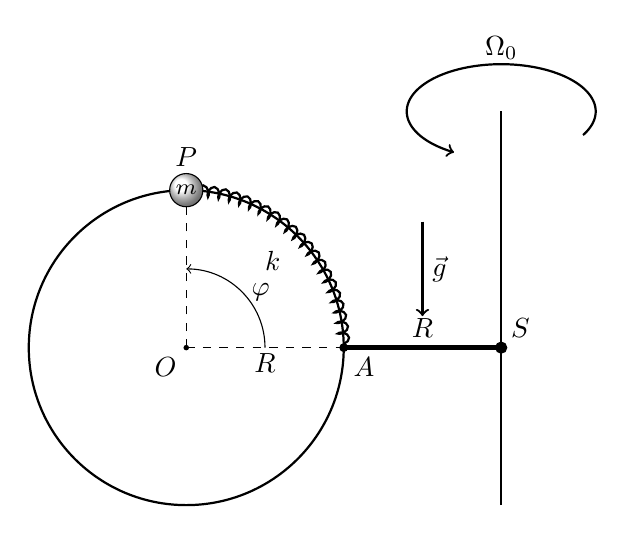
\begin{tikzpicture}[scale=2]
  % Radius
  \def\R{1}

  \coordinate (O) at (0,0);
  \coordinate (A) at (0,\R);
  \coordinate (P) at (\R,0);

  % Circle
  \draw[thick] (0,0) circle(\R);

  % Axes / radius lines
  \draw[dashed] (0,0) -- (0,\R);          % OA
  \draw[dashed] (0,0) -- (\R,0);          % OP

  % Points
  \fill (0,0) circle (0.5pt) node[below left] {$O$};
  \fill (0,\R) circle (1pt) node[above=5pt] {$P$};
 
  \fill (\R,0) circle (0.8pt) node[below right] {$A$};
  
        \draw[->] (0.5, 0) arc (0:90:0.5) node[midway, right] {$\varphi$};

  % Radius label
  \node at (0.5,-0.1) {$R$};
  \node[above] at (1.5*\R,0) {$R$};
  \filldraw (2*\R,0) circle (1pt) node[above right] {$S$};

  % Spring along arc from A to P (quarter circle, clockwise)
  \draw[decoration={coil, aspect=0.5, segment length=4pt, amplitude=2pt},
        decorate, thick] 
        (0,\R) arc[start angle=90, end angle=0, radius=\R];

  % Label for spring constant
  \node at (0.55,0.55) {$k$};

  
 \shadedraw[ball color=white] (0, \R) circle (3pt) node[font=\footnotesize] {$m$};
  % Horizontal bar from P to O (thick)
  \draw[line width=2pt] (\R,0) -- (2*\R,0);

  % Gravity vector
  \draw[->, thick] (1.5*\R,0.8) -- ++(0,-0.6);
  \node[right] at (1.5*\R,0.5) {$\vec{g}$};


 \draw[-,thick] (2,-1)--(2,1.5); 
    \begin{scope}[shift={(2,1.5)}, rotate=0]
    \draw[->,thick] 
      plot[domain=-30:240,variable=\t,smooth,samples=100] 
      ({0.6*cos(\t)}, {0.3*sin(\t)});
    \node at (0,0.4) {$\Omega_0$};
  \end{scope}

\end{tikzpicture}
    \caption{Sistema de anillo sobre aro circular giratorio con vínculo elástico.}
    \label{fig:anillo_aro}
\end{figure}

% --- SOLUCIÓN ---------------------------------------------------------------
\begin{solucion}{Anillo en aro circular con resorte}

\textbf{Marcos de referencia y Sistemas de Coordenadas}
\begin{itemize}
    \item $\mathcal{N}$: suelo (inercial) $\longrightarrow\{\vec{e}_x;\vec{e}_y;\vec{e}_z\}$, con origen en $S$ (punto del eje de giro a la altura de $O$).
    \item $\mathcal{A}$: aro $\longrightarrow\{\vec{e}_r;\vec{e}_\theta;\vec{e}_z\}$ (cilíndrica fija en el aro, con $\vec{e}_r$ horizontal desde el eje hacia el centro del aro).
    \item $\mathcal{B}$: marco imaginario orientado desde $O$ (centro del aro) hacia el anillo $P$ $\longrightarrow\{\vec{E}_r;\vec{E}_\varphi;\vec{e}_\theta\}$ en el plano del aro.
\end{itemize}

\begin{center}
\begin{tikzpicture}[>=Latex, scale=1.3]
    % --- PARÁMETROS ---
    \def\R{1.6}     % radio del aro [u]
    \def\ph{50}     % ángulo varphi [°]

    % --- EJE Y BARRA ---
    \draw[thick] (0,-1.5*\R) -- (0,1.7*\R);
    \draw[->, thick] (0,1.5*\R) -- (0,1.7*\R) node[above] {$\Omega_0$};
    \draw[line width=2pt] (0,0) -- (\R,0);
    \filldraw (0,0) circle (1.2pt) node[below left] {$S$};

    % --- ARO ---
    \coordinate (C) at (2*\R,0);
    \coordinate (A) at (\R,0);
    \coordinate (M) at ({2*\R-\R*cos(\ph)},{\R*sin(\ph)});
    \draw[thick] (C) circle (\R);
    \draw[dashed, gray] (C) -- (A);
    \draw[decoration={coil, aspect=0.5, segment length=3pt, amplitude=1.6pt}, decorate, thick]
        (A) arc (180:{180-\ph}:\R);
    \filldraw (C) circle (1pt) node[below right] {$O$};
    \filldraw (A) circle (1.2pt) node[below left] {$A$};
    \shadedraw[ball color=gray!30] (M) circle (3.5pt) node[above left] {$P$};

    % --- BASES ---
    \draw[azul, ultra thick, -{Latex}] (C) -- ++(0.9,0) node[right] {$\vec{e}_r$};
    \draw[azul, ultra thick, -{Latex}] (C) -- ++(0,0.9) node[right] {$\vec{e}_z$};
    \draw[myred, ultra thick, -{Latex}] (C) -- ({2*\R-0.9*cos(\ph)},{0.9*sin(\ph)}) node[below left, xshift=1pt, yshift=2pt] {$\vec{E}_r$};
    \draw[myred, ultra thick, -{Latex}] (M) -- ++({90-\ph}:0.9) node[above right] {$\vec{E}_\varphi$};
    \draw[->] ($(C)+(180:0.5)$) arc (180:{180-\ph}:0.5);
    \node at ({2*\R-0.75*cos(\ph/2)},{0.75*sin(\ph/2)-0.05}) {$\varphi$};
\end{tikzpicture}
\end{center}

\begin{equation*}
\begin{split}
    \vec{e}_r&=\cos(\Omega_0 t)\vec{e}_x+\sin(\Omega_0 t)\vec{e}_y\\
    \vec{e}_\theta&=-\sin(\Omega_0 t)\vec{e}_x+\cos(\Omega_0 t)\vec{e}_y\\
    \vec{E}_r&=-\cos\varphi\,\vec{e}_r+\sin\varphi\,\vec{e}_z\\
    \vec{E}_\varphi&=\sin\varphi\,\vec{e}_r+\cos\varphi\,\vec{e}_z
\end{split}
\end{equation*}

\textbf{Velocidad angular del aro}\\
$$\velang{N}{A}=\Omega_0\vec{e}_z\qquad\accang{N}{A}=\vec{0}$$

\subsubsection*{Cinemática de la partícula}
\textbf{Posición}\\
Como siempre, para obtener la velocidad respecto a un marco inercial partimos de la posición del anillo, medida desde un punto que no se mueve ($S$):
\begin{align*}
    \vec{r}_P &= 2R\,\vec{e}_r + R\,\vec{E}_r \\
              &= 2R\,\vec{e}_r + R\left[ -\cos\varphi\,\vec{e}_r + \sin\varphi\,\vec{e}_z \right] \\
              &= R\left(2 - \cos\varphi\right)\vec{e}_r + R\sin\varphi\,\vec{e}_z
\end{align*}

\textbf{Velocidad}\\
La velocidad es la derivada temporal de la posición:
\begin{align*}
\der{\vec{r}_P}{N}{} &= R \sin\varphi\,\dot{\varphi}\,\vec{e}_r + R(2 - \cos\varphi)\der{\vec{e}_r}{N}{} + R \cos\varphi\,\dot{\varphi}\,\vec{e}_z
\end{align*}

\patotruco{Aquí no hace falta escribir el teorema del transporte completo: como $\vec{e}_r$ y $\vec{e}_\theta$ solo giran en torno a $\vec{e}_z$ con velocidad angular $\Omega_0$, el trucazo es derivar $\vec{e}_r\to\Omega_0\vec{e}_\theta$ y $\vec{e}_\theta\to-\Omega_0\vec{e}_r$ (la demostración está en la Ayudantía 5).}

Derivadas temporales de $\vec{e}_r$ y $\vec{e}_\theta$:
$$\transport{\vec{e}_r}{N}{A}=\Omega_0\vec{e}_z\times\vec{e}_r=\Omega_0\vec{e}_\theta$$
$$\transport{\vec{e}_\theta}{N}{A}=\Omega_0\vec{e}_z\times\vec{e}_\theta=-\Omega_0\vec{e}_r$$
y finalmente
$$\marc{\vec{v}_P}{N}= R \sin\varphi\,\dot{\varphi}\,\vec{e}_r + R(2 - \cos\varphi)\,\Omega_0\,\vec{e}_\theta + R \cos\varphi\,\dot{\varphi}\,\vec{e}_z$$

\textbf{Aceleración}\\
Al igual que antes, derivamos la velocidad:
\begin{align*}
\marc{\vec{a}_P}{N}=\der{\vec{v}_P}{N}{} &= R \left[
\left( \ddot{\varphi} \sin\varphi + \dot{\varphi}^2 \cos\varphi - (2 - \cos\varphi) \Omega_0^2 \right) \vec{e}_r \right. \\
&\quad + \left(2 \dot{\varphi} \sin\varphi\, \Omega_0 \right) \vec{e}_\theta \\
&\quad + \left. \left( \ddot{\varphi} \cos\varphi - \dot{\varphi}^2 \sin\varphi \right) \vec{e}_z \right]
\end{align*}

\subsubsection*{Cinética}
\textbf{Diagrama de cuerpo libre}\\
Siempre se parte por un DCL, vista del plano $\vec{e}_r$-$\vec{e}_z$ (la normal $\vec{N}_\theta$ sale del plano):
\begin{center}
\begin{tikzpicture}[>=Latex, scale=1.0]
    \def\ph{50}
    \coordinate (M) at (0,0);
    \draw[->, thick, myred] (M) -- ++({180-\ph}:1.3) node[above left] {$\vec{N}_r$};
    \draw[->, thick, myred] (M) -- ++({270-\ph}:1.1) node[below left] {$\vec{F}_s$};
    \draw[->, thick, myred] (M) -- ++(0,-1.2) node[below] {$\vec{F}_g$};
    \shadedraw[ball color=gray!30] (M) circle (4pt);
    \node[above right] at (M) {$m$};
    \node at (1.3,0.9) {$\vec{N}_\theta$};
    \draw (1.8,0.9) circle (0.12); \fill (1.8,0.9) circle (1pt);
\end{tikzpicture}
\end{center}

Después del DCL se caracteriza cada fuerza vectorialmente. La fuerza de un resorte curvo tiene la dirección tangente de la curva en la que está contenido, en este caso $\vec{E}_\varphi$:
$$\vec{F}_s=-k(\ell-\ell_0)\vec{e}_t=-k(R\varphi-\ell_0)\vec{E}_{\varphi}=-k(R\varphi-\ell_0)\left(\sin\varphi\,\vec{e}_r+\cos\varphi\,\vec{e}_z\right)$$
$$\vec{F}_g=-mg\,\vec{e}_z$$
Al igual que en otros problemas, las direcciones de las normales son las direcciones normal y binormal de la curva:
$$\vec{N}_r=N_r\vec{E}_r=N_r\left( -\cos\varphi\,\vec{e}_r + \sin\varphi\,\vec{e}_z \right)$$
$$\vec{N}_\theta=N_\theta\vec{e}_\theta$$

\patoojo{El resorte curvo no tira en línea recta hacia $A$: su fuerza es tangente al aro y su largo es el arco $\ell=R\varphi$ (no la cuerda).}

\textbf{Ecuación diferencial}\\
Se plantea la segunda ley de Newton $\sum\vec{F}_{ext}=m\marc{\vec{a}_P}{N}$, proyectada en $\vec{e}_r$, $\vec{e}_\theta$ y $\vec{e}_z$:
\begin{align*}
-k(R\varphi-\ell_0)\sin\varphi - N_r\cos\varphi &= Rm \left( \ddot{\varphi} \sin\varphi + \dot{\varphi}^2 \cos\varphi - (2 - \cos\varphi) \Omega_0^2 \right)\\
N_\theta &= Rm \cdot 2 \dot{\varphi} \sin\varphi\, \Omega_0 \\
N_r\sin\varphi - mg - k(R\varphi - \ell_0)\cos\varphi &= Rm \left( \ddot{\varphi} \cos\varphi - \dot{\varphi}^2 \sin\varphi \right)
\end{align*}
Ignoramos la segunda ecuación, ya que no contiene $\ddot{\varphi}$.

\textbf{Paso 1: despejar $N_r$ de la primera ecuación.}
$$N_r = \frac{ -Rm \left( \ddot{\varphi} \sin\varphi + \dot{\varphi}^2 \cos\varphi - (2 - \cos\varphi) \Omega_0^2 \right) - k(R\varphi - \ell_0)\sin\varphi }{ \cos\varphi }$$

\textbf{Paso 2: sustituir $N_r$ en la tercera ecuación.}
\begin{multline*}
\left( \frac{ -Rm \left( \ddot{\varphi} \sin\varphi + \dot{\varphi}^2 \cos\varphi - (2 - \cos\varphi) \Omega_0^2 \right) - k(R\varphi - \ell_0)\sin\varphi }{ \cos\varphi } \right)\sin\varphi\\
- mg - k(R\varphi - \ell_0)\cos\varphi = Rm \left( \ddot{\varphi} \cos\varphi - \dot{\varphi}^2 \sin\varphi \right)
\end{multline*}

\textbf{Paso 3: expandir el lado izquierdo.}
\begin{multline*}
\frac{ -Rm \ddot{\varphi} \sin^2\varphi - Rm \dot{\varphi}^2 \cos\varphi\sin\varphi + Rm(2 - \cos\varphi) \Omega_0^2 \sin\varphi - k(R\varphi - \ell_0)\sin^2\varphi }{\cos\varphi}\\
- mg - k(R\varphi - \ell_0)\cos\varphi = Rm \ddot{\varphi} \cos\varphi - Rm \dot{\varphi}^2 \sin\varphi
\end{multline*}

\textbf{Paso 4: agrupar los términos con $\ddot{\varphi}$.}
$$\ddot{\varphi} \left( -Rm \left( \frac{\sin^2\varphi}{\cos\varphi} + \cos\varphi \right) \right)
= -Rm \ddot{\varphi} \cdot \frac{ \sin^2\varphi + \cos^2\varphi }{ \cos\varphi }
= -Rm \ddot{\varphi} \cdot \frac{1}{\cos\varphi}$$

\textbf{Paso 5: despejar $\ddot{\varphi}$.}\\
Multiplicamos ambos lados por $-\cos\varphi$ y el resultado es:
\respuesta{$\displaystyle \ddot{\varphi} = \frac{k(R\varphi - \ell_0) + mg \cos\varphi - Rm(2 - \cos\varphi)\, \Omega_0^2 \sin\varphi}{Rm}$}

\end{solucion}

\subsubsection{Partícula en ranura de disco giratorio}

Una partícula de masa $m$ se desliza dentro de una ranura recta en un disco rígido sin masa. La ranura está llena de un fluido que genera fricción en el movimiento de la partícula, cuyo coeficiente de fricción es $\nu$. El disco gira en el plano vertical con velocidad angular constante $\Omega$ en torno a un eje que pasa por el punto $O$, como se muestra en la Figura \ref{fig:disco_ranura}. Además, la ranura es ortogonal al diámetro del disco que contiene el punto $O$. Unido a la partícula hay un resorte lineal con constante de resorte $K$ y largo natural $\ell_0$. 

Utilizando el análisis de mecánica racional, realice lo siguiente:

\begin{enumerate}
    \item Defina los marcos de referencia y sistemas de coordenadas (fijo y móvil).
    \item Determine el vector posición, velocidad y aceleración de la partícula respecto al suelo.
    \item Identifique todas las fuerzas que actúan sobre la partícula (incluyendo la fuerza de fricción viscosa $\vec{F}_v = -\nu \vec{v}_{rel}$).
    \item Determine la ecuación diferencial de movimiento de la partícula en términos de la variable $x$.
\end{enumerate}

\begin{figure}[!ht]
    \centering
    \begin{tikzpicture}[>=Latex, scale=1.8]
        % --- Parámetros ---
        \def\ang{40}      % Ángulo Omega*t
        \def\distA{2}   % Distancia 'a' desde O al centro de la ranura
        \def\xPos{0.4}    % Posición x de la partícula respecto al centro
        \def\Rdisk{2.0}   % Radio visual del disco

        % --- Coordenadas ---
        \coordinate (O) at (0,0);
        % Dirección del diámetro (a lo largo de 'a')
        \coordinate (M) at ({\distA*sin(\ang)}, {-\distA*cos(\ang)});
        
        
        % --- 2. Soporte en O ---
        \begin{scope}
            \clip (-0.8,0.4) rectangle (0.4,-0.4);
            \fill[pattern=north east lines] (-0.3,0.1) rectangle (0.3,0.3);
            \filldraw[color=gris1!60] (0.2,0.1) arc (0:-180:0.2)--cycle;
            \draw[] (0.2,0.1) arc (0:-180:0.2)--cycle;
            \draw (-0.3,0.1) -- (0.3,0.1);
            
        \end{scope}
        % --- 1. Disco ---
        \shadedraw[inner color=white, outer color=gris1!20, draw=black, thick] (M) circle (\Rdisk);
        \filldraw (O) circle (1.5pt) node[below left] {$O$};
        
        % --- 3. Líneas de referencia ---
        \draw[dashed, gris1!60] (O) -- (0,-2.2);
        \draw[thick] (O) -- (M) node[midway, above right] {$a$};
        
        % Ángulo Omega*t
        \draw[->, azul] (0,-0.6) arc (270:{270+\ang}:0.6);
        \node[azul] at (0.2, -0.8) {$\Omega t$};

        % --- 4. Ranura y Partícula ---
        % Rotamos para dibujar la ranura perpendicular a OM
        \begin{scope}[shift={(M)}, rotate={\ang}]
            % Ranura (rectángulo)
            \draw[thick, fill=white] (-1, -0.2) rectangle (1, 0.2);
            
            % Eje x
            \draw[|->, thin] (0, -0.4) -- (0.8, -0.4) node[right] {$x$};
            \draw[|-|, thin] (-1, -0.4) --(0, -0.4) node[midway, below right] {$\ell_0$};
            

            % Resorte (desde Q a P)
            \draw[decoration={coil, segment length=4pt, amplitude=3pt}, decorate] 
                (-1, 0) -- (\xPos, 0) node[midway, right] {$K$};
            \filldraw (-1,0) circle (1pt) node[below] {$Q$};
            
            % Partícula P
            \shadedraw[ball color=gris1!20] (\xPos, 0) circle (4pt) node[above right, xshift=2pt] {$P$};
            \node[font=\footnotesize] at (\xPos, 0) {$m$};

        \end{scope}

        % --- 5. Gravedad ---
        \draw[->, thick, myred] (3.5, -0.5) -- (3.5, -1.3) node[midway, right] {$\vec{g}$};

    \end{tikzpicture}
    \caption{Esquema de una partícula con fricción viscosa y resorte en un disco rotatorio.}
    \label{fig:disco_ranura}
\end{figure}
\subsubsection{Partícula en superficie de un cono}

Una partícula $P$ de masa $m$ se mueve sin roce sobre la superficie exterior de un cono de ángulo $\phi = \pi/4$. El sistema se encuentra en el espacio profundo (sin gravedad). La partícula comienza su movimiento a una distancia $r_0$ del vértice, con una velocidad inicial perpendicular al eje $\vec{e}_z$ y una velocidad angular $\dot{\theta}(t_0) = \omega_0$. Además de la fuerza normal, existe una fuerza de atracción central ejercida por el eje $\vec{e}_z$ sobre la partícula:
\[ \vec{f} = -\frac{B}{\rho^2} \vec{e}_\rho \]
donde $B$ es una constante conocida y $\rho$ es la coordenada radial cilíndrica. Considerando el origen en el vértice del cono, realice lo siguiente:

\begin{enumerate}
    \item Defina los marcos de referencia y sistemas de coordenadas (esféricas y cilíndricas) adecuados.
    \item Encuentre la velocidad angular $\dot{\theta}$ de $P$ en función de la coordenada esférica $r$.
    \item Determine si la fuerza $\vec{f}$ es o no conservativa.
    \item Escriba la energía mecánica total en términos de $\dot{r}$ y $r$.
    \item Analice si existen soluciones donde la coordenada $r$ esté acotada entre dos valores, $r_{min}$ y $r_{max}$.
\end{enumerate}

\begin{figure}[!ht]
    \centering
    \begin{tikzpicture}[>=Latex, scale=1.5]
        % --- Parámetros ---
        \def\Rbase{2}
        \def\Hcone{2}
        \def\ang{45} % pi/4

        % --- 1. Dibujo del Cono ---
        % Elipse de la base (atrás)
        \draw[dashed, gray] (\Rbase, 0) arc (0:180:{\Rbase} and 0.6);
        % Superficie lateral
        \draw[thick] (-\Rbase, 0) -- (0, \Hcone) -- (\Rbase, 0);
        % Elipse de la base (adelante)
        \draw[thick] (-\Rbase, 0) arc (180:360:{\Rbase} and 0.6);

        % --- 2. Ejes y Ángulo ---
        \draw[->, dashed] (0, \Hcone) -- (0, -0.5) node[below] {$\vec{e}_z$};
        \draw[dashed] (0, \Hcone) -- +(0.8, -0.8);
        \draw[thin] (0, \Hcone-0.4) arc (270:315:0.4);
        \node at (0.2, \Hcone-0.6) {$\frac{\pi}{4}$};

        % --- 3. Partícula y Vectores ---
        % Posición de la partícula P
        \coordinate (V) at (0, \Hcone); % Vértice
        \coordinate (P) at (1.2, {\Hcone - 1.2}); % Punto en la superficie
        
        \filldraw[shading=ball, ball color=black] (P) circle (2.5pt) node[right, xshift=3pt] {$P$};
        
        % Vector e_r (A lo largo del cono)
        \draw[->, thick] (P) -- +(135:-0.8) node[right] {$\vec{e}_r$};
        % Vector e_phi (Perpendicular a la superficie)
        \draw[->, thick] (P) -- +(45:0.8) node[right] {$\vec{e}_\phi$};
        
        % Líneas auxiliares para rho
        \draw[dashed, gray] (P) -- (0, {\Hcone - 1.2});
        \node[above] at (0.6, {\Hcone - 1.2}) {$\rho$};

    \end{tikzpicture}
    \caption{Partícula $P$ en movimiento sobre la superficie de un cono bajo una fuerza central atractiva.}
    \label{fig:cono_particula}
\end{figure}
\subsubsection{Masa y resorte en el borde de una piscina}

Considere un sistema compuesto por un resorte y una masa que se encuentran al borde de una piscina muy profunda, como se indica en la Figura \ref{fig:piscina}. El resorte es de largo natural $\ell_0$ y constante elástica $k$. A éste se fija una pared móvil de masa despreciable. El sistema se prepara de tal modo que la partícula puntual de masa $m$ se coloca junto a esta pared en su posición de compresión máxima, es decir en $x = -\ell_0$, y se suelta desde el reposo.

\begin{enumerate}
    \item ¿Cuál es la condición que asegura que la masa $m$ se moverá desde $x = -\ell_0$?
    \item Encuentre el valor máximo de $\mu_d$ que permita a la masa llegar al borde de la piscina ($x = 0$) con velocidad no nula. Entregue el valor de esta velocidad.
    \item Una vez que entra a la piscina ($x > 0$), la masa experimenta una fuerza de roce viscoso lineal de constante $\gamma$. Suponga que no hay fuerza de empuje. Determine el alcance máximo y su velocidad límite.
\end{enumerate}

\begin{figure}[htbp]
    \centering
    \begin{tikzpicture}[>=Latex, scale=1.5]
        % --- Parámetros ---
        \def\Lzero{1.8} % Longitud L0
        
        % --- 1. El Suelo y la Piscina ---
        % Suelo (izquierda)
        \fill[gray!20] (-2.5, -2) rectangle (0, 0);
        \draw[thick] (-2.5, 0) -- (0, 0);
        \draw[pattern=north east lines, pattern color=gray!50] (-2.5, -2) rectangle (0, 0);
        
        % Piscina (derecha)
        \fill[blue!5] (0, -2) rectangle (2.5, 0);
        \draw[blue!40] (0, 0) -- (2.5, 0);
        % Líneas de agua
        \foreach \y in {-0.3, -0.7, -1.1, -1.5} {
            \draw[blue!30, thin] ({0.2-0.1*rand}, \y) -- ({2.3+0.1*rand}, \y);
        }
        \node[blue] at (0.5, -1) {$\gamma$};

        % --- 2. Ejes de Coordenadas ---
        \draw[->, thick] (-2.5, 0) -- (2.5, 0) node[right] {$x$};
        \draw[->, thick] (0, 0) -- (0, 1.2) node[above] {$y$};

        % --- 3. El Mecanismo (Muelle y Masa) ---
        % Pared fija
        \fill[gray!60] (-2.5, 0) rectangle (-2.2, 0.5);
        \draw[thick] (-2.2, 0) -- (-2.2, 0.5);
        
        % Resorte
        \draw[decoration={aspect=0.3, segment length=3pt, amplitude=3pt, coil}, decorate] 
            (-2.2, 0.25) -- (-\Lzero+0.2, 0.25);
        
        % Masa P
        \shadedraw[ball color=gray!80] (-\Lzero+0.2, 0.25) circle (7pt);
        \filldraw (-\Lzero+0.2, 0.25) circle (1pt); % centro
        
        % Cota L0
        \draw[|<->|] (-2.2, 0.7) -- (0, 0.7) node[midway, fill=white] {$\ell_0$};

        % --- 4. Traectoria de caída ---
        \draw[dashed, ->, gray] (0,0.15) parabola (1.8, -2);

        % --- 5. Etiquetas de coeficientes ---
        \node at (-1, -0.3) {$\mu_e, \mu_d$};
        \draw[->, thick] (1.2, 0.8) -- (1.2, 0.3) node[right] {$\mathbf{g}$};

    \end{tikzpicture}
    \caption{Sistema masa-resorte en el borde de una piscina con rozamiento seco y viscoso.}
    \label{fig:piscina}
\end{figure}
\subsubsection{Aro deslizante en brazo giratorio}

Un aro de masa $m$ se desliza sin fricción a lo largo de un brazo rígido sin masa de longitud variable. El brazo está articulado en uno de sus extremos en el punto $O$, el cual se encuentra en un eje vertical que gira con una velocidad angular constante $\Omega$. Además, el aro está unido a un resorte lineal con constante de resorte $K$ y largo natural $r_0$ conectado al punto $O$. El brazo puede girar libremente en el plano vertical. Utilizando las coordenadas $r$ (distancia al origen) y $\theta$ (ángulo con la vertical), realice lo siguiente:

\begin{enumerate}
    \item Defina los marcos de referencia y sistemas de coordenadas adecuados.
    \item Determine las expresiones para la energía cinética y potencial del sistema.
    \item Utilizando el formalismo de Lagrange, determine el sistema de dos ecuaciones diferenciales de movimiento para las variables $r$ y $\theta$.
\end{enumerate}

\begin{figure}[!ht]
    \centering
    \begin{tikzpicture}[>=Latex, scale=1.5]
        % --- Parámetros ---
        \def\ang{35} % Ángulo theta
        \def\rPos{2.2} % Posición r del aro

        % --- 1. Eje de Rotación ---
        \draw[dashed, thick] (0, 0.5) -- (0, -3.5);
        \draw[->, thick] (-0.3, 0.4) arc (180:450:0.3 and 0.1);
        \node[left] at (-0.3, 0.4) {$\Omega$};

        % Soporte O
        \fill[pattern=north east lines] (-0.3, 0) rectangle (0.3, 0.3);
        \draw[thick] (-0.3, 0) -- (0.3, 0);
        
        % --- 2. El Brazo y el Ángulo ---
        \begin{scope}[rotate=\ang]
            % El brazo
            \draw[line width=4pt, line cap=round] (0,0) -- (0, -3.2);
            \draw[line width=2.5pt, gray!60, line cap=round] (0,0) -- (0, -3.2);
            
            % El resorte
            \draw[decoration={aspect=0.3, segment length=3pt, amplitude=3.5pt, coil}, decorate] 
                (0,0) -- (0, -\rPos);
            \node[above right] at (0, -\rPos/2) {$K$};

            % El Aro (Masa m)
            \shadedraw[ball color=gray!30] (0, -\rPos) circle (0.1) node[font=\footnotesize] {$m$};
            
            % Cota r
            \draw[|<->|] (0.4, 0) -- (0.4, -\rPos) node[midway, above right] {$r$};
        \end{scope}

        % --- 3. Ángulo Theta ---
        \draw[dashed, gray] (0,0) -- (0, -1.5);
        \draw[->] (0, -0.8) arc (270:{270+\ang}:0.8);
        \node at (0.2, -1.0) {$\theta$};

        % --- 4. Articulación y Gravedad ---
        \filldraw[fill=gray!80] (0,0) circle (2pt) node[below left, xshift=-3pt] {$O$};
        \draw[->, thick] (1.7, -0.5) -- (1.7, -1.2) node[right] {$\mathbf{g}$};

    \end{tikzpicture}
    \caption{Sistema de un aro deslizante sobre un brazo rígido en rotación con vínculo elástico.}
    \label{fig:aro_brazo}
\end{figure}
% =========================================================================
% Capítulo 2: Cinética de la partícula
% Tema 01: Dinámica de la partícula
% Problema 09: Abrazadera en varilla horizontal con anclaje móvil
% Origen: Ayudantía 27, 2026
% =========================================================================
\subsubsection{Abrazadera en varilla horizontal con anclaje móvil}

Una abrazadera $P$ de masa $m$ desliza sin roce a lo largo de una varilla rígida, horizontal y fija (Figura \ref{fig:abrazadera}). Está unida a un resorte lineal de constante $k$ y largo natural $l_0$, cuyo otro extremo $Q$ se mueve con una ley prescrita $q(t)$. Tanto $q$ como la posición $x$ de la abrazadera se miden desde la pared izquierda, y $P$ se mantiene a la derecha de $Q$. No hay gravedad.

Resuelva usando trabajo y energía:
\begin{enumerate}
    \item Trate la fuerza del resorte como una fuerza externa (no conservativa) y obtenga la ecuación diferencial de $x(t)$ con el teorema de trabajo y energía.
    \item Trate el resorte como conservativo, con energía potencial $V(x,t)$. Calcule $dE/dt$ para $E=T+V$ y obtenga nuevamente la ecuación diferencial.
    \item Determine la potencia que debe entregar el mecanismo que mueve $Q$ y compárela con $dE/dt$.
\end{enumerate}

\begin{figure}[!ht]
    \centering
    \begin{tikzpicture}[>=Latex, scale=1.2]
        % --- PARÁMETROS ---
        \def\Lv{6.0}      % largo de la varilla [u]
        \def\xQ{1.9}      % posición del anclaje: q [u]
        \def\xP{4.5}      % posición de la abrazadera: x [u]

        % --- VARILLA Y PAREDES ---
        \draw[line width=4pt, gray!35] (0,0) -- (\Lv,0);
        \fill[pattern=north east lines] (-0.2,-0.45) rectangle (0,0.45);
        \draw[thick] (0,-0.45) -- (0,0.45);
        \draw[thick] (\Lv,-0.45) -- (\Lv,0.45);
        \fill[pattern=north east lines] (\Lv,-0.45) rectangle ({\Lv+0.2},0.45);

        % --- RESORTE, ANCLAJE Q Y ABRAZADERA P ---
        \draw[decorate, decoration={coil, aspect=0.4, segment length=3pt, amplitude=3pt}, thick] (\xQ,0) -- (\xP,0);
        \shadedraw[ball color=white!90] (\xQ,0) circle (0.13);
        \shadedraw[ball color=gray!30] (\xP,0) circle (0.13);
        \node[below=5pt] at (\xQ,0) {$Q$};
        \node[below=5pt] at (\xP,0) {$P$};
        \node[above=4pt] at ({(\xQ+\xP)/2},0) {$k$};
        \node[above=3pt, font=\small] at (\xP,0.02) {$m$};

        % --- COTAS ---
        \draw[|->, thick, gray] (0,0.75) -- (\xQ,0.75) node[midway, above] {$q(t)$};
        \draw[|-|, thick, gray] (\xQ,0.75) -- (\xP,0.75) node[midway, above] {$x-q$};
        \draw[|->, thick, gray] (0,-0.85) -- (\xP,-0.85) node[midway, below] {$x$};
        \draw[thin, gray] (\xQ,0.45) -- (\xQ,0.9);
        \draw[thin, gray] (\xP,-0.5) -- (\xP,-1.0);
    \end{tikzpicture}
    \caption{Abrazadera $P$ con anclaje móvil $Q$ y resorte lineal.}
    \label{fig:abrazadera}
\end{figure}

% --- SOLUCIÓN ---------------------------------------------------------------
\begin{solucion}{Abrazadera en varilla horizontal con anclaje móvil}

\textbf{Marcos de referencia y Sistemas de Coordenadas}\\
Basta un marco inercial fijo a la varilla, con $\vec{e}_x$ a lo largo de ella y origen en la pared izquierda.

\subsubsection*{Cinemática de la partícula}
Como $\vec{e}_x$ es constante, las posiciones se derivan directamente:
$$\vec{r}_P=x\vec{e}_x\qquad\vec{r}_Q=q\vec{e}_x\qquad\vec{v}_P=\dot{x}\vec{e}_x\qquad\vec{a}_P=\ddot{x}\vec{e}_x$$
El largo del resorte es $x-q$, su elongación es $\delta=x-q-l_0$ y su rapidez de deformación es $\dot\delta=\dot{x}-\dot{q}$. La abrazadera solo se traslada, sin rotar, así que
$$T=\frac{1}{2}m\dot{x}^2$$

\subsubsection*{Cinética}
Sobre la abrazadera actúan el resorte y la reacción de la varilla. La reacción es perpendicular a $\vec{e}_x$, o sea a la velocidad, y no trabaja: la única fuerza que trabaja es la del resorte.

\textbf{Diagrama de cuerpo libre}
\begin{center}
    \begin{tikzpicture}[>=Latex, scale=1.2]
        \draw[line width=4pt, gray!35] (-1.5,0) -- (2.5,0);
        \shadedraw[ball color=gray!30] (0,0) circle (0.14);
        \draw[->, thick, myred] (0,0) -- (-1.2,0) node[midway, above] {$k\delta$};
        \draw[->, thick, myred] (0,0) -- (0,0.9) node[above] {$N$};
        \draw[->, thick, azul] (0,-0.3) -- (1.2,-0.3) node[midway, below] {$\dot{x}$};
    \end{tikzpicture}
\end{center}
La fuerza del resorte sobre $P$ vale $\vec{F}_s=-k\delta\,\vec{e}_x$ (en la figura, con $\delta>0$, tira hacia $Q$).

\textbf{1) Resorte como fuerza no conservativa}\\
La energía cinética cambia solo por la potencia que entrega el resorte:
$$\frac{dT}{dt}=\vec{F}_s\cdot\vec{v}_P\quad\Longrightarrow\quad m\dot{x}\ddot{x}=-k\left(x-q-l_0\right)\dot{x}$$
Simplificando $\dot{x}$ (distinto de cero mientras la abrazadera se mueve):
\respuesta{$\displaystyle m\ddot{x}+k\left(x-q-l_0\right)=0$}

\textbf{2) Resorte como fuerza conservativa}\\
Incluimos el resorte en el potencial. Como el anclaje se mueve, $V$ depende explícitamente del tiempo:
$$V(x,t)=\frac{1}{2}k\left(x-q(t)-l_0\right)^2$$
Entonces $E=T+V$ no se conserva: su variación es la derivada parcial del potencial respecto al tiempo,
$$\frac{dE}{dt}=\frac{\partial V}{\partial t}=-k\left(x-q-l_0\right)\dot{q}$$
Desarrollando el lado izquierdo,
$$m\dot{x}\ddot{x}+k\left(x-q-l_0\right)\left(\dot{x}-\dot{q}\right)=-k\left(x-q-l_0\right)\dot{q}$$
los términos con $\dot{q}$ se cancelan y queda $m\dot{x}\ddot{x}+k\left(x-q-l_0\right)\dot{x}=0$. Al simplificar $\dot{x}$ resulta la misma ecuación:
\respuesta{$\displaystyle m\ddot{x}+k\left(x-q-l_0\right)=0\quad\text{es decir}\quad m\ddot{x}+kx=k\left(q(t)+l_0\right)$}
Es un oscilador de frecuencia natural $\omega_n=\sqrt{k/m}$ forzado por el anclaje. En la variable $\delta$ queda $\ddot\delta+\omega_n^2\delta=-\ddot{q}$: lo que excita al resorte es la \emph{aceleración} de $Q$.

% NOTA PARA REVISIÓN (agente B): el ítem 3 (potencia del mecanismo) NO está resuelto en Ay27S.tex;
% el desarrollo de abajo es una derivación propia del agente, consistente con el dE/dt de arriba.
\textbf{3) Potencia del mecanismo que mueve $Q$}\\
El resorte tira de $Q$ con $+k\delta\,\vec{e}_x$ (hacia $P$), de modo que el mecanismo debe ejercer $-k\delta\,\vec{e}_x$ para imponer $q(t)$. Su potencia es
$$\mathcal{P}_{mec}=\left(-k\delta\,\vec{e}_x\right)\cdot\dot{q}\,\vec{e}_x=-k\left(x-q-l_0\right)\dot{q}$$
que coincide con $dE/dt=\partial V/\partial t$: la energía de $E=T+V$ varía solo por lo que entrega (o absorbe) el mecanismo que mueve $Q$.

\end{solucion}

\subsubsection{Partícula en resorte con anclaje móvil}

Una partícula de masa $m$ está unida a un resorte lineal con constante elástica $k$ y longitud natural $r_0$ El otro extremo del resorte está conectado a una abrazadera sin masa que se desliza sobre una guía horizontal sin fricción, cuyo desplazamiento $x(t)$ respecto a un origen fijo es conocido. Sabiendo que la gravedad actúa hacia abajo, se requiere analizar el comportamiento dinámico del sistema mostrado en la Figura \ref{fig:particula_resorte_movil}.

\begin{enumerate}
    \item Defina los marcos de referencia y sistemas de coordenadas adecuados.
    \item Determine y analice la cinemática de la partícula utilizando las variables $r$ y $\theta$.
    \item Determine y analice la cinética de la partícula para obtener las ecuaciones diferenciales de movimiento.
\end{enumerate}

\begin{figure}[!ht]
    \centering
    \begin{tikzpicture}[>=Latex, scale=1.5]
        % --- Parámetros de diseño ---
        \def\rL{3.0}      % Longitud del dibujo para r
        \def\ang{35}     % Ángulo theta
        \def\guideW{3.5}  % Ancho de la guía
        
        % --- Coordenadas ---
        \coordinate (Origin) at (-2, 0);       % Referencia fija
        \coordinate (O) at (0.5, 0);           % Posición de la abrazadera
        \coordinate (P) at ($(O) + ({\rL*sin(\ang)}, {-\rL*cos(\ang)})$); % Partícula
        
        % --- 1. Guía horizontal y soportes ---
        \draw[line width=3pt, black] (-\guideW, 0) -- (\guideW, 0);
        \draw[line width=2.5pt, gris1!40] (-\guideW, 0) -- (\guideW, 0);
        % Soporte Izquierdo
        \fill[pattern=north east lines] (-\guideW-0.3, -0.4) rectangle (-\guideW, 0.4);
        \draw[thick] (-\guideW, -0.4) -- (-\guideW, 0.4);
        % Soporte Derecho
        \fill[pattern=north east lines] (\guideW, -0.4) rectangle (\guideW+0.3, 0.4);
        \draw[thick] (\guideW, -0.4) -- (\guideW, 0.4);

        % --- 2. Abrazadera O ---
        \shadedraw[ball color=gris1!10, draw=black] (O) ellipse (0.15 and 0.15);
        \node[below left, xshift=-2pt] at (O) {$O$};
        \draw[black] (O) circle (0.15);

        % --- 3. Desplazamiento x(t) ---
        \draw[dashed, thin] (Origin) -- (Origin);
        \draw[dashed, thin] (Origin) -- ++(0, 0.8);
        \draw[dashed, thin] (O) -- ++(0, 0.8);
        \draw[|->, thick] ($(Origin)+(0,0.6)$) -- ($(O)+(0,0.6)$) node[midway, above] {$x(t)$};

        % --- 4. Resorte y Coordenadas ---
        % Línea de referencia vertical
        \draw[dashed, gris1!60] (O) -- ++(0, -3.5);
        
        % Resorte
        \draw[decoration={aspect=0.4, segment length=3mm, amplitude=3mm, coil}, decorate, thick] (O) -- (P);
        \node[left, xshift=-8pt] at ($(O)!0.5!(P)$) {$k$};

        % Ángulo theta
        \draw[->] (0.5, -0.8) arc (270:{270+\ang}:0.8);
        \node at (0.7, -1.0) {$\theta$};

        % Vector r (distancia)
        \draw[|<->|, thin] ($(O)+(0.4, 0.2)$) -- ($(P)+(0.4, 0.2)$) node[midway, above right] {$r$};

        % --- 5. Partícula P ---
        \shadedraw[ball color=gris1!30] (P) circle (0.2);
        \node at (P) {$m$};
        \node[right, xshift=10pt] at (P) {$P$};

        % --- 6. Vector de gravedad ---
        \draw[->, thick, myred] (-2.5, -1.5) -- (-2.5, -2.5) node[midway, left] {$\mathbf{g}$};

    \end{tikzpicture}
    \caption{Esquema de una partícula $m$ acoplada a un resorte con soporte móvil $x(t)$.}
    \label{fig:particula_resorte_movil}
\end{figure}

% =========================================================================
% Capítulo 2: Cinética de la partícula
% Tema 01: Dinámica de la partícula
% Problema 11: Collar en riel circular con resorte excéntrico
% Origen: Ayudantía 27, 2026
% =========================================================================
\subsubsection{Collar en riel circular con resorte excéntrico}

Un collar de masa $m$ desliza sin roce sobre un riel circular de radio $R$ contenido en un plano horizontal, como se muestra en la Figura \ref{fig:collar_riel}. El collar está unido a un punto fijo $A$ mediante un resorte de constante elástica $K$ y largo natural nulo. El punto $A$ está a una distancia $2R$ del centro $O$ del riel, sobre la recta horizontal de referencia. La posición del collar se mide con el ángulo $\phi$ desde esa recta, en sentido antihorario. No hay gravedad, y las condiciones iniciales son $\phi_0$ y $\dot\phi_0$.

Resuelva usando trabajo y energía:
\begin{enumerate}
    \item Obtenga la ecuación diferencial del movimiento de $\phi(t)$.
    \item Determine $\dot\phi$ como función de $\phi$.
    \item Calcule la fuerza de reacción del riel sobre el collar en función de $\phi$.
    \item Encuentre las posiciones de equilibrio, determine su estabilidad y la frecuencia de las oscilaciones pequeñas alrededor de la estable.
\end{enumerate}

\begin{figure}[!ht]
    \centering
    \begin{tikzpicture}[>=Latex, scale=1.5]
        % --- Parámetros ---
        \def\R{1.5}          % Radio del riel
        \def\ang{30}         % Ángulo phi
        \def\distA{2*\R}     % Distancia OA

        % --- 1. Riel Circular ---
        \draw[thick] (0,0) circle (\R);
        \draw[dashed] (-\distA-0.5, 0) -- (\R+0.5, 0); % Eje horizontal de referencia
        \filldraw (0,0) circle (1.5pt) node[below] {$O$};

        % --- 2. Punto Fijo A ---
        \coordinate (A) at (-\distA, 0);
        \fill[pattern=north east lines] (-\distA-0.3, -0.2) rectangle (-\distA, 0.2);
        \draw[thick] (-\distA, -0.2) -- (-\distA, 0.2);
        \filldraw (A) circle (2pt) node[below right] {$A$};

        % --- 3. Posición del Collar ---
        \coordinate (M) at ({\R*cos(\ang)}, {\R*sin(\ang)});
        
        % Radio R y Ángulo phi
        \draw[dashed] (0,0) -- (M);
        \draw[->] (0.6, 0) arc (0:\ang:0.6);
        \node at (0.8, 0.2) {$\phi$};
        \node at (0.4, 0.4) {$R$};

        % --- 4. Resorte ---
        \draw[decoration={aspect=0.3, segment length=3pt, amplitude=2.5pt, coil}, decorate] 
            (A) -- (M);
        \node[above] at ($(A)!0.5!(M)$) {$K$};

        % --- 5. Masa m (Collar) ---
        \shadedraw[ball color=gray!30] (M) circle (0.15);
        \node[above right] at (M) {$m$};

        % --- 6. Vector de Gravedad (indicativo de plano horizontal) ---
        % Nota: El enunciado dice sin gravedad, pero se incluye el vector 
        % tachado o lateral para cumplir con la regla de formato visual.
        %\draw[->, thick] (2, 1) -- (2, 0.5) node[midway, right] {$\mathbf{g}$};

    \end{tikzpicture}
    \caption{Diagrama de un collar de masa $m$ deslizando en un riel circular con vínculo elástico desde un punto exterior.}
    \label{fig:collar_riel}
\end{figure}

% --- SOLUCIÓN ---------------------------------------------------------------
% NOTA PARA REVISIÓN (agente B): el ítem 4 (equilibrios, estabilidad y frecuencia de pequeñas
% oscilaciones) NO está resuelto en Ay27S.tex ni en Ay3S.tex; se mantiene en el enunciado sin solución.
\begin{solucion}{Collar en riel circular con resorte excéntrico}

\textbf{Marcos de referencia y Sistemas de Coordenadas}\\
Lo primero, como en todo ejercicio, es definir los marcos de referencia.
\begin{itemize}
    \item $\mathcal{N}$: el suelo $\longrightarrow\{\vec{e}_x;\vec{e}_y;\vec{e}_z\}$
    \item $\mathcal{A}$: cilíndrico $OM$ $\longrightarrow\{\vec{e}_r;\vec{e}_\theta;\vec{e}_z\}$
\end{itemize}

\begin{center}
\begin{tikzpicture}[scale=0.8]
    \Polaresrtz{\phi}{e}{e}{azul}{myred}
    \node[below right] at (35:2) {$m$};
\end{tikzpicture}
\end{center}

\begin{equation*}
\begin{split}
    \vec{e}_r&=\cos\phi\,\vec{e}_x+\sin\phi\,\vec{e}_y\\
    \vec{e}_\theta&=-\sin\phi\,\vec{e}_x+\cos\phi\,\vec{e}_y\\
    \vec{e}_z&=\vec{e}_z
\end{split}
\end{equation*}

\subsubsection*{Cinemática de la partícula}
\textbf{Posición}\\
Como siempre, para obtener la velocidad de algún punto respecto a un marco de referencia inercial partimos por la posición; en este caso la de la masa $m$ es
$$\vec{r}_m=R\,\vec{e}_r$$

\textbf{Velocidad}\\
La velocidad es la derivada temporal de la posición:
$$\marc{\vec{v}_m}{N}=\der{\vec{r}_{m}}{N}=\der{(R\vec{e}_r)}{N}=R\der{\vec{e}_r}{N}{}$$

\patotruco{No es necesario usar el teorema del transporte completo: usamos el trucazo (la demostración está en la Ayudantía 5). Basta con derivar la base: $\dot{\vec{e}}_r=\dot\phi\,\vec{e}_\theta$ y $\dot{\vec{e}}_\theta=-\dot\phi\,\vec{e}_r$.}

Derivadas temporales de $\vec{e}_r$ y $\vec{e}_\theta$:
$$\transport{\vec{e}_r}{N}{A}=\dot\phi\vec{e}_z\times\vec{e}_r=\dot\phi\vec{e}_\theta$$
$$\transport{\vec{e}_\theta}{N}{A}=\dot\phi\vec{e}_z\times\vec{e}_\theta=-\dot\phi\vec{e}_r$$
y finalmente
$$\marc{\vec{v}_m}{N}=R\dot\phi\,\vec{e}_\theta$$

\textbf{Aceleración}\\
Al igual que antes, podemos simplemente derivar la velocidad:
% NOTA PARA REVISIÓN (agente B): el zip escribe +R*phi'^2 e_r; el signo correcto es -R*phi'^2 e_r
% (y es el que se usa más abajo en Newton). Se deja tal cual.
$$\marc{\vec{a}_m}{N}=\der{\marc{\vec{v}_m}{N}{}}{N}{}=\der{\left(R\dot\phi\,\vec{e}_\theta\right)}{N}{}=(R\dot\phi^2)\vec{e}_r+ R\ddot\phi\,\vec{e}_{\theta}$$

\subsubsection*{Cinética}
\textbf{Diagrama de cuerpo libre}\\
Siempre se parte por un DCL:
\begin{center}
\begin{tikzpicture}[>=Latex, scale=1.1]
    \def\R{1.5}
    \def\ang{35}
    \draw[thick] (0,0) circle (\R);
    \coordinate (A) at ({-2*\R},0);
    \coordinate (M) at ({\R*cos(\ang)},{\R*sin(\ang)});
    \filldraw (A) circle (1.5pt) node[below] {$A$};
    \filldraw (0,0) circle (1pt) node[below] {$O$};
    \draw[dashed, gray] (A) -- (M);
    \draw[->, very thick, orange!80!black] (M) -- ($(M)!0.45!(A)$) node[below, pos=0.9] {$\vec{F}_s$};
    \draw[->, very thick, violet!80!black] (M) -- ++(\ang:0.9) node[above right] {$\vec{N}$};
    \shadedraw[ball color=gray!30] (M) circle (4pt);
\end{tikzpicture}
\end{center}
Después del DCL se caracteriza cada fuerza vectorialmente:
$$\vec{F}_s=-K(\ell-\ell_0)\vec{u}_s;\quad \ell=\|R\vec{e}_r+2R\vec{e}_x\|;\quad\ell_0=0;\quad\vec{r}-\vec{r}_A=(R\vec{e}_r)-(-2R\vec{e}_x)$$
$$\vec{u}_s = \frac{\vec{r} - \vec{r}_A}{\left\lVert \vec{r} - \vec{r}_A \right\rVert}=\frac{R\vec{e}_r+2R\vec{e}_x}{\|R\vec{e}_r+2R\vec{e}_x\|}$$
$$\vec{F}_s=-K\|R\vec{e}_r+2R\vec{e}_x\|\frac{\vec{r} - \vec{r}_A}{\left\lVert \vec{r} - \vec{r}_A \right\rVert}=-K(R\vec{e}_r+2R\vec{e}_x)$$
En este caso tenemos dos normales, pero como el problema es 2D una de ellas desaparece, y la dirección se obtiene mediante intuición o matemáticamente con las coordenadas intrínsecas de la curva, en este caso un círculo:
$$\vec{N}=N\vec{e}_r$$

\textbf{Energía}\\
Si lo hacemos con energía tenemos
$$T=\frac{1}{2}m\left|\vec{v}_P\right|^2=\frac{1}{2}mR^2\dot\phi^2$$
El punto $A$ está fijo en $\vec{r}_A=-2R\,\vec{e}_x$. El vector que va de $A$ al collar es $R\vec{e}_r+2R\vec{e}_x$, y como $\vec{e}_x=\cos\phi\,\vec{e}_r-\sin\phi\,\vec{e}_\theta$,
$$\vec{r}_P-\vec{r}_A=R\left(1+2\cos\phi\right)\vec{e}_r-2R\sin\phi\,\vec{e}_\theta$$
$$\ell^2=R^2\left[\left(1+2\cos\phi\right)^2+4\sin^2\phi\right]=R^2\left(5+4\cos\phi\right)$$
Como el largo natural es nulo, la elongación es el propio $\ell$ y
$$V=\frac{1}{2}K\ell^2=\frac{1}{2}KR^2\left(5+4\cos\phi\right)$$
La conservación de la energía mecánica, con $\phi_0$ y $\dot\phi_0$ como condiciones iniciales, es
$$\frac{1}{2}mR^2\dot\phi^2+\frac{1}{2}KR^2\left(5+4\cos\phi\right)=\frac{1}{2}mR^2\dot\phi_0^2+\frac{1}{2}KR^2\left(5+4\cos\phi_0\right)$$
Derivando respecto al tiempo, $mR^2\dot\phi\ddot\phi-2KR^2\sin\phi\,\dot\phi=0$, y simplificando $mR^2\dot\phi$:
\respuesta{$\displaystyle \ddot\phi=\frac{2K}{m}\sin\phi$}

\textbf{Segunda ley de Newton}
$$\sum \vec{F} = m \vec{a}$$
$$\sum \vec{F} = \vec{N} + \vec{F}_s = \left[ N - KR(1 + 2\cos\phi) \right] \vec{e}_r + 2KR \sin\phi \, \vec{e}_\theta$$
$$\sum F_{\vec{e}_r} = N - KR(1 + 2\cos\phi) = m(-R\dot{\phi}^2)$$
$$\sum F_{\vec{e}_\theta} = 2KR \sin\phi = m(R\ddot{\phi})\quad\Longrightarrow\quad\ddot{\phi} - \frac{2K}{m} \sin\phi = 0$$
que coincide con lo obtenido por energía. De la ecuación en $\vec{e}_r$:
$$N = -mR\dot{\phi}^2 + KR(1 + 2\cos\phi)$$

\textbf{Fuerza de reacción en función de $\phi$}\\
Queremos la expresión en función de $\phi$, no de $\dot{\phi}$. De la segunda EDO tenemos $\ddot{\phi} = \frac{2K}{m} \sin\phi$. Usamos el truco
$$\ddot{\phi} = \frac{d\dot{\phi}}{dt} = \frac{d\dot{\phi}}{d\phi} \cdot \frac{d\phi}{dt} = \dot{\phi} \frac{d\dot{\phi}}{d\phi}$$
(que deja el diferencial en función de $\phi$). Sustituimos e integramos ambos lados:
$$\dot{\phi} \frac{d\dot{\phi}}{d\phi} = \frac{2K}{m} \sin\phi\quad\Longrightarrow\quad\int_{\dot{\phi}_0}^{\dot{\phi}} \dot{\phi} \, d\dot{\phi} = \int_{\phi_0}^{\phi} \frac{2K}{m} \sin\phi \, d\phi$$
$$\frac{\dot{\phi}^2}{2} - \frac{\dot{\phi}_0^2}{2} = -\frac{2K}{m} (\cos\phi - \cos\phi_0)$$
y reordenando:
\respuesta{$\displaystyle \dot{\phi}^2 = \dot{\phi}_0^2 + \frac{4K}{m} (\cos\phi_0 - \cos\phi)$}
Reemplazando en la ecuación de $N$:
% NOTA PARA REVISIÓN (agente B): en el zip el resultado final conserva -mR*phi'^2 (debería ser -mR*phi'_0^2
% tras sustituir). Se deja tal cual.
\begin{align*}
N &= -mR\left[ \dot{\phi}^2_0 + \frac{4K}{m}(\cos \phi_0 - \cos \phi) \right] + KR(1 + 2\cos\phi) \\
  &= -mR\dot{\phi}^2 - 4KR(\cos \phi_0 - \cos \phi) + KR(1 + 2\cos\phi) \\
  &= -mR\dot{\phi}^2 - 4KR\cos \phi_0 + 6KR\cos \phi + KR
\end{align*}
Por lo tanto, la fuerza de reacción ejercida sobre la partícula es:
\respuesta{$\displaystyle \vec{N} = \left[ -mR\dot{\phi}^2 - 4KR\cos \phi_0 + 6KR\cos \phi + KR \right] \vec{e}_r$}

\end{solucion}

% =========================================================================
% Capítulo 2: Cinética de la partícula
% Tema 01: Dinámica de la partícula
% Problema 12: Partícula en pista parabólica rotatoria
% Origen: Ayudantía 3, 2026
% =========================================================================
\subsubsection{Partícula en pista parabólica rotatoria}

Una partícula de masa $m$ se desliza sin fricción a lo largo de una pista en forma de parábola como se muestra en la \text{Figura \ref{fig:parabola_rotatoria}}. La ecuación que describe la geometría de la pista está dada por:
\[ y = \frac{r^2}{2a} \]
donde $a$ es una constante, $r$ es la distancia radial desde el eje vertical de simetría (punto $O$ al punto $B$), y $y$ es la distancia vertical desde el origen $O$ al punto $Q$. 

La partícula está unida a un resorte lineal de constante elástica $k$ y longitud natural $\ell_0$. El resorte se mantiene siempre alineado horizontalmente, conectando la partícula con un punto de unión libre de deslizarse a lo largo del eje vertical que pasa por el centro de la parábola. El sistema completo rota con una velocidad angular constante $\Omega$ alrededor de la dirección vertical. Considerando que la gravedad $\mathbf{g}$ actúa verticalmente hacia abajo, realice lo siguiente:

\begin{enumerate}
    \item Defina los marcos de referencia y sistemas de coordenadas adecuados para describir el movimiento en términos de la variable $r$.
    \item Analice la cinemática de la partícula, determinando el momento lineal y el momento angular respecto al punto $Q$.
    \item Analice la cinética de la partícula y determine la ecuación diferencial del movimiento en términos de la variable $r$.
\end{enumerate}

\begin{figure}[!ht]
    \centering
\begin{tikzpicture}[scale=1.2]
  % Axes
  \draw[->] (-3,0) -- (3,0) node[right] {$x$};
  \draw[-] (0,0) -- (0,4) ;

  % Origin
  \node[below left] at (0,0) {$O$};

  % Parabola
  \draw[domain=-2.5:2.5,smooth,variable=\x,thick] 
    plot ({\x},{0.5*\x*\x});

  % Dashed guides to Q
  \node[below, right] at (2,-0.15) {$B$};
    \filldraw[black] (2,0) circle (1.5pt);
  \draw[dashed] (0,0) -- (0,2) node[left] {$Q$};
    \filldraw[black] (0,2) circle (1.5pt);

  % Spring from Q to m
  \draw[decorate,decoration={coil,aspect=0.3, segment length=3mm, amplitude=2pt}, thick]
    (0,2) --node[midway,above] {$k$} (2,2);

  % Mass at end of spring
  \filldraw[fill=gray!30,draw=black] (2,2) circle (2pt);
  \node[right] at (2,2) {$m$};

  % Vertical arrow from parabola to mass: y
  \draw[->,thick] (2,0) -- (2,1.9);
  \node[right] at (2,1.2) {$y$};

  % Gravity arrow g
  \draw[->,thick] (3,4) -- (3,3);
  \node[right] at (3,3.5) {$\mathbf{g}$};

  \begin{scope}[shift={(0,3.5)}, rotate=0]
    \draw[->,thick] 
      plot[domain=-30:240,variable=\t,smooth,samples=100] 
      ({0.6*cos(\t)}, {0.3*sin(\t)});
    \node at (-0.8,0.4) {$\Omega$};
  \end{scope}
    % Axis stub and triangle tip
  \draw[thick] (0,3.5) -- (0,4.2);
  \draw[fill=black] (0,4.2) -- (-2pt,3.9) -- (2pt,3.9) -- cycle;

  %FLECHA r
  

\draw[-,dashed] (0,0)--(0,-0.5);
\draw[-,thick] (0,-0.5) -- node[midway, above] {$r$} (2,-0.5);
\draw (0,-0.4) -- (0,-0.6);
\draw (2,-0.4) -- (2,-0.6);

\end{tikzpicture}
    \caption{Diagrama de una partícula de masa $m$ en una pista parabólica rotatoria con vínculo elástico horizontal.}
    \label{fig:parabola_rotatoria}
\end{figure}

% --- SOLUCIÓN ---------------------------------------------------------------
\begin{solucion}{Partícula en pista parabólica rotatoria}

\textbf{Marcos de referencia y Sistemas de Coordenadas}\\
Lo primero, como en todo ejercicio, es definir los marcos de referencia.
\begin{itemize}
    \item $\mathcal{N}$: el suelo $\longrightarrow\{\vec{e}_x;\vec{e}_y;\vec{e}_z\}$
    \item $\mathcal{A}$: parábola $\longrightarrow\{\vec{e}_r;\vec{e}_\theta;\vec{e}_z\}$
\end{itemize}

\begin{center}
\begin{tikzpicture}[scale=0.8]
    \Polaresrtz{\Omega t}{e}{e}{azul}{myred}
    \node[above right] at (35:2) {$P$};
\end{tikzpicture}
\end{center}

\begin{equation*}
\begin{split}
    \vec{e}_r&=\cos(\Omega t)\vec{e}_x+\sin(\Omega t)\vec{e}_y\\
    \vec{e}_\theta&=-\sin(\Omega t)\vec{e}_x+\cos(\Omega t)\vec{e}_y\\
    \vec{e}_z&=\vec{e}_z
\end{split}
\end{equation*}

\subsubsection*{Cinemática de la partícula}
\textbf{Posición}\\
Como siempre, para obtener la velocidad de algún punto respecto a un marco inercial partimos por la posición; en este caso la de la masa $m$ es
$$\vec{r}_m=r\vec{e}_r+y\vec{e}_z$$

\textbf{Velocidad}\\
La velocidad es la derivada temporal de la posición:
$$\marc{\vec{v}_m}{N}=\der{\vec{r}_{m}}{N}=\der{(r\vec{e}_r+ y\vec{e}_z)}{N}=\dot r\vec{e}_r+r\der{\vec{e}_r}{N}{}+\dot y\vec{e}_z$$

\patotruco{No es necesario usar el teorema del transporte completo: usamos el trucazo (la demostración está en la Ayudantía 5). Como $\vec{e}_r$ y $\vec{e}_\theta$ giran solo en torno a $\vec{e}_z$ con velocidad angular $\Omega$, basta con $\dot{\vec{e}}_r=\Omega\vec{e}_\theta$ y $\dot{\vec{e}}_\theta=-\Omega\vec{e}_r$.}

Derivadas temporales de $\vec{e}_r$ y $\vec{e}_\theta$:
$$\transport{\vec{e}_r}{N}{A}=\Omega\vec{e}_z\times\vec{e}_r=\Omega\vec{e}_\theta$$
$$\transport{\vec{e}_\theta}{N}{A}=\Omega\vec{e}_z\times\vec{e}_\theta=-\Omega\vec{e}_r$$
y finalmente
$$\marc{\vec{v}_m}{N}=\dot r\vec{e}_r+r\Omega\vec{e}_\theta+\dot y\vec{e}_z$$

\textbf{Aceleración}\\
Al igual que antes, podemos simplemente derivar la velocidad:
% NOTA PARA REVISIÓN (agente B): el zip escribe -2 r' Omega e_theta; derivando la velocidad
% de arriba el signo es +2 r' Omega e_theta. Se deja tal cual (y arrastra el signo a N_b).
$$\marc{\vec{a}_m}{N}=\der{\marc{\vec{v}_m}{N}{}}{N}{}=\der{\left(\dot r\vec{e}_r+r\Omega\vec{e}_\theta+\dot y\vec{e}_z\right)}{N}{}=(\ddot{r}-r\Omega^2)\vec{e}_r-2\dot r\Omega\vec{e}_{\theta}+\ddot{y}\vec{e}_z$$
Obteniendo las derivadas de $y$ podemos reemplazar:
$$\dot y=\dfrac{r\dot r}{a}\qquad\ddot y=\dfrac{\dot r^2+r\ddot r}{a}$$

\textbf{Momento lineal y angular}\\
Para el cálculo del momento lineal hay que recordar cómo se define, y en este caso es
% NOTA PARA REVISIÓN (agente B): el zip escribe \dot y e_y en el momento lineal; por el contexto es \dot y e_z.
$$\marc{}{N}\vec{G}=m\cdot \marc{\vec{v}}{N}=m(\dot r\vec{e}_r+r\Omega\vec{e}_\theta+\dot y\vec{e}_y)$$
Por otro lado, el momento angular se tiene que calcular respecto a un punto; por ejemplo, podemos obtenerlo respecto al punto $Q$:
$$\marc{}{N}\vec{H}_Q=(\vec{r}_m-\vec{r}_Q)\times m(\vec{v}_m-\vec{v}_Q)$$
$$\marc{}{N}\vec{H}_Q=(r\vec{e}_r)\times m(\dot r\vec{e}_r+r\Omega\vec{e}_\theta)=mr^2\Omega\vec{e}_z$$

\subsubsection*{Cinética}
\textbf{Diagrama de cuerpo libre}\\
Cuando se hace análisis cinético hay que contar todas las cosas que uno elimina del problema y reemplazarlas por una fuerza; en este caso, cuando nos quedamos solo con la partícula:

\begin{center}
\begin{tikzpicture}[>=Latex, scale=1.0]
    % --- PARÁMETROS ---
    \def\a{1.5}       % constante de la parábola [u]
    \def\rp{1.8}      % posición radial de la partícula [u]

    % --- EJE Y PARÁBOLA ---
    \draw[->, thin] (0,-0.2) -- (0,3.1) node[above] {$\vec{e}_z$};
    \draw[thick, domain=0:2.6, smooth, samples=40, variable=\x] plot ({\x},{\x*\x/(2*\a)});
    \draw[->, thin] (0,0) -- (3.0,0) node[right] {$\vec{e}_r$};

    % --- PARTÍCULA Y BASE TNB ---
    \pgfmathsetmacro{\yp}{\rp*\rp/(2*\a)}
    \pgfmathsetmacro{\nrm}{sqrt(1+(\rp/\a)^2)}
    \coordinate (M) at (\rp,\yp);
    \draw[dashed, gray] (M) -- (0,\yp);
    \draw[dashed, gray] (M) -- (\rp,0) node[below] {\textcolor{gray}{$r$}};
    \draw[->, ultra thick, myred] (M) -- ++({1/\nrm},{(\rp/\a)/\nrm}) node[right] {$\vec{e}_t$};
    \draw[->, ultra thick, azul] (M) -- ++({-(\rp/\a)/\nrm},{1/\nrm}) node[above] {$\vec{e}_n$};
    \draw (M) ++(0.3,-0.3) circle (0.1); \draw ($(M)+(0.3,-0.3)+(-0.07,-0.07)$) -- ++(0.14,0.14); \draw ($(M)+(0.3,-0.3)+(-0.07,0.07)$) -- ++(0.14,-0.14);
    \node[green!50!black, right] at ($(M)+(0.4,-0.3)$) {$\vec{e}_b=\vec{e}_\theta$};
    \shadedraw[ball color=gray!30] (M) circle (3pt);
\end{tikzpicture}
\hspace{1cm}
\begin{tikzpicture}[>=Latex, scale=1.0]
    \def\a{1.5}
    \def\rp{1.8}
    \draw[->, thin] (0,-0.2) -- (0,3.1) node[above] {$\vec{e}_z$};
    \draw[thick, domain=0:2.6, smooth, samples=40, variable=\x] plot ({\x},{\x*\x/(2*\a)});
    \pgfmathsetmacro{\yp}{\rp*\rp/(2*\a)}
    \pgfmathsetmacro{\nrm}{sqrt(1+(\rp/\a)^2)}
    \coordinate (M) at (\rp,\yp);
    \draw[decoration={coil, aspect=0.4, segment length=3pt, amplitude=2.5pt}, decorate, thick] (M) -- (0,\yp);
    \node[above] at (0.9,\yp+0.1) {$K$};
    \draw[->, ultra thick, myred] (M) -- ++(-0.9,0) node[below left] {$\vec{F}_s$};
    \draw[->, ultra thick, myred] (M) -- ++(0,-1.0) node[below] {$\vec{F}_g$};
    \draw[->, ultra thick, azul] (M) -- ++({-(\rp/\a)/\nrm*1.0},{1/\nrm*1.0}) node[above] {$\vec{N}_n$};
    \draw (M) ++(0.3,-0.3) circle (0.1); \draw ($(M)+(0.3,-0.3)+(-0.07,-0.07)$) -- ++(0.14,0.14); \draw ($(M)+(0.3,-0.3)+(-0.07,0.07)$) -- ++(0.14,-0.14);
    \node[green!50!black, right] at ($(M)+(0.4,-0.3)$) {$\vec{N}_b$};
    \shadedraw[ball color=gray!30] (M) circle (3pt);
\end{tikzpicture}
\end{center}

$\vec{F}_g$, la fuerza de gravedad, es el reemplazo de sacar la ``tierra'' y es $\vec{F}_g=m\vec{g}=-mg\vec{e}_z$.\\
$\vec{F}_s$ es la fuerza que reemplaza al resorte, se escribe como $\vec{F}_s=-k(r-\ell_0)\vec{u}$, donde $\vec{u}=\dfrac{\vec{r}_m-\vec{r}_Q}{\|\vec{r}_m-\vec{r}_Q\|}=\vec{e}_r$.\\
Finalmente tenemos las normales. Se preguntarán por qué hay 2: la normal es una sola, lo que ocurre es que no conocemos ni la dirección ni la magnitud de la normal. Lo que sí sabemos es que, respecto a la parábola, la partícula se mueve solamente en la dirección tangente (esto ocurre porque la parábola restringe el movimiento). Pueden pensarlo como que la parábola es la intersección de dos superficies y por ende tiene ``2'' normales, pero en realidad es una, y su dirección está siempre en las direcciones normal y binormal de la curva (vista por un observador en la curva). No podría ser la tangente porque por ahí se mueve la partícula.
$$\vec{N}=N_b\vec{e}_b+N_n\vec{e}_n$$
Entonces partimos calculando la base intrínseca en alguna base conocida, como la cilíndrica:
$$\vec{e}_t=\dfrac{\marc{\vec{v}_m}{A}}{\|\marc{\vec{v}_m}{A}\|}\quad\longrightarrow\quad\marc{\vec{v}_m}{A}=\der{(r\vec{e}_r+y\vec{e}_z)}{A}{}=\dot r\vec{e}_r+ \dfrac{r\dot r}{a} \vec{e}_z\quad\longrightarrow\quad\vec{e}_t=\dfrac{\dot r\vec{e}_r+\left(\dfrac{r\dot r}{a}\right)\vec{e}_z}{|\dot r|\sqrt{1+(r/a)^2}}$$
Antes de obtener $\vec{e}_n$ nos podemos dar cuenta de que, físicamente, el vector $\vec{e}_b$ tiene que ser la normal del plano que contiene a la parábola; mejor dicho, tiene que ser perpendicular a la parábola y, con regla de la mano derecha, se llega a que $\vec{e}_b=\vec{e}_\theta$. Entonces, con el producto cruz $\vec{e}_b\times\vec{e}_t=\vec{e}_n$:
$$\vec{e}_n=\vec{e}_\theta\times\dfrac{\dot r\vec{e}_r+\left(\dfrac{r\dot r}{a}\right)\vec{e}_z}{|\dot r|\sqrt{1+(r/a)^2}}=\dfrac{\dot r\vec{e}_z-\left(\dfrac{r\dot r}{a}\right)\vec{e}_r}{|\dot r|\sqrt{1+(r/a)^2}}$$
Por simplicidad cancelaremos $\dot r/|\dot r|=1$, y el signo que le corresponde irá con la magnitud de la normal.
\begin{equation*}
\begin{split}
    \vec{e}_t&=\dfrac{\vec{e}_r+\left(\dfrac{r}{a}\right)\vec{e}_z}{\sqrt{1+(r/a)^2}}\\
    \vec{e}_n&=\dfrac{\vec{e}_z-\left(\dfrac{r}{a}\right)\vec{e}_r}{\sqrt{1+(r/a)^2}}\\
    \vec{e}_b&=\vec{e}_\theta
\end{split}
\end{equation*}

\textbf{Ecuación diferencial}\\
Ahora es cuando aplicamos la segunda ley de Newton:
$$\sum\vec{F}_{ext}=m\marc{\vec{a}_m}{N}$$
$$-mg\vec{e}_z-k(r-\ell_0)\vec{e}_r+N_b\vec{e}_b+N_n\vec{e}_n=m\left((\ddot{r}-r\Omega^2)\vec{e}_r-2\dot r\Omega\vec{e}_{\theta}+\dfrac{\dot r^2+r\ddot r}{a}\vec{e}_z\right)$$
Ahora tenemos dos maneras de encontrar la ecuación que rige el movimiento de $r$. La primera, y la más común, es pasar de la ecuación vectorial a 3 ecuaciones escalares. Lo que se dice es ``masa por aceleración en $\vec{e}_r$ es igual a suma de fuerzas en $\vec{e}_r$'', pero lo que matemáticamente se hace en realidad es esto:
\begin{equation*}
\begin{split}
   \vec{e}_r\cdot \sum\vec{F}_{ext}&=\vec{e}_r\cdot m\marc{\vec{a}_m}{N}\\
   \vec{e}_\theta\cdot \sum\vec{F}_{ext}&=\vec{e}_\theta\cdot m\marc{\vec{a}_m}{N}\\
   \vec{e}_z \cdot \sum\vec{F}_{ext}&=\vec{e}_z\cdot m\marc{\vec{a}_m}{N}
\end{split}
\end{equation*}
y el sistema de 3 ecuaciones se ve así:
% NOTA PARA REVISIÓN (agente B): en el zip la primera ecuación trae (1+(r/a)^2) en vez de su raíz,
% (r - x_0) en vez de (r - l_0) y +k donde por el DCL corresponde -k. Se deja tal cual.
\begin{align*}
- \left[ \frac{N_n \, (r/a)}{1 + (r/a)^2} \right] + k (r - x_0) &= m \left( \ddot{r} - r \Omega^2 \right) \\[1em]
\left[ \frac{N_n}{\sqrt{1 + (r/a)^2}} - mg \right] &= \frac{m}{a} \left( \dot{r}^2 + r \ddot{r} \right) \\[1em]
N_b &= -2m \dot{r} \Omega
\end{align*}
Lo que buscamos en realidad es algo del estilo $\ddot r=f(\dot r,r,\Omega,\dots)$ con todas cosas conocidas (las derivadas pasadas de las variables se consideran conocidas). Para eso sería una lata tener que andar despejando y multiplicando para eliminar las normales que nos molestan.

\patotruco{Otro método: encontrar una dirección donde se vayan las cosas que nos molestan. Lo único que molesta aquí son las normales, y la única dirección perpendicular a ambas es $\vec{e}_t$. Como solo importa la dirección, multiplicamos por $A=\sqrt{1+(r/a)^2}$ para proyectar en $A\,\vec{e}_t$.}

\begin{align*}
(\vec{e}_r+(r/a)\vec{e}_z)\cdot(-mg\vec{e}_z-k(r-\ell_0)\vec{e}_r)&=A\vec{e}_t\cdot m\left((\ddot{r}-r\Omega^2)\vec{e}_r-2\dot r\Omega\vec{e}_{\theta}+\dfrac{\dot r^2+r\ddot r}{a}\vec{e}_z\right)\\
-mg\dfrac{r}{a}-k(r-\ell_0)&= m\left((\ddot{r}-r\Omega^2)+\left(\dfrac{r}{a}\right)\dfrac{\dot r^2+r\ddot r}{a}\right)
\end{align*}
Distribuimos y expandimos el segundo término del lado derecho:
$$- mg \frac{r}{a} - k(r - \ell_0) = m\left( \ddot{r} - r\Omega^2 + \frac{r}{a^2}(\dot{r}^2 + r\ddot{r}) \right)= m\left( \ddot{r} - r\Omega^2 + \frac{r}{a^2} \dot{r}^2 + \frac{r^2}{a^2} \ddot{r} \right)$$
Agrupamos los términos con $\ddot{r}$:
$$- mg \frac{r}{a} - k(r - \ell_0) = m\left( \left(1 + \frac{r^2}{a^2} \right)\ddot{r} - r\Omega^2 + \frac{r}{a^2} \dot{r}^2 \right)$$
Dividimos todo entre $m$ y pasamos los términos al otro lado:
$$\frac{- mg \frac{r}{a} - k(r - \ell_0)}{m} + r\Omega^2 - \frac{r}{a^2} \dot{r}^2 = \left(1 + \frac{r^2}{a^2} \right)\ddot{r}$$
Finalmente, despejamos $\ddot{r}$:
\respuesta{$\displaystyle \ddot{r} = \frac{ -\dfrac{g r}{a} - \dfrac{k}{m}(r - \ell_0) + r\Omega^2 - \dfrac{r}{a^2} \dot{r}^2 }{ 1 + \dfrac{r^2}{a^2} }$}

\end{solucion}

\subsubsection{Abrazadera deslizante con resorte y varilla rígida}

Una abrazadera de masa $m$ se desliza sin fricción a lo largo de una varilla rígida y sin masa, como se muestra en la \textbf{Figura \ref{fig:abrazadera_resorte}}. La abrazadera está unida a un resorte lineal con constante elástica $K$ y longitud natural $L$. Suponiendo ausencia de gravedad, determine la ecuación diferencial del movimiento de la abrazadera. Utilice los conceptos de trabajo y energía.

\begin{enumerate}
    \item Defina los marcos de referencia y sistemas de coordenadas adecuados.
    \item Analice la cinemática de la partícula en función de la coordenada $x$.
    \item Analice la cinética de la partícula utilizando el método de energía para obtener la ecuación diferencial de movimiento.
\end{enumerate}

\begin{figure}[!ht]
    \centering
    \begin{tikzpicture}[>=Latex, scale=1.5]
        % --- Parámetros ---
        \def\L{2.0}      % Distancia vertical L
        \def\xpos{1.2}   % Posición x de la masa
        \def\Wvarilla{2.5} % Media longitud de la varilla

        % --- 1. Soportes y Paredes ---
        % Soporte superior O
        \begin{scope}[shift={(0,\L)}]
            \fill[pattern=north east lines] (-0.4,0) rectangle (0.4,0.2);
            \draw[thick] (-0.4,0) -- (0.4,0);
            %\filldraw[fill=gris1!20] (0,0.1) arc (90:270:0.15) -- (0,-0.15) arc (-90:90:0.15);
            \filldraw (0,0) circle (1.5pt) node[below left, xshift=1pt] {$O$};
        \end{scope}

        % --- 2. Varilla Horizontal ---
        \draw[line width=7.4pt, black] (-\Wvarilla, 0) -- (\Wvarilla, 0);
        \draw[line width=6pt, gris1!30] (-\Wvarilla, 0) -- (\Wvarilla, 0);
        % Paredes laterales de la varilla
        \fill[pattern=north east lines] (-\Wvarilla-0.2, -0.4) rectangle (-\Wvarilla, 0.4);
        \draw[thick] (-\Wvarilla, -0.4) -- (-\Wvarilla, 0.4);
        \fill[pattern=north east lines] (\Wvarilla, -0.4) rectangle (\Wvarilla+0.2, 0.4);
        \draw[thick] (\Wvarilla, -0.4) -- (\Wvarilla, 0.4);


        % --- 3. Líneas de Referencia y Cotas ---
        \draw[dashed] (0,\L) -- (0, -0.5);
        \draw[<->] (-0.3, 0.1) -- (-0.3, \L) node[midway, left] {$L$};
        \draw[|->, thick] (0, -0.3) -- (\xpos, -0.3) node[midway, below] {$x$};

        % --- 4. Resorte ---
        \draw[decoration={aspect=0.3, segment length=3pt, amplitude=3pt, coil}, decorate, thick] 
            (0,\L) -- (\xpos, 0);
        \node[right, xshift=5pt] at (\xpos/2, \L/2) {$K$};

        % --- 5. Abrazadera (Masa m) ---
        \shadedraw[ball color=gris1!30] (\xpos, 0) ellipse (0.15 and 0.15);
        \node[above right, yshift=2pt] at (\xpos, 0) {$m$};

        % --- 6. Vector Gravedad (Ausencia indicada) ---
        %\draw[->, thick, myred] (2.2, 1.8) -- (2.2, 1.2) node[midway, right] {$\mathbf{g} = 0$};

    \end{tikzpicture}
    \caption{Sistema de una abrazadera de masa $m$ bajo la acción de un resorte lineal en una guía horizontal.}
    \label{fig:abrazadera_resorte}
\end{figure}
\subsubsection{Partícula en trayectoria circular sobre plano inclinado}

Una partícula $A$ de masa $m$ se une a un extremo de una cuerda de longitud $R$. El otro extremo de la cuerda se fija en un plano inclinado que forma un ángulo $\phi$ con la horizontal, como se muestra en la \textbf{Figura \ref{fig:particula_cuna}}. Considerando que hay gravedad, que existe un coeficiente de fricción deslizante $\mu_e$ entre la partícula $A$ y la superficie inclinada, y que $A$ tiene rapidez $v_0$ tangencial a la circunferencia cuando está en el punto $B$, realice lo siguiente:

\begin{enumerate}
    \item Defina los marcos de referencia y sistemas de coordenadas adecuados.
    \item Analice la cinemática de la partícula en términos del ángulo $\theta$ medido sobre el plano.
    \item Analice la cinética de la partícula mediante la Segunda Ley de Newton para obtener:
    \begin{itemize}
        \item La ecuación diferencial que modela el comportamiento de $\theta$.
        \item La velocidad $v_0$ necesaria para dar exactamente 1 vuelta.
    \end{itemize}
\end{enumerate}

\begin{figure}[htbp]
    \centering
    % --- VISTA A: PERSPECTIVA DE LA CUÑA ---
    \begin{minipage}{0.48\textwidth}
        \centering
        \begin{tikzpicture}[>=Latex, scale=1.2]
            % Cuña (Triángulo base)
            \draw[thick] (0,0) -- (3.5,0) -- (3.5, 1.5) -- cycle;
            \draw (1,0) arc (0:23:1);
            \node at (0.8, 0.17) {$\phi$};
            
            % Superficie inclinada (Trayectoria elíptica por perspectiva)
         
                \draw[very thick] (0.7,0.3)--(1.75,0.75);
                \shadedraw[ball color=gray!30] (0.7,0.3) circle (2.5pt) node[above left] {$A$};
                \filldraw[black] (1.75,0.75) circle (1pt);
            % Vector Gravedad
            \draw[->, thick] (-0.3, 1.2) -- (-0.3, 0.4) node[midway, left] {$\mathbf{g}$};
        \end{tikzpicture}
        \vfill
        \small (a) Vista lateral de la cuña.
    \end{minipage}
    \hfill
    % --- VISTA B: VISTA NORMAL AL PLANO (DCL) ---
    \begin{minipage}{0.48\textwidth}
        \centering
        \begin{tikzpicture}[>=Latex, scale=1.2]
            \def\R{1.5}
            \def\angT{160}
            
            % Trayectoria circular real
            \draw[dashed, thick] (0,0) circle (\R);
            \draw[gray!50] (-\R-0.3, 0) -- (\R+0.3, 0); % Línea horizontal del plano
            
            % Centro y Partícula
            \coordinate (O) at (0,0);
            \coordinate (A) at (\angT:\R);
            \filldraw (O) circle (1.5pt);
            \draw[thick] (O) -- (A) node[midway, below left] {$R$};
            \shadedraw[ball color=gray!30] (A) circle (3.5pt) node[above left] {$m$};
            
            % Punto B (Cénit)
            \filldraw (0, \R) circle (1.5pt) node[above] {$B$};
            \filldraw (0, -\R) circle (1.5pt) node[above] {$A$};
            
            % Ángulo theta
            \draw[->] (0.6,0) arc (0:\angT:0.6);
            \node at (0.1, 0.3) {$\theta$};
            
        \end{tikzpicture}
        \vfill
        \small (b) Vista normal al plano inclinado.
    \end{minipage}

    \caption{Esquema del movimiento de la partícula $A$ sobre la cuña inclinada.}
    \label{fig:particula_cuna}
\end{figure}
\subsubsection{Partícula en plano horizontal acoplada a resorte vertical}

Por un plano horizontal desliza sin roce una partícula de masa $m$ unida a un hilo. Éste pasa por un agujero y termina unido a un resorte de constante elástica $k$ ubicado verticalmente debajo del agujero. Cuando el resorte está en su largo natural, la partícula se encuentra justo en el agujero. Se estudia la dinámica de la partícula cuando es soltada a una distancia $r_0$ del agujero con una velocidad inicial perpendicular al hilo de magnitud $v_0$ en la dirección $\vec{e}_\theta$. Asuma que la gravedad actúa hacia abajo.

\begin{enumerate}
    \item Defina los marcos de referencia y sistemas de coordenadas adecuados (se recomiendan coordenadas polares en el plano).
    \item Analice la cinemática de la partícula y determine las expresiones para la velocidad y aceleración.
    \item Analice la cinética del sistema para obtener las ecuaciones diferenciales de movimiento utilizando la Segunda Ley de Newton o el formalismo de Lagrange.
\end{enumerate}

\begin{figure}[!ht]
    \centering
    % --- VISTA A: PERSPECTIVA GENERAL ---
    \begin{minipage}{0.48\textwidth}
        \centering
        \begin{tikzpicture}[>=Latex, scale=1.2]
            % Plano horizontal
            \draw[thick] (-2,0) -- (1,1) -- (3.7,1) -- (0.7,0) -- cycle;
            
            % Agujero
            \draw (0.5,0.5) circle (1.5pt);
            
            % Hilo y Partícula en el plano
            \draw[thick] (0.5,0.5) -- (1.8,0.7) node[midway, above] {$r$};
            \shadedraw[ball color=gris1!30] (1.8,0.7) circle (3pt) node[right, xshift=2pt] {$m$};
            
            % Resorte vertical
            \draw[decoration={aspect=0.3, segment length=3pt, amplitude=3pt, coil}, decorate] 
                (0.5,-0.3) -- (0.5,-1.2);
                \draw (0.5,-0.3)--(0.5,0.5);
            
            % Soporte resorte
            \fill[pattern=north east lines] (0.2,-1.4) rectangle (0.8,-1.2);
            \draw (0.2,-1.2) -- (0.8,-1.2);
            
            % Etiqueta constante k
            \node[right] at (0.6,-0.6) {$k$};
        \end{tikzpicture}
        \vfill
        \small (a) Perspectiva del sistema.
    \end{minipage}
    \hfill
    % --- VISTA B: PLANTA (SUPERIOR) ---
    \begin{minipage}{0.48\textwidth}
        \centering
        \begin{tikzpicture}[>=Latex, scale=1.2]
            % Ejes de referencia
            \draw[dashed, gris1!60] (0,0) -- (2,0);
            \draw[dashed, gris1!60] (0,0) -- (0,1.5);
            
            % Trayectoria y posición
            \draw[thick] (0,0) -- (30:1.8) node[midway, above left] {$r$};
            \shadedraw[ball color=gris1!30] (30:1.8) circle (3.5pt);
            
            % Ángulo theta
            \draw[->] (0.6,0) arc (0:30:0.6);
            \node at (0.8, 0.2) {$\theta$};
            
            % Vector velocidad inicial v0
            \draw[->, azul, thick] (30:1.8) -- +(120:0.8) node[above] {$\vec{v}_0$};
            
            % Origen (agujero)
            \fill (0,0) circle (1.5pt) node[below left] {$O$};
            
            % Gravedad (indicada saliendo/entrando al plano)
            \node[draw, circle, inner sep=1pt] at (2, 1.2) {$\times$};
            \node[right] at (2.1, 1.2) {$\mathbf{g}$};
        \end{tikzpicture}
        \vfill
        \small (b) Vista de planta y condiciones iniciales.
    \end{minipage}

    \caption{Sistema de partícula sobre plano horizontal con vínculo elástico vertical.}
    \label{fig:particula_resorte_vertical}
\end{figure}
\subsubsection{Bloque con vínculo elástico bajo impulso instantáneo}

Un bloque de masa $m$ está conectado a un resorte lineal de constante $k$ y longitud natural $\ell_0$ como se muestra en la \textbf{Figura \ref{fig:bloque_impulso}}. El bloque se encuentra inicialmente en reposo y el resorte sin estirar cuando se le aplica un impulso instantáneo $\hat{P}$ (modelado mediante una delta de Dirac). Asumiendo que la gravedad actúa verticalmente hacia abajo, realice lo siguiente:

\begin{enumerate}
    \item Defina los marcos de referencia y sistemas de coordenadas adecuados para el movimiento unidimensional.
    \item Analice la cinemática del bloque justo después de la aplicación del impulso para determinar su velocidad inicial.
    \item Analice la cinética del sistema mediante balances de energía para determinar la máxima compresión del resorte.
\end{enumerate}

\begin{figure}[!ht]
    \centering
    \begin{minipage}{0.7\textwidth}
        \centering
        \begin{tikzpicture}[>=Latex, scale=1.3]
            % --- Suelo y Pared ---
            \fill[pattern=north east lines] (-0.7,-0.2) rectangle (4.5,0);
            \draw[thick] (-0.5,0) -- (4.5,0);
            \fill[pattern=north east lines] (-0.7,0) rectangle (-0.5,1.5);
            \draw[thick] (-0.5,0) -- (-0.5,1.5);

            % --- Resorte ---
            \draw[decoration={aspect=0.3, segment length=4pt, amplitude=4pt, coil}, decorate] 
                (-0.5, 0.5) -- (1.5, 0.5);
            \node[above] at (0.5, 0.7) {$K$};
            \node[above right, xshift=-3pt, yshift=1pt] at (-0.5, 0.5) {$Q$};
            \filldraw[] (-0.5,0.5) circle (1pt);

            % --- Bloque ---
            \draw[thick, fill=gris1!20] (1.5, 0) rectangle (2.7, 1);
            \node at (2.1, 0.5) {$m$};
            \filldraw[] (1.5,0.5) circle (1pt);

            % --- Cotas ---
            \draw[|<->|] (-0.5, -0.4) -- (1.5, -0.4) node[midway, fill=white] {$\ell_0$};
            \draw[|->, thick] (2.1, -0.4) -- (1.5, -0.4) node[midway, below] {$x$};

            % --- Impulso ---
            \draw[<- ,ultra thick] (2.7, 0.5) -- (3.7, 0.5) node[right] {$\mathbf{\hat{P}}$};

            % --- Gravedad ---
            \draw[->, thick, myred] (4.2, 1.2) -- (4.2, 0.4) node[midway, right] {$\mathbf{g}$};
        \end{tikzpicture}
    \end{minipage}
    \caption{Esquema de un bloque de masa $m$ sujeto a un resorte bajo la acción de un impulso $\hat{P}$.}
    \label{fig:bloque_impulso}
\end{figure}
% =========================================================================
% Capítulo 2: Cinética de la partícula
% Tema 01: Dinámica de la partícula
% Problema 17: Partícula en hélice circular
% Origen: Ayudantía 1, 2026
% =========================================================================
\subsubsection{Partícula en hélice circular}

Una partícula de masa $m$ se mueve a lo largo de una hélice circular de radio $R$ y ángulo de inclinación constante $\phi$, como se muestra en la \textbf{Figura \ref{fig:helice_particula}}. La ecuación de la hélice en coordenadas cilíndricas se define como:
\begin{equation}
    z = R \theta \tan \phi
\end{equation}
Sabiendo que la gravedad actúa en dirección vertical hacia abajo, y que las condiciones iniciales son $\theta(t=0)=\theta_0$ y $\dot{\theta}(t=0)=\dot{\theta}_0$, realice lo siguiente:

\begin{enumerate}
    \item Defina los marcos de referencia y sistemas de coordenadas adecuados.
    \item Determine y analice la cinemática de la partícula, expresando su velocidad y aceleración en términos de $\theta$.
    \item Determine y analice la cinética de la partícula para obtener la ecuación diferencial de movimiento en términos de $\theta$ utilizando el teorema de Trabajo y Energía.
    \item Determine el desplazamiento de la partícula cuando alcanza la máxima altura en la hélice.
\end{enumerate}

\begin{figure}[!ht]
    \centering
    \begin{tikzpicture}[>=Latex, scale=1.5]
        % --- Parámetros ---
        \def\R{1.2}      % Radio del cilindro
        \def\H{2.3}      % Altura del cilindro
        \def\phiang{15}  % Ángulo de inclinación

        % --- 1. Dibujo del Cilindro ---
        % Elipse inferior (fondo)
        \draw[dashed, gray] (\R, 0) arc (0:180:{\R} and 0.4);
        % Elipse superior
        \draw[thick, fill=gray!10] (0, \H) ellipse ({\R} and 0.4);
        % Paredes laterales
        \draw[thick] (-\R, 0) -- (-\R, \H);
        \draw[thick] (\R, 0) -- (\R, \H);
        % Elipse inferior (frente)
        \draw[thick] (-\R, 0) arc (180:360:{\R} and 0.4);

        % --- 2. Hélice ---
        \draw[thick, domain=0:7*pi, samples=100, smooth] 
            plot ({\R*cos(\x r)}, {0.1*\x + 0.15*\R*sin(\x r)});
        
        % --- 3. Partícula y Vectores ---
        % Posición de la partícula P (en un punto de la curva)
        \coordinate (P) at ({\R*cos(2.3*pi r)}, {0.1*2.3*pi + 0.15*\R*sin(2.3*pi r)});
        \coordinate (PProy) at ({2*\R*cos(2.44*pi r)}, { 2*0.15*\R*sin(2.44*pi r)});
        \shadedraw[ball color=gray!30] (P) circle (4pt) node[] {$m$};
        
        % Referencias de radio y ángulos en la base
        \coordinate (O) at (0,0);
        \draw[dashed] (O) -- (\R, 0) node[midway, below] {$R$};
        \draw[thick, ->] (O) -- (PProy);
        \draw[->] (0.4, 0) arc (30:60:0.5) node[midway, right] {$\theta$};
        \filldraw (O) circle (1pt) node[below] {$O$};

        % --- 4. Ángulo de inclinación phi ---
        \begin{scope}[shift={(0.25, 1.52)}, blue!30!black] 
            \draw[dashed] (0, 0) -- (0.9, 0);          % Horizontal
            \draw[thick] (0, 0) -- (\phiang:0.9);      % Pendiente (usando coordenadas polares)
            \draw[-] (0.4, 0) arc (0:\phiang:0.4);    % Arco del ángulo
            \node at (0.5*\phiang:0.8) {$\phi$};       % Etiqueta
        \end{scope}

        % --- 5. Gravedad ---
        \draw[->, thick] (2.0, 2.5) -- (2.0, 1.8) node[midway, right] {$\mathbf{g}$};

    \end{tikzpicture}
    \caption{Esquema de una partícula de masa $m$ recorriendo una trayectoria helicoidal sobre un cilindro de radio $R$.}
    \label{fig:helice_particula}
\end{figure}

% --- SOLUCIÓN ---------------------------------------------------------------
\begin{solucion}{Partícula en hélice circular}

\textbf{Marcos de referencia y Sistemas de Coordenadas}\\
Lo primero, como en todo ejercicio, es definir los marcos de referencia.
\begin{itemize}
    \item $\mathcal{N}$: el suelo $\longrightarrow\{\vec{e}_x;\vec{e}_y;\vec{e}_z\}$
    \item $\mathcal{A}$: centro $O$-proyección de $P$ $\longrightarrow\{\vec{e}_r;\vec{e}_\theta;\vec{e}_z\}$
\end{itemize}

\begin{center}
\begin{tikzpicture}[scale=0.8]
    \Polaresrtz{\theta}{e}{e}{azul}{myred}
    \node[above right] at (35:2) {$P$};
\end{tikzpicture}
\end{center}

\begin{equation*}
\begin{split}
    \vec{e}_r&=\cos\theta\,\vec{e}_x+\sin\theta\,\vec{e}_y\\
    \vec{e}_\theta&=-\sin\theta\,\vec{e}_x+\cos\theta\,\vec{e}_y\\
    \vec{e}_z&=\vec{e}_z
\end{split}
\end{equation*}

\subsubsection*{Cinemática de la partícula}
\textbf{Posición}\\
Como siempre, para obtener la velocidad de algún punto respecto a un marco inercial partimos por la posición; en este caso la de la partícula $P$ es
$$\vec{r}_P=R\vec{e}_r+z\vec{e}_z$$
Y necesitamos encontrar $z$ en términos de cosas conocidas. Para esto ocupamos el ángulo de inclinación $\phi$: si nos vamos al borde del cilindro tenemos un triángulo en el cual el cateto inferior corresponde a la cantidad de vueltas que ha dado la partícula (también se puede ver diferencialmente como un pequeño cambio; la distancia recorrida es $R\,d\theta$), que se puede representar como $R\theta$, donde recordemos que $\theta$ es el ángulo en radianes. Falta el otro cateto, que corresponde a cuánto ha subido la partícula ($z$) respecto a cuánto se ha recorrido ($R\theta$).
\begin{center}
\begin{tikzpicture}[scale=1.5]
  \draw[thick] (0,0) -- (3,1.2); % hipotenusa
  \draw[thick] (0,0) -- (3,0);   % base
  \draw[thick] (3,0) -- (3,1.2); % lado
  \draw[dashed] (0,0) -- (0.8,0);
  \draw[dashed] (0,0) -- (0.8,0.32);
  \draw[-] (0.4,0) arc (0:21:0.4);
  \node at (0.6,0.1) {$\phi$};
  \node at (1.5,-0.6) {vista cilindro desenrollado (vista muy muy cercana)};
  \node at (3.7,0.5) {$z\quad(dz)$};
  \node at (1.5,-0.2) {$R\theta \quad(R\,d\theta)$};
\end{tikzpicture}
\end{center}
$$\tan\phi=\dfrac{z}{R\theta}=\dfrac{dz}{R\,d\theta}\quad\longrightarrow\quad z=R\theta\tan\phi$$

\textbf{Velocidad}\\
La velocidad es la derivada temporal de la posición desde un punto fijo.
% NOTA PARA REVISIÓN (agente B): el zip escribe der{(R e_r + R)}; por contexto debería ser R e_r + z e_z.
$$\marc{\vec{v}_P}{N}=\der{\vec{r}_{P}}{N}=\der{(R\vec{e}_r+R)}{N}{}= R\der{\vec{e}_r}{N}{}+R\dot\theta\tan\phi\,\vec{e}_z$$

\patotruco{No es necesario usar el teorema del transporte completo: usamos el trucazo (la demostración está en la Ayudantía 5). Como $\vec{e}_r$ y $\vec{e}_\theta$ giran solo en torno a $\vec{e}_z$, basta con $\dot{\vec{e}}_r=\dot\theta\vec{e}_\theta$ y $\dot{\vec{e}}_\theta=-\dot\theta\vec{e}_r$.}

Derivadas temporales de $\vec{e}_r$ y $\vec{e}_\theta$:
$$\transport{\vec{e}_r}{N}{A}=\dot\theta\vec{e}_z\times\vec{e}_r=\dot\theta\vec{e}_\theta$$
$$\transport{\vec{e}_\theta}{N}{A}=\dot\theta\vec{e}_z\times\vec{e}_\theta=-\dot\theta\vec{e}_r$$
y finalmente
$$\marc{\vec{v}_P}{N}=R\dot\theta\,\vec{e}_\theta+R\dot\theta\tan\phi\,\vec{e}_z$$

\textbf{Aceleración}\\
Al igual que antes, podemos simplemente derivar la velocidad:
$$\marc{\vec{a}_P}{N}=\der{\marc{\vec{v}_P}{N}{}}{N}{}=\der{\left(R\dot\theta\vec{e}_\theta+R\dot\theta\tan\phi\,\vec{e}_z\right)}{N}{}=(-R\dot\theta^2)\vec{e}_r+ R\ddot\theta\,\vec{e}_{\theta}+R\ddot\theta\tan\phi\,\vec{e}_z$$

\subsubsection*{Cinética}
\textbf{Diagrama de cuerpo libre}\\
Siempre se parte por un DCL, analizando las fuerzas que afectan a la masa. Recuerden que cada vez que eliminamos algo del DCL lo tenemos que reemplazar por una fuerza.
\begin{center}
\begin{tikzpicture}[>=Latex, scale=1.2]
    \shadedraw[ball color=gray!30] (0,0) circle (0.3) node {$m$};
    \draw[->, thick, azul] (0,0.3) -- (0,1.2) node[above] {$N_n$};
    \draw[->, thick, azul] (0.25,0.17) -- (1.2,0.75) node[above right] {$N_b$};
    \draw[->, thick, myred] (0,-0.3) -- (0,-1.2) node[below] {$mg$};
\end{tikzpicture}
\end{center}
Después del DCL se caracteriza cada fuerza vectorialmente:
$$\vec{F}_g=-mg\,\vec{e}_z$$
$$\vec{N}=N_b\vec{e}_b+N_n\vec{e}_n$$
En este caso no es necesario obtener las direcciones normal y binormal, porque más adelante se irán.

\textbf{Ecuación diferencial}\\
Ahora aplicamos el teorema de Trabajo y Energía. ¿Qué nos dice? (Discrepo con el nombre, porque en realidad es la derivada, pero cosas de la vida.) El teorema nos dice que la derivada (el cambio) de la energía cinética es igual a la potencia de las fuerzas.
$$\marc{P}{N}=\dfrac{d}{dt}(\marc{E_k}{N}{})$$
$$\marc{P}{N}=\marc{\vec{v}_P}{N}\cdot\sum \vec{F}$$
$$\marc{E_k}{N}=\dfrac{1}{2}m \marc{\vec{v}_P}{N}\cdot\marc{\vec{v}_P}{N}=\dfrac{1}{2}m \left(\marc{\vec{v}_P}{N}\right)^2$$
Reemplazando se tiene que
$$\marc{P}{N}=(-mg\vec{e}_z+N_b\vec{e}_b+N_n\vec{e}_n)\cdot\marc{\vec{v}_P}{N}\quad\longrightarrow\quad-mgR\dot\theta\tan\phi$$
% NOTA PARA REVISIÓN (agente B): en el zip la energía cinética se escribe con (R theta')tan^2(phi) en lugar de
% (R theta' tan(phi))^2; debería ser T = (1/2) m R^2 theta'^2 (1+tan^2 phi). Se deja tal cual.
$$\dfrac{d}{dt}(\marc{E_k}{N}{})=\dfrac{d}{dt}\left(\dfrac{1}{2}m((R\dot\theta)^2+(R\dot\theta)\tan^2\phi)\right)=mR\dot\theta (R\ddot\theta)(1+\tan^2\phi)$$
En la parte de las normales, se van; esto se puede ver claramente cuando expreso la velocidad como $\marc{v_P}{N}\vec{e}_t$ y hago el producto punto con la normal: da 0. Siguiendo con la igualdad se tiene que
$$mR\dot\theta (R\ddot\theta)(1+\tan^2\phi)=-mgR\dot\theta\tan\phi$$
$$m(R\ddot\theta)(1+\tan^2\phi)=-mg\tan\phi$$
\respuesta{$\displaystyle \ddot\theta=-\dfrac{g\tan\phi}{R(1+\tan^2\phi)}$}

\subsubsection*{Desplazamiento a máxima altura}
Se busca la máxima altura; para encontrarla tenemos que ver para qué valor de $\theta$ se consigue el máximo de $z=R\theta\tan\phi$. Podemos derivar e igualar a 0; de ahí se obtiene que en el punto de máxima altura $\dot\theta=0$. Con esta información podemos integrar el teorema de trabajo y energía (que ahora sí tiene sentido con el nombre; por eso, según yo, es el teorema integrado el que debería tener ese nombre).
$$\int_{0}^{t_f}\marc{P}{N}dt=\int_0^{t_f}\dfrac{d\left(E_k\right)}{dt}dt$$
$$\int_{0}^{t_f}-mgR\dot\theta\tan\phi\,dt=E_f-E_i$$
A mano izquierda hacemos un cambio de variable $\theta=f(t)$, mientras que al lado derecho tenemos la energía cinética final e inicial. Del análisis anterior sabemos que $\dot\theta=0$ en el punto que nos interesa (mayor altura), así que la energía cinética final es 0, y la inicial es, para $t=0$,
% NOTA PARA REVISIÓN (agente B): en el zip falta el factor 1/2 en E_i (debería ser (1/2) m R^2 theta'_0^2 (1+tan^2 phi)),
% lo que duplica theta_f - theta_0 y la componente z del desplazamiento. Se deja tal cual.
$$E_i=mR^2\dot\theta_0^2(1+\tan^2\phi)$$
$$\int_{0}^{t_f}-mgR\dot\theta\tan\phi\,dt\quad\dot\theta=\dfrac{d\theta}{dt}\quad\longrightarrow\quad\int_{\theta_0}^{\theta_f}-mgR\tan\phi\,d\theta=-mgR\tan\phi\,(\theta_f-\theta_0)$$
$$-mR^2\dot\theta_0^2(1+\tan^2\phi)=-mgR\tan\phi\,(\theta_f-\theta_0)$$
$$\theta_f = \theta_0 +\frac{R\,\dot{\theta}_0^2\,\bigl(1 + \tan^2\phi\bigr)}{g\,\tan\phi}$$
Con esto basta con evaluarlo en el desplazamiento de una partícula, que se define de manera más profesional como
$$\int_{t_i}^{t_f}\marc{\vec{v}}{N}dt$$
pero como la velocidad es la derivada de la posición, basta con evaluar en los extremos de la función posición:
\respuesta{$\displaystyle \vec{r}_{t_f}-\vec{r}_{t_i}=R\left(\cos\theta_f-\cos\theta_0\right)\vec{e}_x+R\left(\sin\theta_f-\sin\theta_0\right)\vec{e}_y+\frac{R^2\,\dot{\theta}_0^2\,\bigl(1 + \tan^2\phi\bigr)}{g}\vec{e}_z$}

\end{solucion}

% =========================================================================
% Capítulo 2: Cinética de la partícula
% Tema 01: Dinámica de la partícula
% Problema 18: Partícula con resorte en brazo giratorio
% =========================================================================
\subsubsection{Partícula con resorte en brazo giratorio}

Una partícula de masa $m$ está unida a un resorte lineal con constante elástica $K$ y longitud natural $r_0$. El otro extremo del resorte está conectado, en el punto $P$, al extremo libre de un brazo rígido sin masa de longitud $l$. El brazo está articulado en su otro extremo $O$ y gira en una trayectoria circular con una rapidez angular constante $\omega$. Sabiendo que la gravedad actúa hacia abajo y definiendo $r$ como la longitud del resorte y $\theta$ como el ángulo de la partícula respecto a la vertical, realice lo siguiente:

\begin{enumerate}
    \item Defina los marcos de referencia y sistemas de coordenadas adecuados.
    \item Analice la cinemática de la partícula determinando sus vectores de posición y velocidad en función de las coordenadas generalizadas.
    \item Analice la cinética del sistema para determinar las ecuaciones diferenciales del movimiento.
\end{enumerate}

\begin{figure}[!ht]
    \centering
    \begin{tikzpicture}[>=Latex, scale=1.5]
        % --- Parámetros ---
        \def\ang{-40}      % Ángulo de inclinación (omega*t y theta coinciden en el dibujo)
        \def\Lbar{2.0}     % Longitud del brazo l
        \def\Lspring{1.5}  % Longitud del resorte r

        % Coordenadas
        \coordinate (O) at (0,0);
        \coordinate (P) at (\ang:\Lbar);
        \coordinate (M) at (\ang+15:{\Lbar+\Lspring});

        % --- 1. Soporte y Pivote ---
        \fill[pattern=north east lines] (-0.5, 0) rectangle (0.5, 0.2);
        \draw[thick] (-0.5, 0) -- (0.5, 0);
        \filldraw[gray] (O) circle (2pt);
        \node[below left, xshift=-3pt] at (O) {$O$};

        % --- 2. Brazo Giratorio ---
        \draw[line width=3.5pt, black,line cap=round] (O) -- (P);
        \draw[line width=3pt, gray!40,line cap=round] (O) -- (P);
        \draw[thick,line cap=round ] (O) -- (P) node[midway, above right] {$l$};
        \filldraw (P) circle (0.5pt) node[below left, yshift=5pt] {$P$};
        \filldraw (O) circle (0.5pt);

        % --- 3. Resorte y Masa ---
        \draw[decoration={coil, aspect=0.4, segment length=3pt, amplitude=3pt, pre length=3pt, post length=3pt}, decorate, thick] (P) -- (M);
        \node at ($(P)!0.5!(M)$) [below left=2pt] {$K$};
        
        \shadedraw[ball color=white] (M) circle (3.5pt) node[] {$m$};

        % --- 4. Cotas y Referencias ---
        % Referencia Vertical
        \draw[dashed, gray] (O) -- (0, -2.0);
        \draw[dashed, gray] (P) -- ++ (0, -2.0);
        
        % Ángulo omega*t (Referido al brazo)
        \draw[->, thick] (0, -0.8) arc (-90:\ang:0.8);
        \node at ({(\ang-90)/2}:1.1) {$\omega t$};

        % Ángulo theta (Referido a la masa - dibujado un poco más abajo)
        \draw[->, thick] (P)++(0,-1.6) arc (-90:\ang+30:1.6) node[midway, above] {$\theta$};

        % Cota r (Longitud del resorte)
        % Calculamos puntos desplazados para la cota paralela
        \draw[thin, |<->|] ($(P)+(\ang+90:0.4)$) -- ($(M)+(\ang+90:0.4)$) node[midway, above right] {$r$};

    \end{tikzpicture}
    \caption{Sistema de partícula unida a un resorte acoplado a un brazo en rotación forzada.}
    \label{fig:resorte_brazo_giratorio}
\end{figure}
\subsubsection{Desplazamiento virtual en péndulo sobre columna rotatoria}

Una masa $m$ (punto $P$) está suspendida mediante una varilla rígida de longitud $L_2$ desde el extremo de un brazo horizontal de longitud $L_1$. El brazo está unido rígidamente a una columna vertical que rota con una velocidad angular $\dot{\phi}$ alrededor del eje $Z$. El péndulo oscila en el plano vertical generado por la columna y el brazo, definido por el ángulo $\theta$ con la vertical. Considerando que la gravedad actúa hacia abajo, realice lo siguiente:

\begin{enumerate}
    \item Defina los vectores de posición del punto $P$ en un sistema de coordenadas inercial.
    \item Determine el vector de velocidad del punto $P$.
    \item Determine la expresión para el \textbf{desplazamiento virtual} $\delta \vec{r}_P$ del punto $P$ en términos de las coordenadas generalizadas y sus variaciones.
\end{enumerate}

\begin{figure}[htbp]
    \centering
    \begin{tikzpicture}[>=Latex, scale=1.4]
        % --- Parámetros ---
        \def\ColW{0.8}    % Ancho columna
        \def\ColH{3.5}    % Alto columna
        \def\Lone{2.8}    % Longitud L1
        \def\Ltwo{2.2}    % Longitud L2
        \def\angTheta{25} % Ángulo theta
        
        % Coordenadas
        \coordinate (Base) at (0,0);
        \coordinate (Top) at (0, \ColH);
        \coordinate (ArmStart) at (0, \ColH-0.5);
        \coordinate (ArmEnd) at (\Lone, \ColH-0.5);
        \coordinate (Mass) at ($(ArmEnd) + ({sin(\angTheta)*\Ltwo}, {-cos(\angTheta)*\Ltwo})$);

        % --- 1. Base y Columna ---
        % Base soporte
        \fill[pattern=north east lines] (-0.8, -0.2) rectangle (0.8, 0);
        \draw[thick] (-0.8, 0) -- (0.8, 0);
        %\draw[fill=gray!20] (0,0.1) ellipse (0.9 and 0.15); % Base de la columna visual

        % Columna (Cilindro)
        \fill[left color=gray!30, right color=gray!10, middle color=gray!5] (-\ColW/2,0) rectangle (\ColW/2, \ColH);
        \draw[thick] (-\ColW/2, 0) rectangle (\ColW/2, \ColH);
        
        % Tapa columna (Elipse superior)
        %\draw[fill=gray!20] (0, \ColH) ellipse (\ColW/2 and 0.15);
        
        % Eje Z
        \draw[->, thick] (0, \ColH) -- (0, \ColH+1.0) node[right] {$Z$};

        % --- 2. Brazo L1 ---
        \draw[line width=4pt, gray!40] (0, \ColH-0.6) -- (0, \ColH-0.4) -- (\Lone, \ColH-0.4) -- (\Lone, \ColH-0.6) -- cycle;
        \draw[thick] (0, \ColH-0.6) -- (\Lone, \ColH-0.6);
        \draw[thick] (0, \ColH-0.4) -- (\Lone, \ColH-0.4);
        \draw[thick] (\Lone, \ColH-0.6) -- (\Lone, \ColH-0.4);
        
        % Cota L1
        \draw[|<->|] (0, \ColH-0.2) -- (\Lone, \ColH-0.2) node[midway, above] {$L_1$};

        % --- 3. Péndulo L2 y Masa ---
        \draw[thick] (ArmEnd) -- (Mass) node[midway, right] {$L_2$};
        
        % Masa P
        \shadedraw[ball color=gray!30!white] (Mass) circle (0.25) node[] (Mass) {$m$};
        \node[left, xshift=-8pt] at (Mass) {$P$};

        % --- 4. Ángulos y Rotación ---
        % Referencia Vertical en extremo del brazo
        \draw[dashed] (ArmEnd) -- ($(ArmEnd) + (0, -2.0)$);
        
        % Ángulo Theta
        \draw[->] ($(ArmEnd) + (0, -1.2)$) arc (270:{270+\angTheta}:1.2);
        \node at ($(ArmEnd) + ({sin(\angTheta/2)*0.9}, {-cos(\angTheta/2)*0.9})$) [] {$\theta$};

        % Rotación Phi
        \draw[->, thick] (-0.8, 1.5) arc (180:360:0.8 and 0.3);
        \node[right] at (0.8, 1.5) {$\dot{\phi}$};

        % --- 5. Gravedad ---
        \draw[->, thick] (2.5, 2.5) -- (2.5, 1.5) node[midway, right] {$g$};

    \end{tikzpicture}
    \caption{Sistema de péndulo suspendido de un brazo en rotación acimutal.}
    \label{fig:pendulo_rotatorio}
\end{figure}

\newpage
\subsection{Solución Modelo}

El siguiente ejemplo ilustra la metodología general de resolución (marcos de
referencia, diagrama de cuerpo libre y segunda ley de Newton). No corresponde
a la solución de un problema numerado específico, sino a un esquema de
referencia para resolver los problemas anteriores.

\begin{sol}[{Solución ejemplo}]
Para los problemas siempre partimos definiendo los marcos de referencia y los sistemas de coordenadas a usar, también es de utilidad tener en cuenta la transformación de un sistema a otro sistema.
\begin{marcos}
A continuación presentare los marcos de referencia (a los objetos que están asociados) y los sistemas de coordenadas asociados a ellos
    \begin{itemize}
    \item $\mathcal{N}$ Inercial (Suelo) $\longrightarrow\{\vec{E}_x;\vec{E}_y;\vec{E}_z\}$
    \item $\mathcal{D}$ Gira con el disco $\longrightarrow\{\vec{e}_x;\vec{e}_y;\vec{e}_z\}$
    \item $\mathcal{A}$ Gira con el disco $\longrightarrow\{\vec{e}_r;\vec{e}_\phi;\vec{e}_\theta\}$
    \item $\mathcal{B}$ Gira con el disco $\longrightarrow\{\vec{u}_x;\vec{u}_y;\vec{u}_z\}$
    \item $\mathcal{C}$ Gira con el disco $\longrightarrow\{\vec{e}_r;\vec{e}_\theta;\vec{e}_z\}$
\end{itemize}
\begin{center}
    % Primera minipage (lado izquierdo)
    \begin{minipage}{0.48\textwidth}
        \centering
        \begin{tikzpicture}[scale=1.2] % Ajusta el escala si es necesario
            \Polaresxyz{\theta}{E}{e}{blue}{green!60!black}
        \end{tikzpicture}
    \end{minipage}
    \hfill % Esto añade espacio elástico entre las dos imágenes
    % Segunda minipage (lado derecho)
    \begin{minipage}{0.48\textwidth}
        \centering
        \begin{tikzpicture}[scale=1.2]
            \Polaresrtz{\phi}{E}{e}{red}{orange} % Ejemplo con otros valores
        \end{tikzpicture}
    \end{minipage}
\end{center}
$$\vec{e}_x=\cos{(\theta)}\vec{E}_x+\sin{(\theta)}\vec{E}_y$$
$$\vec{e}_y=-\sin{(\theta)}\vec{E}_x+\cos{(\theta)}\vec{E}_y$$
$$\vec{e}_z=\vec{E}_z$$
\end{marcos}

\begin{cinematicaUnificada}{Análisis Cinemático del Punto P}
        El análisis cinemático, tiene en consideración el movimiento de la partícula, solo el movimiento no las causas, ni nada externo por ende primero tenemos que definir los vectores que nos ayudaran a analizar.

        
        \subtitulo{Posición y Velocidades Angulares}
        Siempre que nosotros queremos definir la posición lo que nos importa es que sepamos que el punto del cual la definimos es un punto el cual no se mueve, osea velocidad $\vec{0}$, dado que asi no nos generara problemas en un futuro
        \begin{equation}
            \vec{r}_P=
        \end{equation}
        Y para el caso de las velocidades angulares de los marcos de referencia se pueden obtener mediante la regla de la mano derecha y ver en que dirección gira. Con esto se llega a lo siguiente
        \begin{itemize}
            \item $\velang{N}{A}=\Omega\vec{e}_z$
        \end{itemize}

        \subtitulo{Velocidad} % <--- Aquí creamos la separación interna
        Siempre que nosotros queremos calcular la velocidad inercial de una partícula tenemos que derivar respecto a un observador en el marco de referencia inercial, un vector el cual sea respecto a un punto inercial.
        \begin{equation}
            \marc{}{N}\vec{v}_P=\der{}{N}\vec{r}_p=\der{}{N}\left(\right)
        \end{equation}
        Mediante el uso del teorema del trasporte podemos resolver y llega a 
        \begin{equation}
            \marc{}{N}\vec{v}_P=\transportad{\vec{r}_P}{N}{A}
        \end{equation}
        
        
        
        \begin{equation}
            \marc{}{N}\vec{v}_P=\transD{r\vec{e}_r}{\Omega\vec{e}_z}{N}{A}{\vec{t}_p}
        \end{equation}
        Desarrollando el teorema del transporte el termino 1
        \begin{align}
            \der{}{A}\left(r\vec{e}_r\right)=
        \end{align}
        Por otro lado el segundo termino del teorema del transporte
        \begin{align}
            \Omega\vec{e}_z\times r\vec{e}_r=
        \end{align}

        \subtitulo{Aceleración} % <--- Otra separación interna
        Para calcular la aceleración basta simplemente con repetir el proceso y derivar la velocidad previamente calculada, respecto al marco de referencia inercial $\mathcal{N}$
        \begin{equation}
            \marc{}{N}\vec{a}_P=\der{}{N}\marc{}{N}\vec{v}_p=\der{}{N}\left(\right)
        \end{equation}
        Mediante el uso del teorema del trasporte podemos resolver y llega a 
        \begin{equation}
            \marc{}{N}\vec{a}_P=\transportad{\marc{}{N}\vec{v}_p}{N}{A}
        \end{equation}
        
        
        
        \begin{equation}
            \marc{}{N}\vec{a}_P=\transD{r\vec{e}_r}{\Omega\vec{e}_z}{N}{A}{\marc{}{N}\vec{v}_p}
        \end{equation}
        Desarrollando el teorema del transporte el termino 1
        \begin{align}
            \der{}{A}\left(r\vec{e}_r\right)=
        \end{align}
        Por otro lado el segundo termino del teorema del transporte
        \begin{align}
            \Omega\vec{e}_z\times r\vec{e}_r=
        \end{align}

    \end{cinematicaUnificada}

\end{sol}

%\newpage

% Capítulo 3: Cinética - Sistema de Partículas
%% =========================================================================
% Capítulo 3: Cinética 2 - Dinámica Avanzada de Sistemas de Partículas
% =========================================================================
% Archivo: C3_00_introduccion.tex
% =========================================================================

\chapter{Cinética 2: Sistemas Avanzados y Cuerpos Deformables}

\section*{Introducción}

En este capítulo ampliamos el análisis dinámico a sistemas más complejos: sistemas con masa variable, sistemas continuos, y los efectos de fuerzas internas en la dinámica de sistemas extendidos.

\subsection*{Temas Principales}

\begin{enumerate}
    \item \textbf{Sistemas de Masa Variable}: Casos como cohetes que expelen masa.
    \item \textbf{Sistemas Continuos}: Tratamiento de distribuciones continuas de masa.
    \item \textbf{Vibraciones}: Movimientos periódicos en sistemas acoplados.
    \item \textbf{Interacciones Múltiples}: Sistemas con muchos cuerpos interactuando.
\end{enumerate}

\section{Ecuaciones de Movimiento Avanzadas}

\subsection*{Sistemas de Masa Variable}

Para un sistema cuya masa cambia con el tiempo:

$$\frac{d(m\vec{v})}{dt} = \vec{F}_{\text{ext}} + \vec{v}_{\text{rel}} \frac{dm}{dt}$$

donde $\vec{v}_{\text{rel}}$ es la velocidad relativa de la masa que se añade o se retira.

\subsection*{Energía en Sistemas Complejos}

\begin{description}
    \item[Energía Cinética Absoluta:] Suma de energías cinéticas de todas las partículas.
    \item[Energía Potencial:] Asociada con fuerzas conservativas (gravitatoria, elástica, etc.).
    \item[Disipación:] Trabajo realizado contra fuerzas disipativas (fricción, viscosidad).
    \item[Trabajo Virtual:] Concepto clave en sistemas con restricciones.
\end{description}

\subsection*{Teorema de Trabajo-Energía}

$$\Delta T = W_{\text{neto}} = W_{\text{ext}} + W_{\text{int}}$$

Para sistemas con restricciones, el trabajo de fuerzas internas es especialmente importante.

\section{Análisis de Vibraciones}

\subsection*{Oscilador Armónico Simple}

$$\ddot{x} + \omega_0^2 x = 0$$

donde $\omega_0 = \sqrt{k/m}$ es la frecuencia natural.

\subsection*{Ecuación de Lagrange de Segunda Especie}

$$\frac{d}{dt}\left(\frac{\partial L}{\partial \dot{q}_j}\right) - \frac{\partial L}{\partial q_j} = Q_j$$

donde $L = T - V$ es el Lagrangiano, $q_j$ son coordenadas generalizadas y $Q_j$ son fuerzas generalizadas.

\section*{Objetivos del Capítulo}

Al completar este capítulo, deberás:
\begin{itemize}
    \item Analizar sistemas dinámicos complejos y acoplados.
    \item Manejar sistemas de masa variable.
    \item Entender la energía en sistemas disipativos.
    \item Aplicar la ecuación de Lagrange.
    \item Resolver problemas de oscilaciones y vibraciones.
\end{itemize}

\newpage

%\newpage
%% =========================================================================
% Capítulo 3 - Tema 01: Sistemas de Partículas Acopladas
% =========================================================================

\section{Ejercicios de Sistemas de Partículas}

Los siguientes problemas involucran dos o más partículas o cuerpos conectados
mediante varillas rígidas, resortes o vínculos cinemáticos, requiriendo el
análisis del sistema completo: centro de masa, momento lineal y angular
totales, y conservación de energía cuando corresponde.

\subsection{Ejercicios}

% =========================================================================
% Capítulo 3: Cinética de sistemas de partículas
% Tema 01: Sistemas de partículas
% Problema 01: Péndulo invertido sobre bloque móvil
% Origen: Ayudantía 2 (10), 2026
% =========================================================================
\subsubsection{Péndulo invertido sobre bloque móvil}

Un bloque de masa $M$ se desplaza sin fricción a lo largo de una superficie horizontal bajo la acción de una fuerza externa horizontal $F$. Una barra rígida sin masa de longitud $l$ está conectada al bloque mediante una bisagra en el punto $O$, permitiéndole rotar libremente en el plano vertical. En el extremo opuesto de la barra se encuentra una partícula de masa $m$, como se ilustra en la \textbf{Figura \ref{fig:pendulo_bloque}}. Sabiendo que la gravedad actúa hacia abajo y que el sistema parte de una configuración definida por el desplazamiento $x$ del bloque y el ángulo $\theta$ de la barra respecto a la vertical, realice lo siguiente:

\begin{enumerate}
    \item Defina los marcos de referencia y sistemas de coordenadas adecuados.
    \item Analice la cinemática de la partícula y del bloque para obtener sus vectores de posición, velocidad y aceleración.
    \item Analice la cinética del sistema para determinar el sistema de dos ecuaciones diferenciales de movimiento que describen el comportamiento de $x(t)$ y $\theta(t)$.
\end{enumerate}

\begin{figure}[!ht]
    \centering
    \begin{tikzpicture}[>=Latex, scale=1.3]
        % --- Parámetros ---
        \def\ang{35}      % Ángulo theta
        \def\Lbar{2.5}    % Longitud de la barra
        \def\Wblock{1.8}  % Ancho del bloque
        \def\Hblock{0.8}  % Alto del bloque

        % --- Suelo ---
        \fill[pattern=north east lines] (-2.5, -0.2) rectangle (4, 0);
        \draw[thick] (-2.5, 0) -- (4, 0);

        % --- Bloque M ---
        \draw[thick, fill=gray!40] (0, 0.2) rectangle (\Wblock, \Hblock+0.2);
        \node at (\Wblock/2, \Hblock/2+0.2) {$M$};
        
        % Ruedas
        \draw[fill=white] (0.4, 0.1) circle (0.1);
        \draw[fill=white] (\Wblock-0.4, 0.1) circle (0.1);

        % Punto O (Bisagra)
        \coordinate (O) at (\Wblock/2, \Hblock+0.2);
        \filldraw[fill=gray!20] (O) circle (2pt) node[above left, xshift=-2pt] {$O$};

        % --- Barra y Partícula m ---
        \begin{scope}[shift={(O)}, rotate=-\ang]
            \draw[line width=4pt, line cap=round] (0,0) -- (0, \Lbar) node[midway, right] {$l$};
            \draw[line width=3pt, gray, line cap=round] (0,0) -- (0, \Lbar);
            \shadedraw[ball color=gray!30] (0, \Lbar) circle (0.2) node[above right=2pt] {$P$} node[font=\footnotesize] {$m$};
            \coordinate (P) at (0, \Lbar);
        \end{scope}
        \filldraw[] (O) circle (0.6pt);

        % --- Fuerzas y Referencias ---
        % Fuerza F
        \draw[->, ultra thick] (-1, \Hblock/2+0.2) -- (0, \Hblock/2+0.2) node[midway, above left, xshift=-5pt] {$\mathbf{F}$};

        % Eje x de referencia
        \draw[|->, thick] (\Wblock/2, \Hblock+2) -- (\Wblock/2 + 1, \Hblock+2) node[midway, above] {$x$};
        
        % Ángulo theta
        \draw[dashed, gray] (O) -- (\Wblock/2, \Hblock+1.5);
        \draw[->] (\Wblock/2, \Hblock+1.0) arc (90:{90-\ang}:0.8);
        \node at (\Wblock/2+0.3, \Hblock+1.3) {$\theta$};

        % Vector Gravedad
        \draw[->, thick] (-1.5, 2.5) -- (-1.5, 1.5) node[midway, left] {$\mathbf{g}$};

    \end{tikzpicture}
    \caption{Diagrama de una partícula de masa $m$ acoplada a un bloque de masa $M$ con movimiento horizontal y rotación libre.}
    \label{fig:pendulo_bloque}
\end{figure}

% --- SOLUCIÓN ---------------------------------------------------------------
\begin{solucion}{Péndulo invertido sobre bloque móvil}
\textbf{Marcos de referencia y Sistemas de Coordenadas}
\begin{itemize}
    \item $\mathcal{F}$: inercial, fijo al suelo, con origen en la posición inicial de la bisagra $O$ $\longrightarrow\{\vec{E}_x;\vec{E}_y;\vec{E}_z\}$, con $\vec{E}_x$ horizontal hacia la derecha, $\vec{E}_y$ vertical hacia arriba y $\vec{E}_z=\vec{E}_x\times\vec{E}_y$ saliendo de la página.
    \item $\mathcal{A}$: solidario a la varilla $OP$ $\longrightarrow\{\vec{e}_r;\vec{e}_\theta;\vec{e}_z\}$, con $\vec{e}_r$ a lo largo de $OP$, $\vec{e}_z=\vec{E}_z$ y $\vec{e}_\theta=\vec{e}_z\times\vec{e}_r$.
\end{itemize}

\begin{center}
\begin{tikzpicture}[>=Latex, scale=1.3]
    % --- PARÁMETROS ---
    \def\ang{35}   % ángulo theta [°]
    \def\len{1.5}  % largo de los vectores [u]

    % --- BASE FIJA ---
    \draw[->, thick, azul] (0,0) -- (\len,0) node[right] {$\vec{E}_x$};
    \draw[->, thick, azul] (0,0) -- (0,\len) node[above] {$\vec{E}_y$};
    \draw[dashed, gray] (0,0) -- (0,-0.3);

    % --- BASE MÓVIL ---
    \draw[->, thick, myred] (0,0) -- ({90-\ang}:\len) node[above right] {$\vec{e}_r$};
    \draw[->, thick, myred] (0,0) -- ({180-\ang}:\len) node[above left] {$\vec{e}_\theta$};

    % --- ÁNGULO ---
    \draw[->] (0,0.8) arc (90:{90-\ang}:0.8);
    \node at ({90-\ang/2}:1.05) {$\theta$};
    \filldraw (0,0) circle (1.2pt) node[below left] {$O$};
\end{tikzpicture}
\end{center}

De la geometría de la Figura (donde $\theta$ se mide en sentido horario desde la vertical superior $\vec{E}_y$), la relación entre las bases y la velocidad angular de la varilla son:
\begin{equation*}
\begin{split}
    \vec{e}_r &= \sin\theta\,\vec{E}_x + \cos\theta\,\vec{E}_y\\
    \vec{e}_\theta &= -\cos\theta\,\vec{E}_x + \sin\theta\,\vec{E}_y
\end{split}
\end{equation*}
$$\velang{F}{A} = -\dot{\theta}\,\vec{E}_z$$

\subsubsection*{Cinemática del sistema de partículas}
\textbf{Bloque de masa $M$ (punto $O$)}
$$\vec{r}_M = x\,\vec{E}_x \quad\Longrightarrow\quad \marc{\vec{v}_M}{F} = \dot{x}\,\vec{E}_x \quad\Longrightarrow\quad \marc{\vec{a}_M}{F} = \ddot{x}\,\vec{E}_x$$

\textbf{Partícula de masa $m$ (punto $P$)}\\
La posición relativa es $\vec{r}_{P/O} = l\,\vec{e}_r$. Aplicando el Teorema de Transporte dos veces:
$$\marc{\vec{v}_m}{F} = \marc{\vec{v}_M}{F} + \velang{F}{A}\times\vec{r}_{P/O} = \dot{x}\,\vec{E}_x + (-\dot{\theta}\,\vec{E}_z) \times (l\,\vec{e}_r) = \dot{x}\,\vec{E}_x - l\dot{\theta}\,\vec{e}_\theta$$
$$\marc{\vec{a}_m}{F} = \marc{\vec{a}_M}{F} + \der{(-l\dot{\theta}\,\vec{e}_\theta)}{A}{} + \velang{F}{A} \times (-l\dot{\theta}\,\vec{e}_\theta) = \ddot{x}\,\vec{E}_x - l\ddot{\theta}\,\vec{e}_\theta - l\dot{\theta}^2\,\vec{e}_r$$
Sustituyendo $\vec{e}_r$ y $\vec{e}_\theta$ en la base inercial $\{\vec{E}_x, \vec{E}_y\}$:
$$\marc{\vec{a}_m}{F} = \left(\ddot{x} + l\ddot{\theta}\cos\theta - l\dot{\theta}^2\sin\theta\right)\vec{E}_x + \left(-l\ddot{\theta}\sin\theta - l\dot{\theta}^2\cos\theta\right)\vec{E}_y$$

\subsubsection*{Cinética del sistema de partículas}
\textbf{Primera ecuación: Newton para el conjunto $\{M, m\}$ en $\vec{E}_x$}\\
Para el sistema completo $\{M, m\}$, la fuerza axial interna de la varilla se anula por acción y reacción. La única fuerza externa con componente horizontal es $\vec{F} = F\,\vec{E}_x$. Aplicando $\sum \vec{F}_{\text{ext}} \cdot \vec{E}_x = M a_{M,x} + m a_{m,x}$:
$$F = M\ddot{x} + m\left(\ddot{x} + l\ddot{\theta}\cos\theta - l\dot{\theta}^2\sin\theta\right)$$
\respuesta{$\displaystyle (M + m)\ddot{x} + ml\ddot{\theta}\cos\theta - ml\dot{\theta}^2\sin\theta = F$}

\textbf{Segunda ecuación: Newton para $m$ en dirección transversal $\vec{e}_\theta$}\\
Aislando la partícula $m$, las fuerzas que actúan sobre ella son la reacción axial de la varilla $\vec{R} = R\,\vec{e}_r$ y el peso $-mg\,\vec{E}_y$. Proyectando sobre $\vec{e}_\theta$ eliminamos la fuerza de reacción desconocida $R$:
$$\sum \vec{F}_m \cdot \vec{e}_\theta = m\left(\marc{\vec{a}_m}{F}\cdot \vec{e}_\theta\right)$$
Dado que $(-mg\,\vec{E}_y) \cdot \vec{e}_\theta = -mg\sin\theta$ y $\vec{E}_x \cdot \vec{e}_\theta = -\cos\theta$:
$$-mg\sin\theta = m\left(\ddot{x}\,\vec{E}_x - l\ddot{\theta}\,\vec{e}_\theta - l\dot{\theta}^2\,\vec{e}_r\right) \cdot \vec{e}_\theta = m\left(-\ddot{x}\cos\theta - l\ddot{\theta}\right)$$
Dividiendo por $-m$ y ordenando términos, se obtiene la segunda ecuación diferencial:
\respuesta{$\displaystyle l\ddot{\theta} + \ddot{x}\cos\theta - g\sin\theta = 0$}

\patoojo{Proyecta sobre la dirección perpendicular a la fuerza que no conoces. Aquí la varilla solo empuja en $\vec{e}_r$, así que al proyectar la ecuación de $m$ sobre $\vec{e}_\theta$ desaparece la reacción $R$ y no hay que despejarla.}

\patotip{Fíjate en el signo de $g\sin\theta$: es un péndulo \emph{invertido} ($\theta$ medido desde la vertical hacia arriba), por eso la gravedad desestabiliza y el término aparece como $-g\sin\theta$, con el signo contrario al $+g\sin\theta$ del péndulo común.}
\end{solucion}

% =========================================================================
% Capítulo 3: Cinética de sistemas de partículas
% Tema 01: Sistemas de partículas
% Problema 02: Péndulo de mancuerna en forma de T
% Origen: Ayudantía 29, 2026
% =========================================================================
\subsubsection{Péndulo de mancuerna en forma de T}

Una mancuerna de masa $2m$ y largo $2a$, compuesta por dos partículas de masa $m$ en sus extremos, está soldada a una barra rígida sin masa de largo $l$ en su punto medio $P$, formando una estructura en forma de letra $T$. El sistema es libre de rotar en el plano vertical alrededor de una articulación fija en el punto $O$, como se muestra en la \textbf{Figura \ref{fig:mancuerna_T}}. Sabiendo que la gravedad actúa hacia abajo y que el ángulo $\theta$ se mide desde la vertical descendente hacia la barra de longitud $l$, realice lo siguiente:

\begin{enumerate}
    \item Defina los marcos de referencia y sistemas de coordenadas adecuados.
    \item Analice la cinemática del cuerpo rígido, determinando el momento de inercia del sistema respecto al punto de rotación $O$.
    \item Analice la cinética del sistema para obtener la ecuación diferencial de movimiento en términos de $\theta$ utilizando balance de momentum angular y el teorema de trabajo y energía.
\end{enumerate}

\begin{figure}[!ht]
    \centering
    \begin{tikzpicture}[>=Latex, scale=1.3]
        % --- Parámetros ---
        \def\ang{30}      % Ángulo theta
        \def\Lbar{3.0}    % Longitud l
        \def\Aarm{1.2}    % Mitad del largo de la mancuerna (a)

        % --- Soporte Fijo O ---
        \fill[pattern=north east lines] (-0.5, 0.1) rectangle (0.5, 0.4);
        \draw[thick] (-0.5, 0.1) -- (0.5, 0.1);
        \draw[thick, fill=gray!20] (-0.2,0.1) arc (0:180:-0.2) -- cycle;
        
        \coordinate (O) at (0,0);
        \filldraw (O) circle (2pt) node[left, xshift=-5pt] {$O$};

        % --- Barra y Mancuerna ---
        \begin{scope}[rotate=-\ang]
            % Barra principal l
            \draw[line width=4pt] (0,0) -- (0, -\Lbar);
            \draw[line width=4pt] (-\Aarm, -\Lbar) -- (\Aarm, -\Lbar);
            \draw[line width=3pt, gray!40, line cap=round] (0,0) -- (0, -\Lbar);
            \filldraw (O) circle (0.6pt);
            %\node[left] at (0, -\Lbar/2) {$l$};
            
            \coordinate (P) at (0, -\Lbar);
            \node[below left] at (P) {$P$};

            % Travesaño de la mancuerna (2a)
            \draw[line width=3pt, gray!40] (-\Aarm, -\Lbar) -- (\Aarm, -\Lbar);
            \draw[thick] (0,0) -- (0, -\Lbar);
            \draw[thick] (-\Aarm, -\Lbar) -- (\Aarm, -\Lbar);
            \filldraw (P) circle (0.6pt);
            
            % Masas m
            \shadedraw[ball color=gray!30] (-\Aarm, -\Lbar) circle (0.2) node[font=\footnotesize] {$m$};
            \shadedraw[ball color=gray!30] (\Aarm, -\Lbar) circle (0.2) node[font=\footnotesize] {$m$};
            
            % Cota 2a
            \draw[|<->|] (-\Aarm, -\Lbar-0.5) -- (\Aarm, -\Lbar-0.5) node[midway, below] {$2a$};
            
            % Cota l (indicador lateral)
            \draw[|<->|] (-0.8, 0) -- (-0.8, -\Lbar) node[midway, above left] {$l$};
        \end{scope}

        % --- Referencias ---
        % Línea vertical de referencia
        \draw[dashed, gray] (O) -- (0, -2.5);
        
        % Ángulo theta
        \draw[->] (0, -1.0) arc (-90:{-90-\ang}:1.0);
        \node at (-0.3, -1.3) {$\theta$};

        % Vector Gravedad
        \draw[->, thick] (1.5, -0.5) -- (1.5, -1.5) node[midway, right] {$\mathbf{g}$};

    \end{tikzpicture}
    \caption{Esquema de una mancuerna rígida en rotación suspendida de un punto fijo $O$.}
    \label{fig:mancuerna_T}
\end{figure}

% --- SOLUCIÓN ---------------------------------------------------------------
\begin{solucion}{Péndulo de mancuerna en forma de T (por momento angular)}
\textbf{Marcos de referencia y Sistemas de Coordenadas}
\begin{itemize}
    \item $\mathcal{F}$: inercial $\longrightarrow\{\vec{e}_x;\vec{e}_y;\vec{e}_z\}$
    \item $\mathcal{A}$: ligado a la barra, con rotación en $\vec{e}_z$ $\longrightarrow\{\vec{e}_r;\vec{e}_\theta;\vec{e}_z\}$
\end{itemize}

\begin{center}
\begin{tikzpicture}[>=Latex, scale=1.2]
    % --- PARÁMETROS ---
    \def\ang{30}   % ángulo theta [°]
    \def\len{1.6}  % largo de los vectores [u]

    % --- BASE FIJA (e_x hacia abajo, e_y hacia la izquierda, e_z entrando) ---
    \draw[->, thick, azul] (0,0) -- (0,-\len) node[below] {$\vec{e}_x$};
    \draw[->, thick, azul] (0,0) -- (-\len,0) node[left] {$\vec{e}_y$};
    \draw[gray] (0,0) circle (0.12);
    \draw[gray] (-0.085,-0.085) -- (0.085,0.085) (-0.085,0.085) -- (0.085,-0.085);
    \node[gray, above right] at (0.05,0.12) {$\vec{e}_z$};

    % --- BASE MÓVIL ---
    \draw[->, thick, myred] (0,0) -- ({-90-\ang}:\len) node[below left] {$\vec{e}_r$};
    \draw[->, thick, myred] (0,0) -- ({180-\ang}:\len) node[above left] {$\vec{e}_\theta$};

    % --- ÁNGULO ---
    \draw[->] (0,-0.8) arc (-90:{-90-\ang}:0.8);
    \node at ({-90-\ang/2}:1.05) {$\theta$};
    \node[below right] at (0.05,-0.05) {$O$};
\end{tikzpicture}
\end{center}

Relaciones cinemáticas en coordenadas polares (en el plano $x\!-\!y$):
$$\dot{\vec{e}}_r=\dot\theta\,\vec{e}_\theta,\qquad \dot{\vec{e}}_\theta=-\dot\theta\,\vec{e}_r,\qquad \vec{e}_x=\cos\theta\,\vec{e}_r-\sin\theta\,\vec{e}_\theta .$$
Geometría de las masas (dos partículas de masa $m$):
$$\vec{r}_1= \ell\,\vec{e}_r - a\,\vec{e}_\theta, \qquad \vec{r}_2= \ell\,\vec{e}_r + a\,\vec{e}_\theta .$$

\subsubsection*{Análisis cinemático}
Velocidades (derivando en $\mathcal{F}$ y usando $\dot{\vec{e}}_r,\dot{\vec{e}}_\theta$):
$$\begin{aligned}
\vec{v}_1 &= \frac{d}{dt}\big(\ell\,\vec{e}_r - a\,\vec{e}_\theta\big) = \ell\dot\theta\,\vec{e}_\theta + a\dot\theta\,\vec{e}_r,\\[2mm]
\vec{v}_2 &= \frac{d}{dt}\big(\ell\,\vec{e}_r + a\,\vec{e}_\theta\big) = \ell\dot\theta\,\vec{e}_\theta - a\dot\theta\,\vec{e}_r.
\end{aligned}$$

\subsubsection*{Análisis cinético}
Momento angular respecto de $O$ en el marco $\mathcal{F}$:
$$\begin{aligned}
\marc{\vec{H}_O}{F}{}
&= \sum_{i=1}^{2} \vec{r}_i \times m\,\vec{v}_i \\[1mm]
&= (\ell\,\vec{e}_r - a\,\vec{e}_\theta)\times m(\ell\dot\theta\,\vec{e}_\theta + a\dot\theta\,\vec{e}_r)
 \;+\; (\ell\,\vec{e}_r + a\,\vec{e}_\theta)\times m(\ell\dot\theta\,\vec{e}_\theta - a\dot\theta\,\vec{e}_r)\\[1mm]
&= m\dot\theta\Big[\ell^2\,\vec{e}_r\!\times\!\vec{e}_\theta + a^2\,\vec{e}_\theta\!\times\!\vec{e}_r\Big]
 + m\dot\theta\Big[\ell^2\,\vec{e}_r\!\times\!\vec{e}_\theta + a^2\,\vec{e}_\theta\!\times\!\vec{e}_r\Big] \\[1mm]
&= 2m\dot\theta\,(\ell^2+a^2)\,\vec{e}_z .
\end{aligned}$$
De aquí se lee directamente el momento de inercia respecto de $O$, ya que $\marc{\vec{H}_O}{F}{}=I_O\dot\theta\,\vec{e}_z$:
$$I_O = 2m(\ell^2+a^2)$$
Como $O$ es fijo en el inercial,
$$\der{\marc{\vec{H}_O}{F}{}}{F}{} = 2m\ddot\theta\,(\ell^2+a^2)\,\vec{e}_z.$$

Diagrama de cuerpos libres: las únicas fuerzas externas relevantes son los pesos $m\vec{g}$ de cada partícula. Sus momentos respecto de $O$:
$$\marc{\vec{M}_O}{F}{} = \vec{r}_1\times m\vec{g} + \vec{r}_2\times m\vec{g}.$$
Tomando $\vec{g} = -g\,\vec{e}_x$ y usando $\vec{e}_x=\cos\theta\,\vec{e}_r-\sin\theta\,\vec{e}_\theta$:
$$\begin{aligned}
\vec{r}_1\times m\vec{g}
&= (\ell\,\vec{e}_r - a\,\vec{e}_\theta)\times\big[-mg(\cos\theta\,\vec{e}_r-\sin\theta\,\vec{e}_\theta)\big]
= mg(-\ell\sin\theta + a\cos\theta)\,\vec{e}_z,\\[1mm]
\vec{r}_2\times m\vec{g}
&= (\ell\,\vec{e}_r + a\,\vec{e}_\theta)\times\big[-mg(\cos\theta\,\vec{e}_r-\sin\theta\,\vec{e}_\theta)\big]
= mg(-\ell\sin\theta - a\cos\theta)\,\vec{e}_z.
\end{aligned}$$
Por lo tanto,
$$\marc{\vec{M}_O}{F}{}
= \big[mg(-\ell\sin\theta + a\cos\theta) + mg(-\ell\sin\theta - a\cos\theta)\big]\vec{e}_z
= -2mg\ell\sin\theta\,\vec{e}_z .$$

\subsubsection*{Ecuación de movimiento}
Balance de momento angular en $O$:
$$\der{\marc{\vec{H}_O}{F}{}}{F}{} = \marc{\vec{M}_O}{F}{}
\quad\Longrightarrow\quad
2m\ddot\theta(\ell^2+a^2)\,\vec{e}_z = -2mg\ell\sin\theta\,\vec{e}_z.$$
Cancelando factores comunes y proyectando en $\vec{e}_z$:
\respuesta{$\displaystyle \ddot\theta + \frac{g\ell}{\ell^2+a^2}\,\sin\theta = 0$}

\patotruco{Cuando todo el cuerpo gira alrededor de un punto fijo $O$, el balance de momento angular se reduce a $I_O\ddot\theta=M_O$. Aquí $I_O=\sum m_i d_i^2$ con $d_i^2=\ell^2+a^2$ para ambas masas: nos ahorramos todos los productos cruz.}
\end{solucion}

\begin{solucion}{Péndulo de mancuerna en forma de T (por trabajo y energía)}
\textbf{Balance por teorema de trabajo y energía}\\
Con los mismos marcos y las mismas velocidades $\vec{v}_1,\vec{v}_2$ de la solución anterior, la energía cinética total en $\mathcal{F}$ es
$$\marc{T}{F}{}=\sum_{i=1}^{2}\frac{1}{2}\,m\,\vec{v}_i\!\cdot\!\vec{v}_i .$$
Teorema de trabajo y energía en $\mathcal{F}$: la variación de la energía cinética es la potencia de las fuerzas internas y externas,
$$\frac{d}{dt}\big(\marc{T}{F}{}\big)=\sum_{i=1}^{2}\vec{R}_i\!\cdot\!\vec{v}_i .$$

\textbf{Cálculo de la energía cinética}\\
Con $\vec{v}_1=\ell\dot\theta\,\vec{e}_\theta + a\dot\theta\,\vec{e}_r$ y $\vec{v}_2=\ell\dot\theta\,\vec{e}_\theta - a\dot\theta\,\vec{e}_r$,
$$\begin{aligned}
\marc{T}{F}{}
&= \tfrac12 m\,(\ell\dot\theta\,\vec{e}_\theta + a\dot\theta\,\vec{e}_r)\!\cdot\!(\ell\dot\theta\,\vec{e}_\theta + a\dot\theta\,\vec{e}_r)
   + \tfrac12 m\,(\ell\dot\theta\,\vec{e}_\theta - a\dot\theta\,\vec{e}_r)\!\cdot\!(\ell\dot\theta\,\vec{e}_\theta - a\dot\theta\,\vec{e}_r)\\[1mm]
&= \tfrac12 m\,\dot\theta^2\,[\ell^2 + a^2] + \tfrac12 m\,\dot\theta^2\,[\ell^2 + a^2]
= m\dot\theta^2\,[\ell^2+a^2].
\end{aligned}$$
Por lo tanto,
$$\frac{d}{dt}\,\marc{T}{F}{} = 2\,\dot\theta\,\ddot\theta\,m\,[\ell^2+a^2].$$

\textbf{Cálculo de la potencia de las partículas}\\
Sean $\vec{r}_1=\ell\,\vec{e}_r-a\,\vec{e}_\theta$ y $\vec{r}_2=\ell\,\vec{e}_r+a\,\vec{e}_\theta$. La única fuerza externa que trabaja sobre cada partícula es el peso, con $\vec{g}=-g\,\vec{e}_x$ y $\vec{e}_x=\cos\theta\,\vec{e}_r-\sin\theta\,\vec{e}_\theta$. Así,
$$\sum_{i=1}^{2}\vec{R}_i\!\cdot\!\vec{v}_i
= m g(\cos\theta\,\vec{e}_r-\sin\theta\,\vec{e}_\theta)\!\cdot\!(\ell\dot\theta\,\vec{e}_\theta + a\dot\theta\,\vec{e}_r)
 + m g(\cos\theta\,\vec{e}_r-\sin\theta\,\vec{e}_\theta)\!\cdot\!(\ell\dot\theta\,\vec{e}_\theta - a\dot\theta\,\vec{e}_r).$$
Evaluando los productos escalares:
$$\sum_{i=1}^{2}\vec{R}_i\!\cdot\!\vec{v}_i
= mg\,[a\dot\theta\cos\theta-\ell\dot\theta\sin\theta]
 + mg\,[-a\dot\theta\cos\theta-\ell\dot\theta\sin\theta]
= 2mg\,\ell\,\dot\theta\,\sin\theta .$$

\textbf{Igualando}\\
Aplicando el teorema de trabajo y energía:
$$2\,\dot\theta\,\ddot\theta\,m\,[\ell^2+a^2] \;=\; -\,2\,m g\,\ell\,\dot\theta\,\sin\theta.$$
Si $\dot\theta\neq 0$, se simplifica y queda la ecuación de movimiento:
\respuesta{$\displaystyle \ddot\theta+\frac{g\,\ell}{\ell^2+a^2}\,\sin\theta=0$}

\patoojo{Este método solo da \emph{una} ecuación escalar, que es justo lo que necesitamos porque el sistema tiene un único grado de libertad. Pero ojo con el paso final: dividimos por $\dot\theta$, así que la ecuación resultante vale también cuando $\dot\theta=0$ solo porque coincide con la del balance de momento angular.}
\end{solucion}

% =========================================================================
% Capítulo 3: Cinética de sistemas de partículas
% Tema 01: Sistemas de partículas
% Problema 03: Impacto inelástico en péndulo acoplado a carro
% Origen: Ayudantía 29, 2026
% =========================================================================
\subsubsection{Impacto inelástico en péndulo acoplado a carro}

Una partícula $A$ de masa $m/2$ se desplaza con una velocidad inicial $v_0$ hacia la derecha e impacta a una partícula $B$ de masa $m/2$, inicialmente en reposo. La partícula $B$ está conectada a un carro $C$ de masa $m$ mediante una barra rígida sin masa de longitud $l$. El carro se desliza sobre una superficie horizontal sin fricción. Sabiendo que la colisión es perfectamente inelástica, realice lo siguiente:

\begin{enumerate}
    \item Defina los marcos de referencia y sistemas de coordenadas adecuados.
    \item Analice la cinemática del sistema para determinar la velocidad de cada partícula y la velocidad del centro de masa inmediatamente después del impacto.
    \item Determine el máximo ángulo $\theta$ que alcanza la barra después de la colisión utilizando principios de conservación.
\end{enumerate}

\begin{figure}[!ht]
    \centering
    \begin{tikzpicture}[>=Latex, scale=1.4]
        % --- Parámetros ---
        \def\Lbar{2.0}
        \def\Wcar{2.2}
        \def\Hcar{0.6}

        % --- Suelo ---
        \fill[pattern=north east lines] (-3, -0.2) rectangle (3, 0);
        \draw[thick] (-3, 0) -- (3, 0);
        \draw[thin] (-1.0, 0.4) -- (-0.6, 0.1);

        % --- Carro C ---
        \draw[thick, fill=gray!10] (-\Wcar/2, 0.1) rectangle (\Wcar/2, \Hcar+0.1);
        \node at (0.7, \Hcar/2+0.1) {$C$};
        
        \coordinate (O) at (0, \Hcar-0.1);
        \filldraw (O) circle (1.5pt) node[left, xshift=-2pt] {$O$};

        % --- Barra y Partícula B ---
        \draw[line width = 4pt] (O) -- (0, \Hcar-0.1-\Lbar);
        \draw[line width = 3pt, gray!80, line cap = round] (O) -- (0, \Hcar-0.1-\Lbar);
        \shadedraw[ball color=gray!30] (0, \Hcar-0.1-\Lbar) circle (0.18) node[right, xshift=5pt] {$B$};
        \node[left] at (0, \Hcar-0.1-\Lbar/2) {$l$};
        \filldraw (O) circle (0.6pt);
        
        % --- Partícula A ---
        \coordinate (A) at (-2.0, \Hcar-0.1-\Lbar);
        \shadedraw[ball color=gray!30] (A) circle (0.18) node[left, xshift=-5pt] {$A$};
        \draw[->, thick] (A) -- ++(0.7, 0) node[midway, above] {$\mathbf{v}_0$};
        \node[above left, font=\small] at (-0.8, 0.8) {Sin Fricción};

        % --- Gravedad ---
        \draw[->, thick] (2.2, 1.2) -- (2.2, 0.4) node[midway, right] {$\mathbf{g}$};

    \end{tikzpicture}
    \caption{Sistema de impacto inelástico entre una partícula proyectil y un péndulo montado sobre un carro móvil.}
    \label{fig:impacto_carro_pendulo}
\end{figure}


% --- SOLUCIÓN ---------------------------------------------------------------
\begin{solucion}{Impacto inelástico en péndulo acoplado a carro}
\textbf{Planteamiento.} Marco inercial $F$ con base $\{\vec{e}_x,\vec{e}_y,\vec{e}_z\}$ y marco $A$ ligado a la barra $OB$ con base $\{\vec{e}_r,\vec{e}_{\theta},\vec{e}_z\}$. Coordenadas: $x$ (posición horizontal de $O$, medida desde el lugar del choque) y $\theta$ (ángulo de la barra respecto de $\vec{e}_x$). Todas las velocidades se miden en $F$. Se supone que la barra sin masa sólo transmite fuerza en su propia dirección y que, tras el choque, se estudia el sistema $B+C$ (con centro de masa $G$); $A$ interviene sólo mediante el impulso $\hat P$ que le entrega a $B$.
 
\begin{center}
\begin{tikzpicture}[>=Stealth, scale=1.2, font=\small]
  \def\L{2.0}\def\hc{0.9}\def\wc{1.6}\def\yO{0.45}\def\xo{1.4}\def\th{30}
  \pgfmathsetmacro{\xB}{\xo+\L*sin(\th)}
  \pgfmathsetmacro{\yB}{\yO-\L*cos(\th)}
  \pgfmathsetmacro{\yc}{\hc/2}
  \coordinate (O) at (\xo,\yO);
  \coordinate (B) at (\xB,\yB);
  % suelo y carro
  \fill[pattern=north east lines, pattern color=black!55] (-2.2,-0.22) rectangle (4.8,0);
  \draw[thick] (-2.2,0) -- (4.8,0);
  \draw[thick, fill=black!8] (\xo-\wc,0) rectangle (\xo+\wc,\hc);
  \node at (\xo-1.05,\yc) {$m$};
  \node at (\xo+1.15,\yc) {$C$};
  % cota de x
  \draw[dashed, gray] (0,1.5) -- (0,\yO-\L-0.3);
  \draw[dashed, gray] (\xo,\hc) -- (\xo,1.5);
  \draw[<->, gray] (0,1.3) -- (\xo,1.3) node[midway, above] {$x$};
  % barra, vertical de referencia y ángulo
  \draw[dashed, gray] (O) -- ++(0,-\L);
  \draw[->] (B) -- ++(-60:0.9) node[below right] {$\vec{e}_r$};
  \draw[->] (B) -- ++(30:0.9) node[above right] {$\vec{e}_{\theta}$};
  \draw[line width=2.2pt, black!70] (O) -- (B) node[midway, right=2pt] {$l$};
  \fill (O) circle (0.045);
  \node[above left=0pt] at (O) {$O$};
  \draw[<->, gray] ($(O)+(0,-0.9)$) arc[start angle=-90, end angle=-60, radius=0.9];
  \node at ($(O)+(-75:1.25)$) {$\theta$};
  \node[circle, draw, thick, fill=black!8, inner sep=0pt, minimum size=5.5mm] at (B) {$B$};
  % marco F
  \coordinate (F0) at (-1.8,-0.7);
  \draw[->] (F0) -- ++(0.8,0) node[right] {$\vec{e}_y$};
  \draw[->] (F0) -- ++(0,-0.8) node[below] {$\vec{e}_x$};
  \draw (F0) circle (0.07); \fill (F0) circle (0.02);
  \node[above left=-1pt] at (F0) {$\vec{e}_z$};
  \node at ($(F0)+(-0.45,-0.5)$) {$F$};
\end{tikzpicture}
\end{center}
 
\medskip
\textbf{1) Velocidades justo después del choque.}
Choque perfectamente inelástico ($e=0$), con $n$ la dirección normal al plano de colisión ($\vec{e}_y$):
$$e=\frac{v'_{B_n}-v'_{A_n}}{v_{A_n}-v_{B_n}}=0\quad\Rightarrow\quad v'_{B_n}=v'_{A_n}\equiv v'_n .$$
La barra sólo transmite fuerza según $\vec{e}_x$, así que en $\vec{e}_y$ el único impulso sobre $B$ es el de $A$ y se conserva el momentum del par $A$--$B$:
$$m_A\,\vec{v}_{A_n}+\underbrace{m_B\,\vec{v}_{B_n}}_{0}=m_A\,\vec{v}\,'_{A_n}+m_B\,\vec{v}\,'_{B_n}$$
$$\frac m2\,(v_0\vec{e}_y)=\frac m2\,\vec{v}\,'_n+\frac m2\,\vec{v}\,'_n
\;\Rightarrow\; \vec{v}\,'_A=\vec{v}\,'_B=\frac{v_0}{2}\,\vec{e}_y$$
 
\textbf{Impulso sobre $B$.} Como $B$ parte del reposo:
$$\hat P=m_B\,\vec{v}\,'_B=\frac m2\cdot\frac{v_0}{2}\,\vec{e}_y=\frac{m v_0}{4}\,\vec{e}_y .$$
Este impulso produce un movimiento lineal del centro de masa y otro rotacional de la barra.
 
\textbf{Centro de masa de $B+C$.} El centro de masa estaba en reposo antes del choque:
$$\underbrace{(m_B+m_C)\,\vec{v}_G}_{0}+\hat P=(m_B+m_C)\,\vec{v}_G'
\;\Rightarrow\;
\vec{v}_G'=\frac{m v_0/4}{m/2+m}=\frac{m v_0/4}{\tfrac32 m}=\frac{v_0}{6}\,\vec{e}_y .$$
 
\textbf{Velocidad del carro y giro de la barra.} Por cinemática, con $\vec{e}_{\theta}=\vec{e}_y$ en $\theta=0$:
$$\vec{v}_C=\dot x\,\vec{e}_y,\qquad \vec{v}_B=\dot x\,\vec{e}_y+l\dot\theta\,\vec{e}_{\theta} .$$
Con el subíndice $i$ para el instante justo después del choque, hay dos condiciones. La del centro de masa:
$$ \vec{v}_G'=\frac{m_C\,\dot x_i+m_B\,(\dot x_i+l\dot\theta_i)}{m_C+m_B}\,\vec{e}_y=\Big[\dot x_i+\frac13\,l\dot\theta_i\Big]\vec{e}_y=\frac{v_0}{6}\,\vec{e}_y
\;\Rightarrow\; 6\,\dot x_i+2\,l\dot\theta_i=v_0 ,$$
y la velocidad de $B$ obtenida en el choque, $\dot x_i+l\dot\theta_i=v_0/2$, es decir, $2\,\dot x_i+2\,l\dot\theta_i=v_0$. Resolviendo:
$$\dot x_i=0,\qquad \dot\theta_i=\frac{v_0}{2\,l}.$$
\respuesta{$\displaystyle \vec{v}\,'_A=\vec{v}\,'_B=\frac{v_0}{2}\,\vec{e}_y,\qquad \vec{v}\,'_C=\vec{0},\qquad \vec{v}_G'=\frac{v_0}{6}\,\vec{e}_y$}
 
\medskip
\textbf{2) Máximo ángulo de la barra.}
Tras el choque no actúan fuerzas no conservativas (sin roce, la normal no trabaja y la barra rígida sin masa no hace trabajo neto), luego se conserva la energía de $B+C$: ${}^{F}T_f+{}^{F}U_f={}^{F}T_i+{}^{F}U_i$, con estado inicial justo después del choque y final en $\theta_{\max}$.
 
\textbf{Energía potencial} (referencia $U=0$ a la altura de $O$; la del carro es constante):
$${}^{F}U_i=-\frac m2\,g\,l,\qquad {}^{F}U_f=-\frac m2\,g\,l\cos\theta_{\max}.$$
 
\textbf{Energía cinética (König).} ${}^{F}T={}^{F}T^{(1)}+{}^{F}T^{(2)}$, con
$${}^{F}T^{(1)}=\tfrac12\,(m_B+m_C)\,\vec{v}_G\cdot\vec{v}_G,\qquad
{}^{F}T^{(2)}=\tfrac12\sum_k m_k\,(\vec{v}_k-\vec{v}_G)\cdot(\vec{v}_k-\vec{v}_G).$$
\begin{itemize}
  \item \emph{Final:} en $\theta_{\max}$, $\dot\theta=0$ y las partículas no se mueven respecto del centro de masa, así que ${}^{F}T_f^{(2)}=0$.
  \item \emph{Centro de masa:} no hay fuerzas horizontales sobre $B+C$, luego $\vec{v}_{G,f}\cdot\vec{e}_y=\vec{v}_{G,i}\cdot\vec{e}_y=v_0/6$ y ${}^{F}T_i^{(1)}={}^{F}T_f^{(1)}$.
  \item \emph{Inicial:} con $\vec{v}_{C,i}=\vec{0}$, $\vec{v}_{B,i}=\tfrac{v_0}{2}\vec{e}_y$, $\vec{v}_{G,i}=\tfrac{v_0}{6}\vec{e}_y$:
\end{itemize}
$${}^{F}T_i^{(2)}=\frac12\Big[m\Big(0-\frac{v_0}{6}\Big)^2+\frac m2\Big(\frac{v_0}{2}-\frac{v_0}{6}\Big)^2\Big]
=\frac12\Big[\frac{m v_0^2}{36}+\frac{m v_0^2}{18}\Big]=\frac{m v_0^2}{24}.$$
 
\textbf{Balance.} Como ${}^{F}T^{(1)}$ no cambia y ${}^{F}T_f^{(2)}=0$, queda $U_f={}^{F}T_i^{(2)}+U_i$:
$$-\frac m2\,g\,l\cos\theta_{\max}=\frac{m v_0^2}{24}-\frac m2\,g\,l
\;\Rightarrow\;
\cos\theta_{\max}=1-\frac{v_0^2}{12\,g\,l}$$
\respuesta{$\displaystyle \theta_{\max}=\arccos\!\left(1-\frac{v_0^2}{12\,g\,l}\right)$}
Válido mientras el argumento sea mayor que $-1$, es decir, $v_0^2<24\,g\,l$.
 
\medskip
\textbf{Verificación.} (i) Momentum total en $\vec{e}_y$: antes, $m_A v_0=\tfrac12 m v_0$; después, $\tfrac m2\tfrac{v_0}{2}+\tfrac m2\tfrac{v_0}{2}+0=\tfrac12 m v_0$. (ii) Sin König: en $\theta_{\max}$, $B$ y $C$ van a la misma velocidad $u$ y $\tfrac32 m\,u=\tfrac m2\tfrac{v_0}{2}$, así $u=v_0/6$; la energía da $\tfrac{m v_0^2}{16}=\tfrac{m v_0^2}{48}+\tfrac m2 g l(1-\cos\theta_{\max})$, que lleva al mismo resultado. (iii) Si $v_0\to0$, $\theta_{\max}\to0$.
 

\patoojo{Durante el choque, que dura un instante, la barra solo puede transmitir fuerza a lo largo de su propia dirección. Como el impulso de $A$ sobre $B$ es perpendicular a la barra, el carro $C$ no recibe impulso horizontal y por eso sale del choque con $\dot{x}=0$. Toda la velocidad de $B$ se la lleva la rotación de la barra.}

\patotruco{Para el ángulo máximo no hace falta resolver ninguna ecuación diferencial: en $\theta_{\max}$ la barra deja de girar y $B$ y $C$ se mueven juntos con la misma velocidad $u$. Conservación de momentum horizontal ($u=v_0/6$) más conservación de energía, y listo.}
\end{solucion}

% =========================================================================
% Capítulo 3: Cinética de sistemas de partículas
% Tema 01: Sistemas de partículas
% Problema 04: Sistema de correderas ortogonales acopladas
% =========================================================================
\subsubsection{Sistema de correderas ortogonales acopladas}

Una partícula de masa $m_A$ se desliza sin fricción a lo largo de una barra rígida vertical fija. Esta partícula está unida, a través de un brazo rígido y sin masa de longitud $l$, a una segunda partícula de masa $m_B$, la cual se desliza sin fricción a lo largo de una barra rígida horizontal fija. Suponiendo que $\theta$ es el ángulo formado entre la barra horizontal y el brazo, y que la gravedad actúa hacia abajo, realice lo siguiente:

\begin{enumerate}
    \item Defina los marcos de referencia y sistemas de coordenadas adecuados.
    \item Analice la cinemática de las partículas $A$ y $B$, determinando sus vectores de posición y velocidad en función de $\theta$.
    \item Analice la cinética del sistema para determinar la ecuación diferencial del movimiento en términos del ángulo $\theta$.
\end{enumerate}

\begin{figure}[!ht]
    \centering
    \begin{tikzpicture}[>=Latex, scale=1.5]
        % --- Parámetros ---
        \def\ang{40}      % Ángulo theta
        \def\Lrod{3.5}    % Longitud de la barra l
        \def\RailLen{4.0} % Longitud de los rieles

        % Coordenadas
        \coordinate (O) at (0,0);
        % Posición de B (Horizontal)
        \coordinate (B) at ({\Lrod*cos(\ang)}, 0);
        % Posición de A (Vertical) - Nota: La barra baja, coordenada y negativa
        \coordinate (A) at (0, {-\Lrod*sin(\ang)});

        % --- 1. Rieles y Soportes ---
        % Riel Horizontal
        \draw[line width=4pt] (0, -\RailLen)--(0,0) -- (\RailLen, 0);
        \draw[line width=3pt, gray!40] (0, -\RailLen)--(0,0) -- (\RailLen, 0);
        \draw[] (0, -\RailLen)--(0,0) -- (\RailLen, 0);
        % Soporte pared derecha
        \fill[pattern=north east lines] (\RailLen, -0.2) rectangle (\RailLen+0.2, 0.2);
        \draw[thick] (\RailLen, -0.2) -- (\RailLen, 0.2);

        % Riel Vertical
        %\draw[line width=3pt, gray!40] (0,0) -- (0, -\RailLen);
        %\draw[thick] (0,0) -- (0, -\RailLen);
        % Soporte suelo inferior
        \fill[pattern=north east lines] (-0.2, -\RailLen) rectangle (0.2, -\RailLen-0.2);
        \draw[thick] (-0.2, -\RailLen) -- (0.2, -\RailLen);
        
        % Esquina O
        \node[below right, xshift=2pt] at (O) {$O$};

        % --- 2. Brazo de conexión ---
        \draw[line width=3pt] (A) -- (B) node[midway, above left] {$l$};
        \draw[line width=2pt, gray!40] (A) -- (B);

        % --- 3. Masas (Correderas) ---
        % Masa B (Horizontal) - Dibujada como elipse achatada
        \filldraw[fill=gray!20, draw=black, thick] (B) ellipse (0.2 and 0.2);
        \node[above left, yshift=5pt] at (B) {$m_B$};
        \node[below right, yshift=-5pt, font=\footnotesize] at (B) {$B$};

        % Masa A (Vertical) - Dibujada como elipse achatada verticalmente
        \filldraw[fill=gray!20, draw=black, thick] (A) ellipse (0.2 and 0.2);
        \node[above left, xshift=-5pt] at (A) {$m_A$};
        \node[below right, xshift=5pt, font=\footnotesize] at (A) {$A$};

        % --- 4. Ángulo theta ---
        % Arco desde la horizontal (izquierda de B) hacia la barra
       % \draw[dashed, gray] (O) -- (B); 
        \draw[->, thick] ($(B)+(-0.8,0)$) arc (180:{180+\ang}:0.8);
        \node at ($(B)+(-1.1, -0.3)$) {$\theta$};

        % --- 5. Gravedad ---
        \draw[->, thick] (3, -2.0) -- (3, -3.0) node[midway, right] {$\mathbf{g}$};

    \end{tikzpicture}
    \caption{Sistema de dos partículas deslizantes conectadas por una barra rígida de longitud $l$.}
    \label{fig:correderas_ortogonales}
\end{figure}
% =========================================================================
% Capítulo 3: Cinética de sistemas de partículas
% Tema 01: Sistemas de partículas
% Problema 05: Mancuerna deslizante en pista circular
% Origen: Ayudantía 28, 2026
% =========================================================================
\subsubsection{Mancuerna deslizante en pista circular}

Una mancuerna está constituida por dos partículas $A$ y $B$, cada una de masa $m$, conectadas mediante una barra rígida sin masa de longitud $2l$. Los extremos de la mancuerna se deslizan sin fricción por el interior de una pista circular fija de radio $R$ en el plano vertical. Sea $\theta$ el ángulo que forma la vertical descendente con la línea que une el centro de la pista $O$ con el centro de la barra $C$. Considerando que la gravedad actúa hacia abajo, realice lo siguiente:

\begin{enumerate}
    \item Defina los marcos de referencia y sistemas de coordenadas adecuados.
    \item Analice la cinemática del sistema, estableciendo la relación geométrica entre la distancia $a$ (distancia $OC$) y las constantes $R$ y $l$.
    \item Analice la cinética del sistema para determinar la ecuación diferencial del movimiento en términos del ángulo $\theta$.
\end{enumerate}

\begin{figure}[!ht]
    \centering
    \begin{tikzpicture}[>=Latex, scale=1.5]
        % --- Parámetros ---
        \def\R{2.5}       % Radio de la pista
        \def\halfL{1.5}   % Mitad de la longitud de la barra (l)
        % Por Pitágoras, la distancia a = sqrt(R^2 - l^2). 
        % Con R=2.5 y l=1.5 -> a = sqrt(6.25 - 2.25) = 2.0
        \def\distA{2.0}   
        \def\ang{30}      % Ángulo theta

        % Coordenada Origen
        \coordinate (O) at (0,0);

        % --- 1. Pista Circular ---
        % Pared exterior (hachurada)
        \draw[thick] (O) circle (\R+0.2);
        \begin{scope}
            \clip (O) circle (\R+0.4);
            \fill[pattern=north east lines, even odd rule] (O) circle (\R+0.2) circle (\R+0.4);
        \end{scope}
        \draw[thick] (O) circle (\R+0.2); % Redibujar borde

        % --- 2. Elementos Rotados (Barra y Radio) ---
        \begin{scope}[rotate=-\ang] % Rotación horaria theta
            
            % Línea OC (distancia a)
            \draw[dashed] (O) -- (0, -\distA) node[midway, left] {$a$};
            \coordinate (C) at (0, -\distA);

            % Barra AB (Perpendicular a OC)
            \draw[line width=4pt] (-\halfL, -\distA) -- (\halfL, -\distA);
            \draw[line width=3pt, gray!40] (-\halfL, -\distA) -- (\halfL, -\distA);
            \draw[thick] (-\halfL, -\distA) -- (\halfL, -\distA);

            % Partículas
            \coordinate (A) at (-\halfL, -\distA);
            \coordinate (B) at (\halfL, -\distA);

            \shadedraw[ball color=gray!30] (A) circle (0.2) node[right, xshift=5pt, yshift=5pt] {$A$};
            \shadedraw[ball color=gray!30] (B) circle (0.2) node[right, xshift=5pt] {$B$};
            \node[font=\footnotesize] at (A) {$m$}; % Opcional
            \node[font=\footnotesize] at (B) {$m$};

            % Radio R (hacia B)
            \draw[->, thin] (O) -- (\R+0.2,0) node[midway, above right] {$R$};
            
            % Cota 2l
            \draw[|<->|] ($(A)+(0,-0.3)$) -- ($(B)+(0,-0.3)$) node[midway, below] {$2l$};
            \filldraw (C) circle (0.6pt) node[above right, xshift=2pt, font=\footnotesize] {$C$};
        \end{scope}

        % --- 3. Referencias y Ángulos ---
        % Eje Vertical
        \draw[dashed, gray] (O) -- (0, -2.5);
        
        % Ángulo theta
        \draw[->] (0, -1.0) arc (-90:{-90-\ang}:1.0);
        \node at (-0.3, -1.3) {$\theta$};

        % Centro O
        \filldraw (O) circle (1.5pt) node[above left] {$O$};

        % Gravedad
        \draw[->, thick] (3.0, 0) -- (3.0, -1.0) node[midway, right] {$\mathbf{g}$};

    \end{tikzpicture}
    \caption{Sistema de mancuerna deslizante dentro de una pista circular vertical.}
    \label{fig:mancuerna_circular}
\end{figure}

% --- SOLUCIÓN ---------------------------------------------------------------
\begin{solucion}{Mancuerna deslizante en pista circular}
Dado que no hay fricción y el sistema está sujeto únicamente a la fuerza de gravedad (que es conservativa) y a las fuerzas normales (que no realizan trabajo al ser perpendiculares a la trayectoria), la energía mecánica total del sistema se conserva ($\frac{dE}{dt} = 0$). Este es el enfoque más directo para obtener la ecuación de movimiento.

\subsubsection*{Geometría del sistema}
El triángulo formado por el origen $O$ y las partículas $A$ y $B$ es isósceles, ya que los lados $OA$ y $OB$ equivalen al radio $R$. El centro de la varilla es el punto $C$, y la distancia desde $A$ a $C$ es $l$.

\begin{center}
\begin{tikzpicture}[>=Latex, scale=1.4]
    % --- PARÁMETROS ---
    \def\R{2.5}    % radio de la pista [u]
    \def\l{1.5}    % mitad de la varilla [u]
    \def\a{2.0}    % distancia OC [u]

    % --- GEOMETRÍA ---
    \coordinate (O) at (0,0);
    \coordinate (C) at (0,-\a);
    \coordinate (A) at (-\l,-\a);
    \coordinate (B) at (\l,-\a);
    \draw[thick] (A) -- (B);
    \draw[dashed] (O) -- (C) node[midway, left] {$a$};
    \draw (O) -- (A) node[midway, above left] {$R$};
    \draw (O) -- (B) node[midway, above right] {$R$};
    \draw (-0.2,-\a) -- (-0.2,-\a+0.2) -- (0,-\a+0.2);

    % --- PUNTOS ---
    \foreach \P/\pos in {A/left, B/right}
        \shadedraw[ball color=gray!30] (\P) circle (0.13) node[\pos=4pt, yshift=-3pt] {$\P$};
    \filldraw (O) circle (1.2pt) node[above] {$O$};
    \filldraw (C) circle (1.2pt) node[below] {$C$};
    \draw[|<->|] ($(A)+(0,-0.45)$) -- ($(C)+(0,-0.45)$) node[midway, below] {$l$};
\end{tikzpicture}
\end{center}

La distancia perpendicular desde el centro $O$ a la varilla $AB$ (segmento $OC$) se denota por $a$. Aplicando el teorema de Pitágoras en el triángulo rectángulo $OCA$:
$$a = \sqrt{R^2 - l^2}$$
Como la varilla es rígida y sus extremos siempre tocan el círculo, la distancia $OC = a$ permanece constante durante todo el movimiento. El conjunto entero (las dos masas y la varilla) rota de manera rígida alrededor del punto $O$.

\subsubsection*{Energía del sistema}
\textbf{Energía cinética ($T$)}\\
El sistema gira como un cuerpo rígido alrededor de $O$ con una velocidad angular $\dot{\theta}$. Como las partículas $A$ y $B$ se encuentran siempre a una distancia $R$ del origen, la magnitud de la velocidad tangencial de ambas es $v_A = v_B = R\dot{\theta}$. La energía cinética total es la suma de las energías cinéticas de ambas partículas:
$$T = \frac{1}{2}m v_A^2 + \frac{1}{2}m v_B^2 = \frac{1}{2}m(R\dot{\theta})^2 + \frac{1}{2}m(R\dot{\theta})^2 = m R^2 \dot{\theta}^2$$

\textbf{Energía potencial gravitacional ($V$)}\\
Fijamos el nivel de referencia gravitacional ($V = 0$) en el eje horizontal que pasa por $O$, y consideramos el eje vertical hacia abajo como positivo. La posición del centro de masa del sistema compuesto por las dos partículas idénticas se ubica exactamente en el punto $C$. La coordenada vertical del centro de masa es $y_C = a\cos\theta$. La energía potencial de ambas masas en conjunto es equivalente a concentrar toda la masa ($2m$) en su centro de masa $C$:
$$V = -(2m)g y_C = -2mg a\cos\theta = -2mg\sqrt{R^2 - l^2}\cos\theta$$

\subsubsection*{Conservación de la energía y ecuación de movimiento}
La energía mecánica total del sistema es $E = T + V$:
$$E = m R^2 \dot{\theta}^2 - 2mg\sqrt{R^2 - l^2}\cos\theta = \text{constante}$$
Para encontrar la ecuación diferencial de movimiento, derivamos $E$ con respecto al tiempo $t$ y la igualamos a cero:
$$\frac{dE}{dt} = 2m R^2 \dot{\theta} \ddot{\theta} - 2mg\sqrt{R^2 - l^2}(-\sin\theta)\dot{\theta} = 0$$
$$2m\dot{\theta} \left( R^2\ddot{\theta} + g\sqrt{R^2 - l^2}\sin\theta \right) = 0$$
Para un movimiento general ($\dot{\theta} \neq 0$), el término entre paréntesis debe ser nulo. Al dividir todo entre $R^2$, obtenemos la ecuación diferencial que describe el movimiento de la mancuerna:
\respuesta{$\displaystyle \ddot{\theta} + \frac{g\sqrt{R^2 - l^2}}{R^2}\sin\theta = 0$}

\patotruco{Fíjate que las normales de la pista no aparecen en ningún momento: son perpendiculares a la velocidad y no trabajan. Cuando el problema pide solo la ecuación de movimiento y no las reacciones, la energía te ahorra proyectar fuerzas.}

\patotip[squareglasses]{Comprobación rápida: si $l\to0$ la mancuerna colapsa en una partícula doble de masa $2m$ que cae por una pista de radio $R$, y la ecuación se reduce a la del péndulo simple $\ddot\theta+\frac{g}{R}\sin\theta=0$.}
\end{solucion}

% =========================================================================
% Capítulo 3: Cinética de sistemas de partículas
% Tema 01: Sistemas de partículas
% Problema 06: Mancuerna en bloque con pista circular
% Origen: Ayudantía 5 (Sólido rígido), 2026
% =========================================================================
\subsubsection{Mancuerna en bloque con pista circular}

Una mancuerna constituida por dos partículas $A$ y $B$, de masa $m$ cada una, se desliza sin fricción a lo largo de una pista circular de radio $R$ cortada en el interior de un bloque de masa $M$. El bloque, a su vez, se desliza sin fricción a lo largo de una superficie horizontal. Sabiendo que $\theta$ es el ángulo formado por la vertical y la línea que une el centro de la pista $O$ con el centro de la barra $C$, y que $x$ representa el desplazamiento horizontal del bloque, realice lo siguiente:

\begin{enumerate}
    \item Defina los marcos de referencia y sistemas de coordenadas adecuados (fijo y móvil).
    \item Analice la cinemática del sistema para expresar la posición y velocidad de las partículas en función de las coordenadas generalizadas $x$ y $\theta$.
    \item Analice la cinética del sistema para determinar las ecuaciones diferenciales del movimiento utilizando las leyes de Newton (balance de momentum lineal y angular).
\end{enumerate}

\begin{figure}[!ht]
    \centering
    \begin{tikzpicture}[>=Latex, scale=1.4]
        % --- Parámetros ---
        \def\R{2.2}       % Radio de la pista
        \def\halfL{1.4}   % Mitad de la longitud de la barra (l)
        \def\distA{1.7}   % Distancia a (ajustada visualmente < R)
        \def\ang{35}      % Ángulo theta
        \def\BlockSize{3.0} % Tamaño medio del bloque

        % Coordenada Origen del bloque (centro del círculo)
        \coordinate (O) at (0,0);

        % --- 1. Suelo ---
        \draw[thick] (-4, -\BlockSize) -- (4, -\BlockSize);
        \fill[pattern=north east lines] (-4, -\BlockSize-0.2) rectangle (4, -\BlockSize);

        % --- 2. Bloque M ---
        % El bloque es un rectángulo con un agujero circular
        \fill[gray!5, even odd rule] 
            (-\BlockSize, -\BlockSize) rectangle (\BlockSize, \BlockSize)
            (0,0) circle (\R);
        \draw[thick] (-\BlockSize, -\BlockSize) rectangle (\BlockSize, \BlockSize);
        \draw[thick] (0,0) circle (\R);
        
        % Hachurado en el borde interior de la pista (estilo técnico)
        \path[pattern=north east lines, pattern color=gray!80, even odd rule] (0,0) circle (\R+0.2) circle (\R+0.4);
        \filldraw[white, draw= black] (0,0) circle (\R+0.2);
        
        % Etiqueta del Bloque
        \node at (-\BlockSize+0.5, \BlockSize-0.5) {$M$};

        % --- 3. Elementos Geométricos (Internos) ---
        \begin{scope}[rotate=-\ang] 
            % Línea OC (distancia a)
            \draw[dashed] (O) -- (0, -\distA) node[midway, left] {$a$};
            \coordinate (C) at (0, -\distA);
            \filldraw (C) circle (1pt) node[below left, font=\footnotesize] {$C$};

            % Barra AB (Perpendicular a OC)
            \draw[line width=3pt, gray!40] (-\halfL, -\distA) -- (\halfL, -\distA);
            \draw[thick] (-\halfL, -\distA) -- (\halfL, -\distA);

            % Partículas
            \coordinate (A) at (-\halfL, -\distA);
            \coordinate (B) at (\halfL, -\distA);

            \shadedraw[ball color=gray!40] (A) circle (0.2) node[above right, xshift=5pt] {$A$};
            \shadedraw[ball color=gray!40] (B) circle (0.2) node[above right, xshift=5pt] {$B$};
            \node[ font=\footnotesize] at (A) {$m$};
            \node[ font=\footnotesize] at (B) {$m$};

            % Radio R (hacia B, auxiliar para mostrar geometría)
            \draw[->, thin, gray] (O) -- (0,\R+0.2) node[midway,below right, black] {$R$};
            
            % Cota 2l
            \draw[|<->|] ($(A)+(0,-0.3)$) -- ($(B)+(0,-0.3)$) node[midway, below] {$2l$};
        \end{scope}

        % --- 4. Referencias y Cotas Externas ---
        % Centro O
        \filldraw (O) circle (1.5pt) node[above left] {$O$};
        
        % Línea vertical referencia para theta
        \draw[dashed, gray] (O) -- (0, -2.0);
        \draw[->] (0, -0.8) arc (-90:{-90-\ang}:0.8);
        \node at (-0.2, -1.1) {$\theta$};

        % Coordenada x del bloque
        \draw[|->, thick] (0.5, -\BlockSize-0.5) -- (1.5, -\BlockSize-0.5) node[midway, above] {$x$};
        
        % Gravedad
        \draw[->, thick] (3.5, 0.5) -- (3.5, -0.5) node[midway, right] {$\mathbf{g}$};

    \end{tikzpicture}
    \caption{Sistema de mancuerna deslizante dentro de un bloque móvil con cavidad circular.}
    \label{fig:mancuerna_bloque_movil}
\end{figure}

% --- SOLUCIÓN ---------------------------------------------------------------
\begin{solucion}{Mancuerna en bloque con pista circular (por Newton)}
\textbf{Marcos de referencia y Sistemas de Coordenadas}\\
Para este caso podemos darnos cuenta de que tenemos dos cuerpos rígidos, el bloque y la mancuerna.
\begin{itemize}
    \item $\mathcal{N}$: suelo (marco inercial) $\longrightarrow\{\vec{e}_x;\vec{e}_y;\vec{e}_z\}$ cartesiano fijo en $\mathcal{N}$.
    \item $\mathcal{A}$: barra / mancuerna $\longrightarrow\{\vec{e}_r;\vec{e}_\theta;\vec{e}_z\}$ cilíndrico, fijo en la barra y usado para $A$ y $B$.
\end{itemize}

\begin{center}
\begin{tikzpicture}[>=Latex, scale=1.2]
    % --- PARÁMETROS ---
    \def\R{1.6}    % radio de la pista [u]
    \def\ang{35}   % ángulo theta [°]
    \def\len{1.0}  % largo de los vectores [u]

    % --- PISTA Y CENTRO ---
    \draw[thick] (0,0) circle (\R);
    \filldraw (0,0) circle (1.2pt) node[above left] {$O$};
    \draw[dashed, gray] (0,0) -- (0,-\R);

    % --- BASE FIJA (e_x hacia abajo, e_y hacia la derecha) ---
    \draw[->, thick, myred] (0,0) -- (0,-\len) node[below left] {$\vec{e}_x$};
    \draw[->, thick, myred] (0,0) -- (\len,0) node[right] {$\vec{e}_y$};

    % --- BASE MÓVIL ---
    \draw[->, thick, azul] (0,0) -- ({-90+\ang}:\len) node[below right] {$\vec{e}_r$};
    \draw[->, thick, azul] (0,0) -- ({\ang}:\len) node[above right] {$\vec{e}_\theta$};
    \draw[dashed] (0,0) -- ({-90+\ang}:\R);

    % --- ÁNGULO ---
    \draw[->] (0,-0.5) arc (-90:{-90+\ang}:0.5);
    \node at ({-90+\ang/2}:0.72) {$\theta$};
\end{tikzpicture}
\end{center}

\subsubsection*{Análisis cinemático}
\textbf{Bloque}
$$\marc{\vec{r}_O}{N}{} = x\,\vec{e}_y, \qquad
\marc{\vec{v}_O}{N}{} = \dot{x}\,\vec{e}_y, \qquad
\marc{\vec{a}_O}{N}{} = \ddot{x}\,\vec{e}_y$$

\textbf{Partícula $A$}
$$\begin{aligned}
\marc{\vec{r}_A}{N}{} &= \marc{\vec{r}_O}{N}{}+\vec{r}_{A/O} = x\,\vec{e}_y + a\,\vec{e}_r - \ell\,\vec{e}_\theta,\\
\marc{\vec{v}_A}{N}{} &= \dot{x}\,\vec{e}_y + a\dot{\theta}\,\vec{e}_\theta - \ell\dot{\theta}\,\vec{e}_r,\\
\marc{\vec{a}_A}{N}{} &= \ddot{x}\,\vec{e}_y + \left(-a\dot{\theta}^2+\ell\ddot{\theta}\right)\vec{e}_r + \left(a\ddot{\theta}+\ell\dot{\theta}^2\right)\vec{e}_\theta.
\end{aligned}$$

\textbf{Partícula $B$}
$$\begin{aligned}
\marc{\vec{r}_B}{N}{} &= x\,\vec{e}_y + a\,\vec{e}_r + \ell\,\vec{e}_\theta,\\
\marc{\vec{v}_B}{N}{} &= \dot{x}\,\vec{e}_y + a\dot{\theta}\,\vec{e}_\theta + \ell\dot{\theta}\,\vec{e}_r,\\
\marc{\vec{a}_B}{N}{} &= \ddot{x}\,\vec{e}_y + \left(-a\dot{\theta}^2-\ell\ddot{\theta}\right)\vec{e}_r + \left(a\ddot{\theta}-\ell\dot{\theta}^2\right)\vec{e}_\theta.
\end{aligned}$$

\textbf{Otra forma de obtener las mismas aceleraciones: matrices de rotación}\\
En el espacio tridimensional, la orientación de un sistema de referencia respecto a un marco inercial fijo $\mathcal{N}$ se describe mediante una matriz de rotación ortogonal $\mathbf{R} \in SO(3)$. Una de sus propiedades fundamentales es que su derivada temporal multiplicada por su transpuesta define la matriz antisimétrica de la velocidad angular:
$$\dot{\mathbf{R}}\mathbf{R}^T = [\boldsymbol{\omega}]_\times, \qquad
[\boldsymbol{\omega}]_\times = \begin{bmatrix} 0 & -\omega_z & \omega_y \\ \omega_z & 0 & -\omega_x \\ -\omega_y & \omega_x & 0 \end{bmatrix}$$
Multiplicando por la derecha por $\mathbf{R}$ y sabiendo que $\mathbf{R}^T\mathbf{R} = \mathbf{I}$, obtenemos $\dot{\mathbf{R}} = [\boldsymbol{\omega}]_\times \mathbf{R}$. Para la segunda derivada diferenciamos con la regla del producto, y con $\boldsymbol{\alpha} = \dot{\boldsymbol{\omega}}$:
$$\ddot{\mathbf{R}} = \left( [\boldsymbol{\alpha}]_\times + [\boldsymbol{\omega}]_\times^2 \right) \mathbf{R}$$
Para una rotación exclusivamente alrededor del eje inercial $z$ con ángulo variable $\theta(t)$, $\boldsymbol{\omega} = [0, 0, \dot{\theta}]^T$ y $\boldsymbol{\alpha} = [0, 0, \ddot{\theta}]^T$, de modo que
$$[\boldsymbol{\omega}]_\times = \begin{bmatrix} 0 & -\dot{\theta} & 0 \\ \dot{\theta} & 0 & 0 \\ 0 & 0 & 0 \end{bmatrix}, \quad
[\boldsymbol{\alpha}]_\times = \begin{bmatrix} 0 & -\ddot{\theta} & 0 \\ \ddot{\theta} & 0 & 0 \\ 0 & 0 & 0 \end{bmatrix}, \quad
[\boldsymbol{\omega}]_\times^2 = \begin{bmatrix} -\dot{\theta}^2 & 0 & 0 \\ 0 & -\dot{\theta}^2 & 0 \\ 0 & 0 & 0 \end{bmatrix}$$
Con $\mathbf{r}_O = x\,\mathbf{e}_y$ y la posición de cada partícula en el marco local del cuerpo ($\mathbf{r}'_{A/O}=[a,-\ell,0]^T$ y $\mathbf{r}'_{B/O}=[a,\ell,0]^T$), para $P=A,B$:
$$\mathbf{r}_P = \mathbf{r}_O + \mathbf{R}\,\mathbf{r}'_{P/O}, \qquad
\mathbf{v}_P = \mathbf{v}_O + [\boldsymbol{\omega}]_\times \mathbf{R}\,\mathbf{r}'_{P/O}, \qquad
\mathbf{a}_P = \mathbf{a}_O + \left( [\boldsymbol{\alpha}]_\times + [\boldsymbol{\omega}]_\times^2 \right) \mathbf{R}\,\mathbf{r}'_{P/O}$$

\subsubsection*{Análisis cinético}
\begin{center}
\begin{tikzpicture}[>=Latex, scale=0.75]
    % --- PARÁMETROS ---
    \def\R{2.2}        % radio de la pista [u]
    \def\halfL{1.4}    % mitad de la varilla [u]
    \def\distA{1.7}    % distancia a [u]
    \def\ang{35}       % ángulo theta [°]
    \def\BlockSize{3.0}% semilado del bloque [u]

    % --- DCL DEL BLOQUE M ---
    \begin{scope}
        \node[font=\bfseries] at (0, \BlockSize + 0.8) {DCL: Bloque $M$};
        \draw[thick, gray!70] (-\BlockSize, -\BlockSize) rectangle (\BlockSize, \BlockSize);
        \draw[thick, gray!70] (0,0) circle (\R);
        \filldraw (0,0) circle (1.5pt) node[above left] {$O$};
        \draw[->, gray, dashed] (0,0) -- (0, -1.5) node[right] {$\vec{e}_x$};
        \draw[->, gray, dashed] (0,0) -- (1.5, 0) node[above] {$\vec{e}_y$};
        \draw[thick, ->, myred] (0,0) -- (0, -2.2) node[right] {$\vec{F}_g^O$};
        \draw[thick, ->, myred] (-0.5, -\BlockSize) -- (-0.5, -\BlockSize+2) node[left] {$\vec{N}_O$};
        \begin{scope}[rotate=-\ang]
            \coordinate (posA) at (-\halfL, -\distA);
            \coordinate (posB) at (\halfL, -\distA);
        \end{scope}
        \draw[thick, ->, myred] (posA) -- ($(posA)!-1.3cm!(0,0)$) node[left] {$-\vec{N}_A$};
        \draw[dashed, gray] (0,0) -- (posA);
        \draw[thick, ->, myred] (posB) -- ($(posB)!-1.3cm!(0,0)$) node[right] {$-\vec{N}_B$};
        \draw[dashed, gray] (0,0) -- (posB);
    \end{scope}

    % --- DCL DE LA PARTÍCULA A ---
    \begin{scope}[xshift=-6cm, yshift=-8cm]
        \node[font=\bfseries] at (0, 2.5) {DCL: Partícula $A$};
        \coordinate (A) at (0,0);
        \shadedraw[ball color=gray!40] (A) circle (0.3) node[above right, xshift=5pt] {$A$};
        \draw[thick, ->, myred] (A) -- (0, -2) node[right] {$\vec{F}_g^A$};
        \begin{scope}[rotate=-\ang]
            \coordinate (dirOA) at (\halfL, \distA);
            \draw[dashed, gray] (A) -- ($(A)!2cm!(dirOA)$) node[above] {hacia $O$};
            \draw[thick, ->, myred] (A) -- ($(A)!1.5cm!(dirOA)$) node[right] {$\vec{N}_A$};
            \draw[dashed, gray] (1.5, 0) -- (-2, 0);
            \draw[thick, ->, myred] (A) -- (-1.8, 0) node[above] {$\vec{R}_A$};
        \end{scope}
    \end{scope}

    % --- DCL DE LA PARTÍCULA B ---
    \begin{scope}[xshift=6cm, yshift=-8cm]
        \node[font=\bfseries] at (0, 2.5) {DCL: Partícula $B$};
        \coordinate (B) at (0,0);
        \shadedraw[ball color=gray!40] (B) circle (0.3) node[above left, xshift=-5pt] {$B$};
        \draw[thick, ->, myred] (B) -- (0, -2) node[right] {$\vec{F}_g^B$};
        \begin{scope}[rotate=-\ang]
            \coordinate (dirOB) at (-\halfL, \distA);
            \draw[dashed, gray] (B) -- ($(B)!2cm!(dirOB)$) node[below right] {hacia $O$};
            \draw[thick, ->, myred] (B) -- ($(B)!1.5cm!(dirOB)$) node[left] {$\vec{N}_B$};
            \draw[dashed, gray] (1.5, 0) -- (-2, 0);
            \draw[thick, ->, myred] (B) -- (1.8, 0) node[above] {$\vec{R}_B$};
        \end{scope}
    \end{scope}
\end{tikzpicture}
\end{center}

\textbf{Conjunto de fuerzas externas}\\
En este caso, al analizar el bloque, tiene 4 fuerzas: el peso, ejercido por la tierra; la normal ejercida por la superficie; y las dos normales que ejercen las masas de la mancuerna.

\textbf{Bloque}
$$\begin{aligned}
\text{a) }&\vec{F}^{\,O}_g = M g\,\vec{e}_x, \qquad
\text{b) } \vec{N}_O = -N_O\,\vec{e}_x,\\
\text{c) }&-\vec{N}_A = N_A\,\frac{a\vec{e}_x-\ell\vec{e}_y}{R}, \qquad
\text{d) } -\vec{N}_B = N_B\,\frac{a\vec{e}_x+\ell\vec{e}_y}{R}.
\end{aligned}$$
Para conocer la dirección de la fuerza normal de la mancuerna nos podemos recordar que es un círculo, por ende tiene una dirección radial; para la partícula usamos la posición de la partícula relativa al punto $O$ normalizada.

\textbf{Partícula $A$}
$$\begin{aligned}
\text{a) }&\vec{F}^{\,A}_g = m g\,\vec{e}_x = m g\cos\theta\,\vec{e}_r - m g\sin\theta\,\vec{e}_\theta,\\
\text{b) }&\vec{N}_A = -N_A\,\frac{a\vec{e}_x-\ell\vec{e}_y}{R},\qquad
\text{c) } \vec{R}_A= R\,\vec{e}_\theta.
\end{aligned}$$
Mismo análisis para la partícula $B$:
$$\begin{aligned}
\text{a) }&\vec{F}^{\,B}_g = m g\,\vec{e}_x = m g\cos\theta\,\vec{e}_r - m g\sin\theta\,\vec{e}_\theta,\\
\text{b) }&\vec{N}_B = -N_B\,\frac{a\vec{e}_x+\ell\vec{e}_y}{R},\qquad
\text{c) } \vec{R}_B= -R\,\vec{e}_\theta.
\end{aligned}$$

Ahora podemos hacer Newton, pero tenemos muchos Newton por hacer. Podemos hacer varios DCL (diagramas de cuerpo libre); ¿cuál tiene ventaja sobre otro? Aquel en el que conozcamos todas las fuerzas sobre ese eje. En este caso el sistema completo tiene 0 fuerzas externas en la dirección $\vec{e}_y$.

\textbf{Balance de fuerzas del CM en $\vec{e}_y$ para $(A+B+\text{bloque})$}
$$0 = \left( m\,\marc{\vec{a}_A}{N}{} + m\,\marc{\vec{a}_B}{N}{} + M\,\marc{\vec{a}_O}{N}{} \right)\!\cdot\!\vec{e}_y,$$
$$0 = (2m+M)\,\ddot{x} - 2ma\,\dot{\theta}^2\sin\theta + 2ma\,\ddot{\theta}\cos\theta,$$
\respuesta{$\displaystyle \ddot{x}=\frac{2ma}{2m+M}\Big(\dot{\theta}^2\sin\theta-\ddot{\theta}\cos\theta\Big)$}

Ahora necesitamos otra ecuación. ¿Cómo la obtenemos? De otro balance de fuerzas, pero en otra dirección o sobre otro sistema. Lamentablemente, en todo otro sistema hay fuerzas que no conocemos; podemos despejarlas y así resolver, pero hay una manera más fácil que en este caso calza por ser circular: si calculamos el momento angular de la mancuerna, las únicas fuerzas son el peso y las normales, y en el balance de momento angular respecto a $O$ la dirección de $\vec{r}_{A\text{ o }B}$ es la misma que la de su normal, por ende su producto cruz es 0. Esto ya viene con muchos años de análisis, pero es bueno que comiencen a trabajar para tener ese entendimiento de cuáles caminos son más fáciles (de todos modos cualquier forma de obtenerlo es válida, solo que es medio complejo). Ahora, si lo hacemos respecto a $O$ tenemos un problema: es un punto que acelera, por ende nos sale el cochino término de la aceleración del punto.

\textbf{Ecuación de torques respecto de $O$ para el sistema $(A+B)$}
$$\der{\marc{\vec{H}_O}{N}{}}{N}{} = 2mR^2\,\ddot{\theta}\,\vec{e}_z,$$
$$\begin{aligned}
\marc{\vec{M}_O}{N}{}
&= (\vec{r}_A-\vec{r}_O)\times\vec{F}^{\,A}_g + (\vec{r}_B-\vec{r}_O)\times\vec{F}^{\,B}_g + (\vec{r}_O-\vec{r})\times 2m\,\marc{\vec{a}_O}{N}{}\\
&= -2mga\sin\theta\,\vec{e}_z - 2ma\,\ddot{x}\cos\theta\,\vec{e}_z,
\end{aligned}$$
$$2mR^2\,\ddot{\theta} = -2mga\sin\theta - 2ma\,\ddot{x}\cos\theta,$$
\respuesta{$\displaystyle \ddot{\theta}=\frac{a}{R^2}\Big[-g\sin\theta-\ddot{x}\cos\theta\Big]$}

\textbf{Derivada del momento angular respecto a un punto acelerado}\\
El momento angular respecto a un punto $Q$ se define como
$$\marc{\vec{H}_Q}{N}{}=(\vec{r}-\vec{r}_Q)\times m(\marc{\vec{v}}{N}{}-\marc{\vec{v}_Q}{N}{})$$
Si derivamos este vector:
$$\der{\marc{\vec{H}_Q}{N}{}}{N}{}=\der{(\vec{r}-\vec{r}_Q)}{N}{}\times m(\marc{\vec{v}}{N}{}-\marc{\vec{v}_Q}{N}{})+(\vec{r}-\vec{r}_Q)\times m\,\der{(\marc{\vec{v}}{N}{}-\marc{\vec{v}_Q}{N}{})}{N}{}$$
El primer término es el producto cruz de un vector consigo mismo, luego es nulo:
$$\der{\marc{\vec{H}_Q}{N}{}}{N}{}=(\vec{r}-\vec{r}_Q)\times m(\marc{\vec{a}}{N}{}-\marc{\vec{a}_Q}{N}{})=(\vec{r}-\vec{r}_Q)\times \vec{F}-(\vec{r}-\vec{r}_Q)\times m\,\marc{\vec{a}_Q}{N}{}$$
$$\der{\marc{\vec{H}_Q}{N}{}}{N}{}=\vec{M}_Q-(\vec{r}-\vec{r}_Q)\times m\,\marc{\vec{a}_Q}{N}{}$$

\subsubsection*{Ecuaciones diferenciales del movimiento}
Eliminando $\ddot{x}$ mediante la expresión anterior:
$$\left(1+\frac{2ma^2}{(2m+M)R^2}\cos^2\theta\right)\ddot{\theta}
= \frac{a}{R^2}\left(-g\sin\theta+\frac{2ma}{2m+M}\dot{\theta}^2\sin\theta\cos\theta\right),$$
por lo que
\respuesta{$\displaystyle \ddot{\theta}
= \frac{a}{R^2}\,
  \frac{-g\sin\theta+\dfrac{2ma}{2m+M}\dot{\theta}^2\sin\theta\cos\theta}
        {1+\dfrac{2ma^2}{(2m+M)R^2}\cos^2\theta}
\qquad\text{y}\qquad
\ddot{x}=\frac{2ma}{2m+M}\Big(\dot{\theta}^2\sin\theta-\ddot{\theta}\cos\theta\Big)$}

\patotruco{Para elegir el sistema de Newton conviene mirar qué fuerzas \emph{no} actúan en cierta dirección. Con todo el conjunto (bloque + mancuerna), en la dirección horizontal no hay fuerzas externas: la primera ecuación sale gratis y sin incógnitas de reacción.}

\patoojo{Cuando tomas momento angular respecto a un punto que acelera (como $O$, que se mueve con el bloque), no basta con $\dot{\vec{H}}_O=\vec{M}_O$: aparece el término extra $-(\vec{r}-\vec{r}_O)\times m\,\vec{a}_O$. Es el que da el $-2ma\ddot{x}\cos\theta$ en la ecuación de torques.}
\end{solucion}

% =========================================================================
% Capítulo 3: Cinética de sistemas de partículas
% Tema 01: Sistemas de partículas
% Problema 07: Barra giratoria en guía semicircular con resortes
% =========================================================================
\subsubsection{Barra giratoria en guía semicircular con resortes}

Un alambre con forma de semicircunferencia de radio $R$ se encuentra fijo en el plano vertical. Sobre este alambre desliza el extremo $P$ de una barra rígida ideal de masa nula, la cual puede girar libremente alrededor de un eje fijo en el centro geométrico $O$. La barra sostiene dos partículas: una de masa $2m$ en el extremo $P$ y otra de masa $m$ en el extremo opuesto $Q$. La distancia entre $O$ y $P$ es $R$, mientras que la distancia entre $O$ y $Q$ es $d$. Además, la partícula $P$ está conectada a dos resortes idénticos de constante elástica $k$ y longitud natural $l_0$, los cuales siguen la curvatura del alambre y están anclados en los extremos de su diámetro horizontal. Considerando que la gravedad actúa hacia abajo y definiendo $\theta$ como el ángulo que forma el segmento $OP$ con la vertical ascendente, realice lo siguiente:

\begin{enumerate}
    \item Defina los marcos de referencia y sistemas de coordenadas adecuados.
    \item Analice la cinemática del sistema para expresar la velocidad de las partículas $P$ y $Q$ en función del ángulo $\theta$.
    \item Analice la cinética del sistema para determinar la ecuación diferencial del movimiento utilizando métodos de energía o fuerzas.
\end{enumerate}

\begin{figure}[!ht]
    \centering
    \begin{tikzpicture}[>=Latex, scale=1.5]
        % --- Parámetros ---
        \def\R{2.2}       % Radio del semicírculo (R)
        \def\distd{1.4}   % Distancia d (OQ)
        \def\ang{25}      % Ángulo theta (desviación de la vertical)
        
        % Coordenadas Clave
        \coordinate (O) at (0,0);
        % P en coordenadas polares (90 - theta)
        \coordinate (P) at ({90-\ang}:\R);
        % Q en coordenadas polares (90 - theta + 180) -> (270 - theta)
        \coordinate (Q) at ({270-\ang}:\distd);
        % Extremos del diámetro
        \coordinate (BaseL) at (-\R, 0);
        \coordinate (BaseR) at (\R, 0);

        % --- 1. Soportes y Línea Base ---
        \draw[dashed, gray] (BaseL) -- (BaseR);
        
        % Soportes en los extremos
        \foreach \x in {-\R, \R} {
            \fill[pattern=north east lines] (\x-0.2, -0.1) rectangle (\x+0.2, 0);
            \draw[thick] (\x-0.2, 0) -- (\x+0.2, 0);
        }

        % --- 2. Resortes en la Guía (Arcos) ---
        % Resorte Izquierdo (desde 180 hasta P)
        \draw[decorate, decoration={coil, aspect=0.4, segment length=3pt, amplitude=2.5pt}] 
            (BaseL) arc (180:{90-\ang}:\R);
        % Resorte Derecho (desde 0 hasta P)
        \draw[decorate, decoration={coil, aspect=0.4, segment length=3pt, amplitude=2.5pt}] 
            (BaseR) arc (0:{90-\ang}:\R);
            
        % Línea guía del alambre (borde fino para definir la forma)
        \draw[thin, gray] (\R,0) arc (0:180:\R);

        % --- 3. Barra y Masas ---
        \draw[line width=2pt, gray!50] (Q) -- (P);
        \draw[thick] (Q) -- (P);

        % Masa P (2m)
        \shadedraw[ball color=gray!30] (P) circle (0.22) node[above right, xshift=5pt] {$P$};
        \node[font=\footnotesize] at (P) {$2m$};

        % Masa Q (m)
        \shadedraw[ball color=gray!30] (Q) circle (0.18) node[below left, xshift =-5pt] {$Q$};
        \node[font=\footnotesize] at (Q) {$m$};

        % --- 4. Cotas y Referencias ---
        % Centro O
        \filldraw (O) circle (1.5pt) node[above right, font=\small, xshift=3pt] {$O$};
        
        % Eje Vertical de Referencia
        \draw[dashed] (0, 0.5) -- (0, \R+0.3);
        
        % Ángulo theta
        \draw[->] (0, 0.8) arc (90:{90-\ang}:0.8);
        \node at (0.25, 1.0) {$\theta$};
        
        % Etiqueta R (Radio)
        \draw[thin, ->] (O) -- (135:\R) node[midway, fill=white, inner sep=1pt] {$R$};
        
        % Etiqueta d
        %\draw[thin, |-|] ($(O)!0.2!(90:\distd)$) -- ($(Q)!0.2!(90:\distd)$); 
        % Ajuste manual de cota d para que sea paralela a la barra
        \draw[thin, |<->|] ($(O)!0.15!({270-\ang+90}:1)$) -- ($(Q)!0.15!({270-\ang+90}:1)$) 
            node[midway, below right] {$d$};

        % Gravedad
        \draw[->, thick] (1.3, 1.0) -- (1.3, 0.1) node[midway, right] {$\vec{g}$};

    \end{tikzpicture}
    \caption{Sistema de barra rotatoria con masas en los extremos y resortes sobre guía semicircular.}
    \label{fig:barra_semicirculo_resortes}
\end{figure}
% =========================================================================
% Capítulo 3: Cinética de sistemas de partículas
% Tema 01: Sistemas de partículas
% Problema 08: Tres péndulos acoplados simétricamente
% =========================================================================
\subsubsection{Tres péndulos acoplados simétricamente}

Tres péndulos simples, todos de longitud $l$, están dispuestos simétricamente suspendidos de un techo horizontal fijo. La masa central, de valor $2m$, está conectada a las masas exteriores, cada una de valor $m$, mediante resortes ideales de constante elástica $k$. El sistema vibra exclusivamente en el plano vertical de la figura. Considerando que la gravedad actúa hacia abajo y asumiendo pequeñas oscilaciones, realice lo siguiente:

\begin{enumerate}
    \item Defina los marcos de referencia y las coordenadas generalizadas para describir el movimiento de las tres masas.
    \item Determine las matrices de inercia (masa) y de rigidez del sistema para obtener las ecuaciones de movimiento en forma matricial.
    \item Calcule las frecuencias naturales (modos normales) y los vectores propios correspondientes que describen los desplazamientos relativos de los péndulos.
\end{enumerate}

\begin{figure}[!ht]
    \centering
    \begin{tikzpicture}[>=Latex, scale=1.3]
        % --- Parámetros ---
        \def\PendL{2.5}   % Longitud l
        \def\Sep{2.2}     % Separación horizontal entre péndulos
        
        % Coordenadas de los pivotes
        \coordinate (P1) at (-\Sep, 0);
        \coordinate (P2) at (0, 0);
        \coordinate (P3) at (\Sep, 0);
        
        % Coordenadas de las masas (Posición de equilibrio)
        \coordinate (M1) at (-\Sep, -\PendL);
        \coordinate (M2) at (0, -\PendL);
        \coordinate (M3) at (\Sep, -\PendL);

        % --- 1. Techo ---
        \fill[pattern=north east lines] (-\Sep-1, 0) rectangle (\Sep+1, 0.2);
        \draw[thick] (-\Sep-1, 0) -- (\Sep+1, 0);

        % --- 2. Varillas de los péndulos ---
        \draw[thick] (P1) -- (M1) node[midway, left] {$l$};
        \draw[thick] (P2) -- (M2) node[midway, left] {$l$};
        \draw[thick] (P3) -- (M3) node[midway, right] {$l$};

        % --- 3. Resortes ---
        % Resorte izquierdo (entre M1 y M2)
        \draw[decoration={coil, aspect=0.4, segment length=4pt, amplitude=3pt, pre length=3pt, post length=3pt}, decorate] 
            (M1) -- (M2);
        \node[above, yshift=3pt] at ($(M1)!0.5!(M2)$) {$k$};

        % Resorte derecho (entre M2 y M3)
        \draw[decoration={coil, aspect=0.4, segment length=4pt, amplitude=3pt, pre length=3pt, post length=3pt}, decorate] 
            (M2) -- (M3);
        \node[above, yshift=3pt] at ($(M2)!0.5!(M3)$) {$k$};

        % --- 4. Masas ---
        % Masa 1 (m)
        \filldraw (P1) circle (1.5pt);
        \shadedraw[ball color=gray!30] (M1) circle (0.2) node[] {$m$};
        
        % Masa 2 (2m) - Un poco más grande
        \filldraw (P2) circle (1.5pt);
        \shadedraw[ball color=gray!30] (M2) circle (0.25) node[] {$2m$};
        
        % Masa 3 (m)
        \filldraw (P3) circle (1.5pt);
        \shadedraw[ball color=gray!30] (M3) circle (0.2) node[] {$m$};

        % --- 5. Gravedad ---
        \draw[->, thick] (\Sep+0.8, -0.5) -- (\Sep+0.8, -1.5) node[midway, right] {$\mathbf{g}$};

    \end{tikzpicture}
    \caption{Sistema de tres péndulos acoplados mediante resortes lineales.}
    \label{fig:tres_pendulos_acoplados}
\end{figure}
% =========================================================================
% Capítulo 3: Cinética de sistemas de partículas
% Tema 01: Sistemas de partículas
% Problema 09: Mecanismo rotatorio con resorte y masa deslizante
% =========================================================================
\subsubsection{Mecanismo rotatorio con resorte y masa deslizante}

Un mecanismo articulado rota alrededor de un eje vertical con una velocidad angular constante $\Omega$. El sistema está compuesto por un disco pequeño $B$ y un collarín deslizante $C$, ambos de masa $m$. Los eslabones rígidos $AB$ y $BC$ tienen longitud $L$ y masa despreciable. El collarín $C$ desliza sobre el eje vertical y está conectado al punto fijo $A$ mediante un resorte lineal de constante de rigidez $k$ y longitud natural $2l$. El resorte se encuentra enrollado alrededor del eje. Sabiendo que $\theta$ es el ángulo que forman los eslabones con la vertical y que la gravedad actúa hacia abajo, realice lo siguiente:

\begin{enumerate}
    \item Defina los marcos de referencia y sistemas de coordenadas adecuados (fijo y rotatorio).
    \item Analice la cinemática del sistema para determinar las expresiones de energía cinética y potencial en función del ángulo $\theta$.
    \item Determine los dos posibles valores de equilibrio constante para $\theta$ en el rango $0 \le \theta < \pi/2$ y analice la estabilidad de dichas posiciones en función de la rigidez $k$ y la velocidad $\Omega$.
\end{enumerate}

\begin{figure}[!ht]
    \centering
    \begin{tikzpicture}[>=Latex, scale=1.4]
        % --- Parámetros ---
        \def\Llink{2.5}   % Longitud L de los eslabones
        \def\ang{35}      % Ángulo theta
        \def\Wslider{0.6} % Ancho del collarín
        \def\Hslider{0.4} % Alto del collarín
        
        % Coordenadas
        \coordinate (A) at (0,0); % Punto fijo inferior
        % Geometría: Triángulo isósceles. Altura total h = 2*L*cos(theta)
        \coordinate (C) at (0, {2*\Llink*cos(\ang)}); % Posición del collarín
        \coordinate (B) at ({\Llink*sin(\ang)}, {\Llink*cos(\ang)}); % Posición de la masa B
        \coordinate (TopSupport) at (0, {2*\Llink*cos(\ang) + 1.0});

        % --- 1. Eje y Soportes ---
        % Indicador de Rotación Omega
        \draw[->, thick] (0.3, {2*\Llink*cos(\ang) + 0.6}) arc (0:255:0.3 and 0.1);
        \node[right] at (0.3, {2*\Llink*cos(\ang) + 0.4}) {$\Omega$};
        % Eje Vertical
        \draw[line width=6pt] (0, -0.5) -- (0, {2*\Llink*cos(\ang) + 1.2});
        \draw[line width=5pt, gray!20] (0, -0.5) -- (0,{2*\Llink*cos(\ang) + 1.2});
        \draw[thick] (0, -0.5) -- (0, {2*\Llink*cos(\ang) + 1.2});

        % Soporte Inferior
        \fill[pattern=north east lines] (-0.5, -0.5) rectangle (0.5, -0.3);
        \draw[thick] (-0.5, -0.3) -- (0.5, -0.3);

        % Soporte Superior
        \fill[pattern=north east lines] (-0.5, {2*\Llink*cos(\ang) + 1.0}) rectangle (0.5, {2*\Llink*cos(\ang) + 1.2});
        \draw[thick] (-0.5, {2*\Llink*cos(\ang) + 1.0}) -- (0.5, {2*\Llink*cos(\ang) + 1.0});


        % --- 2. Resorte (alrededor del eje entre A y C) ---
        \draw[decoration={coil, aspect=0.5, segment length=5pt, amplitude=4pt, pre length=5pt, post length=5pt}, decorate, gray!80, thick] 
            (A) -- (C);
        \node[left, xshift=-5pt] at (0, {\Llink*cos(\ang)}) {$k$};

        % --- 3. Eslabones y Masas ---
        % Eslabón AB
        \draw[line width=4pt] (A) -- (B);
        \draw[line width=3pt, gray!40] (A) -- (B);
        \draw[thick] (A) -- (B) node[midway, below right] {$L$};
        
        % Eslabón CB
        \draw[line width=4pt] (C) -- (B);
        \draw[line width=3pt, gray!40] (C) -- (B);
        \draw[thick] (C) -- (B) node[midway, above right] {$L$};

        % Collarín C
        \shadedraw[color=gray!20, draw=black] ($(C)+(-\Wslider/2, -\Hslider/2)$) rectangle ($(C)+(\Wslider/2, \Hslider/2)$);
        \node[above left, xshift=-5pt, yshift=7pt] at (C) {$C$};
        %\filldraw (C) circle (1.5pt); % Pivote en C
        \node at (C) {$m$};

        % Punto fijo A
        \filldraw (A) circle (1.5pt) node[left, xshift=-5pt] {$A$};

        % Masa B (Disco)
        \shadedraw[ball color=gray!30] (B) circle (0.25) node[right, xshift=5pt] {$B$};
        %\filldraw (B) circle (1.5pt);
        \node[] at (B) {$m$};

        % --- 4. Ángulos theta ---
        % Ángulo en A
        \draw[thin] (0, 0.6) arc (90:{90-\ang}:0.6);
        \node at (0.2, 0.8) {$\theta$};
        
        % Ángulo en C
        \draw[thin] (0, {2*\Llink*cos(\ang)-0.6}) arc (270:{270+\ang}:0.6);
        \node at (0.2, {2*\Llink*cos(\ang)-0.8}) {$\theta$};

    \end{tikzpicture}
    \caption{Mecanismo rotatorio con control elástico y masa centrífuga.}
    \label{fig:gobernador_centrifugo}
\end{figure}
% =========================================================================
% Capítulo 3: Cinética de sistemas de partículas
% Tema 01: Sistemas de partículas
% Problema 10: Péndulo con masa deslizante y resorte
% =========================================================================
\subsubsection{Péndulo con masa deslizante y resorte}

Una partícula de masa $m_1$ está unida al extremo de una barra rígida ideal sin masa de longitud $L$, la cual está articulada en el punto $O$ y puede rotar libremente en el plano vertical. Una segunda masa $m_2$ (cuenta o collarín) puede deslizarse libremente a lo largo de la barra lisa. Esta masa $m_2$ está conectada al pivote $O$ mediante un resorte lineal de constante elástica $k$ y longitud natural $L_0$. Sabiendo que la gravedad actúa hacia abajo, realice lo siguiente:

\begin{enumerate}
    \item Defina un conjunto completo e independiente de coordenadas generalizadas para describir la configuración del sistema.
    \item Analice la cinemática del sistema determinando los vectores de posición y velocidad de ambas masas.
    \item Derive las ecuaciones diferenciales del movimiento aplicando principios de momentum (cantidad de movimiento y momento angular).
\end{enumerate}

\begin{figure}[!ht]
    \centering
    \begin{tikzpicture}[>=Latex, scale=1.4]
        % --- Parámetros ---
        \def\ang{-50}      % Ángulo de la barra
        \def\Lrod{3.5}     % Longitud L
        \def\Rbead{1.8}    % Posición de m2
        
        % Coordenada Origen
        \coordinate (O) at (0,0);

        % --- 1. Techo y Pivote ---
        \fill[pattern=north east lines] (-1.0, 0) rectangle (1.5, 0.3);
        \draw[thick] (-1.0, 0) -- (1.5, 0);
        
        % Pivote O
        \filldraw[thick] (O) circle (3pt);
        \node[below left, yshift=3pt] at (O) {$O$};

        % --- 2. Barra y Resorte ---
        % Barra L
        \draw[line width=5pt] (O) -- (\ang:\Lrod);
        \draw[line width=4pt, gray!30, line cap=round] (O) -- (\ang:\Lrod);
        \draw[thick] (O) -- (\ang:\Lrod);
        \filldraw[thick] (O) circle (0.5pt);

        % Resorte (Desde O hasta m2)
        % Usamos una decoración coil sobre la barra
        \draw[decoration={coil, aspect=0.4, segment length=5pt, amplitude=5pt, pre length=1pt, post length=0pt}, decorate, black] 
            (O) -- (\ang:\Rbead);
        \node[above right, xshift=4pt] at (\ang:{\Rbead/2}) {$k$};

        % --- 3. Masas ---
        % Masa m2 (Cuenta deslizante)
        \coordinate (M2) at (\ang:\Rbead);
        \shadedraw[ball color=gray!30] (M2) circle (0.35) node[] {$m_2$};

        % Masa m1 (Extremo)
        \coordinate (M1) at (\ang:\Lrod);
        \shadedraw[ball color=gray!30] (M1) circle (0.25) node[] {$m_1$};

        % --- 4. Cotas y Gravedad ---
        % Cota L (Longitud total)
        \draw[|<->|] ($(O) + (\ang-90:0.5)$) -- ($(M1) + (\ang-90:0.5)$) node[midway, below left] {$L$};

        % Vector Gravedad
        \draw[->, thick] (2.0, -1.0) -- (2.0, -2.0) node[midway, right] {$g$};

    \end{tikzpicture}
    \caption{Sistema de péndulo compuesto con una masa deslizante sujeta a un resorte.}
    \label{fig:pendulo_masa_deslizante}
\end{figure}
% =========================================================================
% Capítulo 3: Cinética de sistemas de partículas
% Tema 01: Sistemas de partículas
% Problema 11: Sistema de osciladores acoplados con péndulo
% =========================================================================
\subsubsection{Sistema de osciladores acoplados con péndulo}

Considere el sistema mecánico mostrado en la Figura \ref{fig:osciladores_pendulo}. El sistema consta de dos bloques de masas $m_1$ y $m_2$ que se deslizan sobre una superficie horizontal sin fricción. El bloque $m_1$ está conectado a una pared fija mediante un resorte de constante $k_1$ y al bloque $m_2$ mediante un resorte de constante $k_2$. Adicionalmente, una partícula de masa $m_3$ cuelga del bloque $m_2$ mediante una barra rígida sin masa de longitud $L$, formando un péndulo. Asumiendo que la gravedad actúa hacia abajo, realice lo siguiente:

\begin{enumerate}
    \item Defina los marcos de referencia y sistemas de coordenadas adecuados.
    \item Analice la cinemática del sistema describiendo la posición y velocidad de cada masa en función de las coordenadas generalizadas $x_1$, $x_2$ y $\theta$.
    \item Obtenga las ecuaciones diferenciales del movimiento para las coordenadas generalizadas $x_1$, $x_2$ y $\theta$ aplicando principios de momentum (cantidad de movimiento lineal y angular).
\end{enumerate}

\begin{figure}[!ht]
    \centering
    \begin{tikzpicture}[>=Latex, scale=1.4]
        % --- Parámetros ---
        \def\BlockW{1.4}  % Ancho bloque
        \def\BlockH{1.0}  % Alto bloque
        \def\WheelR{0.15} % Radio rueda
        \def\SpringL{1.5} % Largo resorte visual
        \def\PendL{2.0}   % Largo péndulo
        \def\ang{30}      % Ángulo theta
        
        % Coordenadas base (Centros de los bloques)
        \coordinate (Wall) at (0, 0.5*\BlockH + \WheelR);
        \coordinate (M1) at (\SpringL + 0.5*\BlockW, 0.5*\BlockH + \WheelR);
        \coordinate (M2) at (2*\SpringL + 1.5*\BlockW, 0.5*\BlockH + \WheelR);
        \coordinate (Pivot) at ($(M2)+(0,-0.3)$);
        \coordinate (M3) at ($(Pivot) + ({sin(\ang)*\PendL}, {-cos(\ang)*\PendL})$);

        % --- 1. Suelo y Pared ---
        % Pared
        \draw[thick] (0, 0) -- (0, 2.0);
        \fill[pattern=north east lines] (-0.3, 0) rectangle (0, 2.0);
        
        % Suelo
        \draw[thick] (0, 0) -- (7.5, 0);
        \fill[pattern=north east lines] (-0.3, -0.1) rectangle (7.5, 0);

        % --- 2. Resortes ---
        % Resorte k1
        \draw[decoration={coil, aspect=0.4, segment length=4pt, amplitude=4pt, pre length=3pt, post length=3pt}, decorate] 
            (0, 0.5*\BlockH + \WheelR) -- ($(M1) - (0.5*\BlockW, 0)$);
        \node[above, yshift=5pt] at ($(Wall)!0.4!(M1)$) {$k_1$};

        % Resorte k2
        \draw[decoration={coil, aspect=0.4, segment length=4pt, amplitude=4pt, pre length=3pt, post length=3pt}, decorate] 
            ($(M1) + (0.5*\BlockW, 0)$) -- ($(M2) - (0.5*\BlockW, 0)$);
        \node[above, yshift=5pt] at ($(M1)!0.5!(M2)$) {$k_2$};

        % --- 3. Bloques m1 y m2 ---
        % Bloque 1
        \draw[thick, fill=white] ($(M1) - (0.5*\BlockW, 0.5*\BlockH)$) rectangle ($(M1) + (0.5*\BlockW, 0.5*\BlockH)$);
        \node at (M1) {$m_1$};
        % Ruedas Bloque 1
      
        % Corrección posición ruedas:
        \draw[fill=white] ($(M1) + (-0.3*\BlockW, -0.5*\BlockH)$) circle (\WheelR);
        \draw[fill=white] ($(M1) + (0.3*\BlockW, -0.5*\BlockH)$) circle (\WheelR);

        % Bloque 2
        \draw[thick, fill=white] ($(M2) - (0.5*\BlockW, 0.5*\BlockH)$) rectangle ($(M2) + (0.5*\BlockW, 0.5*\BlockH)$);
        \node at (M2) {$m_2$};
        % Ruedas Bloque 2
        \draw[fill=white] ($(M2) + (-0.3*\BlockW, -0.5*\BlockH)$) circle (\WheelR);
        \draw[fill=white] ($(M2) + (0.3*\BlockW, -0.5*\BlockH)$) circle (\WheelR);

        % --- 4. Péndulo m3 ---
        \draw[line width=1.5pt] (Pivot) -- (M3); % Barra sin masa
        \draw[double] (Pivot) -- (M3); 
        \filldraw[fill=white] (Pivot) circle (2pt); % Pivote
        \shadedraw[ball color=white] (M3) circle (0.25) node[] {$m_3$};

        % --- 5. Coordenadas y Vectores ---
        % Coordenada x1
        \draw[->, thick] ($(Wall) + (0, 0.5*\BlockH)$) -- ++(0, 0.6) -- ($(M1)+(0, 0.5*\BlockH+0.6)$) node[midway, above] {$x_1$};
        
        % Coordenada x2
        \draw[->, thick] ($(Wall) + (0, 0.5*\BlockH)$) -- ++(0, 0.2) -- ($(M2)+(0, 0.5*\BlockH+0.2)$) node[midway, above] {$x_2$};

        % Ángulo theta
        \draw[dashed] (Pivot) -- ++(0, -1.5);
        \draw[->] ($(Pivot) + (0, -0.8)$) arc (-90:{-90+\ang}:0.8);
        \node at ($(Pivot) + (0.3, -1.0)$) {$\theta$};

        % Gravedad
        \draw[->, thick] (6.5, 1.5) -- (6.5, 0.5) node[midway, right] {$g$};

    \end{tikzpicture}
    \caption{Sistema de masas acopladas por resortes con un péndulo suspendido.}
    \label{fig:osciladores_pendulo}
\end{figure}
% =========================================================================
% Capítulo 3: Cinética de sistemas de partículas
% Tema 01: Sistemas de partículas
% Problema 12: Péndulo acoplado a soporte con resorte horizontal
% =========================================================================
\subsubsection{Péndulo acoplado a soporte con resorte horizontal}

Se considera un sistema compuesto por un carro de masa $M$ que se desplaza sin fricción sobre una guía horizontal. El carro está unido a una pared fija mediante un resorte lineal de constante elástica $k$ y longitud natural $l_0$. Desde el centro del carro, en el punto $O$, pende una varilla rígida de longitud $L$ y masa despreciable, en cuyo extremo se encuentra una partícula de masa $m$. El movimiento del carro se describe mediante la coordenada horizontal $x(t)$, mientras que la orientación del péndulo se define por el ángulo $\theta(t)$ medido respecto a la vertical, como se muestra en la \textbf{Figura \ref{fig:pendulo_resorte_movil}}. Se asume que la gravedad $g$ actúa en dirección vertical hacia abajo.

\begin{enumerate}
    \item Defina los marcos de referencia y sistemas de coordenadas adecuados para describir la configuración del sistema.
    \item Determine y analice la cinemática de la partícula $m$ y de la masa $M$ en términos de las coordenadas generalizadas $\{x, \theta\}$.
    \item Determine y analice la cinética del sistema para obtener las ecuaciones diferenciales de movimiento.
\end{enumerate}

\begin{figure}[!ht]
    \centering
    \begin{tikzpicture}[>=Latex, scale=1.3]
        % --- CONFIGURACIÓN DE PARÁMETROS ---
        \def\xCar{1.5}      % Posición x del carro
        \def\ang{30}       % Ángulo theta
        \def\L{2.5}        % Longitud del péndulo
        \def\wCar{1.0}     % Ancho del carro
        \def\hCar{0.6}     % Alto del carro

        % --- 1. ENTORNO (Suelo y Pared) ---
        \fill[pattern=north east lines] (-1.5, -0.2) rectangle (4, 0);
        \draw[thick] (-1.5, 0) -- (4, 0);
        \fill[pattern=north east lines] (-1.7, 0) rectangle (-1.5, 1.5);
        \draw[thick] (-1.5, 0) -- (-1.5, 1.5);

        % --- 2. RESORTE ---
        \draw[decoration={aspect=0.3, segment length=4pt, amplitude=3pt, coil}, decorate] 
            (-1.5, \hCar/2) -- (\xCar-\wCar/2, \hCar/2);
        \node[above] at ({(-1.5 + \xCar-\wCar/2)/2}, \hCar/2 + 0.1) {$k$};

        % --- 3. CARRO (Masa M) ---
        \draw[fill=gray!10, thick] (\xCar-\wCar/2, 0.1) rectangle (\xCar+\wCar/2, \hCar+0.1);
        \draw[fill=black] (\xCar-0.3, 0.1) circle (0.1);
        \draw[fill=black] (\xCar+0.3, 0.1) circle (0.1);
        \node[left] at (\xCar, \hCar/2+0.1) {$M$};
        \coordinate (O) at (\xCar, \hCar/2+0.1);
        \filldraw (O) circle (1.5pt) node[above right] {$O$};

        % --- 4. PÉNDULO (Masa m) ---
        \begin{scope}[shift={(O)}, rotate=\ang]
            \draw[ultra thick] (0,0) -- (0, -\L);
            \draw[line width=2.5pt,line cap= round] (0,0) -- (0, -\L);
            \draw[line width=1.5pt, gray,line cap= round] (0,0) -- (0, -\L);
            \shadedraw[ball color=gray!30] (0, -\L) circle (0.25) node[] {$m$};
            \node[right] at (0,-\L/2) {$L$};
        \end{scope}

        % --- 5. REFERENCIAS Y ÁNGULOS ---
        % Eje vertical de referencia
        \draw[dashed, gray] (O) -- (\xCar, -\L-0.5);
        % Ángulo theta
        \draw[->] (\xCar, {\hCar/2+0.1-0.8}) arc (270:{270+\ang}:0.8);
        \node at (\xCar+0.3, {\hCar/2+0.1-1.0}) {$\theta$};
        
        % Cota x(t)
        \draw[dashed, thin] (0, 1.2) -- (0, 0);
        \draw[|->, thick] (0, 1.0) -- (\xCar, 1.0) node[midway, above] {$x(t)$};

        % Vector Gravedad
        \draw[->, thick] (3.5, 1.5) -- (3.5, 0.8) node[below] {$\mathbf{g}$};

    \end{tikzpicture}
    \caption{Diagrama de un péndulo de masa $m$ acoplado a un soporte móvil de masa $M$ con restricción elástica.}
    \label{fig:pendulo_resorte_movil}
\end{figure}
% =========================================================================
% Capítulo 3: Cinética de sistemas de partículas
% Tema 01: Sistemas de partículas
% Problema 13: Péndulos acoplados con fuerza externa seguidora
% =========================================================================
\subsubsection{Péndulos acoplados con fuerza externa seguidora}

Considere el sistema de péndulos acoplados mostrado en la Figura \ref{fig:pendulos_acoplados}. El sistema está compuesto por una barra de longitud $l_1$ articulada en un punto fijo, a cuyo extremo inferior se articulan dos barras de longitudes $l_2$ y $l_3$. Todas las barras son rígidas e ideales (sin masa). En los extremos libres de las barras $l_2$ y $l_3$ se encuentran masas puntuales de valor $m$. Una fuerza externa $F$ actúa sobre la masa de la derecha, manteniendo siempre un ángulo fijo $\gamma$ con respecto a la línea de la barra $l_2$. Sabiendo que $\phi$ es el ángulo de la primera barra con la vertical y $\psi$ es el ángulo comprendido entre las dos barras inferiores, realice lo siguiente:

\begin{enumerate}
    \item Identifique las restricciones holónomas y no holónomas del sistema.
    \item Determine el número de grados de libertad.
    \item Obtenga las ecuaciones diferenciales del movimiento para las coordenadas generalizadas $\phi$ y $\psi$.
    \item Determine las fuerzas de restricción en las articulaciones.
    \item Analice si el sistema es conservativo y justifique su respuesta.
\end{enumerate}

\begin{figure}[!ht]
    \centering
    \begin{tikzpicture}[>=Latex, scale=1.4]
        % --- Parámetros ---
        \def\angPhi{-25}   % Ángulo phi (barra superior)
        \def\angPsi{80}   % Ángulo psi (apertura entre barras inferiores)
        \def\Lone{2.0}    % Largo l1
        \def\Ltwo{2}    % Largo l2
        \def\Lthree{1.5}  % Largo l3
        \def\angGamma{50} % Ángulo gamma de la fuerza

        % Coordenadas
        \coordinate (O) at (0,0); % Pivote superior
        \coordinate (J) at ({-90-\angPhi}:\Lone); % Articulación intermedia
        
        % Ángulos absolutos de las barras inferiores (asumiendo simetría respecto a la extensión de l1 para el dibujo)
        \def\angLeft{-90-\angPhi - \angPsi}
        \def\angRight{-90-\angPhi}
        
        \coordinate (M_L) at ($(J) + (\angLeft:\Lthree)$); % Masa izquierda
        \coordinate (M_R) at ($(J) + (\angRight:\Ltwo)$);  % Masa derecha

        % --- 1. Techo y Pivote ---
        \fill[pattern=north east lines] (-1, 0) rectangle (1, 0.2);
        \draw[thick] (-1, 0) -- (1, 0);
        \filldraw[white, draw=black] (O) circle (2pt);

        % --- 2. Barras ---
        % Barra l1
        \draw[line width=1.2pt] (O) -- (J) node[midway, right] {$l_1$};
        
        % Barras l2 y l3
        \draw[line width=1.2pt] (J) -- (M_L) node[midway, above left] {$l_3$};
        \draw[line width=1.2pt] (J) -- (M_R) node[midway, above right] {$l_2$};

        % Articulación J
        \filldraw[black] (J) circle (2pt);
                % --- 5. Fuerza F ---
        % Línea de extensión de l2
        \draw[dashed] (M_R) -- ($(M_R) + (\angRight:1.0)$);
        % Vector Fuerza F (a un ángulo gamma respecto a la extensión)
        \draw[->, thick] (M_R) -- ($(M_R) + ({\angRight-\angGamma}:1.2)$) node[right] {$F$};
        % Arco gamma
        \draw[->] ($(M_R) + (\angRight:0.6)$) arc (\angRight:{\angRight-\angGamma}:0.6);
        \node at ($(M_R) + ({\angRight-\angGamma/2}:0.8)$) {$\gamma$};

        % --- 3. Masas ---
        \shadedraw (M_L) circle (6pt) node[] {$m$};
        \shadedraw (M_R) circle (6pt) node[] {$m$};

        % --- 4. Ángulos ---
        % Referencia vertical para phi
        \draw[dashed] (O) -- (0, -1.5);
        \draw[->] (0, -0.8) arc (-90:{-90-\angPhi}:0.8) node[midway, below] {$\phi$};

        % Referencia extensión l1 y ángulo psi
        \draw[dashed, gray] (J) -- ($(J)!0.6!({-90-\angPhi}:4)$); % Extensión visual
        \draw[<-] ($(J) + (\angLeft:0.7)$) arc (\angLeft:\angRight:0.7) node[midway, below] {$\psi$};



        % --- 6. Gravedad ---
        \draw[->, thick] (-1.5, -1.0) -- (-1.5, -2.0) node[midway, left] {$g$};

    \end{tikzpicture}
    \caption{Sistema de péndulos acoplados con fuerza no conservativa.}
    \label{fig:pendulos_acoplados}
\end{figure}
% =========================================================================
% Capítulo 3: Cinética de sistemas de partículas
% Tema 01: Sistemas de partículas
% Problema 14: Mancuerna deslizante en pared y piso
% =========================================================================
\subsubsection{Mancuerna deslizante en pared y piso}

Una mancuerna está compuesta por dos partículas $A$ y $B$, cada una de masa $m$, unidas por una varilla rígida ideal (sin masa) de longitud $l$. El extremo superior $A$ de la mancuerna se desliza sin fricción a lo largo de una pared vertical fija, mientras que el extremo inferior $B$ se desliza sin fricción a lo largo de un piso horizontal. El ángulo $\theta$ se define entre la pared vertical y la varilla. El sistema se suelta desde el reposo en la posición vertical ($\theta=0$). Sabiendo que la gravedad actúa hacia abajo, realice lo siguiente:

\begin{enumerate}
    \item Defina los marcos de referencia y sistemas de coordenadas adecuados.
    \item Analice la cinemática del sistema para expresar la posición, velocidad y aceleración de las partículas en función del ángulo $\theta$.
    \item Analice la cinética del sistema para determinar la ecuación diferencial del movimiento (utilizando leyes de Newton y energía) y encuentre el ángulo $\theta$ en el cual la partícula $A$ pierde contacto con la pared vertical.
\end{enumerate}

\begin{figure}[!ht]
    \centering
    \begin{tikzpicture}[>=Latex, scale=1.5]
        % --- Parámetros ---
        \def\Lrod{3.5}    % Longitud de la barra l
        \def\ang{35}      % Ángulo theta con la vertical
        \def\wallH{3.5}   % Altura pared
        \def\floorW{3.0}  % Ancho piso

        % Coordenadas
        \coordinate (O) at (0,0);
        % Posiciones basadas en el ángulo theta con la vertical
        % A está en el eje Y: y = L*cos(theta)
        \coordinate (A) at (0, {\Lrod*cos(\ang)});
        % B está en el eje X: x = L*sin(theta)
        \coordinate (B) at ({\Lrod*sin(\ang)}, 0);

        % --- 1. Pared y Piso ---
        % Pared Vertical
        \draw[thick] (0, 0) -- (0, \wallH);
        \fill[pattern=north east lines] (-0.3, 0) rectangle (0, \wallH);
        \node[below left] at (O) {$O$};

        % Piso Horizontal
        \draw[thick] (0, 0) -- (\floorW, 0);
        \fill[pattern=north east lines] (0, -0.3) rectangle (\floorW, 0);

        % --- 2. Barra ---
        \draw[line width=3pt, gray!40] (A) -- (B);
        \draw[thick] (A) -- (B) node[midway, above right] {$l$};

        % --- 3. Masas ---
        % Masa A
        \shadedraw[ball color=gray!30] (A) circle (0.25);
        \node[left, xshift=-5pt] at (A) {$A$};
        \node[white, font=\footnotesize] at (A) {$m$};

        % Masa B
        \shadedraw[ball color=gray!30] (B) circle (0.25);
        \node[below, yshift=-5pt] at (B) {$B$};
        \node[white, font=\footnotesize] at (B) {$m$};

        % --- 4. Ángulo Theta ---
        \draw[dashed] (0, {\Lrod*cos(\ang)}) -- (0, {\Lrod*cos(\ang)-1.5}); % Referencia vertical desde A hacia abajo
        % O mejor, el ángulo suele medirse desde la pared en O o desde la vertical en A.
        % El dibujo original muestra el ángulo en la intersección de la barra con la vertical (pared).
        \draw[->, thick] (0, {\Lrod*cos(\ang)-0.8}) arc (270:{270+\ang}:0.8);
        \node at ({0.5*sin(\ang/2)}, {\Lrod*cos(\ang)-1.0}) {$\theta$};

        % --- 5. Gravedad ---
        \draw[->, thick] (2.0, 2.0) -- (2.0, 1.0) node[midway, right] {$\mathbf{g}$};

    \end{tikzpicture}
    \caption{Diagrama de cuerpo libre de una mancuerna deslizándose apoyada en una esquina.}
    \label{fig:mancuerna_esquina}
\end{figure}

\subsection*{Nota sobre soluciones}

Este capítulo aún no cuenta con soluciones desarrolladas para sus ejercicios.
Queda pendiente como trabajo futuro siguiendo el formato establecido en
\texttt{CONTRIBUTING.md}.

%\newpage

% Capítulo 4: Cuerpo Rígido
%% =========================================================================
% Capítulo 4: Cuerpos Rígidos - Rotación y Movimiento Compuesto
% =========================================================================
% Archivo: C4_00_introduccion.tex
% =========================================================================

\chapter{Cuerpo Rígido}

\section*{Introducción}

Un cuerpo rígido es un objeto sólido cuya distancia entre cualquier par de puntos permanece constante durante el movimiento. Puede pensarse como el límite continuo de un sistema de partículas (Capítulo 3) en el que las restricciones internas congelan las distancias relativas: de los infinitos grados de libertad sobreviven solo seis —tres de traslación y tres de rotación—. Este capítulo estudia cómo los cuerpos rígidos se comportan bajo fuerzas y torques, combinando traslación del centro de masa y rotación en torno a él.

\subsection*{Diferencias con Sistemas de Partículas}

\begin{itemize}
    \item Una distribución \textbf{continua} de masa en lugar de masas puntuales.
    \item La \textbf{rotación} es un aspecto dinámico integral del movimiento.
    \item El \textbf{momento de inercia} reemplaza a la masa en ecuaciones rotacionales.
\end{itemize}

\section{Propiedades Dinámicas de Cuerpos Rígidos}

\subsection*{Momento de Inercia}

El momento de inercia $I$ es una medida de la resistencia de un cuerpo a cambiar su rotación:

$$I = \int r^2 \, dm$$

donde $r$ es la distancia perpendicular del elemento de masa $dm$ al eje de rotación.

Para un eje que no pasa por el centro de masa:
$$I_{\text{eje}} = I_{\text{cm}} + Md^2 \quad \text{(Teorema de Ejes Paralelos)}$$

\subsection*{Tensor de Inercia}

Para rotaciones arbitrarias en 3D:

$$\mathbf{I} = \begin{pmatrix} I_{xx} & -I_{xy} & -I_{xz} \\ -I_{xy} & I_{yy} & -I_{yz} \\ -I_{xz} & -I_{yz} & I_{zz} \end{pmatrix}$$

\subsection*{Energía Cinética de Rotación}

Para un cuerpo rotando con velocidad angular $\vec{\omega}$:

$$T_{\text{rot}} = \frac{1}{2}\vec{\omega} \cdot \mathbf{I} \cdot \vec{\omega}$$

\subsection*{Momento Angular de un Cuerpo Rígido}

$$\vec{L} = \mathbf{I} \cdot \vec{\omega}$$

\section{Ecuaciones de Movimiento}

\subsection*{Movimiento de Traslación}

$$M\vec{a}_{\text{cm}} = \sum \vec{F}_{\text{ext}}$$

El centro de masa se mueve como si fuera una partícula de masa $M$ sometida a las fuerzas externas.

\subsection*{Movimiento de Rotación}

$$\frac{d\vec{L}}{dt} = \sum \vec{\tau}_{\text{ext}}$$

o, para rotación alrededor de un eje fijo:

$$I\alpha = \tau$$

donde $\alpha$ es la aceleración angular y $\tau$ es el torque total.

\subsection*{Rodadura sin Deslizar}

Para un cuerpo que rueda sin deslizar sobre una superficie:

$$v_{\text{cm}} = R\omega$$

$$a_{\text{cm}} = R\alpha$$

Esta restricción de movimiento relaciona traslación y rotación. Como muestra la Figura \ref{fig:c4_intro_rodadura}, el punto de contacto $C$ tiene velocidad instantánea nula, el centro $G$ se mueve con $v_{cm}=R\omega$ y el punto más alto del disco con $2R\omega$: el campo de velocidades del cuerpo rígido equivale a una rotación pura en torno a $C$.

% Figura: rodadura sin deslizar
\begin{figure}[!ht]
    \centering
    \begin{tikzpicture}[>=Latex, scale=1.5]

        % --- CONFIGURACIÓN DE PARÁMETROS ---
        \def\R{1.0}     % Radio del disco [u]
        \def\Ls{5.0}    % Largo del suelo [u]

        % --- SOPORTES Y ELEMENTOS FIJOS ---
        \draw[thick, gris1] (-\Ls/2,0) -- (\Ls/2,0);
        \fill[pattern=north east lines, pattern color=gris1!60] (-\Ls/2,-0.15) rectangle (\Ls/2,0);

        % --- GEOMETRÍA PRINCIPAL ---
        \draw[thick, fill=gris1!10] (0,\R) circle (\R);
        \coordinate (G) at (0,\R);
        \coordinate (C) at (0,0);
        \coordinate (T) at (0,2*\R);
        \draw[mydashed, gris1!60] (C) -- (T);

        % --- VECTORES Y FUERZAS ---
        % Campo de velocidades (rotación pura en torno a C)
        \draw[->, very thick, azul] (G) -- ++(1.0,0) node[right] {$v_{cm}=R\omega$};
        \draw[->, very thick, azul] (T) -- ++(2.0,0) node[right] {$2R\omega$};
        % Velocidad angular
        \draw[->, very thick, azul2] (0.55,\R+0.35) arc (60:-40:0.55) node[midway, right] {$\omega$};

        % --- ANOTACIONES Y ETIQUETAS ---
        \fill[gris1] (G) circle (1.3pt);
        \node[below left] at (G) {$G$};
        \fill[myred] (C) circle (1.5pt);
        \node[below right, myred] at (C) {$C$ \ ($\vec{v}_C=\vec{0}$)};

    \end{tikzpicture}
    \caption{Rodadura sin deslizar: campo de velocidades del disco}
    \label{fig:c4_intro_rodadura}
\end{figure}

\section{Ejemplos de Momentos de Inercia}

\begin{itemize}
    \item \textbf{Cilindro sólido}: $I = \frac{1}{2}MR^2$
    \item \textbf{Cilindro hueco}: $I = MR^2$
    \item \textbf{Esfera sólida}: $I = \frac{2}{5}MR^2$
    \item \textbf{Barra respecto al centro}: $I = \frac{1}{12}ML^2$
    \item \textbf{Barra respecto a un extremo}: $I = \frac{1}{3}ML^2$
\end{itemize}

\section*{Objetivos del Capítulo}

Al completar este capítulo, deberás:
\begin{itemize}
    \item Calcular momentos de inercia para geometrías complejas.
    \item Analizar movimiento combinado de traslación y rotación.
    \item Resolver problemas de rodadura y pivoteo.
    \item Aplicar conservación de momento angular.
    \item Entender sistemas de cuerpos rígidos acoplados.
\end{itemize}

\newpage

%\newpage
%% =========================================================================
% Capítulo 4 - Tema 01: Rotación y Movimiento Plano de Cuerpos Rígidos
% =========================================================================

\section{Ejercicios de Cuerpo Rígido}

Los siguientes problemas aplican las ecuaciones de Newton-Euler y métodos
de energía al movimiento plano de cuerpos rígidos: rodadura, péndulos
físicos y sistemas con poleas de inercia no despreciable.

\subsection{Ejercicios}

\subsubsection{Cilindro rodando sobre un plano inclinado}

Un cilindro sólido homogéneo de masa $m$ y radio $R$ se suelta desde el reposo en la parte superior de un plano inclinado que forma un ángulo $\theta$ con la horizontal, como se muestra en la Figura \ref{fig:c4_e01_p01_cilindro_inclinado}. El coeficiente de roce estático entre el cilindro y el plano es $\mu_s$, suficiente para garantizar rodadura sin deslizar. Determine las siguientes cantidades:

\begin{enumerate}
    \item La aceleración del centro de masa del cilindro.
    \item La fuerza de roce estático necesaria para mantener la rodadura sin deslizar.
    \item El valor mínimo de $\mu_s$ para que no exista deslizamiento.
\end{enumerate}

\begin{figure}[!ht]
    \centering
    \begin{tikzpicture}[>=Latex, scale=1.6]
        % --- Parámetros ---
        \def\Theta{20}    % Ángulo del plano inclinado [grados]
        \def\L{5}         % Longitud del plano
        \def\R{0.6}       % Radio del cilindro

        % --- Plano inclinado ---
        \draw[thick] (0,0) -- ({\L*cos(\Theta)}, {\L*sin(\Theta)});
        \draw[thick] (0,0) -- ({\L*cos(\Theta)}, 0) -- ({\L*cos(\Theta)}, {\L*sin(\Theta)});
        \fill[pattern=north east lines, pattern color=gray!60] (0,0) -- ({\L*cos(\Theta)}, 0) -- ({\L*cos(\Theta)}, {\L*sin(\Theta)}) -- cycle;

        % --- Ángulo del plano ---
        \draw[->] (0.8,0) arc (0:\Theta:0.8);
        \node at ({0.5*cos(\Theta/2)+0.15}, {0.5*sin(\Theta/2)}) {$\theta$};

        % --- Cilindro en la posición inicial ---
        \begin{scope}[shift={({0.75*\L*cos(\Theta) - \R*sin(\Theta)}, {0.75*\L*sin(\Theta) + \R*cos(\Theta)})}]
            \draw[thick, fill=gray!15] (0,0) circle (\R);
            \filldraw (0,0) circle (1.2pt) node[above] {$G$};
            % Marca de rotacion
            \draw[thick] (0,0) -- ({\R*cos(60)}, {\R*sin(60)});
            % Radio hacia el punto de contacto
            \draw[dashed] (0,0) -- ({-\R*sin(\Theta)}, {-\R*cos(\Theta)}) node[midway, right] {$R$};
            \filldraw ({-\R*sin(\Theta)}, {-\R*cos(\Theta)}) circle (1pt) node[below left] {$C$};
        \end{scope}

        % --- Vector gravedad ---
        \draw[->, thick, myred] ({0.75*\L*cos(\Theta) - \R*sin(\Theta)}, {0.75*\L*sin(\Theta) + \R*cos(\Theta)}) -- ++(0,-1) node[below, color=myred] {$m\vec{g}$};

        % --- Dirección de rodadura ---
        \draw[->, thick, azul] ({0.75*\L*cos(\Theta) - \R*sin(\Theta) + 0.9*\R*cos(\Theta)}, {0.75*\L*sin(\Theta) + \R*cos(\Theta) + 0.9*\R*sin(\Theta)}) -- ++({-0.7*sin(\Theta)},{-0.7*cos(\Theta)}) node[right, color=azul] {$\omega$};

    \end{tikzpicture}
    \caption{Cilindro sólido rodando sin deslizar sobre un plano inclinado en ángulo $\theta$.}
    \label{fig:c4_e01_p01_cilindro_inclinado}
\end{figure}

\clearpage
\subsubsection{Péndulo físico: barra uniforme pivotada}

Una barra delgada y uniforme de masa $m$ y longitud $L$ está articulada sin fricción en uno de sus extremos a un pivote fijo $O$, como se muestra en la Figura \ref{fig:c4_e01_p02_pendulo_fisico}. La barra se suelta desde el reposo con un ángulo inicial $\theta_0$ medido respecto a la vertical. Sea $\theta(t)$ el ángulo instantáneo de la barra respecto a la vertical.

\begin{enumerate}
    \item Obtenga la ecuación de movimiento para $\theta(t)$.
    \item Para oscilaciones pequeñas ($\theta \ll 1$), determine el período de oscilación.
    \item Determine las componentes de la fuerza de reacción en el pivote $O$ en función de $\theta$ y $\dot{\theta}$.
\end{enumerate}

\begin{figure}[!ht]
    \centering
    \begin{tikzpicture}[>=Latex, scale=1.8]
        % --- Parámetros ---
        \def\L{2.2}       % Longitud de la barra
        \def\Theta{35}    % Ángulo respecto a la vertical

        % --- Soporte fijo ---
        \coordinate (O) at (0,0);
        \draw[pattern=north east lines, pattern color=gray!60] (-0.3,0.15) rectangle (0.3,0.35);
        \draw[thick] (-0.35,0.15) -- (0.35,0.15);
        \filldraw (O) circle (1.5pt) node[left] {$O$};

        % --- Vertical de referencia ---
        \draw[dashed, gray] (O) -- (0,-\L-0.4);

        % --- Barra en posicion desplazada ---
        \coordinate (G) at ({\L/2*sin(\Theta)}, {-\L/2*cos(\Theta)});
        \coordinate (Extremo) at ({\L*sin(\Theta)}, {-\L*cos(\Theta)});
        \draw[line width=4pt, line cap=round, color=gray!30] (O) -- (Extremo);
        \draw[line width=2pt, line cap=round] (O) -- (Extremo);
        \filldraw (G) circle (1.5pt) node[right] {$G$};
        \filldraw (Extremo) circle (1pt);

        % --- Angulo theta ---
        \draw[->] (0,-0.6) arc (-90:{-90+\Theta}:0.6);
        \node at (-90+\Theta/2:0.8) {$\theta$};

        % --- Vector gravedad en G ---
        \draw[->, thick, myred] (G) -- ++(0,-0.8) node[below, color=myred] {$m\vec{g}$};

        % --- Etiqueta de longitud ---
        \node[left] at ({\L/4*sin(\Theta)}, {-\L/4*cos(\Theta)}) {$L$};

    \end{tikzpicture}
    \caption{Barra uniforme de longitud $L$ pivotada en $O$, oscilando como péndulo físico.}
    \label{fig:c4_e01_p02_pendulo_fisico}
\end{figure}

\clearpage
% =========================================================================
% Capítulo 4: Cuerpo rígido
% Tema 01: Cuerpo rígido
% Problema 03: Sistema de bloques con polea de masa no despreciable
% =========================================================================
\subsubsection{Sistema de bloques con polea de masa no despreciable}

Dos bloques de masas $m_1$ y $m_2$ (con $m_1 > m_2$) cuelgan de los extremos de una cuerda ideal (inextensible y de masa despreciable) que pasa sin deslizar sobre una polea de radio $R$ y momento de inercia $I$ respecto a su eje, como se muestra en la Figura \ref{fig:c4_e01_p03_polea_inercia}. El eje de la polea es fijo y sin fricción. El sistema se suelta desde el reposo.

\begin{enumerate}
    \item Determine la aceleración de los bloques.
    \item Determine las tensiones $T_1$ y $T_2$ en cada tramo de la cuerda, y demuestre que $T_1 \neq T_2$ cuando $I \neq 0$.
    \item Verifique que en el límite $I \to 0$ se recupera el resultado de la máquina de Atwood ideal.
\end{enumerate}

\begin{figure}[!ht]
    \centering
    \begin{tikzpicture}[>=Latex, scale=1.4]
        % --- Parámetros ---
        \def\R{0.8}      % Radio de la polea
        \def\hL{2.5}     % Altura del bloque izquierdo (m1)
        \def\hR{1.5}     % Altura del bloque derecho (m2)
        \def\sep{2.4}    % Separación horizontal entre cuerdas

        % --- Soporte fijo del eje ---
        \coordinate (O) at (0, 2.5);
        \draw[pattern=north east lines, pattern color=gray!60] (-0.3,3.0) rectangle (0.3,3.3);
        \draw[thick] (-0.35,3.0) -- (0.35,3.0);
        \draw[thick] (0,3.0) -- (O);

        % --- Polea (disco con inercia I) ---
        \draw[thick, fill=gray!15] (O) circle (\R);
        \filldraw (O) circle (1.2pt) node[right] {$O,\ I$};

        % --- Cuerda sobre la polea ---
        \draw[thick] ({-\R}, {2.5}) arc (180:0:\R);

        % --- Cuerda izquierda y bloque m1 ---
        \draw[thick] (-\R, 2.5) -- (-\R, {2.5-\hL+0.4});
        \draw[thick, fill=gray!20] (-\R-0.4, {2.5-\hL}) rectangle (-\R+0.4, {2.5-\hL+0.4});
        \node at (-\R, {2.5-\hL+0.2}) {$m_1$};
        \draw[->, thick, azul] (-\R, {2.5-\hL-0.5}) -- (-\R, {2.5-\hL-1.1}) node[below, color=azul] {$m_1\vec{g}$};

        % --- Cuerda derecha y bloque m2 ---
        \draw[thick] (\R, 2.5) -- (\R, {2.5-\hR+0.4});
        \draw[thick, fill=gray!20] (\R-0.4, {2.5-\hR}) rectangle (\R+0.4, {2.5-\hR+0.4});
        \node at (\R, {2.5-\hR+0.2}) {$m_2$};
        \draw[->, thick, azul] (\R, {2.5-\hR-0.5}) -- (\R, {2.5-\hR-1.1}) node[below, color=azul] {$m_2\vec{g}$};

        % --- Tensiones ---
        \draw[->, thick, myred] (-\R, 2.2) -- (-\R, 2.7) node[above, color=myred] {$T_1$};
        \draw[->, thick, myred] (\R, 1.9) -- (\R, 2.4) node[above, color=myred] {$T_2$};

        % --- Radio de la polea ---
        \draw[dashed] (O) -- (0, {2.5+\R});
        \node[right] at (0.1, {2.5+\R/2}) {$R$};

    \end{tikzpicture}
    \caption{Máquina de Atwood con polea de radio $R$ y momento de inercia $I$ no despreciable.}
    \label{fig:c4_e01_p03_polea_inercia}
\end{figure}

% --- SOLUCIÓN ---------------------------------------------------------------
\begin{solucion}{Sistema de bloques con polea de masa no despreciable}
\subsubsection*{Planteamiento}

Sea $a$ la magnitud de la aceleración común de ambos bloques (la cuerda es inextensible), con $m_1$ bajando y $m_2$ subiendo. Como la cuerda no desliza sobre la polea, la aceleración angular de la polea satisface $\alpha = a/R$.

\textbf{Bloque 1} (bajando, positivo hacia abajo):
$$m_1 g - T_1 = m_1 a$$

\textbf{Bloque 2} (subiendo, positivo hacia arriba):
$$T_2 - m_2 g = m_2 a$$

\textbf{Polea} (rotación respecto a su eje fijo $O$, con $I$ dado): la tensión $T_1$ ejerce torque $T_1 R$ en el sentido de giro, y $T_2$ ejerce torque $T_2 R$ en sentido contrario:
$$T_1 R - T_2 R = I\alpha = I\frac{a}{R}$$

\subsubsection*{Pregunta 1: Aceleración}

Sumando las dos primeras ecuaciones:
$$m_1 g - m_2 g - (T_1 - T_2) = (m_1+m_2)a$$

De la ecuación de la polea, $T_1 - T_2 = \dfrac{Ia}{R^2}$. Sustituyendo:

$$(m_1 - m_2)g = (m_1+m_2)a + \frac{I}{R^2}a$$

$$\boxed{a = \frac{(m_1-m_2)g}{m_1+m_2+\dfrac{I}{R^2}}}$$

\subsubsection*{Pregunta 2: Tensiones}

De las ecuaciones de cada bloque:
$$\boxed{T_1 = m_1(g-a)}, \qquad \boxed{T_2 = m_2(g+a)}$$

La diferencia es:
$$T_1 - T_2 = \frac{Ia}{R^2}$$

Como $I > 0$ y $a > 0$ (pues $m_1 > m_2$), se tiene $T_1 > T_2$: la tensión es mayor del lado que impulsa la rotación de la polea, porque parte de la fuerza neta se invierte en producir el torque necesario para acelerar angularmente la polea. Si $I = 0$, entonces $T_1 = T_2$.

\subsubsection*{Pregunta 3: Límite de Atwood ideal}

Cuando $I \to 0$ (polea sin masa o sin inercia rotacional apreciable):

$$a \to \frac{(m_1-m_2)g}{m_1+m_2}, \qquad T_1 \to T_2 \to \frac{2m_1m_2}{m_1+m_2}g$$

que es exactamente el resultado clásico de la máquina de Atwood con polea ideal (masa despreciable), como se esperaba.
\end{solucion}

\clearpage
% =========================================================================
% Capítulo 4: Cuerpo rígido
% Tema 01: Cuerpo rígido
% Problema 04: Esfera rodando dentro de un cuenco cilíndrico
% =========================================================================
\subsubsection{Esfera rodando dentro de un cuenco cilíndrico}

Una esfera sólida homogénea de masa $m$ y radio $r$ rueda sin deslizar dentro de una superficie cilíndrica cóncava de radio $R$ (con $R > r$), como se muestra en la Figura \ref{fig:c4_e01_p04_esfera_cuenco}. Sea $\phi$ el ángulo que forma la línea que une el centro del cuenco $O$ con el centro de la esfera $G$, medido respecto a la vertical. La esfera se suelta desde el reposo con un ángulo pequeño $\phi_0$.

\begin{enumerate}
    \item Usando conservación de energía, obtenga la ecuación de movimiento para $\phi(t)$ en el caso de oscilaciones pequeñas.
    \item Determine el período de oscilación y compárelo con el de un péndulo simple de longitud $R-r$.
    \item Explique físicamente por qué el período difiere del de un péndulo simple de la misma longitud efectiva.
\end{enumerate}

\begin{figure}[!ht]
    \centering
    \begin{tikzpicture}[>=Latex, scale=1.8]
        % --- Parámetros ---
        \def\R{2.2}       % Radio del cuenco
        \def\r{0.55}      % Radio de la esfera
        \def\Phi{28}      % Ángulo phi respecto a la vertical

        % --- Cuenco (arco cóncavo) ---
        \draw[thick] (-60:\R) arc (-60:240:\R);
        \coordinate (O) at (0,0);
        \filldraw (O) circle (1pt) node[above] {$O$};

        % --- Vertical de referencia ---
        \draw[dashed, gray] (O) -- (0,-\R-0.3);

        % --- Centro de la esfera G a distancia (R-r) de O ---
        \coordinate (G) at ({(\R-\r)*sin(\Phi)}, {-(\R-\r)*cos(\Phi)});
        \coordinate (Ccontacto) at ({\R*sin(\Phi)}, {-\R*cos(\Phi)});

        % --- Esfera ---
        \draw[thick, fill=gray!15] (G) circle (\r);
        \filldraw (G) circle (1.2pt) node[above right] {$G$};
        \filldraw (Ccontacto) circle (1pt) node[below right] {$C$};

        % --- Linea O-G ---
        \draw[dashed] (O) -- (G);

        % --- Angulo phi ---
        \draw[->] (0,-0.9) arc (-90:{-90+\Phi}:0.9);
        \node at (-90+\Phi/2:1.1) {$\phi$};

        % --- Vector gravedad ---
        \draw[->, thick, myred] (G) -- ++(0,-0.9) node[below, color=myred] {$m\vec{g}$};

        % --- Etiqueta radio esfera ---
        \node[right] at ($(G)!0.5!(Ccontacto)$) {$r$};

    \end{tikzpicture}
    \caption{Esfera de radio $r$ rodando sin deslizar dentro de un cuenco cilíndrico de radio $R$.}
    \label{fig:c4_e01_p04_esfera_cuenco}
\end{figure}

% --- SOLUCIÓN ---------------------------------------------------------------
\begin{solucion}{Esfera rodando dentro de un cuenco cilíndrico}
\subsubsection*{Restricción de rodadura}

El centro $G$ de la esfera se mueve sobre un círculo de radio $R-r$ centrado en $O$, con rapidez $v_G = (R-r)\dot\phi$. Usando la base polar $\{\hat{e}_r,\hat{e}_\theta\}$ centrada en $O$, la condición de rodadura sin deslizar en el punto de contacto $C$ (velocidad nula del punto material de la esfera en contacto) da:

$$v_C = (R-r)\dot\phi + \omega r = 0 \quad\Rightarrow\quad |\omega| = \frac{R-r}{r}\dot\phi$$

donde $\omega$ es la velocidad angular de \emph{spin} de la esfera (vista desde el marco fijo).

\subsubsection*{Pregunta 1: Ecuación de movimiento por energía}

La energía cinética combina traslación del centro de masa y rotación respecto a $G$, con $I_G = \frac{2}{5}mr^2$ para una esfera sólida:

$$T = \frac{1}{2}mv_G^2 + \frac{1}{2}I_G\omega^2 = \frac{1}{2}m(R-r)^2\dot\phi^2 + \frac{1}{2}\cdot\frac{2}{5}mr^2\cdot\left(\frac{R-r}{r}\right)^2\dot\phi^2$$

$$T = \frac{7}{10}m(R-r)^2\dot\phi^2$$

La energía potencial gravitatoria, con referencia en $O$:
$$V(\phi) = -mg(R-r)\cos\phi$$

Como el sistema es conservativo, $T + V = \text{const.}$ Derivando respecto al tiempo y dividiendo por $\dot\phi$ (asumiendo $\dot\phi \neq 0$):

$$\frac{7}{5}m(R-r)^2\ddot\phi + mg(R-r)\sin\phi = 0$$

$$\boxed{\ddot\phi + \frac{5g}{7(R-r)}\sin\phi = 0}$$

Para oscilaciones pequeñas, $\sin\phi \approx \phi$:
$$\ddot\phi + \omega_0^2\phi = 0, \qquad \omega_0^2 = \frac{5g}{7(R-r)}$$

\subsubsection*{Pregunta 2: Período de oscilación}

$$\boxed{T_{\text{esfera}} = 2\pi\sqrt{\frac{7(R-r)}{5g}}}$$

El período de un péndulo simple de longitud $\ell = R-r$ es $T_{\text{simple}} = 2\pi\sqrt{\ell/g}$. La razón entre ambos períodos es:

$$\frac{T_{\text{esfera}}}{T_{\text{simple}}} = \sqrt{\frac{7}{5}} \approx 1.18$$

\subsubsection*{Pregunta 3: Interpretación física}

El período de la esfera es aproximadamente un $18\%$ mayor que el del péndulo simple equivalente. Esto ocurre porque, a diferencia de una masa puntual que solo tiene energía cinética de traslación, la esfera rodante debe repartir la energía potencial liberada entre energía cinética de traslación \emph{y} de rotación (factor $2/5$ adicional por el momento de inercia). Como una fracción de la energía disponible se destina a hacer girar la esfera en torno a su propio eje, el centro de masa acelera más lentamente que en el caso de una masa puntual, resultando en oscilaciones más lentas y, por lo tanto, un período mayor.
\end{solucion}

\clearpage
% =========================================================================
% Capítulo 4: Cuerpo rígido
% Tema 01: Cuerpo rígido
% Problema 05: Rueda empujada por una fuerza horizontal en su centro
% =========================================================================
\subsubsection{Rueda empujada por una fuerza horizontal en su centro}

Un aro delgado (anillo) homogéneo de masa $m$ y radio $R$ descansa sobre un plano horizontal rugoso, con coeficiente de roce estático $\mu_s$ entre el aro y el plano. Se le aplica una fuerza horizontal constante $F$ en su centro $G$, como se muestra en la Figura \ref{fig:c4_e01_p05_rueda_fuerza}. Inicialmente el aro está en reposo.

\begin{enumerate}
    \item Suponiendo que el aro rueda sin deslizar, determine la aceleración del centro y la fuerza de roce necesaria (magnitud y sentido) en función de $F$, $m$.
    \item Determine el valor máximo de $F$ para el cual la hipótesis de rodadura sin deslizar es consistente, en función de $\mu_s$, $m$ y $g$.
    \item Si $F$ supera ese valor máximo, el aro desliza. Determine la aceleración del centro y la aceleración angular en ese caso.
\end{enumerate}

\begin{figure}[!ht]
    \centering
    \begin{tikzpicture}[>=Latex, scale=1.4]
        % --- Parámetros ---
        \def\R{1.3}       % Radio del aro

        % --- Suelo ---
        \draw[thick] (-2.5,0) -- (3.5,0);
        \fill[pattern=north east lines, pattern color=gray!60] (-2.5,-0.3) rectangle (3.5,0);

        % --- Aro ---
        \coordinate (G) at (0,\R);
        \draw[thick] (G) circle (\R);
        \filldraw (G) circle (1.5pt) node[above] {$G$};
        \filldraw (0,0) circle (1pt) node[below] {$C$};

        % --- Marca de rotacion (radio interno) ---
        \draw[thick] (G) -- ({\R*cos(35)}, {\R+\R*sin(35)});

        % --- Fuerza aplicada F ---
        \draw[->, thick, azul] (G) -- ++(1.6,0) node[right, color=azul] {$\vec{F}$};

        % --- Peso ---
        \draw[->, thick, myred] (G) -- ++(0,-1.0) node[below, color=myred] {$m\vec{g}$};

        % --- Normal ---
        \draw[->, thick] (0,0) -- (0,0.9) node[above right] {$N$};

        % --- Roce (sentido por determinar, se dibuja generico) ---
        \draw[->, thick, gris1] (0,0) -- (-0.9,0) node[left, color=gris1] {$f$};

        % --- Radio ---
        \draw[dashed] (G) -- (0,0);
        \node[right] at (0.05,{\R/2}) {$R$};

    \end{tikzpicture}
    \caption{Aro de radio $R$ empujado por una fuerza horizontal $F$ aplicada en su centro.}
    \label{fig:c4_e01_p05_rueda_fuerza}
\end{figure}

% --- SOLUCIÓN ---------------------------------------------------------------
\begin{solucion}{Rueda empujada por una fuerza horizontal en su centro}
\subsubsection*{Planteamiento general}

Tomamos $x$ horizontal (positivo en el sentido de $\vec{F}$) y $z$ saliendo de la página (convención antihoraria positiva). El momento de inercia de un aro delgado respecto a su centro es $I_G = mR^2$. Como $F$ y $m\vec{g}$ actúan sobre líneas que pasan por $G$ (o por su proyección vertical), solo la fricción $f$ (aplicada en $C$, a distancia $R$ bajo $G$) genera torque respecto a $G$:
$$\tau_z = R f$$

La condición de rodadura sin deslizar hacia la derecha requiere rotación horaria, es decir $\alpha_z = -a_G/R$.

\subsubsection*{Pregunta 1: Aceleración y fricción (rodadura sin deslizar)}

\textbf{Traslación:} $F + f = ma_G$

\textbf{Rotación:} $I_G\alpha_z = Rf \;\Rightarrow\; \alpha_z = \dfrac{Rf}{mR^2} = \dfrac{f}{mR}$

Usando $\alpha_z = -a_G/R$:
$$-\frac{a_G}{R} = \frac{f}{mR} \quad\Rightarrow\quad f = -ma_G$$

Sustituyendo en la ecuación de traslación:
$$F - ma_G = ma_G \quad\Rightarrow\quad \boxed{a_G = \frac{F}{2m}}$$

$$\boxed{f = -\frac{F}{2}}$$

El signo negativo indica que la fricción apunta en sentido contrario a $\vec{F}$, con magnitud $F/2$. Esto es consistente: al empujar exactamente por el centro, no se aplica torque directo, así que toda la aceleración angular necesaria para rodar debe generarla la fricción; al mismo tiempo, esa fricción reduce la fuerza neta de traslación, por lo cual $a_G = F/(2m)$ es la mitad de lo que sería sin rotación ($F/m$).

\subsubsection*{Pregunta 2: Fuerza máxima para rodadura sin deslizar}

En la dirección vertical, $N = mg$ (no hay aceleración vertical). La condición de no deslizamiento es $|f| \leq \mu_s N$:

$$\frac{F}{2} \leq \mu_s mg$$

$$\boxed{F_{\text{max}} = 2\mu_s mg}$$

\subsubsection*{Pregunta 3: Caso con deslizamiento ($F > F_{\text{max}}$)}

Una vez que el aro desliza, la fricción pasa a ser cinética, con magnitud fija $f_k = \mu_k mg$ (usamos $\mu_k$ para el coeficiente cinético; si no se especifica, se puede aproximar $\mu_k \approx \mu_s$), dirigida siempre oponiéndose al deslizamiento relativo en $C$ (hacia atrás, igual que en el caso anterior).

\textbf{Traslación:}
$$F - \mu_k mg = ma_G \quad\Rightarrow\quad \boxed{a_G = \frac{F}{m} - \mu_k g}$$

\textbf{Rotación:}
$$I_G\alpha_z = -R\mu_k mg \quad\Rightarrow\quad \alpha_z = -\frac{\mu_k mgR}{mR^2} = -\frac{\mu_k g}{R}$$

$$\boxed{|\alpha| = \frac{\mu_k g}{R}}$$

\paragraph{Interpretación física} A diferencia del caso de rodadura pura (donde $f$ se ajusta exactamente al valor necesario), al deslizar la fricción queda "saturada" en su valor máximo $\mu_k mg$ y ya no puede seguir el ritmo de $F$: por eso $a_G$ crece indefinidamente con $F$, mientras que $\alpha$ permanece constante (fijado únicamente por $\mu_k$, $g$ y $R$), y el aro empieza a patinar cada vez más respecto al suelo.
\end{solucion}

\clearpage
% =========================================================================
% Capítulo 4: Cuerpo rígido
% Tema 01: Cuerpo rígido
% Problema 06: Momentos de inercia de figuras 2D y tensor de inercia 3D
% =========================================================================
\subsubsection{Momentos de inercia de figuras 2D y tensor de inercia 3D}

El cálculo de momentos y productos de inercia es la base del análisis dinámico de cuerpos
rígidos. En este ejercicio se pide obtener, por integración directa, las propiedades de
inercia de varios cuerpos homogéneos.

\begin{enumerate}
    \item \textbf{Figuras 2D} (densidad constante, masa $M$). Determine el momento de inercia
          respecto al eje perpendicular al plano que pasa por el centro de masa para:
          \begin{itemize}
              \item una circunferencia (aro delgado) de radio $R$;
              \item un disco (círculo lleno) de radio $R$;
              \item una barra delgada de largo $L$.
          \end{itemize}
    \item \textbf{Tensor de inercia 3D} (densidad constante). Determine el tensor de inercia
          respecto al centro de masa para:
          \begin{itemize}
              \item un cascarón esférico de radio $R$ y masa $M$;
              \item un paralelepípedo de dimensiones $L\times H\times W$ y masa $M$.
          \end{itemize}
\end{enumerate}

Recuerde que el tensor de inercia se define como
\[
\mathbf{I} =
\begin{bmatrix}
\displaystyle\int_V \rho(y^2 + z^2)\, dV & \displaystyle -\int_V \rho\, x y\, dV & \displaystyle -\int_V \rho\, x z\, dV \\[4pt]
\displaystyle -\int_V \rho\, x y\, dV & \displaystyle\int_V \rho(x^2 + z^2)\, dV & \displaystyle -\int_V \rho\, y z\, dV \\[4pt]
\displaystyle -\int_V \rho\, x z\, dV & \displaystyle -\int_V \rho\, y z\, dV & \displaystyle\int_V \rho(x^2 + y^2)\, dV
\end{bmatrix}.
\]

% --- SOLUCIÓN ---------------------------------------------------------------
\begin{solucion}{Momentos de inercia de figuras 2D y tensor de inercia 3D}
\subsubsection*{Pregunta 1: Figuras 2D}

\textbf{Circunferencia (aro delgado) de radio $R$.} Toda la masa está a distancia $R$ del
eje central perpendicular al plano:
$$I = \int R^2\,dm = R^2\!\int dm = \boxed{MR^2}.$$

\textbf{Disco de radio $R$.} Con densidad superficial $\sigma=M/(\pi R^2)$ y $dm=\sigma\,2\pi\rho\,d\rho$:
$$I = \int_0^R \rho^2\,\sigma\,2\pi\rho\,d\rho = \sigma\,2\pi\frac{R^4}{4}
= \frac{M}{\pi R^2}\,\frac{\pi R^4}{2} = \boxed{\tfrac12 MR^2}.$$

\textbf{Barra delgada de largo $L$.} Con densidad lineal $\lambda=M/L$, respecto a un eje
perpendicular que pasa por su centro:
$$I = \int_{-L/2}^{L/2} x^2\,\lambda\,dx = \frac{M}{L}\,\frac{2}{3}\left(\frac{L}{2}\right)^3
= \boxed{\tfrac{1}{12}ML^2}.$$
(Por el teorema de Steiner, respecto a un extremo, $I=\tfrac13 ML^2$.)

\subsubsection*{Pregunta 2: Tensor de inercia 3D}

\textbf{Cascarón esférico de radio $R$.} Por simetría todos los productos de inercia se
anulan y los tres momentos principales son iguales. Como $x^2+y^2+z^2=R^2$ sobre el cascarón,
$$I_{xx}+I_{yy}+I_{zz} = \int 2(x^2+y^2+z^2)\,dm = 2R^2 M \;\Rightarrow\; I_{xx}=I_{yy}=I_{zz}=\tfrac23 MR^2,$$
de modo que
$$\mathbf{I} = \frac{2}{3}MR^2
\begin{bmatrix} 1 & 0 & 0 \\ 0 & 1 & 0 \\ 0 & 0 & 1 \end{bmatrix}.$$

\textbf{Paralelepípedo $L\times H\times W$.} Con los ejes centrados y paralelos a las aristas
($L$ en $x$, $H$ en $y$, $W$ en $z$), los productos de inercia se anulan por simetría y
$$\int_V x^2\,dV = \frac{L^2}{12}M,\quad \int_V y^2\,dV = \frac{H^2}{12}M,\quad \int_V z^2\,dV = \frac{W^2}{12}M,$$
por lo que
$$\mathbf{I} = \frac{M}{12}
\begin{bmatrix} H^2+W^2 & 0 & 0 \\ 0 & L^2+W^2 & 0 \\ 0 & 0 & L^2+H^2 \end{bmatrix}.$$
\end{solucion}

\clearpage
\subsubsection{Barra pivotada con partícula deslizante y resorte}

Una partícula de masa $m$ se desliza sin fricción a lo largo de una barra homogénea de masa
$M$ y longitud $L$, la cual pivota libremente en torno a una bisagra fija en el punto $O$,
como se muestra en la Figura \ref{fig:c4_e01_p07_barra_particula}. La partícula está unida al
pivote $O$ mediante un resorte lineal de constante elástica $K$ y longitud natural $r_0$. La
distancia $r$ describe la posición de la partícula respecto a $O$, el ángulo $\theta$ describe
la orientación de la barra respecto a la vertical descendente, y la gravedad actúa hacia abajo.

\begin{enumerate}
    \item Demuestre que el momento de inercia de la barra respecto al eje de giro en $O$ es
          $I_{zz}=\tfrac13 ML^2$.
    \item Determine las ecuaciones diferenciales de movimiento del sistema
          ($\ddot{\theta}$ y $\ddot{r}$).
\end{enumerate}

\begin{figure}[!ht]
    \centering
    \begin{tikzpicture}[>=Latex, scale=1.4]

        % --- PARAMETROS ---
        \def\ang{35}     % Angulo de la barra respecto a la vertical
        \def\Lbar{3.6}   % Largo de la barra
        \def\rm{2.4}     % Distancia O a particula

        % --- SOPORTE FIJO (techo) ---
        \fill[pattern=north east lines] (-0.9,0) rectangle (0.4,0.18);
        \draw[thick] (-0.9,0) -- (0.4,0);

        % --- PIVOTE O ---
        \coordinate (O) at (0,0);

        % --- DIRECCION DE LA BARRA ---
        \coordinate (End) at ({\Lbar*sin(\ang)}, {-\Lbar*cos(\ang)});
        \coordinate (Pm)  at ({\rm*sin(\ang)},  {-\rm*cos(\ang)});

        % --- BARRA (cuerpo rigido) ---
        \draw[line width=5pt, line cap=round, gray!55] (O) -- (End);
        \node[below right] at (End) {$M,\,L$};

        % --- RESORTE de O a la particula ---
        \draw[thick, decoration={coil, aspect=0.5, segment length=4pt, amplitude=3.2pt, pre length=3pt, post length=3pt}, decorate] (O) -- (Pm);
        \node at ({0.55*sin(\ang)-0.35},{-0.55*cos(\ang)}) {$K$};

        % --- PARTICULA m ---
        \filldraw[fill=gris1!30, thick] (Pm) circle (3.2pt);
        \node[below left=1pt] at (Pm) {$m$};

        % --- PIVOTE ---
        \filldraw (O) circle (1.6pt) node[above left=-1pt] {$O$};

        % --- VERTICAL DE REFERENCIA Y ANGULO ---
        \draw[dashed] (O) -- (0,-2.4);
        \draw[->] (0,-1.2) arc (-90:{-90+\ang}:1.2);
        \node at ({-90+\ang/2}:1.45) {$\theta$};

        % --- COTA r (paralela a la barra) ---
        \draw[<->] ($(O)+({0.42*cos(\ang)},{0.42*sin(\ang)})$) -- ($(End)+({0.42*cos(\ang)},{0.42*sin(\ang)})$) node[midway, above right] {$r$};

        % --- GRAVEDAD ---
        \draw[->, thick] (2.3,-0.2) -- (2.3,-1.0) node[right, midway] {$\mathbf{g}$};

    \end{tikzpicture}
    \caption{Barra homogénea $M,L$ pivotada en $O$ con una partícula $m$ que desliza sobre ella, ligada a $O$ por un resorte.}
    \label{fig:c4_e01_p07_barra_particula}
\end{figure}

\clearpage
\subsubsection{Carro con cilindro rodante acoplado por un resorte}

Un carro de masa $m$ se desliza sin fricción sobre una superficie horizontal, accionado por
una fuerza horizontal $f_1(t)$, como se muestra en la Figura \ref{fig:c4_e01_p08_carro_cilindro}.
Sobre el carro, un cilindro uniforme de masa $m$ y radio $r$ rueda sin resbalar y está ligado
elásticamente por un resorte de constante $k$ y longitud natural $\ell_0$ a la pared del carro.
Las coordenadas $x_1$ y $x_2$ describen, respectivamente, la posición del carro respecto al
suelo y el largo del resorte (posición del cilindro relativa al carro). La gravedad actúa hacia
abajo.

\begin{enumerate}
    \item Demuestre que el momento de inercia del cilindro respecto a su eje es
          $I_{zz}=\tfrac12 mr^2$.
    \item Determine las ecuaciones de movimiento del sistema ($\ddot{x}_1$ y $\ddot{x}_2$).
\end{enumerate}

\begin{figure}[!ht]
    \centering
    \begin{tikzpicture}[>=Latex, scale=1.2]

        % --- PARAMETROS ---
        \def\r{0.8}      % Radio del cilindro

        % --- SUELO ---
        \draw[thick] (-2.2,0) -- (6.2,0);

        % --- RUEDAS DEL CARRO (rodillos) ---
        \foreach \x in {-1.5,-1.0,-0.5,0,0.5,1,1.5,2,2.5,3,3.5,4,4.5,5} {
            \draw (\x,0.12) circle (0.12);
        }

        % --- CARRO EN L ---
        \draw[thick, fill=gray!15] (-1.7,0.24) rectangle (5.4,0.5);      % base
        \draw[thick, fill=gray!15] (-1.7,0.5) rectangle (-1.35,2.6);     % pared
        \node at (-1.52,1.0) {$m$};

        % --- CILINDRO ---
        \coordinate (C) at (3.2,{0.5+\r});
        \draw[thick, fill=gray!25] (C) circle (\r);
        \filldraw (C) circle (1pt);
        \draw (C) -- ++(35:\r) node[midway, above left=-3pt] {$r$};
        \node at (3.2,0.9) {$m$};

        % --- RESORTE pared -> centro cilindro ---
        \draw[thick, decoration={coil, aspect=0.5, segment length=5pt, amplitude=4pt, pre length=4pt, post length=4pt}, decorate]
            (-1.35,{0.5+\r}) -- (C);
        \node at (0.9,{0.5+\r+0.35}) {$k$};

        % --- FUERZA f1 ---
        \draw[->, very thick] (-2.6,1.4) -- (-1.72,1.4) node[midway, above] {$f_1(t)$};

        % --- COORDENADAS ---
        \draw[->] (-1.35,2.35) -- (-0.2,2.35) node[right] {$x_1$};
        \draw[->] (C) ++(0,0.95) -- ++(0.9,0) node[right] {$x_2$};
        \draw[dashed, gray] (C) -- ++(0,1.05);

        % --- ANOTACION rodadura ---
        \node[font=\small] at (5.0,0.95) {rueda sin resbalar};
        \draw (4.55,0.78) -- (3.85,0.53);

    \end{tikzpicture}
    \caption{Cilindro de masa $m$ que rueda sin resbalar sobre un carro de masa $m$, ligado a su pared por un resorte.}
    \label{fig:c4_e01_p08_carro_cilindro}
\end{figure}

\clearpage
% =========================================================================
% Capítulo 4: Cuerpo rígido
% Tema 01: Cuerpo rígido
% Problema 09: Roca esférica empujada por una topadora cuesta arriba
% =========================================================================
\subsubsection{Roca esférica empujada por una topadora cuesta arriba}

Una topadora empuja una roca de masa $m$ con una fuerza conocida $\mathbf{P}$ cuesta arriba
por una ladera inclinada un ángulo constante $\beta$, como se muestra en la Figura
\ref{fig:c4_e01_p09_topadora}. La roca se modela como una esfera uniforme de masa $m$ y radio
$r$. Se sabe que la roca rueda sin deslizar sobre la ladera, que el coeficiente de fricción
dinámica de Coulomb entre la hoja de la topadora y la roca es $\mu$, que la fuerza
$\mathbf{P}$ es paralela a la pendiente y pasa por el centro de la roca, y que la gravedad
actúa verticalmente hacia abajo.

\begin{enumerate}
    \item Determine la ecuación diferencial de movimiento de la roca en términos del
          desplazamiento $x$ a lo largo de la pendiente.
\end{enumerate}

\textbf{Pista:} el momento de inercia de una esfera maciza uniforme respecto a un eje por su
centro es $I=\tfrac25 mr^2$.

\begin{figure}[!ht]
    \centering
    \begin{tikzpicture}[>=Latex, scale=1.1]

        % --- PARAMETROS ---
        \def\B{28}       % Angulo de la ladera
        \def\r{0.7}      % Radio de la roca

        % --- SUELO HORIZONTAL ---
        \draw[thick] (-0.3,0) -- (7.5,0);

        % --- LADERA (rotada) ---
        \begin{scope}[rotate=\B]
            % superficie inclinada
            \draw[thick] (0,0) -- (7.2,0);
            \foreach \x in {0.3,0.7,...,7.0} { \draw (\x,0) -- ++(-0.18,-0.18); }

            % roca (esfera)
            \coordinate (O) at (3.4,\r);
            \draw[thick, fill=gray!20] (O) circle (\r);
            \filldraw (O) circle (1pt) node[above right=-1pt] {$O$};
            \draw (O) -- ++(-40:\r) node[midway, below left=-3pt] {$r$};

            % hoja de la topadora (placa) del lado cuesta abajo
            \draw[line width=2.5pt, gris1] ({3.4-\r-0.05},-0.05) -- ({3.4-\r-0.05},{2*\r});
            \node[gris1] at ({3.4-\r-0.6},{1.5*\r}) {topadora};

            % fuerza P paralela a la pendiente por el centro
            \draw[->, very thick, myred] ($(O)+(-1.6,0)$) -- ($(O)+(-0.75,0)$) node[midway, above] {$\mathbf{P}$};

            % coordenada x a lo largo de la pendiente
            \draw[->] (4.6,-0.9) -- (5.6,-0.9) node[right] {$x$};

            % contacto sin deslizar
            \node[font=\small] at (5.2,0.5) {no desliza};
            \draw (4.9,0.35) -- (3.9,0.02);

            % friccion en la hoja
            \node[font=\small] at (2.0,{2.2*\r}) {fricción $\mu$};
        \end{scope}

        % --- ANGULO BETA ---
        \draw[->] (1.6,0) arc (0:\B:1.6);
        \node at ({\B/2}:1.85) {$\beta$};

        % --- GRAVEDAD ---
        \draw[->, thick] (7.0,2.2) -- (7.0,1.4) node[right, midway] {$\mathbf{g}$};

    \end{tikzpicture}
    \caption{Roca esférica ($m,r$) empujada con fuerza $\mathbf{P}$ paralela a una ladera de inclinación $\beta$; rueda sin deslizar sobre la ladera.}
    \label{fig:c4_e01_p09_topadora}
\end{figure}

% --- SOLUCIÓN ---------------------------------------------------------------
\begin{solucion}{Roca esférica empujada por una topadora cuesta arriba}
\subsubsection*{Marcos y cinemática}

Se usa un marco inercial fijo a la ladera con $\vec{E}_x$ cuesta arriba (a lo largo de la
pendiente), $\vec{E}_y$ normal a la superficie y $\vec{E}_z=\vec{E}_x\times\vec{E}_y$. El
centro de la esfera está en $\vec{r}_O=x\vec{E}_x$, de modo que $\vec{a}_O=\ddot{x}\vec{E}_x$.
La condición de rodadura sin deslizar en el punto de contacto $Q$ con la ladera da
$$\dot{x}=r\omega \;\Longrightarrow\; \omega=\frac{\dot{x}}{r},\qquad \dot\omega=\frac{\ddot{x}}{r}.$$

\subsubsection*{Fuerzas}

El punto de la esfera en contacto con la hoja ($P$) desliza respecto a ésta, por lo que la
fricción dinámica de la hoja es $\vec{F}_f=\mu P\,\vec{E}_y$ (magnitud $\mu P$). Además actúan
la fuerza $\vec{P}=P\vec{E}_x$, el peso $\vec{W}=-mg\sin\beta\,\vec{E}_x + mg\cos\beta\,\vec{E}_y$,
y la normal y la tracción del suelo en $Q$ (que no generan torque respecto a $Q$).

\subsubsection*{Balance de momento angular respecto al contacto $Q$}

Para evitar las reacciones desconocidas del suelo, se toma momento angular respecto al punto
de contacto $Q$. Con $\bar{I}=\tfrac25 mr^2$:
$$\vec{H}_Q = \bar{I}\,\omega\,\vec{E}_z + (\vec{r}_O-\vec{r}_Q)\times m\vec{v}_O
= \frac{2}{5}mr\dot{x}\,\vec{E}_z + mr\dot{x}\,\vec{E}_z = \frac{7}{5}mr\dot{x}\,\vec{E}_z,$$
de donde $\dot{\vec{H}}_Q = \tfrac75 mr\ddot{x}\,\vec{E}_z$.

El torque respecto a $Q$, con $\vec{r}_P-\vec{r}_Q=-r\vec{E}_x-r\vec{E}_y$ y
$\vec{r}_O-\vec{r}_Q=-r\vec{E}_y$, resulta
$$\vec{M}_Q = (\vec{r}_P-\vec{r}_Q)\times(\vec{P}+\vec{F}_f) + (\vec{r}_O-\vec{r}_Q)\times\vec{W}
= \big[rP(1-\mu) - mgr\sin\beta\big]\vec{E}_z.$$

Igualando $\vec{M}_Q=\dot{\vec{H}}_Q$ y dividiendo por $r$:
$$rP(1-\mu) - mgr\sin\beta = \frac{7}{5}mr\ddot{x}
\;\Longrightarrow\;
\boxed{\;\frac{7}{5}m\ddot{x} + mg\sin\beta = P(1-\mu)\;}$$

Equivalentemente, $\ddot{x} = \dfrac{5}{7m}\big[P(1-\mu) - mg\sin\beta\big]$.
\end{solucion}

\clearpage
\subsubsection{Balanceo estático y dinámico de un eje rotatorio}

Un eje delgado gira a alta velocidad angular $\omega_0$. Por un defecto de construcción,
queda con una masa excéntrica $m_e$ en la posición indicada en la Figura
\ref{fig:c4_e01_p10_balanceo}. Se desea determinar los valores de las masas correctoras
$m_1$ y $m_2$ que eliminan las reacciones dinámicas en los descansos $A$ y $B$, dejando el
eje balanceado tanto estática como dinámicamente.

\begin{enumerate}
    \item Plantee la condición de balanceo estático (centro de masa sobre el eje de giro).
    \item Plantee la condición de balanceo dinámico (anulación de los productos de inercia).
    \item Determine $m_1$ y $m_2$ en función de $m_e$ y de las dimensiones geométricas.
\end{enumerate}

\begin{figure}[!ht]
    \centering
    \begin{tikzpicture}[>=Latex, scale=1.1]

        % --- EJE PRINCIPAL ---
        \draw[thick] (-4.5, -0.1) rectangle (4.5, 0.1);

        % --- SISTEMA DE COORDENADAS ---
        \draw[->, thick] (4.5, 0) -- (5.5, 0) node[below] {$x$};
        \draw[->, thick] (0, 0.1) -- (0, 3) node[left] {$y$};
        \draw[thick] (0, -0.1) -- (0, -1.8);

        % --- DESCANSOS A y B ---
        \draw[thick] (-4, -0.1) -- (-4.2, -0.4) -- (-3.8, -0.4) -- cycle;
        \node at (-4,-0.65) {$A$};
        \draw[thick] (4, -0.1) -- (3.8, -0.4) -- (4.2, -0.4) -- cycle;
        \node at (4,-0.65) {$B$};

        % --- MASA EXCENTRICA m_e ---
        \draw[thick] (-3, 0.1) -- (-3, 1.2);
        \draw[thick, fill=white] (-3, 1.35) circle (0.15);
        \fill (-3, 1.35) circle (1pt);
        \node[above=2pt] at (-3, 1.5) {$m_e$};

        % --- MASA m_1 ---
        \draw[thick] (-1.5, -0.1) -- (-1.5, -2);
        \draw[thick, fill=white] (-1.5, -2.2) circle (0.2);
        \fill (-1.5, -2.2) circle (1pt);
        \node[below left=2pt] at (-1.5, -2.2) {$m_1$};

        % --- MASA m_2 ---
        \draw[thick] (1.5, 0.1) -- (1.5, 2.5);
        \draw[thick, fill=white] (1.5, 2.7) circle (0.2);
        \fill (1.5, 2.7) circle (1pt);
        \node[above=2pt] at (1.5, 2.9) {$m_2$};

        % --- COTAS ---
        \draw (-3, 1.35) -- (-3.7, 1.35);
        \draw[<->] (-3.5, 0.1) -- (-3.5, 1.35) node[midway, left] {$e$};
        \draw[<->] (-3, 0.5) -- (0, 0.5) node[midway, above] {$b$};
        \draw (-1.5, -2.2) -- (-0.6, -2.2);
        \draw[<->] (-0.8, -0.1) -- (-0.8, -2.2) node[midway, right] {$c$};
        \draw (1.5, 2.7) -- (2.4, 2.7);
        \draw[<->] (2.2, 0.1) -- (2.2, 2.7) node[midway, right] {$c$};
        \draw (-1.5, -2.4) -- (-1.5, -3.2);
        \draw (1.5, -0.1) -- (1.5, -3.2);
        \draw[<->] (-1.5, -3) -- (1.5, -3) node[midway, above] {$2a$};
        \draw (-4, -0.4) -- (-4, -4);
        \draw (4, -0.4) -- (4, -4);
        \draw[<->] (-4, -3.7) -- (4, -3.7) node[midway, above] {$\ell$};

    \end{tikzpicture}
    \caption{Eje rotatorio con masa excéntrica $m_e$ y masas correctoras $m_1,m_2$ para el balanceo.}
    \label{fig:c4_e01_p10_balanceo}
\end{figure}

\clearpage

% =========================================================================
% Capítulo 4: Cuerpo rígido
% Tema 01: Cuerpo rígido
% Problema 11: Centro de masa de un volumen tridimensional
% Origen: Ayudantía 1, 2026
% =========================================================================
\subsubsection{Centro de masa de un volumen tridimensional}

Se desea determinar la ubicación del centro de masa de un cuerpo tridimensional con densidad
uniforme, cuya masa total es $M$. El volumen que ocupa dicho cuerpo está definido
geométricamente como muestra la Figura \ref{fig:c4_e01_p11_volumen}.

% --- FIGURA PRINCIPAL -------------------------------------------------------
\begin{figure}[!ht]
    \centering
    \begin{tikzpicture}[>=Latex, x={(-1.2cm,-1.0cm)}, y={(3cm,0cm)}, z={(0cm,3cm)}]
        % --- PARÁMETROS ---
        \def\cuerpo{azul!18}

        % --- PLANO TRASERO x = 0 (triángulo) ---
        \filldraw[fill=\cuerpo, draw=azul, thick] (0,0,0) -- (0,1,0) -- (0,0,1) -- cycle;

        % --- PLANO INCLINADO z = 1 - y ---
        \filldraw[fill=azul!30, draw=azul, thick]
            (0,0,1) -- (0,1,0)
            -- plot[domain=1:0, samples=40, smooth] ({\x*\x},{\x},{1-\x}) -- cycle;

        % --- SUPERFICIE CURVA x = y^2 ---
        \filldraw[fill=azul!12, draw=azul, thick]
            plot[domain=0:1, samples=40, smooth] ({\x*\x},{\x},0)
            -- plot[domain=1:0, samples=40, smooth] ({\x*\x},{\x},{1-\x}) -- cycle;

        % --- ARISTA OCULTA EN LA BASE ---
        \draw[dashed] (0,0,0) -- (0,1,0);

        % --- EJES ---
        \draw[->] (0,0,0) -- (1.35,0,0) node[below left] {$x$};
        \draw[->] (0,0,0) -- (0,1.35,0) node[right] {$y$};
        \draw[->] (0,0,0) -- (0,0,1.35) node[above] {$z$};

        % --- PUNTOS Y COORDENADAS ---
        \node[left] at (0,0,1) {$1$};
        \node[below right] at (0,1,0) {$1$};
        \node[below left] at (0,0,0) {$0$};

        % --- ETIQUETAS DE LAS SUPERFICIES ---
        \node[font=\small] (e1) at (0,0.95,0.95) {$z=1-y$};
        \draw[->, thin] (e1) -- (0.1,0.55,0.35);
        \node[font=\small] (e2) at (1.05,0.35,-0.15) {$y=\sqrt{x}$};
        \draw[->, thin] (e2) -- (0.25,0.5,0);
    \end{tikzpicture}
    \caption{Volumen limitado por $x=y^2$, $z=1-y$ y los planos coordenados.}
    \label{fig:c4_e01_p11_volumen}
\end{figure}

% --- SOLUCIÓN ---------------------------------------------------------------
\begin{solucion}{Centro de masa de un volumen tridimensional}

\subsubsection*{Idea general}

El centro de masa es la posición \emph{promedio} del cuerpo, donde cada punto aporta con su masa:
\[
\vec r_G=\frac{1}{M}\iiint \vec r\,\rho\,dV .
\]
Como la densidad es uniforme, $\rho$ sale de la integral y, como además $M=\rho V$, la masa se cancela:
\[
\bar x=\frac{1}{V}\iiint x\,dV,\qquad
\bar y=\frac{1}{V}\iiint y\,dV,\qquad
\bar z=\frac{1}{V}\iiint z\,dV .
\]
En otras palabras, para un cuerpo homogéneo el centro de masa es un asunto puramente geométrico: es el centroide de la región. Por eso el primer paso es calcular el volumen $V$.

\subsubsection*{Geometría y límites de integración}

La región está delimitada por:
\begin{align*}
& 0 < y < 1, \\
& 0 < x < y^2, \\
& 0 < z < 1 - y.
\end{align*}

Para plantear la integral triple hay que decidir un orden. Conviene fijar primero $y$, porque sus límites son números ($0$ y $1$); luego $x$, cuyos límites dependen solo de $y$; y finalmente $z$, cuya altura también depende solo de $y$. Como los límites de $x$ y de $z$ no dependen entre sí, el orden $dz\,dx\,dy$ (integrando primero en $z$) es el más cómodo. La figura muestra la proyección del cuerpo sobre el plano $xy$ (la zona sombreada) y, sobre cada punto de esa zona, el cuerpo se eleva hasta la altura $z=1-y$.

\begin{center}
\begin{tikzpicture}[>=Latex]
  \def\s{3}
  \fill[gray!20] (0,0) -- plot[domain=0:1,samples=40] ({\s*\x*\x},{\s*\x}) -- (0,\s) -- cycle;
  \draw[->] (0,0) -- (\s+0.6,0) node[right] {$x$};
  \draw[->] (0,0) -- (0,\s+0.6) node[above] {$y$};
  \draw[thick] plot[domain=0:1,samples=40] ({\s*\x*\x},{\s*\x});
  \draw[dashed] (0,\s) -- (\s,\s);
  \node at (0.75,2.65) {\small $0<x<y^2$};
  \node[right] at (0.95,1.5) {\small $x=y^2$};
  \node[left] at (0,\s) {$1$};
  \node[below] at (\s,0) {$1$};
  \node[right] at (\s+0.2,2.2) {altura: $z=1-y$};
\end{tikzpicture}
\end{center}

\subsubsection*{Volumen}

El volumen se calcula mediante la integral triple:
\[
V = \int_0^1 \int_0^{y^2} \int_0^{1 - y} dz\,dx\,dy.
\]

Resolvemos de adentro hacia afuera. La integral en $z$ entrega la altura de la columna; la integral en $x$ multiplica esa altura por el ancho $y^2$; y la última suma todas las columnas:
\[
\int_0^{1 - y} dz = 1 - y,
\quad \Rightarrow \quad
\int_0^{y^2} (1 - y)\,dx = (1 - y)y^2,
\]
\[
V=\int_0^1 (1 - y)y^2\,dy = \int_0^1 (y^2 - y^3)\,dy
= \left[ \frac{y^3}{3} - \frac{y^4}{4} \right]_0^1 = \frac{1}{3} - \frac{1}{4} = \frac{1}{12}.
\]
Por ende la densidad del cuerpo será
$$\rho=\dfrac{M}{V}=12M .$$

\subsubsection*{Centro de masa}

Con densidad constante, el centro de masa está dado por:
\[
\bar{x} = \frac{1}{M} \iiint \rho x\,dV, \qquad
\bar{y} = \frac{1}{M} \iiint \rho y\,dV, \qquad
\bar{z} = \frac{1}{M} \iiint\rho z\,dV,
\]
y como ya calculamos que \( V = \frac{1}{12} \) y se cancelan las masas, basta multiplicar cada integral por 12 (es dividir por el volumen, como dijimos al comienzo).

\textbf{Coordenada $\bar{x}$}\\
\[
\bar{x} = 12 \int_0^1 \int_0^{y^2} \int_0^{1 - y} x \, dz\,dx\,dy.
\]
El integrando $x$ no depende de $z$, así que la integral en $z$ solo multiplica por la altura $1-y$:
\[
\int_0^{1 - y} x\,dz = x(1 - y),
\quad \Rightarrow \quad
\int_0^{y^2} x(1 - y)\,dx = (1 - y) \left[ \frac{x^2}{2} \right]_0^{y^2} = (1 - y) \cdot \frac{y^4}{2},
\]
\[
\bar{x} = 12 \int_0^1 \frac{1 - y}{2} y^4\,dy
= 6 \int_0^1 (1 - y)y^4\,dy = 6 \int_0^1 (y^4 - y^5)\,dy
\]
\[
= 6 \left[ \frac{y^5}{5} - \frac{y^6}{6} \right]_0^1
= 6 \left( \frac{1}{5} - \frac{1}{6} \right)
= \frac{1}{5}.
\]

\textbf{Coordenada $\bar{y}$}\\
\[
\bar{y} = 12 \int_0^1 \int_0^{y^2} \int_0^{1 - y} y\,dz\,dx\,dy.
\]
Ahora el integrando es $y$, que es constante respecto de $z$ y de $x$, así que ambas integrales interiores solo multiplican por la altura $(1-y)$ y por el ancho $y^2$:
\[
\int_0^{1 - y} y\,dz = y(1 - y),
\quad \Rightarrow \quad
\int_0^{y^2} y(1 - y)\,dx = y(1 - y)y^2 = y^3(1 - y),
\]
\[
\bar{y} = 12 \int_0^1 (y^3 - y^4)\,dy
= 12 \left[ \frac{y^4}{4} - \frac{y^5}{5} \right]_0^1 = 12 \left( \frac{1}{4} - \frac{1}{5} \right)
= \frac{3}{5}.
\]

\textbf{Coordenada $\bar{z}$}\\
\[
\bar{z} = 12 \int_0^1 \int_0^{y^2} \int_0^{1 - y} z\,dz\,dx\,dy.
\]
\[
\int_0^{1 - y} z\,dz = \frac{(1 - y)^2}{2},
\quad \Rightarrow \quad
\int_0^{y^2} \frac{(1 - y)^2}{2}\,dx = \frac{(1 - y)^2}{2} \cdot y^2,
\]
\[
\bar{z} = 12 \int_0^1 \frac{(1 - y)^2 y^2}{2}\,dy = 6 \int_0^1 (1 - 2y + y^2)y^2\,dy = 6 \int_0^1 (y^2 - 2y^3 + y^4)\,dy,
\]
\[
= 6 \left[ \frac{y^3}{3} - \frac{y^4}{2} + \frac{y^5}{5} \right]_0^1
= 6 \left( \frac{1}{3} - \frac{1}{2} + \frac{1}{5} \right)
= 6 \cdot \frac{10 - 15 + 6}{30} = \frac{1}{5}.
\]

\subsubsection*{¿Tiene sentido el resultado?}

Conviene siempre revisar que el centroide sea coherente con la forma del cuerpo. En $y$, el ancho en $x$ crece como $y^2$, de modo que hay más masa para $y$ grande y es razonable que $\bar y=3/5>1/2$. En $z$, la altura $1-y$ disminuye cuando $y$ crece, y el cuerpo es más bajo justo donde hay más masa, por lo que $\bar z=1/5$ queda en la parte baja de la caja (no cerca de $1/2$). Finalmente $\bar x=1/5$ es pequeño porque en cada sección $x$ solo llega hasta $y^2$, que es una fracción de $1$. Los tres valores caen dentro de la caja $[0,1]^3$ que contiene al cuerpo, como debe ser.

\subsubsection*{Resultado final}

\respuesta{$\displaystyle
V = \frac{1}{12}, \qquad
\bar{x} = \frac{1}{5}, \qquad
\bar{y} = \frac{3}{5}, \qquad
\bar{z} = \frac{1}{5}$}

\end{solucion}

\clearpage
% =========================================================================
% Capítulo 4: Cuerpo rígido
% Tema 01: Cuerpo rígido
% Problema 12: Barra soldada a un eje giratorio
% Origen: Ayudantía 3, 2026
% =========================================================================
\subsubsection{Barra soldada a un eje giratorio}

Una barra sólida de longitud $l$ está soldada a un eje que gira con una velocidad angular
constante $\omega$. La masa de la barra es $m$ y la barra se encuentra en el plano de la figura
en el instante mostrado (Figura \ref{fig:c4_e01_p12_barra_eje}).

\begin{enumerate}
    \item Halle el tensor de inercia $I$ de la barra.
    \item Halle el momento angular $\vec{H}$ de la barra.
    \item Halle la energía cinética $T$ de la barra.
\end{enumerate}

\noindent Especifique el sistema de coordenadas que está utilizando.

% --- FIGURA PRINCIPAL -------------------------------------------------------
\begin{figure}[!ht]
    \centering
    \begin{tikzpicture}[scale=1.2]
        % --- PARÁMETROS ---
        \def\ang{60}   % inclinación de la barra respecto del eje [°]

        % --- EJE (SHAFT) ---
        \draw[thick] (-4,0) -- (4,0);

        % --- SOPORTES A Y B ---
        \draw[thick] (-3.2, 0.2) rectangle (-2.8, -0.2);
        \node at (-3, 0.4) {$A$};
        \fill[pattern=north east lines] (-3.3, -0.2) rectangle (-2.7, -0.4);
        \draw (-3.3, -0.2) -- (-2.7, -0.2);

        \draw[thick] (2.8, 0.2) rectangle (3.2, -0.2);
        \node at (3, 0.4) {$B$};
        \fill[pattern=north east lines] (2.7, -0.2) rectangle (3.3, -0.4);
        \draw (2.7, -0.2) -- (3.3, -0.2);

        % --- BARRA SÓLIDA ---
        \begin{scope}[rotate=\ang]
            \draw[line width=4pt, line cap=round] (-2,0) -- (4,0);
            \draw[line width=3pt, line cap=round, gray] (-2,0) -- (4,0);
            % Líneas de cota
            \draw[dashed, thin] (0,0) -- (0,0.5);
            \draw[dashed, thin] (4,0) -- (4,0.5);
            \draw[dashed, thin] (-2,0) -- (-2,-0.5);
            \draw[dashed, thin] (0,0) -- (0,-0.5);

            \draw[|<->|] (0,0.4) -- (4,0.4) node[midway, above left] {$2l/3$};
            \draw[<->] (-2,-0.4) -- (0,-0.4) node[midway, below right] {$l/3$};
        \end{scope}

        % --- ÁNGULO ---
        \draw (0.8,0) arc (0:\ang:0.8);
        \node at (1.1, 0.3) {$60^\circ$};

        % --- VELOCIDAD ANGULAR ---
        \draw[thick, ->] (2.2, -0.2) arc (-150:150:0.2 and 0.5);
        \node at (2, -0.4) {$\omega$};

        % --- PUNTO DE SOLDADURA ---
        \fill (0,0) circle (1.5pt);
    \end{tikzpicture}
    \caption{Barra soldada a un eje que gira con velocidad angular constante $\omega$.}
    \label{fig:c4_e01_p12_barra_eje}
\end{figure}

% --- SOLUCIÓN ---------------------------------------------------------------
\begin{solucion}{Barra soldada a un eje giratorio}

Para simplificar el cálculo del tensor de inercia, utilizaremos un sistema de \textbf{ejes principales} ($\vec{e}_1, \vec{e}_2, \vec{e}_3$) fijos a la barra y con origen en el punto de soldadura $O$:
\begin{itemize}
    \item \textbf{Eje 1 ($\vec{e}_1$):} A lo largo del eje longitudinal de la barra.
    \item \textbf{Eje 2 ($\vec{e}_2$):} Perpendicular a la barra, contenido en el plano de la figura.
    \item \textbf{Eje 3 ($\vec{e}_3$):} Perpendicular al plano de la figura ($\vec{e}_3 = \vec{e}_1 \times \vec{e}_2$).
\end{itemize}

\subsubsection*{a) Tensor de inercia $I$}

\textbf{Manera 1: por integración}\\
Considerando la barra como un elemento unidimensional con densidad lineal $\lambda = m/l$, los momentos de inercia respecto a los ejes principales en $O$ son:

$$I_{11} = 0 \quad \text{(barra delgada)}$$

$$I_{22} = \int_{-l/3}^{2l/3} \xi^2 \left( \frac{m}{l} \right) d\xi = \frac{m}{l} \left[ \frac{\xi^3}{3} \right]_{-l/3}^{2l/3} = \frac{m}{3l} \left( \frac{8l^3}{27} - \left( -\frac{l^3}{27} \right) \right) = \frac{ml^2}{9}$$

$$I_{33} = I_{11} + I_{22} = \frac{ml^2}{9}$$

El tensor de inercia en la base principal es:
\[ I' = \begin{bmatrix} 0 & 0 & 0 \\ 0 & \frac{ml^2}{9} & 0 \\ 0 & 0 & \frac{ml^2}{9} \end{bmatrix} \]

\textbf{Manera 2: con el teorema de Steiner}\\
\textbf{Localización del centro de masa (CM).} Consideramos la barra de longitud $l$ alineada con un eje coordenado $\xi$ cuyo origen está en el punto de soldadura $O$. Según la geometría del problema, la barra se extiende desde $\xi_1 = -l/3$ hasta $\xi_2 = 2l/3$.

La posición del centro de masa $\xi_{cm}$ se encuentra en el punto medio de la barra:
$$\xi_{cm} = \frac{\xi_1 + \xi_2}{2} = \frac{-l/3 + 2l/3}{2} = \frac{l/6}{2} = \frac{l}{6}$$

Por lo tanto, la distancia entre el origen $O$ y el centro de masa es $d = \frac{l}{6}$.

\begin{center}
\begin{tikzpicture}[scale=1.2, >=Latex]
    % Ejes principales proyectados
    \draw[->, gray!50, dashed] (0,0) -- (60:3.5) node[right] {$\vec{e}_1$};

    % Barra sólida
    \coordinate (O) at (0,0);
    \coordinate (Inf) at (240:1.33);
    \coordinate (Sup) at (60:2.66);
    \draw[line width=4pt, line cap=round, black!80] (Inf) -- (Sup);

    % Marcación del CM
    \coordinate (CM) at (60:0.66);
    \filldraw[myred] (CM) circle (1.5pt) node[right, myred] {$CM$};

    % Origen O
    \filldraw[black] (O) circle (1.5pt) node[anchor=north east] {$O$};

    % Cota de distancia d = l/6
    \draw[<->, myred, thin] ($(O)+(150:0.25)$) -- ($(CM)+(150:0.25)$)
        node[midway, left, font=\small] {$d = l/6$};

    % Eje principal transversal en CM
    \draw[->, gray, thick] (CM) -- ($(CM)+(150:1.2)$) node[left] {$\vec{e}_2^{cm}$};

    % Ángulo de inclinación de la barra y eje de rotación
    \draw[thick] (0.5,0) arc (0:60:0.5);
    \node at (0.7,0.3) {$60^\circ$};
    \draw[thick, gray] (0,0) -- (1.5,0) node[right] {Eje de rotación};
\end{tikzpicture}
\end{center}

Para una barra delgada, el momento de inercia respecto a un eje transversal que pasa por su centro de masa es $I_{cm} = \frac{1}{12}ml^2$. El momento de inercia respecto a un eje paralelo que pasa por $O$ se define como (Steiner):
$$I_{xx} = I^{cm}_{xx} + m \left((\Delta x)^2+(\Delta z)^2\right)$$

Aplicando esto a los ejes principales de la barra:
\begin{itemize}
    \item \textbf{Eje longitudinal ($I_{11}$):} Como el eje de la barra pasa por $O$ y por el $CM$, $d=0$.
    $$I_{11}^O = 0 + m(0)^2 = 0$$

    \item \textbf{Eje transversal ($I_{22}$):} Trasladamos la inercia del $CM$ a una distancia $d = l/6$.
    $$I_{22}^O = \frac{1}{12}ml^2 + m\left( \frac{l}{6} \right)^2 = \frac{1}{12}ml^2 + \frac{1}{36}ml^2 = \frac{3+1}{36}ml^2 = \frac{ml^2}{9}$$

    \item \textbf{Eje perpendicular ($I_{33}$):} Por simetría de la barra delgada:
    $$I_{33}^O = I_{22}^O = \frac{ml^2}{9}$$
\end{itemize}

El tensor de inercia expresado en la base principal con origen en el punto de soldadura $O$ es:
\[ [I']_O = \begin{bmatrix}
    0 & 0 & 0 \\
    0 & \frac{ml^2}{9} & 0 \\
    0 & 0 & \frac{ml^2}{9}
    \end{bmatrix} \]

\subsubsection*{b) Momento angular $\vec{H}$}

Descomponemos el vector $\vec{\omega} = \omega \vec{i}$ (eje horizontal) en la base de ejes principales:
\begin{itemize}
    \item $\omega_1 = \omega \cos(60^\circ) = \frac{1}{2}\omega$
    \item $\omega_2 = -\omega \sin(60^\circ) = -\frac{\sqrt{3}}{2}\omega$
    \item $\omega_3 = 0$
\end{itemize}

El momento angular se obtiene mediante $\vec{H} = I' \vec{\omega}$:
\[ \vec{H} = \begin{bmatrix} 0 & 0 & 0 \\ 0 & \frac{ml^2}{9} & 0 \\ 0 & 0 & \frac{ml^2}{9} \end{bmatrix} \begin{bmatrix} \frac{1}{2}\omega \\ -\frac{\sqrt{3}}{2}\omega \\ 0 \end{bmatrix} = \begin{bmatrix} 0 \\ -\frac{\sqrt{3}ml^2\omega}{18} \\ 0 \end{bmatrix} \]

Por lo tanto:
\respuesta{$\displaystyle \vec{H} = -\frac{\sqrt{3}\,ml^2\omega}{18}\,\vec{e}_2$}

\subsubsection*{c) Energía cinética $T$}

La energía cinética de rotación es:
\[ T = \frac{1}{2} \vec{\omega} \cdot \vec{H} = \frac{1}{2} (\omega_1 H_1 + \omega_2 H_2 + \omega_3 H_3) \]
\[ T = \frac{1}{2} \left[ \left( \frac{1}{2}\omega \right)(0) + \left( -\frac{\sqrt{3}}{2}\omega \right) \left( -\frac{\sqrt{3}ml^2\omega}{18} \right) \right] \]
\respuesta{$\displaystyle T = \frac{1}{2} \left( \frac{3ml^2\omega^2}{36} \right) = \frac{ml^2\omega^2}{24}$}

\subsubsection*{Otro método: tensor respecto a ejes no principales}

Para resolver por integración, definimos el eje $x$ coincidente con el eje de rotación y el eje $y$ en el plano de la barra. Un diferencial de masa $dm$ se ubica a una distancia $\xi$ del origen.

\begin{center}
\begin{tikzpicture}[scale=1.4, >=Latex]
    % Ejes fijos
    \draw[->, thick, gray!80] (-1.5,0) -- (4,0) node[right, black] {$x$ (eje de rotación)};
    \draw[->, thick, gray!80] (0,-1) -- (0,3) node[above, black] {$y$};
    \node[above left] at (-0.15,-0.15) {$O$};

    % Coordenadas principales
    \coordinate (O) at (0,0);
    \coordinate (P1) at (240:1.33);
    \coordinate (P2) at (60:2.66);

    % Barra sólida
    \draw[line width=3.5pt, line cap=round, black!85] (P1) -- (P2);

    % Elemento diferencial dm
    \coordinate (DM) at (60:1.8);
    \filldraw[myred] (DM) circle (1.5pt) node[anchor=south west, xshift=2pt] {$dm = \frac{m}{l} d\xi$};

    % Proyecciones de dm
    \draw[dashed, myred!60, thin] (DM) -- (0.9,0) node[below, yshift=-2pt, font=\small, black] {$x = \xi \cos 60^\circ$};
    \draw[dashed, myred!60, thin] (DM) -- (0,1.558) node[left, xshift=-2pt, font=\small, black] {$y = \xi \sin 60^\circ$};

    % Vector posición xi, desplazado lateralmente para no pisar la barra
    \draw[->, azul, thick] (0.1,0.05) -- ($(DM)+(0.1,0.05)$) node[midway, right, xshift=2pt] {$\xi$};

    % Ángulo de inclinación
    \draw[->] (0.4,0) arc (0:60:0.4) node[midway, right] {\small $60^\circ$};

    % Cotas de longitud, a la derecha de la barra
    \begin{scope}[shift={(0.4,-0.2)}]
        \draw[|<->|, gray] (P1) -- (O) node[midway, right, xshift=2pt] {$l/3$};
        \draw[|<->|, gray] (O) -- (P2) node[midway, right, xshift=2pt] {$2l/3$};
    \end{scope}

    % Velocidad angular
    \draw[->, thick] (3.5,0.5) arc (120:-120:0.3 and 0.6);
    \node[below] at (3.8,0) {$\omega$};
\end{tikzpicture}
\end{center}

La barra se encuentra en el plano $xy$, por lo que $z = 0$. Las coordenadas de cualquier punto son $x = \frac{1}{2}\xi$ e $y = \frac{\sqrt{3}}{2}\xi$.

\textbf{Tensor de inercia $[I]$}\\
Utilizamos la definición $I_{ij} = \int (r^2 \delta_{ij} - r_i r_j) dm$. Para una barra delgada con $dm = \frac{m}{l} d\xi$:

\begin{itemize}
    \item \textbf{Momento $I_{xx}$:}
    \[ I_{xx} = \int y^2 dm = \frac{m}{l} \int_{-l/3}^{2l/3} \left( \frac{\sqrt{3}}{2}\xi \right)^2 d\xi = \frac{3m}{4l} \left[ \frac{\xi^3}{3} \right]_{-l/3}^{2l/3} = \frac{ml^2}{12} \]

    \item \textbf{Momento $I_{yy}$:}
    \[ I_{yy} = \int x^2 dm = \frac{m}{l} \int_{-l/3}^{2l/3} \left( \frac{1}{2}\xi \right)^2 d\xi = \frac{m}{4l} \left[ \frac{\xi^3}{3} \right]_{-l/3}^{2l/3} = \frac{ml^2}{36} \]

    \item \textbf{Producto $I_{xy}$:}
    \[ I_{xy} = -\int xy \, dm = -\frac{m}{l} \int_{-l/3}^{2l/3} \left( \frac{\xi}{2} \right) \left( \frac{\sqrt{3}\xi}{2} \right) d\xi = -\frac{\sqrt{3}ml^2}{36} \]
\end{itemize}

\textbf{Momento angular y energía}\\
Dado que $\vec{\omega} = \omega \vec{i}$, el momento angular es:
\[ \vec{H} = I_{xx}\omega \vec{i} + I_{yx}\omega \vec{j} = \left( \frac{ml^2\omega}{12} \right) \vec{i} - \left( \frac{\sqrt{3}ml^2\omega}{36} \right) \vec{j} \]

La energía cinética se reduce a:
\[ T = \frac{1}{2} \omega H_x = \frac{1}{2} \omega \left( \frac{ml^2\omega}{12} \right) = \frac{ml^2\omega^2}{24} \]

\end{solucion}

\clearpage
% =========================================================================
% Capítulo 4: Cuerpo rígido
% Tema 01: Cuerpo rígido
% Problema 13: Barra pivotada con collarín, torque y amortiguador
% Origen: Ayudantía 4, 2026
% =========================================================================
\subsubsection{Barra pivotada con collarín, torque y amortiguador}

Una barra delgada y uniforme de longitud $L$ y densidad lineal de masa $\rho$ (masa total
$m = \rho L$) está pivotada en el punto fijo $O$. La barra atraviesa un collarín de masa $M$ que
está restringido a moverse únicamente a lo largo de una guía vertical situada a una distancia
horizontal $d$ del pivote. Entre el punto $O$ y el collarín se encuentra conectado un resorte de
constante elástica $k$ y longitud natural $l_0$, el cual se deforma a lo largo de la barra. Se
aplica un par motor externo $\tau$ en el pivote para controlar el movimiento. Los coeficientes de
fricción dinámico y estático entre el collarín y la guía vertical son $\mu_d$ y $\mu_s$
respectivamente (Figura \ref{fig:c4_e01_p13_barra_collarin}).

\begin{enumerate}
    \item Encuentre la ecuación que modela el comportamiento ($\ddot \theta$).
    \item Encuentre el torque necesario para mover la barra desde el reposo.
\end{enumerate}

\begin{figure}[!ht]
    \centering
    \begin{tikzpicture}[>=Latex, scale=1.0]
        % --- PARÁMETROS ---
        \def\thetaang{35}   % ángulo de dibujo [°]
        \def\d{3}           % distancia horizontal pivote-guía
        \def\L{5}           % largo de la barra
        \coordinate (O) at (0,0);
        \pgfmathsetmacro{\a}{\d*tan(\thetaang)}

        % --- EJES EN O ---
        \draw[->, thin] (0,-0.5) -- (0,1) node[left] {$y$};
        \draw[->, thin] (-0.5,0) -- (1,0) node[below] {$x$};

        % --- GUÍA VERTICAL ---
        \draw[thick] (\d-0.05, -1) -- (\d-0.05, 4);
        \draw[thick] (\d+0.25, -1) -- (\d+0.25, 4);
        \draw[dashed] (0,0) -- (\d,0);

        % --- BARRA ---
        \draw[double, double distance=2pt, rotate around={\thetaang:(O)}] (O) -- (\L,0) node[below right] {$L, \rho$};

        % --- COLLARÍN ---
        \draw[thick, shading=axis, left color=gray!60, right color=white] (\d, \a-0.1) rectangle ++(0.2, 0.4);

        % --- RESORTE (esquemático sobre la barra) ---
        \draw[decoration={aspect=0.3, segment length=2mm, amplitude=1.5mm, coil}, decorate]
            (0.1,0.05) -- (\d, {\a+0.05});
        \node[above right] at (3.2,\a+0.25) {$\mu$};

        % --- COTAS Y ÁNGULOS ---
        \draw[->] (1.5,0) arc (0:\thetaang:1.5);
        \node at (1.8, 0.4) {$\theta$};
        \fill (0,0) circle (2pt) node[below left] {$O$};
        \draw[|<->|] (0,-0.8) -- (\d,-0.8) node[midway, fill=white] {$d$};

        % --- TORQUE ---
        \draw[->, thick, rotate around={-35:(O)}] (-0.3, 0.3) arc (135:225:0.5);
        \node at (-0.6, 0.5) {$\tau$};
    \end{tikzpicture}
    \caption{Barra pivotada en $O$ con collarín en una guía vertical.}
    \label{fig:c4_e01_p13_barra_collarin}
\end{figure}

Ahora se le añadió un amortiguador, el cual aplica una fuerza que se opone al movimiento de la
partícula proporcional a su velocidad, $f_c=-cv$ (Figura \ref{fig:c4_e01_p13_amortiguador}).

\begin{enumerate}
    \item[c)] Encuentre la ecuación que modela el comportamiento ($\ddot \theta$).
    \item[d)] Encuentre el torque necesario para hacer que la partícula se mueva a una velocidad constante.
\end{enumerate}

\begin{figure}[!ht]
    \centering
    \begin{tikzpicture}[>=Latex, scale=1.0]
        % --- PARÁMETROS ---
        \def\thetaang{35}   % ángulo de dibujo [°]
        \def\d{3}           % distancia horizontal pivote-guía
        \def\L{5}           % largo de la barra
        \coordinate (O) at (0,0);
        \pgfmathsetmacro{\a}{\d*tan(\thetaang)}

        % --- EJES EN O ---
        \draw[->, thin] (0,-0.5) -- (0,1) node[left] {$y$};
        \draw[->, thin] (-0.5,0) -- (1,0) node[below] {$x$};

        % --- GUÍA VERTICAL ---
        \draw[thick] (\d-0.05, -1) -- (\d-0.05, 4);
        \draw[thick] (\d+0.25, -1) -- (\d+0.25, 4);
        \draw[dashed] (0,0) -- (\d,0);

        % --- BARRA ---
        \draw[double, double distance=2pt, rotate around={\thetaang:(O)}] (O) -- (\L,0) node[below right] {$L, \rho$};

        % --- COLLARÍN ---
        \draw[thick, shading=axis, left color=gray!60, right color=white] (\d, \a-0.1) rectangle ++(0.2, 0.4);

        % --- RESORTE (esquemático sobre la barra) ---
        \draw[decoration={aspect=0.3, segment length=2mm, amplitude=1.5mm, coil}, decorate]
            (0.1,0.05) -- (\d, {\a+0.05});
        \node[above right] at (3.2,\a+0.25) {$\mu$};

        % --- COTAS Y ÁNGULOS ---
        \draw[->] (1.5,0) arc (0:\thetaang:1.5);
        \node at (1.8, 0.4) {$\theta$};
        \fill (0,0) circle (2pt) node[below left] {$O$};
        \draw[|<->|] (0,-0.8) -- (\d,-0.8) node[midway, fill=white] {$d$};

        % --- TORQUE ---
        \draw[->, thick, rotate around={-35:(O)}] (-0.3, 0.3) arc (135:225:0.5);
        \node at (-0.6, 0.5) {$\tau$};

        % --- AMORTIGUADOR ---
        \draw[thick] (\d+0.1, \a-0.1) -- (\d+0.1, -0.6);              % vástago
        \draw[thick] (\d+0.1-0.06, -0.6) -- (\d+0.1+0.06, -0.6);      % pistón
        \draw[thick] (\d+0.1-0.08, -0.9) -- (\d+0.1-0.08, -0.5);      % paredes
        \draw[thick] (\d+0.1+0.08, -0.9) -- (\d+0.1+0.08, -0.5);
        \draw[thick] (\d+0.1-0.08, -0.9) -- (\d+0.1+0.08, -0.9);      % base
        \draw[thick] (\d+0.1, -0.9) -- (\d+0.1, -1);                  % soporte
    \end{tikzpicture}
    \caption{Mismo sistema con un amortiguador viscoso conectado al collarín.}
    \label{fig:c4_e01_p13_amortiguador}
\end{figure}

% --- SOLUCIÓN ---------------------------------------------------------------
\begin{solucion}{Barra pivotada con collarín, torque y amortiguador}

\subsubsection*{Partes a) y b)}

Primero partimos encontrando los marcos de referencia
\begin{itemize}
    \item $\mathcal{S}$ Inercial $\longrightarrow\{\vec{e}_x;\vec{e}_y;\vec{e}_z\}$
    \item $\mathcal{B}$ Barra $\longrightarrow\{\vec{e}_r;\vec{e}_\theta;\vec{e}_z\}$
\end{itemize}

\textbf{Cinemática}\\
Por la geometría del problema tenemos que la altura ($a$) de la masa es:
$$a = d \tan \theta$$
Para la longitud de la varilla $\ell$, utilizamos el teorema de Pitágoras o la ley de cosenos:
$$
\left.
\begin{aligned}
    \ell^2 &= d^2 + a^2 \\
    a^2 &= \ell^2 + d^2 - 2 \ell d \cos \theta
\end{aligned}
\right\} \implies \ell = \frac{d}{\cos \theta} = d \sec \theta
$$

\textbf{Vector de posición en el marco fijo}\\
El vector de posición en el marco de referencia $s$ se obtiene rotando el vector local del marco móvil $b$:
$$
{}^s p_q = {}^s r_b + {}^s R_b {}^b r_q =
\begin{bmatrix}
    \cos \theta & -\sin \theta & 0 \\
    \sin \theta & \cos \theta & 0 \\
    0 & 0 & 1
\end{bmatrix}
\begin{bmatrix}
    \ell \\ 0 \\ 0
\end{bmatrix}
$$
Sustituyendo $\ell = d \sec \theta$, obtenemos:
$$
{}^s P_q = \begin{bmatrix} d \\ d \tan \theta \\ 0 \end{bmatrix}
$$

\textbf{Cálculo de la velocidad}\\
Derivamos la posición respecto al tiempo. Primero calculamos la derivada de la longitud $\ell$:
$$
\dot{\ell} = d \frac{\sin \theta}{\cos^2 \theta} \dot{\theta}
$$
La velocidad general está dada por:
$$
{}^s v_q = [\omega] {}^s R_b {}^b r_q + {}^s R_b {}^b \dot{r}_q =
\begin{bmatrix}
    0 & -\dot{\theta} & 0 \\
    \dot{\theta} & 0 & 0 \\
    0 & 0 & 0
\end{bmatrix}
\begin{bmatrix}
    d \\ d \tan \theta \\ 0
\end{bmatrix} +
\begin{bmatrix}
    \cos \theta & -\sin \theta & 0 \\
    \sin \theta & \cos \theta & 0 \\
    0 & 0 & 1
\end{bmatrix}
\begin{bmatrix}
    \dot{\ell} \\ 0 \\ 0
\end{bmatrix}
$$
Resolviendo las operaciones matriciales:
$$
{}^s v_q =
\begin{bmatrix}
    -\dot{\theta} d \tan \theta \\ \dot{\theta} d \\ 0
\end{bmatrix} +
\begin{bmatrix}
    \dot{\theta} d \tan \theta \\ \dot{\theta} d \tan^2 \theta \\ 0
\end{bmatrix} =
\begin{bmatrix}
    0 \\ \dot{\theta} d (1 + \tan^2 \theta) \\ 0
\end{bmatrix}
$$
Usando la identidad $1 + \tan^2 \theta = \sec^2 \theta$:
$$
{}^s v_q = \begin{bmatrix} 0 \\ \dot{\theta} d \sec^2 \theta \\ 0 \end{bmatrix}
$$

\textbf{Vector de aceleración}\\
Derivando el vector de velocidad obtenido en el paso anterior:
$$
{}^s a_q =
\begin{bmatrix}
    0 \\ \ddot{\theta} d \sec^2 \theta + 2\dot{\theta}^2 d \sec^2 \theta \tan \theta \\ 0
\end{bmatrix}
$$

\textbf{Análisis del centro de masa de la barra (CM)}\\
Considerando una varilla de longitud $L$:

\textbf{Velocidad en el marco $b$:}
$$
{}^b v_{cm} = \begin{bmatrix} 0 \\ \frac{L}{2} \dot{\theta} \\ 0 \end{bmatrix}
$$
\textbf{Aceleración en el marco $b$:}
$$
{}^b a_{cm} = \begin{bmatrix} -\frac{L}{2} \dot{\theta}^2 \\ \frac{L}{2} \ddot{\theta} \\ 0 \end{bmatrix}
$$
\textbf{Aceleración en el marco fijo $s$:}
$$
{}^s a_{cm} =
\begin{bmatrix}
    -\frac{L}{2} \dot{\theta}^2 \cos \theta - \frac{L}{2} \ddot{\theta} \sin \theta \\
    \frac{L}{2} \dot{\theta}^2 \sin \theta + \frac{L}{2} \ddot{\theta} \cos \theta \\
    0
\end{bmatrix}
$$

\subsubsection*{Cinética}
Aquí es donde analizamos la razón de por qué se mueve el cuerpo; primero siempre se hace un DCL.

\begin{center}
\begin{tikzpicture}[>=Latex, line width=0.8pt]
    % --- DCL DE LA BARRA ---
    \coordinate (O) at (0,0);
    \coordinate (End) at (40:5);
    \coordinate (CM) at (40:2.5);
    \coordinate (Collar) at (40:3.5);
    \draw[line width=2pt, gray!70] (O) -- (End);
    % Reacciones en O
    \draw[->, azul] (O) -- (0,1.5) node[above] {$F_y$};
    \draw[->, azul] (O) -- (1.5,0) node[below right] {$F_x$};
    \fill (O) circle (2pt) node[below left] {$O$};
    % Torque externo
    \draw[->, orange, line width=1.2pt] (170:0.8) arc (170:250:0.8) node[midway, left] {$\tau$};
    \fill (CM) circle (1.5pt) node[above] {$CM$};
    % Normal del collarín sobre la barra (perpendicular a la barra)
    \draw[->, green!60!black] (Collar) -- ++(130:1.2) node[above left] {$N_c$};
    % Ángulo theta
    \draw[dashed] (O) -- (2,0);
    \draw (0.8,0) arc (0:40:0.8) node[midway, right, xshift=2pt] {$\theta$};
\end{tikzpicture}
\hspace{1.5cm}
\begin{tikzpicture}[>=Latex, line width=0.8pt]
    % --- DCL DEL COLLARÍN ---
    \coordinate (C) at (0,0);
    \draw[fill=gray!20] (-0.3,-0.4) rectangle (0.3,0.4);
    \draw[->, orange] (C) -- (220:1.8) node[below left] {$F_s$};
    \draw[->, azul] (C) -- (1.5,0) node[right] {$N_v$};
    \draw[->, green!60!black] (C) -- (-50:1.5) node[right] {$N_b$};
    \draw[->, myred] (C) -- (-90:1.5) node[right] {$f_r$};
    \draw[dashed, gray] (C) -- (0,2);
    \draw[dashed, gray] (C) -- (-2,0);
\end{tikzpicture}
\end{center}

\begin{align*}
    {}^s N_{pared} &= \begin{bmatrix} N_p \\ 0 \\ 0 \end{bmatrix} &
    {}^s f_{roce} &= \begin{bmatrix} 0 \\ -f_r \\ 0 \end{bmatrix} &
    {}^b F_r &= \begin{bmatrix} -f_k \\ 0 \\ 0 \end{bmatrix} &
    {}^b N_{Barra} &= \begin{bmatrix} 0 \\ N_b \\ 0 \end{bmatrix} &
    {}^s F &= \begin{bmatrix} F_1 \\ F_2 \\ F_3 \end{bmatrix} \\[10pt]
    {}^b N_{anillo} &= \begin{bmatrix} 0 \\ -N_b \\ 0 \end{bmatrix}
\end{align*}

La fuerza de roce $f_r$ se caracteriza según el régimen de contacto con la pared:

\textbf{Régimen estático ($\dot{y} = 0$):} la fuerza de roce es reactiva y cumple la condición de no deslizamiento:
$$|f_r| \leq \mu_s |N_p|$$
\textbf{Régimen dinámico ($\dot{y} \neq 0$):} la fuerza es disipativa y proporcional a la normal:
$$f_r = \mu_k |N_p| \frac{\vec{v}_{rel}}{\|\vec{v}_{rel}\|} = \mu_k |N_p| \operatorname{sgn}(\dot{y})$$
$$
{}^s f_{roce} = \begin{bmatrix} 0 \\ -\mu_k |N_p| \operatorname{sgn}(\dot{y}) \\ 0 \end{bmatrix} , \quad
{}^b F_r = \begin{bmatrix} -k(d \sec \theta - l_0) \\ 0 \\ 0 \end{bmatrix}
$$

\textbf{Ecuaciones}\\
Ahora tenemos que ocupar ya sea las leyes de Euler o las leyes de Newton para poder relacionar lo físico con lo geométrico (cinética con cinemática).

En esta primera instancia ocuparemos la ley de Euler sobre el sistema collarín-barra; la razón es que de esta manera eliminamos todo lo que sea fuerza interna ($N_b$). También, si lo hacemos respecto al punto $O$, eliminamos las reacciones $F$.

\textbf{Forma vectorial expandida:}
$$
\sum M = \tau + \begin{bmatrix} d \\ d \tan \theta \\ 0 \end{bmatrix} \times \left( \begin{bmatrix} N_p \\ 0 \\ 0 \end{bmatrix} + \begin{bmatrix} 0 \\ -f_r \\ 0 \end{bmatrix} + \begin{bmatrix} -f_k \cos \theta \\ -f_k \sin \theta \\ 0 \end{bmatrix} \right) = \der{\vec{H}_O}{S}{}
$$
$$\der{\vec{H}_O}{S}{}=I_O\ddot \theta + \dot I_O \dot\theta$$
$$I_O=I_{barra}+I_{collarin}=\underbrace{\int_0^L\varsigma^2\rho \,\text{d}\varsigma}_{I_{barra}} +\underbrace{\ell^2M}_{I_{collarin}}$$
Esto corresponde a la derivada temporal del momento angular respecto al punto $O$; se elige ese punto y no otro porque elimina las fuerzas de reacción.

\textbf{Forma matricial (usando matriz antisimétrica para el producto cruz):}
$$
\sum M = \begin{bmatrix} \tau_1 \\ \tau_2 \\ \tau_3 \end{bmatrix} + \begin{bmatrix} 0 & 0 & d \tan \theta \\ 0 & 0 & -d \\ -d \tan \theta & d & 0 \end{bmatrix} \times \left( \dots \right) = I \alpha + \dot{I} \omega
$$
Reduciendo la componente en $z$ (con $\dot I_O=2\ell\dot\ell M$):
\respuesta{$\displaystyle \tau - d N_p \tan \theta - d\, f_r = I_{O} \ddot{\theta}+2\ell\dot\ell M\dot\theta$}

Pero nos falta conocer la fuerza normal de la pared, ya que aparece en esta ecuación; esto lo podemos obtener del balance de fuerzas de
$$
{}^s F_{resorte} = {}^s R_b \begin{bmatrix} -f_k \\ 0 \\ 0 \end{bmatrix} = \begin{bmatrix} -f_k \cos \theta \\ -f_k \sin \theta \\ 0 \end{bmatrix}
\qquad
{}^s N_{barra} = {}^s R_b \begin{bmatrix} 0 \\ N_b \\ 0 \end{bmatrix} = \begin{bmatrix} -N_b \sin \theta \\ N_b \cos \theta \\ 0 \end{bmatrix}
$$
Utilizando la matriz de rotación ${}^s R_b$ para transformar las fuerzas del marco de la barra al marco fijo, la sumatoria de fuerzas queda caracterizada de la siguiente forma:
$$
\sum {}^s \mathbf{F} = {}^s N_{pared} + {}^s f_{roce} + {}^s R_b ({}^b F_r + {}^b N_{Barra}) = m {}^s \mathbf{a}
$$
Sustituyendo los vectores y las caracterizaciones ($f_k = k(d \sec \theta - l_0)$):
$$
\begin{bmatrix}
    N_p \\ 0 \\ 0
\end{bmatrix} +
\begin{bmatrix}
    0 \\ -f_r \\ 0
\end{bmatrix} +
\begin{bmatrix}
    -f_k \cos \theta - N_b \sin \theta \\
    -f_k \sin \theta + N_b \cos \theta \\
    0
\end{bmatrix} =
m \begin{bmatrix}
    0 \\ \ddot{\theta} d \sec^2 \theta + 2\dot{\theta}^2 d \sec^2 \theta \tan \theta \\ 0
\end{bmatrix}
$$

Pero de aquí aparece una nueva variable, que es la normal de la barra. Esta la podemos obtener desde el balance de fuerzas de la barra o, mejor aún, del balance de momentos, ya que del balance de fuerzas nos quedarán las fuerzas de restricción como incógnitas.

Realizando el balance de momentos respecto al punto de apoyo $O$, y considerando el momento de inercia de una barra delgada respecto a su extremo ($I_O = \frac{1}{3} \rho L^3$):
$$\sum M_O = I_O \ddot{\theta}$$
Sumando los aportes del torque externo y la fuerza de contacto con el collarín (ubicado en $r = d \sec \theta$):
$$-N_b (d \sec \theta) + \tau = \left( \frac{1}{3} \rho L^3 \right) \ddot{\theta}$$
Finalmente, despejamos $N_b$ utilizando la relación $\frac{1}{\sec \theta} = \cos \theta$:
\respuesta{$\displaystyle N_b = \frac{\tau \cos \theta}{d} - \frac{\rho L^3 \ddot{\theta} \cos \theta}{3d}$}

A partir de la primera componente de la ecuación de movimiento del collarín (eje $x$):
$$N_p - f_k \cos \theta - N_b \sin \theta = 0 \implies N_p = f_k \cos \theta + N_b \sin \theta$$
Sustituyendo la caracterización del resorte $f_k = k(d \sec \theta - l_0)$ y la expresión de $N_b$ obtenida del balance de momentos:
$$N_p = k(d \sec \theta - l_0) \cos \theta + \left( \frac{\tau \cos \theta}{d} - \frac{\rho L^3 \ddot{\theta} \cos \theta}{3d} \right) \sin \theta$$
Simplificando los términos trigonométricos:
\respuesta{$\displaystyle N_p = k(d - l_0 \cos \theta) + \frac{\tau \sin \theta \cos \theta}{d} - \frac{\rho L^3 \ddot{\theta} \sin \theta \cos \theta}{3d}$}

Ya con todo eso puedo sustituir en la otra ecuación y llegar a una relación entre variables conocidas y $\ddot\theta$:
\respuesta{$\displaystyle \tau \cos^2 \theta - k d^2 \tan \theta + k d l_0 \sin \theta + \frac{\rho L^3 \ddot{\theta} \sin^2 \theta}{3} - d f_r = I_O \ddot{\theta} + 2 \ell \dot{\ell} M \dot{\theta}$}

A eso es lo que se le conoce como la ecuación diferencial gobernante: básicamente la que te dice cómo se mueve el sistema con ciertas condiciones.

(Puede que haya errores matemáticos; cualquier error por favor contactarme vía mail, pero la idea física se mantiene.)

\textbf{Parte b)}\\
En este caso es fácil, ya teniendo la ecuación diferencial simplemente nos toca despejar. Como no se mueve, todo lo que cambie en el tiempo es 0, por ende
$$\tau \cos^2 \theta - k d^2 \tan \theta + k d l_0 \sin \theta - d f_r =0$$
También, como trabajamos desde estático, tenemos que en el punto justo donde se comience a mover $|f_r| = \mu_s |N_p|$:
$$\tau \cos^2 \theta - k d^2 \tan \theta + k d l_0 \sin \theta - d \mu_s |N_p| =0$$
\respuesta{$\displaystyle \tau =\left( k d^2 \tan \theta - k d l_0 \sin \theta + d \mu_s |N_p|\right)\sec^2\theta$}

\subsubsection*{Partes c) y d): con amortiguador}

Voy a reutilizar el desarrollo anterior para agregar en $f_{roce}$ el roce viscoso, ya que por lo demás es el mismo ejercicio. La cinemática (posición, velocidad y aceleración del collarín y del centro de masa) es exactamente la misma. En la cinética, el DCL del collarín incluye ahora la fuerza del amortiguador $f_c$, vertical y opuesta al movimiento, junto con el roce $f_r$:

\begin{center}
\begin{tikzpicture}[>=Latex, line width=0.8pt]
    \coordinate (C) at (0,0);
    \draw[fill=gray!20] (-0.3,-0.4) rectangle (0.3,0.4);
    \draw[->, orange] (C) -- (220:1.8) node[below left] {$F_s$};
    \draw[->, azul] (C) -- (1.5,0) node[right] {$N_v$};
    \draw[->, green!60!black] (C) -- (-50:1.5) node[right] {$N_b$};
    \draw[->, myred] (C) -- (-90:1.5) node[right] {$f_r$};
    \draw[->, magenta] (C) -- (-90:1) node[left] {$f_c$};
    \draw[dashed, gray] (C) -- (0,2);
    \draw[dashed, gray] (C) -- (-2,0);
\end{tikzpicture}
\end{center}

$$
{}^s f_{roce} = \begin{bmatrix} 0 \\ -f_r-c\vec{v} \\ 0 \end{bmatrix}
$$

\textbf{Balance de momentos}
$$\tau - d N_p \tan \theta - d\cdot (f_r+c\|\vec{v}\|) = I_{O} \ddot{\theta}+2\ell\dot\ell M\dot\theta$$
\respuesta{$\displaystyle \tau - d N_p \tan \theta - d\left(f_r+c\,d\dot\theta\sec^2\theta\right) = I_{O} \ddot{\theta}+2\ell\dot\ell M\dot\theta$}

\end{solucion}

\clearpage
% =========================================================================
% Capítulo 4: Cuerpo rígido
% Tema 01: Cuerpo rígido
% Problema 14: Barra articulada a un aro deslizante (dinámica)
% Origen: Ayudantía final (Última ayudantía), 2026
% =========================================================================
\subsubsection{Barra articulada a un aro deslizante}

Una barra delgada de masa $m$ y de longitud $l$ está articulada a un aro como se muestra en la
Figura \ref{fig:c4_e01_p14_barra_aro}. El aro de masa $M$ se desliza libremente a lo largo de una
pista horizontal fija. Si se sabe que $x$ es el desplazamiento horizontal del aro y que $\theta$
describe la orientación de la barra en relación con la dirección vertical, determine
\begin{enumerate}
    \item El vector aceleración del centro de masa.
    \item La ecuación diferencial que modela el comportamiento de $\theta$.
\end{enumerate}
La cinemática de este sistema se estudia en el Problema C1 ``Barra en aro deslizante''; aquí nos
interesa la dinámica.

% --- FIGURA PRINCIPAL -------------------------------------------------------
\begin{figure}[!ht]
    \centering
    \begin{tikzpicture}[>=Latex, scale=1.5]
        % --- PARÁMETROS ---
        \def\L{2.5}         % longitud de la barra l
        \def\ThetaAng{45}   % ángulo theta

        % --- PISTA HORIZONTAL (FIJA) ---
        \fill[pattern=north east lines, pattern color=gray!60] (-2.5, -0.3) rectangle (-2.3, 0.3);
        \draw[thick] (-2.3,-0.3) -- ++(0,0.6);
        \fill[pattern=north east lines, pattern color=gray!60] (2.3, -0.3) rectangle (2.5, 0.3);
        \draw[thick] (2.3,-0.3) -- ++(0,0.6);
        \draw[thick, fill=gray!10] (-2.3, -0.08) rectangle (2.3, 0.08);

        % --- ARO DESLIZANTE (PUNTO O) ---
        \coordinate (O) at (0,0);
        \shadedraw[inner color=white, outer color=gray!60, rounded corners=2pt] (-0.2,-0.15) rectangle (0.2,0.15);
        \filldraw (O) circle (1.5pt) node[below left, yshift=-2pt] {$O$};

        % --- BARRA DELGADA (O A P) ---
        \coordinate (P) at ({\L*sin(\ThetaAng)}, {\L*cos(\ThetaAng)});
        \draw[line width=5pt, line cap=round, black] (O) -- (P);
        \draw[line width=4pt, line cap=round, gray!30] (O) -- (P);
        \node[below right] at ($(O)!0.5!(P)$) {$l$};
        \filldraw (P) circle (0.8pt) node[above right] {$P$};

        % --- REFERENCIAS Y ÁNGULO ---
        \draw[dashed, thick] (O) -- (0, 1.5);
        \draw[->] (0, 1.0) arc (90:{90-\ThetaAng}:1.0);
        \node at (70:1.2) {$\theta$};

        % --- DESPLAZAMIENTO Y GRAVEDAD ---
        \draw[|->, thick] (0, -0.5) -- (1.0, -0.5) node[right] {$x$};
        \draw[->, thick] (-1, 1) -- (-1.0, 0.5) node[right] {$\vec{g}$};
    \end{tikzpicture}
    \caption{Barra de longitud $l$ articulada a un aro que se desplaza horizontalmente una distancia $x$.}
    \label{fig:c4_e01_p14_barra_aro}
\end{figure}

% --- SOLUCIÓN ---------------------------------------------------------------
\begin{solucion}{Aro deslizante con barra articulada (por energía y momentum lineal)}

\textbf{Planteamiento}\\
Dos grados de libertad, $x$ y $\theta$. Según la figura la barra está \emph{sobre} el aro y $\theta$ se mide desde la vertical hacia arriba, creciendo en sentido horario: $\theta=0$ es la posición invertida, un equilibrio inestable, y $\theta=\pi$ la posición colgando, un equilibrio estable. Sea $G$ el centro de masa de la barra, en $l/2$, con $I_G = \tfrac{1}{12}ml^2$. La pista es lisa, así que no hay fuerzas externas horizontales sobre el sistema.

\patoojo[squareglasses,shovel]{\textbf{Con la figura:} la barra apunta hacia \emph{arriba}. $\theta=0$ es la posición invertida (inestable) y $\theta=\pi$ es la barra colgando.}

Resolveremos la ecuación en $\theta$ por dos caminos independientes: \textbf{(A) energía $+$ momentum lineal} y \textbf{(B) fuerzas (Newton--Euler)}. Esta primera caja desarrolla el camino A.

\textbf{Cinemática}\\
Con $O=(x,0)$:
\[
\vec{r}_G = \Big(x+\tfrac l2\sin\theta,\ \tfrac l2\cos\theta\Big),\qquad
\vec{v}_G = \Big(\dot x + \tfrac l2\dot\theta\cos\theta,\ -\tfrac l2\dot\theta\sin\theta\Big),
\]
\[
\vec{a}_G = \Big(\ddot x + \tfrac l2(\ddot\theta\cos\theta - \dot\theta^2\sin\theta)\Big)\vec{e}_x
\;-\;\tfrac l2\big(\ddot\theta\sin\theta + \dot\theta^2\cos\theta\big)\vec{e}_y .
\]
La velocidad angular de la barra es $\vec{\omega} = -\dot\theta\,\vec{e}_z$ (horaria).

\textbf{Momentum lineal horizontal (ecuación en $x$)}\\
\begin{equation*}
p_x = M\dot x + m\big(\dot x + \tfrac l2\dot\theta\cos\theta\big) = \text{cte.}
\;\Rightarrow\;
(M+m)\ddot x + \tfrac{ml}{2}\big(\ddot\theta\cos\theta - \dot\theta^2\sin\theta\big) = 0
\tag{X}
\end{equation*}

\textbf{1) Aceleración del centro de masa}\\
La expresión de $\vec{a}_G$ de arriba es la respuesta en función de $(\ddot x,\theta,\dot\theta,\ddot\theta)$. Eliminando $\ddot x$ con (X), $\ddot x = -\dfrac{m}{M+m}\dfrac l2(\ddot\theta\cos\theta-\dot\theta^2\sin\theta)$:
\respuesta{$\displaystyle
\vec{a}_G = \frac{M}{M+m}\,\frac l2\big(\ddot\theta\cos\theta - \dot\theta^2\sin\theta\big)\,\vec{e}_x
\;-\;\frac l2\big(\ddot\theta\sin\theta + \dot\theta^2\cos\theta\big)\,\vec{e}_y
$}
El centro de masa del \emph{sistema} completo no tiene aceleración horizontal (no hay fuerzas externas horizontales); sólo acelera en vertical:
$\ \vec{a}_{CM}=\dfrac{m}{M+m}\,a_{Gy}\,\vec{e}_y$.

\textbf{2-A) Ecuación en $\theta$ por energía}\\
\[
T = \tfrac12 M\dot x^2 + \tfrac12 m v_G^2 + \tfrac12 I_G\dot\theta^2
= \tfrac12(M+m)\dot x^2 + \tfrac12 ml\,\dot x\dot\theta\cos\theta + \tfrac16 ml^2\dot\theta^2,
\qquad V = mg\tfrac l2\cos\theta .
\]
La energía se conserva: la pista es lisa y su normal es perpendicular al movimiento del aro, y la articulación es ideal (las fuerzas del pasador son internas y actúan sobre un mismo punto). Entonces $\dot E=0$:
\[
\dot x\underbrace{\Big[(M+m)\ddot x + \tfrac{ml}{2}(\ddot\theta\cos\theta-\dot\theta^2\sin\theta)\Big]}_{=0\ \text{por (X)}}
+ \tfrac{ml}{2}\dot\theta\Big[\tfrac{2l}{3}\ddot\theta + \ddot x\cos\theta - g\sin\theta\Big] = 0
\]
\begin{equation*}
\Rightarrow\quad \tfrac{2l}{3}\,\ddot\theta + \ddot x\cos\theta - g\sin\theta = 0
\tag{$\Theta$}
\end{equation*}

\end{solucion}

\begin{solucion}{Aro deslizante con barra articulada (por Newton-Euler)}

\textbf{2-B) Ecuación en $\theta$ por fuerzas}\\
Obtenemos ahora la ecuación en $\theta$ sin usar energía, con la misma cinemática de la caja anterior.

\begin{center}
\begin{tikzpicture}[>=Latex, scale=1.1]
  % --- DCL DE LA BARRA ---
  \coordinate (O) at (0,0);
  \coordinate (P) at ({3*sin(40)},{3*cos(40)});
  \coordinate (G) at ($(O)!0.5!(P)$);
  \draw[line width=4pt, gray!40] (O) -- (P);
  \draw[thick] (O) -- (P);
  \fill (G) circle (1.5pt) node[left=2pt] {$G$};
  \fill (O) circle (1.5pt) node[below right] {$O$};
  \draw[->, thick, myred] (G) -- ++(0,-1.0) node[below] {$mg$};
  \draw[->, thick, myred] (-1.1,0) -- (O) node[pos=0, left] {$H$};
  \draw[->, thick, myred] (0,-1.1) -- (O) node[pos=0, below] {$V$};
  \draw[dashed, gray] (O) -- (0,2.2);
  \draw[->, gray] (0,1.6) arc (90:50:1.6) node[midway, above] {$\theta$};
  \node at (0.9,-1.7) {Barra};
  % --- DCL DEL ARO ---
  \begin{scope}[xshift=5.5cm]
    \draw[thick, fill=gray!20, rounded corners=2pt] (-0.4,-0.3) rectangle (0.4,0.3);
    \fill (0,0) circle (1.5pt);
    \draw[->, thick, myred] (-0.4,0) -- ++(-1,0) node[left] {$H$};
    \draw[->, thick, myred] (0,1.2) -- (0,0.3) node[pos=0, above] {$V$};
    \draw[->, thick, myred] (0.2,-0.3) -- ++(0,-1.0) node[below right] {$Mg$};
    \draw[->, thick, myred] (-0.2,-1.3) -- (-0.2,-0.3) node[pos=0, below left] {$N_p$};
    \node at (1.3,0.9) {Aro};
  \end{scope}
\end{tikzpicture}
\end{center}

\emph{Aro} (horizontal, pista lisa): $M\ddot x = -H$.

\emph{Barra}, traslación: $H = m\,a_{Gx}$, $\ V - mg = m\,a_{Gy}$.

\emph{Barra}, rotación (momento angular respecto a $G$): $\dot{\vec{H}}_G = I_G\dot{\vec{\omega}}=\sum\vec{\tau}_G$, con $\vec{r}_{O/G} = -\tfrac l2(\sin\theta,\cos\theta)$:
\[
-\tfrac{1}{12}ml^2\ddot\theta = -\tfrac l2 V\sin\theta + \tfrac l2 H\cos\theta
\;\Rightarrow\;
\tfrac{1}{12}ml^2\ddot\theta = \tfrac l2\big(V\sin\theta - H\cos\theta\big).
\]
Reemplazando $H$ y $V$ (los términos en $\dot\theta^2$ se cancelan):
\[
V\sin\theta - H\cos\theta = m\Big[g\sin\theta - \ddot x\cos\theta - \tfrac l2\ddot\theta\Big]
\;\Rightarrow\;
\tfrac{1}{12}l^2\ddot\theta = \tfrac l2\Big[g\sin\theta - \ddot x\cos\theta - \tfrac l2\ddot\theta\Big],
\]
que es exactamente $(\Theta)$. Además, $M\ddot x=-H=-m a_{Gx}$ es exactamente (X): ambos caminos coinciden.

\textbf{Resultados}\\
Eliminando $\ddot x$ entre (X) y $(\Theta)$ y multiplicando por $6(M+m)$:
\respuesta{$\displaystyle
l\,\big[4M + m + 3m\sin^2\theta\big]\,\ddot\theta \;+\; 3ml\,\dot\theta^2\sin\theta\cos\theta \;-\; 6(M+m)\,g\sin\theta = 0
$\\[2mm]
$\displaystyle\ddot\theta = \frac{3\sin\theta\,\big[2(M+m)g - ml\,\dot\theta^2\cos\theta\big]}{l\,\big(4M+m+3m\sin^2\theta\big)}$}
(Se usó $4(M+m)-3m\cos^2\theta = 4M+m+3m\sin^2\theta$.)

Fuerzas en el pasador, por si se piden: $H = -M\ddot x = \dfrac{Mm}{M+m}\dfrac l2(\ddot\theta\cos\theta-\dot\theta^2\sin\theta)$, $\ V = mg - m\tfrac l2(\ddot\theta\sin\theta+\dot\theta^2\cos\theta)$.

\emph{Integral primera.} Desde el reposo en $\theta_0$ ($p_x=0$):
$\ \dot\theta^2 = \dfrac{12(M+m)\,g\,(\cos\theta_0-\cos\theta)}{l\,\big[4(M+m)-3m\cos^2\theta\big]}$.

\patotip[book]{Mi recomendacion ahora que tienen muchas herramientas para obtener ecuaciones diferenciales, depende del problema pero tener en cuenta varias cosas, por ejemplo de energia siempre siempre obtendran solo 1 ecuacion puede que necesiten mas de una  ($x,\theta$), entonces tendran que usar energia mas otra cosa, tambien aprovechen la ecuacion de momentum lineal ($\vec{F}=m\vec{a}$) es una ecuacion muy potente, las incognitas que ustedes necesitan generalmente estan al lado derecho (cinematico) por ende si puede ocupar una direccion (hacer prodocto punto con esa dirección), les puede simplificar mucho toda la algebra que tienen que hacer despues, tambien sepan que si estan trabajando con cuerpos rigidos, es muy probable que no puedan trabajar solo con momentum lineal y tengan que trabajar con momentum angular (segunda ley de Euler) o aveces de la energia puede ayudar a no usar segunda ley de euler.}

\end{solucion}

\clearpage
% =========================================================================
% Capítulo 4: Cuerpo rígido
% Tema 01: Cuerpo rígido
% Problema 15: Placa rectangular en una varilla apoyada en rodamientos
% Origen: Ayudantía final (Última ayudantía), 2026 (problema MIT)
% =========================================================================
\subsubsection{Placa rectangular en una varilla apoyada en rodamientos}

Una placa rectangular de masa $M$, longitud $b$ y altura $a$ está fijada a una varilla sin masa
a través de su centro de masa y las esquinas de la placa, como se muestra en la Figura
\ref{fig:c4_e01_p15_placa_diagonal}. La varilla está apoyada en dos puntos separados por una
distancia $L$, como se muestra. La placa rota junto con la varilla con una velocidad angular
$\omega$.

% --- FIGURA PRINCIPAL -------------------------------------------------------
\begin{figure}[!ht]
    \centering
    \begin{tikzpicture}[scale=0.95]
        % --- COLORES ---
        \colorlet{bodycolor}{cyan!15}
        \colorlet{shaftcolor}{gray!50}
        \colorlet{bearinggray}{gray!30}
        \colorlet{housingcolor}{black!70}

        % --- RODAMIENTO EN CORTE (pedestal) ---
        \tikzset{
          bearing/.pic={
            % Base y soporte inferior (achurado)
            \draw[thick, fill=white] (-0.8,-3) -- (0.8,-3) -- (0.5,-0.7) -- (-0.5,-0.7) -- cycle;
            \fill[pattern=north east lines, pattern color=housingcolor] (-0.8,-3) -- (0.8,-3) -- (0.5,-0.7) -- (-0.5,-0.7) -- cycle;
            % Soporte superior (achurado)
            \draw[thick, fill=white] (-0.5,0.7) rectangle (0.5,1.2);
            \fill[pattern=north east lines, pattern color=housingcolor] (-0.5,0.7) rectangle (0.5,1.2);
            % Anillos exteriores
            \draw[thick, fill=bearinggray] (-0.3,0.5) rectangle (0.3,0.7);
            \draw[thick, fill=bearinggray] (-0.3,-0.5) rectangle (0.3,-0.7);
            % Anillos interiores
            \draw[thick, fill=bearinggray!50] (-0.3,0.2) rectangle (0.3,0.3);
            \draw[thick, fill=bearinggray!50] (-0.3,-0.2) rectangle (0.3,-0.3);
            % Elementos rodantes
            \draw[thick, fill=white] (0, 0.4) circle (0.1);
            \draw[thick, fill=white] (0,-0.4) circle (0.1);
            % Eje vertical central
            \draw[dash dot, thin, gray!80] (0, 1.5) -- (0, -3.2);
          }
        }

        % --- SUELO ---
        \fill[pattern=north east lines, pattern color=gray] (-4.5, -2.5) rectangle (5.5, -3);
        \draw[thick] (-4.5, -2.5) -- (5.5, -2.5);

        % --- RODAMIENTOS ---
        \pic at (-2.5, 0) {bearing};
        \pic at (2.5, 0) {bearing};

        % --- EJE DE ROTACIÓN (varilla) ---
        \draw[thick, fill=shaftcolor] (-3.5, -0.2) rectangle (4.5, 0.2);

        % --- PLACA (cuerpo rígido M) ---
        \begin{scope}[rotate=33.5]
            \draw[thick, fill=bodycolor, fill opacity=0.9] (-1.8, -1.2) rectangle (1.8, 1.2);
            \node at (-1.2, -0.7) {\Large $\mathbf{M}$};
        \end{scope}

        % --- Detalles del eje pasando a través de la masa ---
        \draw[thick, dashed, opacity=0.6] (-1.7, 0.2) -- (1.7, 0.2);
        \draw[thick, dashed, opacity=0.6] (-1.7, -0.2) -- (1.7, -0.2);

        % --- EJE GEOMÉTRICO DE ROTACIÓN ---
        \draw[dash dot, thick] (-4.5, 0) -- (6, 0);

        % --- SISTEMA DE COORDENADAS ---
        \draw[thick, -{Stealth[length=3mm]}] (0,0) -- (0, 3.5) node[right] {\Large $\mathbf{y}$};
        \draw[thick, -{Stealth[length=3mm]}] (4.5, 0) -- (5.5, 0) node[below right] {\Large $\mathbf{x}$};

        % --- VELOCIDAD ANGULAR ---
        \draw[thick, dashed] (4.8, 0.8) arc (90:270:0.3 and 0.8);
        \draw[thick, -{Stealth[length=3mm]}] (4.8, -0.8) arc (-90:90:0.3 and 0.8);
        \node at (5.3, 0.7) {\Large $\vec{\omega}$};

        % --- COTAS Y ETIQUETAS ---
        \draw[dashed, thick, gray] (-2.5, -3) -- (-2.5, -4.2);
        \draw[dashed, thick, gray] (2.5, -3) -- (2.5, -4.2);
        \draw[{Stealth[length=2.5mm]}-{Stealth[length=2.5mm]}, thick] (-2.5, -3.9) -- (2.5, -3.9) node[midway, fill=white] {\Large $\mathbf{L}$};
        \node at (-1.5, -1.2) {\Large $\mathbf{a}$};
        \node at (1.1, -1.2) {\Large $\mathbf{b}$};
    \end{tikzpicture}
    \caption{Placa rectangular montada en su diagonal (problema MIT).}
    \label{fig:c4_e01_p15_placa_diagonal}
\end{figure}

\begin{enumerate}
  \item ¿Es el eje de rotación un eje principal?
  \item ¿Cuál es el momento angular de la placa? Haz un boceto del vector momento angular en relación con la posición de la placa.
  \item ¿Qué fuerzas deben ejercer los soportes? Da una fórmula para las fuerzas en los dos soportes en función del tiempo.
  \item Si la varilla no careciera de masa, sino que tuviera una masa $M_r$, un radio $R_0$ y una longitud $L_2$, ¿cómo cambiaría tu respuesta?
\end{enumerate}

% --- SOLUCIÓN ---------------------------------------------------------------
\begin{solucion}{Placa montada en su diagonal}

\textbf{Planteamiento}\\
Ejes principales de la placa en su centro de masa $G$ (placa delgada):
\[
\vec{e}_1 \parallel b:\ I_1 = \tfrac{1}{12}Ma^2,\qquad
\vec{e}_2 \parallel a:\ I_2 = \tfrac{1}{12}Mb^2,\qquad
\vec{e}_3 \perp \text{placa}:\ I_3 = \tfrac{1}{12}M(a^2+b^2).
\]
La varilla va por la diagonal. Sea $d=\sqrt{a^2+b^2}$ y $\alpha$ el ángulo entre la diagonal y el lado $b$: $\cos\alpha=b/d$, $\sin\alpha=a/d$. Usamos una base que gira con la placa: $\vec{e}_x$ a lo largo de la varilla (fija en el espacio), $\vec{e}_s$ en el plano de la placa y perpendicular a la varilla, y $\vec{e}_n=\vec{e}_x\times\vec{e}_s$ normal a la placa. Según la figura (lado $b$ inclinado hacia arriba a la derecha):
\[
\vec{e}_x = \frac{b\,\vec{e}_1 - a\,\vec{e}_2}{d},\qquad
\vec{e}_s = \frac{a\,\vec{e}_1 + b\,\vec{e}_2}{d}.
\]

\textbf{a) ¿Es la varilla un eje principal?}\\
El tensor de inercia en la base $(\vec{e}_x,\vec{e}_s,\vec{e}_n)$ es
\[
[I_G] = \frac{M}{12d^2}
\begin{pmatrix}
2a^2b^2 & ab(a^2-b^2) & 0\\
ab(a^2-b^2) & a^4+b^4 & 0\\
0 & 0 & d^4
\end{pmatrix}.
\]
El término cruzado $I_{xs}=\dfrac{Mab(a^2-b^2)}{12(a^2+b^2)}$ es distinto de cero salvo que $a=b$.
\respuesta{No. La diagonal sólo es eje principal si la placa es cuadrada ($a=b$). En un rectángulo los ejes principales en el plano son paralelos a los lados.}
\patotip[squareglasses,shovel]{La diagonal no es eje de simetría del rectángulo; reflejar la placa respecto de la diagonal no la deja igual.}

\textbf{b) Momento angular}\\
Con $\vec{\omega} = \omega\vec{e}_x$: $\omega_1 = \omega b/d$, $\omega_2 = -\omega a/d$, $\omega_3=0$. Entonces
\[
\vec{H}_G = I_1\omega_1\vec{e}_1 + I_2\omega_2\vec{e}_2
= \frac{M\omega ab}{12d}\,\big(a\,\vec{e}_1 - b\,\vec{e}_2\big).
\]
En la base de la varilla:
\respuesta{$\displaystyle
\vec{H}_G = \underbrace{\frac{M a^2 b^2}{6(a^2+b^2)}\,\omega}_{H_\parallel}\vec{e}_x
\;-\;\underbrace{\frac{M ab\,(b^2-a^2)}{12(a^2+b^2)}\,\omega}_{H_\perp}\vec{e}_s,
\qquad |\vec{H}_G| = \frac{M ab\,\omega}{12}
$}
\begin{itemize}[nosep]
  \item $\vec{H}_G$ está \textbf{en el plano de la placa}, no sobre la varilla.
  \item Forma un ángulo $\beta$ con la varilla: $\cos\beta = \dfrac{2ab}{a^2+b^2}$, es decir $\beta = \tfrac{\pi}{2}-2\alpha$ (cero si $a=b$).
  \item Para $b>a$ se inclina hacia el lado opuesto al que se inclina el lado largo: tiende a quedar perpendicular a la dimensión larga, como en una barra inclinada.
  \item Está fijo a la placa, así que \textbf{gira con ella}: describe un cono de semiángulo $\beta$ alrededor de la varilla.
\end{itemize}

\begin{center}
\begin{tikzpicture}[>=Latex, scale=1.0]
  \def\b{3.6}\def\a{2.4}
  \begin{scope}[rotate=33.69]
    \draw[thick, fill=cyan!10] (-\b/2,-\a/2) rectangle (\b/2,\a/2);
  \end{scope}
  \draw[dash dot, thick] (-3.6,0) -- (3.8,0);
  \draw[->, very thick, azul] (0,0) -- (2.6,0) node[above, xshift=-2pt] {$\vec{\omega}$};
  % H: dirección 2ab x - (b^2-a^2) s  => ángulo atan(-7.2/17.28) = -22.6°
  \draw[->, very thick, myred] (0,0) -- (-22.6:2.9) node[right] {$\vec{H}_G$};
  \draw[gray, ->] (1.5,0) arc (0:-22.6:1.5) node[midway, right] {$\beta$};
  \draw[->, gray] (0,0) -- (0,1.2) node[left] {$\vec{e}_s$};
  \fill (0,0) circle (1.3pt) node[above left] {$G$};
  % fuerzas en los descansos
  \draw[->, thick, myred] (-3.0,-1.3) -- (-3.0,-0.05) node[pos=0, below] {$\vec{F}_A$};
  \draw[->, thick, myred] (3.3,1.3) -- (3.3,0.05) node[pos=0, above] {$\vec{F}_B$};
  \node[font=\small, align=center] at (0,-2.4) {Vista normal a la placa en $t=0$ ($\vec{e}_s=\vec{e}_y$).\\
  $\dot{\vec{H}}_G$ apunta hacia dentro del papel.};
\end{tikzpicture}
\end{center}

\textbf{c) Fuerzas en los soportes}\\
\emph{Fuerza neta.} $G$ está sobre el eje y no se mueve: $\sum\vec{F} = \vec{0}$. Con gravedad, cada soporte sólo carga $Mg/2$ (placa centrada entre soportes, como en la figura).

\emph{Momento.} $\vec{e}_x$ es fijo y $\vec{e}_s$ gira: $\dot{\vec{e}}_s = \vec{\omega}\times\vec{e}_s = \omega\,\vec{e}_n$. Con $\omega$ constante:
\[
\vec{\tau}_G = \dot{\vec{H}}_G = \vec{\omega}\times\vec{H}_G = -H_\perp\,\omega\,\vec{e}_n
= -\frac{M ab\,(b^2-a^2)}{12(a^2+b^2)}\,\omega^2\,\vec{e}_n.
\]
El momento es \textbf{normal a la placa} y gira con ella. Lo aplican los soportes con un par: $\vec{F}_A=-\vec{F}_B$, ambos perpendiculares a la varilla. Con $A$ en $x=-L/2$ y $B$ en $x=+L/2$:
\[
\vec{\tau}_G = \tfrac L2\vec{e}_x\times\vec{F}_B - \tfrac L2\vec{e}_x\times\vec{F}_A = L\,\vec{e}_x\times\vec{F}_B
\;\Rightarrow\;
\vec{F}_B = -\frac{H_\perp\omega}{L}\,\vec{e}_s.
\]
Las fuerzas dinámicas están \textbf{en el plano de la placa}. Tomando $t=0$ en la posición de la figura (placa en el plano $xy$, $\vec{e}_z$ saliendo del papel), $\vec{e}_s(t)=\cos\omega t\,\vec{e}_y+\sin\omega t\,\vec{e}_z$:
\respuesta{$\displaystyle
\vec{F}_A(t) = \frac{Mg}{2}\vec{e}_y + F_0\big(\cos\omega t\,\vec{e}_y+\sin\omega t\,\vec{e}_z\big),\qquad
\vec{F}_B(t) = \frac{Mg}{2}\vec{e}_y - F_0\big(\cos\omega t\,\vec{e}_y+\sin\omega t\,\vec{e}_z\big)
$\\[2mm]
$\displaystyle F_0 = \frac{M ab\,(b^2-a^2)}{12\,L\,(a^2+b^2)}\,\omega^2$}
\emph{Interpretación física.} Las ``fuerzas centrífugas'' sobre las dos mitades de la placa forman un par que tiende a girar la placa para poner su lado largo perpendicular al eje. Los soportes lo contrarrestan: el derecho empuja hacia $-\vec{e}_s$ y el izquierdo hacia $+\vec{e}_s$. El par dinámico es de magnitud constante pero gira con $\omega$: es una carga alternante sobre los rodamientos, y por eso se equilibran dinámicamente los rotores.

\patotip[glasses,tie=blue!70!black]{\textbf{Regla de oro:} si $\vec{H}$ no es paralelo a $\vec{\omega}$, los rodamientos lo pagan en cada vuelta. Por eso se balancean dinámicamente los rotores.}

\textbf{d) Varilla con masa $M_r$, radio $R_0$, longitud $L_2$}\\
La varilla es un cilindro coaxial con $\vec{\omega}$: su eje \emph{sí} es principal y su centro de masa está sobre el eje. Por lo tanto:
\begin{itemize}[nosep]
  \item Agrega una componente axial al momento angular: $\vec{H} = \vec{H}_G^{\text{placa}} + \tfrac12 M_r R_0^2\,\omega\,\vec{e}_x$. Es paralela a $\vec{\omega}$ y constante, así que no aporta a $\dot{\vec{H}}$.
  \item \textbf{Las fuerzas dinámicas en los soportes no cambian} ($F_0$ es la misma). $L_2$ y $R_0$ no aparecen en ellas.
  \item Sólo cambia la parte estática: cada soporte carga $(M+M_r)g/2$ si la varilla está centrada. Si no lo está, el reparto del peso depende de dónde quede su centro de masa respecto de los soportes.
  \item $I_{xx}$ total crece en $\tfrac12 M_rR_0^2$; esto sólo importaría si $\omega$ variara (par motor $=I_{xx}\dot\omega$).
\end{itemize}

\end{solucion}

\clearpage
% =========================================================================
% Capítulo 4: Cuerpo rígido
% Tema 01: Cuerpo rígido
% Problema 16: Actuador articulado con camisa y pistón-vástago
% Origen: Ayudantía 6, 2026
% =========================================================================
\subsubsection{Actuador articulado con camisa y pistón-vástago}

El mecanismo de la figura consiste en un pistón hidráulico articulado en un soporte fijo en el
punto $O$. Al pistón se le permite rotar ($\theta$) respecto al eje global horizontal. El sistema
está compuesto por una camisa (cilindro) de masa $M$ y longitud total $L_c$, cuyo centro de masa
$GE$ está a una distancia $l_{GE}$ de $O$, y un conjunto móvil de pistón-vástago que se desliza a
través de un rodamiento sin fricción ubicado en $B$. La posición del efector final respecto al
pivote se define mediante la variable $x$. El vástago tiene una masa uniformemente distribuida $m$
y largo total $\ell$, y su centro de masa $GM$ se ubica a una distancia constante $l_{GM}=\ell/2$
medida desde el extremo libre. En el interior de la camisa, un resorte lineal de rigidez $k$ y
longitud natural $L_0$ ejerce una fuerza de restitución sobre el pistón. Sobre la tapa
semiesférica del extremo del vástago actúa una fuerza externa $P$ con dirección vertical (hacia
abajo). Se conocen las inercias de la camisa y del pistón-vástago, $I_{Czz}$ (respecto a $O$) e
$I_{Vzz}$ (respecto a $GM$), como se muestra en la Figura \ref{fig:c4_e01_p16_actuador}.

\begin{enumerate}
    \item Calcule las fuerzas de reacción en $O$.
\end{enumerate}

\begin{figure}[!ht]
    \centering
    \begin{tikzpicture}[>=Latex, scale=1.0]

        % --- PARAMETROS ---
        \def\inc{25}     % Inclinación de la camisa [°]

        % --- EJE GLOBAL HORIZONTAL Y ARCO theta ---
        \pgfmathsetmacro{\tint}{(-1.8+0.7*cos(\inc))/sin(\inc)}
        \pgfmathsetmacro{\xint}{0.7*sin(\inc)+\tint*cos(\inc)}
        \coordinate (Int) at (\xint,-1.8);
        \draw[dashed, thick] (-3.0,-1.8) -- (7.5,-1.8);
        \draw[dashed] (Int) -- ({0.7*sin(\inc)},{-0.7*cos(\inc)});
        \draw[->] ($(Int)+(1.5,0)$) arc (0:\inc:1.5) node[midway, right] {$\theta$};

        % --- SOPORTE FIJO ---
        \draw[thick, fill=gray!15] (0,0) -- (0.75,-1.8) -- (-0.75,-1.8) -- cycle;

        % --- SISTEMA ROTADO ---
        \begin{scope}[rotate=\inc]
            % Camisa
            \draw[thick, fill=gray!10] (0,0.7) -- (4.5,0.7) -- (4.5,-0.7) -- (0,-0.7) arc (270:90:0.7) -- cycle;
            \draw[thick] (0.4,0.7) -- (0.4,-0.7);

            % Pistón, resorte y vástago
            \draw[thick, fill=gray!30] (2,-0.6) rectangle (2.4,0.6);
            \draw[thick, decoration={coil, segment length=2.5mm, amplitude=2mm, aspect=0.5}, decorate] (0.4,0) -- (2,0);
            \draw[thick, fill=gray!30] (2.4,-0.08) rectangle (6.5,0.08);

            % Rodamiento B
            \draw[thick, fill=gray!40] (3.6,0.15) rectangle (4.5,0.7);
            \draw[thick, fill=gray!40] (3.6,-0.15) rectangle (4.5,-0.7);
            \node at (4.05,0.425) {$B$};

            % Efector final (tapa semiesférica)
            \draw[thick] (6.5,0.4) -- (6.5,-0.4);
            \draw[thick] (6.5,0.4) arc (90:-90:0.4);

            % Puntos
            \filldraw (0,0) circle (1.5pt) node[anchor=north west, inner sep=2pt] {$O$};
            \filldraw (5.3,0) circle (1pt) node[below=2pt] {$GM$};
            \filldraw (6.9,0) circle (1pt);

            % Cotas
            \draw (0,0.9) -- (0,2.8);
            \draw (6.5,0.6) -- (6.5,2.8);
            \draw[<->] (0,2.5) -- (6.5,2.5) node[midway, fill=white] {$x$};
            \draw (5.3,-0.2) -- (5.3,-1.2);
            \draw (6.5,-0.5) -- (6.5,-1.2);
            \draw[<->] (5.3,-1) -- (6.5,-1) node[midway, fill=white] {$l_{GM}$};
        \end{scope}

        % --- FUERZA P (vertical hacia abajo) ---
        \coordinate (Pt) at ({6.9*cos(\inc)},{6.9*sin(\inc)});
        \draw[->, very thick, myred] ($(Pt)+(0,1.4)$) -- (Pt) node[midway, right] {$P$};
    \end{tikzpicture}
    \caption{Actuador articulado en $O$: camisa, resorte y pistón-vástago.}
    \label{fig:c4_e01_p16_actuador}
\end{figure}

% --- SOLUCIÓN ---------------------------------------------------------------
\begin{solucion}{Actuador articulado con camisa y pistón-vástago}
% TODO(Pedro): solución provisoria, revisar
\textbf{Marcos de referencia}\\

Definimos dos marcos de referencia para el análisis:
\begin{itemize}
    \item \textbf{Marco inercial:} $O_{XY}$ con origen en $O$. Sus vectores unitarios son $\vec{I}$ (horizontal) y $\vec{J}$ (vertical hacia arriba).
    \item \textbf{Camisa:} $O_{xy}$ solidario a la camisa del cilindro, que rota un ángulo $\theta$ respecto a la horizontal.
\end{itemize}

\begin{center}
\begin{tikzpicture}[>=Latex, scale=1.0]
    \def\inc{25}
    \fill[pattern=north east lines] (-0.4,-0.2) rectangle (0.4,0);
    \draw[thick] (-0.4,0) -- (0.4,0);
    \draw[azul, ultra thick, -{Latex}] (0,0) -- (1.6,0) node[below right] {$\vec{I}$};
    \draw[azul, ultra thick, -{Latex}] (0,0) -- (0,1.6) node[left] {$\vec{J}$};
    \draw[myred, ultra thick, -{Latex}] (0,0) -- (\inc:2.4) node[above right] {$\vec{\imath}$};
    \draw[myred, ultra thick, -{Latex}] (0,0) -- (\inc+90:1.6) node[left] {$\vec{\jmath}$};
    \draw[->] (1.0,0) arc (0:\inc:1.0) node[midway, right, xshift=2pt] {$\theta$};
    \filldraw (0,0) circle (1.5pt) node[below left] {$O$};
\end{tikzpicture}
\end{center}

Sabiendo que la gravedad y la fuerza $P$ son verticales hacia abajo ($-\vec{J}$), proyectamos el vector unitario $\vec{J}$ en el marco móvil:
\begin{equation}
    \vec{J} = \sin\theta\, \vec{\imath} + \cos\theta\, \vec{\jmath}
\end{equation}
Los vectores de velocidad angular y aceleración angular del marco móvil son $\vec{\omega} = \dot{\theta}\, \vec{k}$ y $\vec{\alpha} = \ddot{\theta}\, \vec{k}$.

\textbf{Análisis cinemático}\\

A continuación, calculamos la aceleración de los centros de masa de ambos cuerpos, expresados en el marco móvil.

\textbf{a) Centro de masa de la camisa ($GE$):}\\
Al ser parte del cuerpo rígido en rotación pura, su vector posición es constante respecto al marco móvil: $\vec{r}_{GE} = l_{GE}\, \vec{\imath}$. Aplicando las derivadas espaciales:
\begin{align}
    \vec{v}_{GE} &= \vec{\omega} \times \vec{r}_{GE} = l_{GE}\dot{\theta}\, \vec{\jmath} \\
    \vec{a}_{GE} &= \vec{\alpha} \times \vec{r}_{GE} + \vec{\omega} \times (\vec{\omega} \times \vec{r}_{GE}) = -\dot{\theta}^2 l_{GE}\, \vec{\imath} + \ddot{\theta} l_{GE}\, \vec{\jmath}
\end{align}

\textbf{b) Centro de masa del pistón-vástago ($GM$):}\\
El extremo del vástago se ubica en la coordenada $x$. Sabiendo que $GM$ está a una distancia constante $l_{GM}$ respecto al extremo, su vector posición es $\vec{r}_{GM} = (x - l_{GM})\, \vec{\imath}$. Calculamos su aceleración usando la derivada total en un marco rotatorio:
\begin{align}
    \vec{v}_{GM} &= \dot{x}\, \vec{\imath} + \vec{\omega} \times \vec{r}_{GM} = \dot{x}\, \vec{\imath} + (x - l_{GM})\dot{\theta}\, \vec{\jmath} \\
    \vec{a}_{GM} &= \ddot{x}\, \vec{\imath} + \vec{\alpha} \times \vec{r}_{GM} + \vec{\omega} \times (\vec{\omega} \times \vec{r}_{GM}) + 2\vec{\omega} \times (\dot{x}\, \vec{\imath}) \nonumber \\
    \vec{a}_{GM} &= \left( \ddot{x} - \dot{\theta}^2(x - l_{GM}) \right) \vec{\imath} + \left( \ddot{\theta}(x - l_{GM}) + 2\dot{x}\dot{\theta} \right) \vec{\jmath}
\end{align}

\textbf{Análisis cinético (fuerzas externas)}\\

Las fuerzas externas que actúan sobre el sistema completo son:
\begin{itemize}
    \item \textbf{Reacciones en el soporte $O$:} $\vec{R}_O = R_{Ox}\, \vec{\imath} + R_{Oy}\, \vec{\jmath}$
    \item \textbf{Peso de la camisa ($M$):} $\vec{W}_M = -Mg\, \vec{J} = -Mg\sin\theta\, \vec{\imath} - Mg\cos\theta\, \vec{\jmath}$
    \item \textbf{Peso del vástago ($m$):} $\vec{W}_m = -mg\, \vec{J} = -mg\sin\theta\, \vec{\imath} - mg\cos\theta\, \vec{\jmath}$
    \item \textbf{Fuerza externa vertical $P$:} $\vec{P} = -P\, \vec{J} = -P\sin\theta\, \vec{\imath} - P\cos\theta\, \vec{\jmath}$
\end{itemize}

\textbf{Leyes de Newton}\\

Aplicamos la segunda ley de Newton para un sistema de cuerpos:
\begin{equation}
    \sum \vec{F}_{ext} = M\, \vec{a}_{GE} + m\, \vec{a}_{GM}
\end{equation}
Sustituyendo los vectores de fuerza y aceleración obtenidos, y descomponiendo en las componentes $\vec{\imath}$ y $\vec{\jmath}$:

\textbf{Ecuación en el eje longitudinal ($\vec{\imath}$):}
\begin{align*}
    R_{Ox} - Mg\sin\theta - mg\sin\theta - P\sin\theta &= M(-\dot{\theta}^2 l_{GE}) + m\left(\ddot{x} - \dot{\theta}^2(x - l_{GM})\right) \\
    R_{Ox} &= (M + m)g\sin\theta + P\sin\theta - M\dot{\theta}^2 l_{GE} + m\left(\ddot{x} - \dot{\theta}^2(x - l_{GM})\right)
\end{align*}

\textbf{Ecuación en el eje transversal ($\vec{\jmath}$):}
\begin{align*}
    R_{Oy} - Mg\cos\theta - mg\cos\theta - P\cos\theta &= M(\ddot{\theta} l_{GE}) + m\left(\ddot{\theta}(x - l_{GM}) + 2\dot{x}\dot{\theta}\right) \\
    R_{Oy} &= (M + m)g\cos\theta + P\cos\theta + M\ddot{\theta} l_{GE} + m\left(\ddot{\theta}(x - l_{GM}) + 2\dot{x}\dot{\theta}\right)
\end{align*}

Finalmente, las componentes del vector de reacción $\vec{R}_O$ expresado en las coordenadas de la camisa, son:
\begin{equation}
    \vec{R}_O = \begin{bmatrix}
    (M + m)g\sin\theta + P\sin\theta - M\dot{\theta}^2 l_{GE} + m\left(\ddot{x} - \dot{\theta}^2(x - l_{GM})\right) \\
    (M + m)g\cos\theta + P\cos\theta + M\ddot{\theta} l_{GE} + m\left(\ddot{\theta}(x - l_{GM}) + 2\dot{x}\dot{\theta}\right)
    \end{bmatrix}
\end{equation}
\end{solucion}

\clearpage
% =========================================================================
% Capítulo 4: Cuerpo rígido
% Tema 01: Cuerpo rígido
% Problema 17: Barra giratoria colgada de un resorte
% Origen: Ayudantía 6, 2026 (Problema 1 Extra; enunciado solo en la versión con solución)
% =========================================================================
\subsubsection{Barra giratoria colgada de un resorte}

Una barra de longitud $2r_0$ y masa $m$ gira en torno a un punto $P$, que corresponde a uno de
los extremos de un resorte lineal de constante $k$ y largo natural $\ell_0$. El otro extremo del
resorte se encuentra empotrado en el punto $O$, que está fijo en el marco de referencia inercial.
Notar que a pesar del movimiento de la barra, el resorte siempre permanece recto, como se muestra
en la Figura \ref{fig:c4_e01_p17_barra_resorte}. Considerando la acción de la gravedad hacia abajo:

\begin{enumerate}
    \item Realice un análisis cinemático y cinético de la barra. Para el análisis cinemático
          considere la posición, velocidad y aceleración de los puntos $P$ y $C$.
    \item Muestre que el momento de inercia de la barra respecto de uno de sus extremos es
          $I = \frac{4}{3}mr_0^2$.
    \item Determine ecuaciones diferenciales que describan el movimiento de la barra en términos
          de las variables $\theta$, $\varphi$ y $\ell$, siendo $\ell$ el largo del resorte (es
          decir, encuentre expresiones para $\ddot{\theta}$, $\ddot{\varphi}$ y $\ddot{\ell}$).
\end{enumerate}

\begin{figure}[!ht]
    \centering
    \begin{tikzpicture}[>=Latex, scale=0.8]
        % --- PARAMETROS ---
        \def\thetaval{33}   % Ángulo del resorte respecto a la vertical [°]
        \def\phival{42}     % Ángulo de la barra respecto a la vertical [°]
        \def\springL{4.2}   % Longitud del resorte
        \def\rodW{0.5}      % Ancho de la barra
        \def\rodL{5.2}      % Largo de la barra

        % --- SOPORTE FIJO Y ORIGEN O ---
        \coordinate (O) at (0,0);
        \fill[pattern=north east lines] (-1.5,0.4) rectangle (1.5,0.7);
        \draw[thick] (-1.5,0.4) -- (1.5,0.4);
        \draw[thick, fill=white] (-0.4,0.4) -- (-0.2,0) arc (180:360:0.2) -- (0.4,0.4) -- cycle;
        \fill (O) circle (2.5pt) node[left=6pt, yshift=-2pt] {$O$};

        % --- RESORTE Y PUNTO P ---
        \coordinate (P) at ({-90+\thetaval}:\springL);
        \draw[thick, decoration={aspect=0.3, segment length=3.5mm, amplitude=2.5mm, coil}, decorate] (O) -- (P);
        \path (O) -- (P) node[midway, above right=4pt, xshift=2pt] {$\ell_0, k$};

        % --- ANGULO theta ---
        \draw[dashed, thick] (O) -- (0,-3.5);
        \draw[->, thick] (0,-2.5) arc (-90:{-90+\thetaval}:2.5);
        \node at ({-90+\thetaval/2}:2.9) {$\theta$};

        % --- BARRA (rotada segun phi) ---
        \begin{scope}[shift={(P)}, rotate=\phival]
            \draw[thick, fill=white] (-0.3,-0.2) -- (-0.2,0) arc (180:0:0.2) -- (0.3,-0.2) -- cycle;
            \draw[thick, fill=gray!20] (-\rodW/2,-0.2) rectangle (\rodW/2,-\rodL-0.2);
            \coordinate (C) at (0,{-\rodL/2-0.2});
            \draw[dashed, thick] (C) -- (0,{-\rodL-1.0});
            \fill (0,0) circle (2.5pt) node[left=6pt, yshift=-4pt] {$P$};
            \fill (C) circle (2pt) node[right=3pt] {$C$};
            \draw[thin] (\rodW/2+0.1,-0.2) -- (\rodW/2+0.9,-0.2);
            \draw[thin] (\rodW/2+0.1,{-\rodL/2-0.2}) -- (\rodW/2+0.9,{-\rodL/2-0.2});
            \draw[<->, thick] (\rodW/2+0.6,-0.2) -- (\rodW/2+0.6,{-\rodL/2-0.2});
            \node[fill=white, inner sep=2pt] at (\rodW/2+0.6,{-\rodL/4-0.2}) {$r_0$};
            \node at (0.9,{-\rodL-0.2}) {$m$};
        \end{scope}

        % --- ANGULO phi ---
        \draw[dashed, thick] (P) -- ++(0,-6.4);
        \draw[->, thick] ($(P)+(0,-4.2)$) arc (-90:{-90+\phival}:4.2);
        \node at ([shift={({-90+\phival/2}:4.6)}]P) {$\varphi$};

        % --- GRAVEDAD ---
        \draw[->, ultra thick] (3,-1) -- ++(0,-1.2) node[midway, right=3pt] {$\vec{g}$};

    \end{tikzpicture}
    \caption{Barra de masa $m$ articulada en $P$, extremo de un resorte fijo en $O$.}
    \label{fig:c4_e01_p17_barra_resorte}
\end{figure}

% --- SOLUCIÓN ---------------------------------------------------------------
\begin{solucion}{Barra giratoria colgada de un resorte}
\textbf{Marcos de referencia}
\begin{itemize}
    \item $\mathcal{N}$: fijo $\longrightarrow \{\vec{e}_x;\vec{e}_y;\vec{e}_z\}$
    \item $\mathcal{A}$: resorte $\longrightarrow \{\vec{e}_r;\vec{e}_\theta;\vec{e}_z\}$
    \item $\mathcal{B}$: barra $\longrightarrow \{\vec{E}_r;\vec{E}_\varphi;\vec{E}_z\}$
\end{itemize}
\begin{center}
\begin{tikzpicture}[>=Latex, scale=0.55]
        % --- PARAMETROS ---
        \def\thetaval{33}   % Ángulo del resorte respecto a la vertical [°]
        \def\phival{42}     % Ángulo de la barra respecto a la vertical [°]
        \def\springL{4.2}   % Longitud del resorte
        \def\rodW{0.5}      % Ancho de la barra
        \def\rodL{5.2}      % Largo de la barra

        % --- SOPORTE FIJO Y ORIGEN O ---
        \coordinate (O) at (0,0);
        \fill[pattern=north east lines] (-1.5,0.4) rectangle (1.5,0.7);
        \draw[thick] (-1.5,0.4) -- (1.5,0.4);
        \draw[thick, fill=white] (-0.4,0.4) -- (-0.2,0) arc (180:360:0.2) -- (0.4,0.4) -- cycle;
        \fill (O) circle (2.5pt) node[left=6pt, yshift=-2pt] {$O$};

        % --- RESORTE Y PUNTO P ---
        \coordinate (P) at ({-90+\thetaval}:\springL);
        \draw[thick, decoration={aspect=0.3, segment length=3.5mm, amplitude=2.5mm, coil}, decorate] (O) -- (P);
        \path (O) -- (P) node[midway, above right=4pt, xshift=2pt] {$\ell_0, k$};

        % --- ANGULO theta ---
        \draw[dashed, thick] (O) -- (0,-3.5);
        \draw[->, thick] (0,-2.5) arc (-90:{-90+\thetaval}:2.5);
        \node at ({-90+\thetaval/2}:2.9) {$\theta$};

        % --- BARRA (rotada segun phi) ---
        \begin{scope}[shift={(P)}, rotate=\phival]
            \draw[thick, fill=white] (-0.3,-0.2) -- (-0.2,0) arc (180:0:0.2) -- (0.3,-0.2) -- cycle;
            \draw[thick, fill=gray!20] (-\rodW/2,-0.2) rectangle (\rodW/2,-\rodL-0.2);
            \coordinate (C) at (0,{-\rodL/2-0.2});
            \draw[dashed, thick] (C) -- (0,{-\rodL-1.0});
            \fill (0,0) circle (2.5pt) node[left=6pt, yshift=-4pt] {$P$};
            \fill (C) circle (2pt) node[right=3pt] {$C$};
            \draw[thin] (\rodW/2+0.1,-0.2) -- (\rodW/2+0.9,-0.2);
            \draw[thin] (\rodW/2+0.1,{-\rodL/2-0.2}) -- (\rodW/2+0.9,{-\rodL/2-0.2});
            \draw[<->, thick] (\rodW/2+0.6,-0.2) -- (\rodW/2+0.6,{-\rodL/2-0.2});
            \node[fill=white, inner sep=2pt] at (\rodW/2+0.6,{-\rodL/4-0.2}) {$r_0$};
            \node at (0.9,{-\rodL-0.2}) {$m$};
        \end{scope}

        % --- ANGULO phi ---
        \draw[dashed, thick] (P) -- ++(0,-6.4);
        \draw[->, thick] ($(P)+(0,-4.2)$) arc (-90:{-90+\phival}:4.2);
        \node at ([shift={({-90+\phival/2}:4.6)}]P) {$\varphi$};

        % --- BASES ---
        \draw[->, thick, azul] (O) -- ({-90+\thetaval}:1.2) node[right] {$\vec{e}_r$};
        \draw[->, thick, azul] (O) -- (\thetaval:1.2) node[above] {$\vec{e}_\theta$};
        \draw[->, thick, gris1] (O) -- (1.2,0) node[right] {$\vec{e}_y$};
        \draw[->, thick, gris1] (O) -- (0,-1.2) node[below] {$\vec{e}_x$};
        \draw[->, thick, myred] (P) -- ++({-90+\phival}:1.2) node[below right] {$\vec{E}_r$};
        \draw[->, thick, myred] (P) -- ++({\phival}:1.2) node[above] {$\vec{E}_\varphi$};

        % --- GRAVEDAD ---
        \draw[->, ultra thick] (3,-1) -- ++(0,-1.2) node[midway, right=3pt] {$\vec{g}$};

\end{tikzpicture}
\end{center}

\subsubsection*{Pregunta 1: Análisis cinemático y cinético}

\textbf{Análisis cinemático:}
\begin{itemize}
    \item \textbf{Punto $P$:}
    \begin{align*}
        \vec{r}_P &= \ell\, \vec{e}_r \\
        {}^{\mathcal{N}}\vec{v}_P &= \dot{\ell}\, \vec{e}_r + \ell \dot{\theta}\, \vec{e}_\theta \\
        {}^{\mathcal{N}}\vec{a}_P &= (\ddot{\ell} - \ell \dot{\theta}^2)\, \vec{e}_r + (2\dot{\ell}\dot{\theta} + \ell\ddot{\theta})\, \vec{e}_\theta
    \end{align*}

    \item \textbf{Punto $C/P$:}
    \begin{align*}
        \vec{r}_{C/P} &= r_0\, \vec{E}_r \\
        {}^{\mathcal{N}}\vec{v}_{C/P} &= r_0 \dot{\varphi}\, \vec{E}_\varphi \\
        {}^{\mathcal{N}}\vec{a}_{C/P} &= r_0(-\dot{\varphi}^2\, \vec{E}_r + \ddot{\varphi}\, \vec{E}_\varphi)
    \end{align*}

    \item \textbf{Punto $C$:}
    \begin{align*}
        \vec{r}_C &= \ell\, \vec{e}_r + r_0\, \vec{E}_r \\
        {}^{\mathcal{N}}\vec{v}_C &= \dot{\ell}\, \vec{e}_r + \ell \dot{\theta}\, \vec{e}_\theta + r_0 \dot{\varphi}\, \vec{E}_\varphi \\
        {}^{\mathcal{N}}\vec{a}_C &= (\ddot{\ell} - \ell \dot{\theta}^2)\, \vec{e}_r + (2\dot{\ell}\dot{\theta} + \ell\ddot{\theta})\, \vec{e}_\theta - r_0 (\dot{\varphi}^2\, \vec{E}_r - \ddot{\varphi}\, \vec{E}_\varphi)
    \end{align*}
\end{itemize}

\textbf{Análisis cinético:}
\begin{align*}
    \vec{F}_g &= m g\, \vec{e}_x \\
    \vec{F}_s &= -k(\ell - \ell_0)\, \vec{e}_r
\end{align*}

\subsubsection*{Pregunta 2: Momento de inercia}

Podemos caracterizar la barra sin ancho ni alto, solo con largo $2 r_0$. Por ende, su densidad de masa lineal es:
\[
\rho = \frac{m}{2 r_0}
\]
Su diferencial de masa es $dm = \rho\, da$.
\begin{equation*}
I = I_{zz} = \int_B (a^2 + \cancelto{0}{b^2})\, dm = \int_0^{2r_0} a^2 \frac{m}{2r_0}\, da = \frac{m}{2r_0} \cdot \left. \frac{a^3}{3} \right|_{a=0}^{a=2r_0} = \frac{m}{2r_0} \frac{(2r_0)^3}{3}
\end{equation*}
\respuesta{$\displaystyle I = \frac{4}{3} m r_0^2$}

\subsubsection*{Pregunta 3: Ecuaciones diferenciales}

Notemos que ${}^{\mathcal{N}}\vec{a} = {}^{\mathcal{N}}\vec{a}_C$. Aplicando la primera ley de Euler:

\underline{En $\vec{e}_r$:}
\begin{align*}
(\vec{F}_g + \vec{F}_s) \cdot \vec{e}_r &= m\, {}^{\mathcal{N}}\vec{a}_C \cdot \vec{e}_r \\
(mg\, \vec{e}_x - k(\ell-\ell_0)\vec{e}_r) \cdot \vec{e}_r &= m \left[ (\ddot{\ell} - \ell\dot{\theta}^2)\vec{e}_r + (2\dot{\ell}\dot{\theta} + \ell\ddot{\theta})\vec{e}_\theta - r_0 (\dot{\varphi}^2\, \vec{E}_r - \ddot{\varphi}\, \vec{E}_\varphi) \right] \cdot \vec{e}_r
\end{align*}
\begin{align*}
\vec{e}_x &= \cos\theta\, \vec{e}_r - \sin\theta\, \vec{e}_\theta & \vec{E}_r &= \cos(\varphi-\theta)\vec{e}_r + \sin(\varphi-\theta)\vec{e}_\theta \\
\vec{e}_y &= \sin\theta\, \vec{e}_r + \cos\theta\, \vec{e}_\theta & \vec{E}_\varphi &= -\sin(\varphi-\theta)\vec{e}_r + \cos(\varphi-\theta)\vec{e}_\theta
\end{align*}
\begin{equation*}
\Rightarrow mg\cos\theta - k(\ell-\ell_0) = m \left[ \ddot{\ell} - \ell\dot{\theta}^2 - r_0 \left\{ \dot{\varphi}^2 \cos(\varphi - \theta) + \ddot{\varphi} \sin(\varphi - \theta) \right\} \right]
\end{equation*}

\underline{En $\vec{e}_\theta$:} análogo a lo hecho con $\vec{e}_r$:
\begin{equation*}
\Rightarrow -mg\sin\theta = m \left[ 2\dot{\ell}\dot{\theta} + \ell\ddot{\theta} - r_0 \left\{ \dot{\varphi}^2 \sin(\varphi - \theta) - \ddot{\varphi} \cos(\varphi - \theta) \right\} \right]
\end{equation*}

Para la tercera EDO vamos a usar la segunda ley de Euler
$\frac{{}^{\mathcal{N}} d}{dt} ({}^{\mathcal{N}}\vec{H}_P) = \vec{M}_P + (\vec{r}_P - \vec{r}_C) \times m\, {}^{\mathcal{N}}\vec{a}_P$
(en $P$ porque es el punto donde actúa la fuerza del resorte).
\begin{align*}
\{ \vec{E}_r, \vec{E}_\varphi, \vec{E}_z \} \rightarrow \text{ejes principales} \implies {}^{\mathcal{N}}\vec{H}_P &= I\, {}^{\mathcal{N}}\vec{\omega}^{\mathcal{B}} = \frac{4}{3} m r_0^2 \dot{\varphi}\, \vec{E}_z \\
\vec{M}_P = \vec{r}_{C/P} \times \vec{F}_g + \overset{\text{Origen}}{\vec{0}} \times (-\vec{F}_s) &= r_0\, \vec{E}_r \times mg\, \vec{e}_x = -mg r_0 \sin\varphi\, \vec{E}_z
\end{align*}
Entonces:
\begin{equation*}
\frac{{}^{\mathcal{N}} d}{dt} ({}^{\mathcal{N}}\vec{H}_P) = \vec{M}_P + (\underbrace{\vec{r}_P - \vec{r}_C}_{-r_0 \vec{E}_r}) \times m\, {}^{\mathcal{N}}\vec{a}_P
\end{equation*}
\begin{align*}
\Rightarrow \frac{4}{3} m r_0^2 \ddot{\varphi}\, \vec{E}_z &= -mg r_0 \sin\varphi\, \vec{E}_z + (-r_0\, \vec{E}_r) \times m \left\{ (\ddot{\ell} - \ell\dot{\theta}^2)\, \vec{e}_r + (2\dot{\ell}\dot{\theta} + \ell\ddot{\theta})\, \vec{e}_\theta \right\} \\[6pt]
\Rightarrow \frac{4}{3}\, \cancel{m}\, r_0^{\cancel{2}} \ddot{\varphi}\, \vec{E}_z &= -\cancel{m}g\, \cancel{r_0} \sin\varphi\, \vec{E}_z + \cancel{m}\,\cancel{r_0} (\ddot{\ell} - \ell\dot{\theta}^2) \sin(\varphi - \theta)\, \vec{E}_z \\
& \quad - \cancel{m}\,\cancel{r_0} (2\dot{\ell}\dot{\theta} + \ell\ddot{\theta}) \cos(\varphi - \theta)\, \vec{E}_z
\end{align*}
\respuesta{$\displaystyle \frac{4}{3} r_0 \ddot{\varphi} + g \sin\varphi - (\ddot{\ell} - \ell\dot{\theta}^2) \sin(\varphi - \theta) + (2\dot{\ell}\dot{\theta} + \ell\ddot{\theta}) \cos(\varphi - \theta) = 0$}
Ya con esas tres ecuaciones podemos despejar $\ddot\varphi$, $\ddot\theta$ y $\ddot\ell$.
\end{solucion}

\clearpage
% =========================================================================
% Capítulo 4: Cuerpo rígido
% Tema 01: Cuerpo rígido
% Problema 18: Auto en un loop sobre una plataforma móvil
% Origen: Ayudantía 24, 2026
% =========================================================================
\subsubsection{Auto en un loop sobre una plataforma móvil}

Un auto, modelado como un cuerpo rígido de masa $m$ con cuatro ruedas idénticas de radio $r$, se
desplaza por el interior de una pista circular (un loop) de radio $R$ (donde $R \gg r$) cortada en
el interior de una plataforma móvil de masa $M$. La plataforma móvil se desliza sin fricción a lo
largo de una superficie horizontal, y su posición está dada por la coordenada $x$. El auto rueda
sin resbalar sobre la pista circular de la plataforma. El movimiento del auto se describe mediante
el ángulo $\theta$, medido desde la vertical hasta la línea que une el centro del loop $O$ con el
centro de masa del auto $C$ (que se asume está a una distancia $R$ del centro), como se muestra en
la Figura \ref{fig:c4_e01_p18_auto_loop}. $\vec{g}$ es la aceleración de gravedad y está dirigida
verticalmente hacia abajo.

\begin{enumerate}
    \item Definición de marcos y coordenadas.
    \item Análisis cinemático.
    \item Análisis cinético y ecuaciones de movimiento (Newton).
    \item Ahora nos enfocamos en solo un neumático del loop, el resto es despreciable. La rueda
          rueda sin resbalar por el loop. Calcule la cinemática y el análisis cinético de la rueda.
\end{enumerate}

\textit{Hint: pueden aproximar la forma o el comportamiento del auto.}

\begin{figure}[!ht]
    \centering
    \begin{tikzpicture}[>=Latex, scale=1.2]

        % --- PARAMETROS ---
        \def\R{2.2}          % Radio de la pista
        \def\ang{35}         % Ángulo theta [°]
        \def\BlockSize{3.0}  % Semilado del bloque

        \coordinate (O) at (0,0);

        % --- SUELO ---
        \draw[thick] (-4,-\BlockSize) -- (4,-\BlockSize);
        \fill[pattern=north east lines] (-4,-\BlockSize-0.2) rectangle (4,-\BlockSize);

        % --- BLOQUE M CON PISTA CIRCULAR ---
        \fill[gray!20, even odd rule] (-\BlockSize,-\BlockSize) rectangle (\BlockSize,\BlockSize) (0,0) circle (\R);
        \draw[thick] (-\BlockSize,-\BlockSize) rectangle (\BlockSize,\BlockSize);
        \draw[thick] (0,0) circle (\R);
        \node at (-\BlockSize+0.5,\BlockSize-0.5) {$M$};

        % --- AUTO (masa puntual en C) ---
        \begin{scope}[rotate=-\ang]
            \coordinate (C) at (0,-\R);
            \draw[dashed] (O) -- (C) node[midway, left] {$R$};
            \shadedraw[ball color=gray!40] (C) circle (0.25);
            \node[font=\footnotesize] at ($(C)+(-0.1,-0.55)$) {$C\ (m)$};
        \end{scope}

        % --- REFERENCIAS Y COTAS ---
        \filldraw (O) circle (1.5pt) node[above left] {$O$};
        \draw[dashed, gray] (O) -- (0,-2.5);
        \draw[->] (0,-1.2) arc (-90:{-90-\ang}:1.2);
        \node at (-0.4,-1.5) {$\theta$};
        \draw[|->, thick] (0.5,-\BlockSize-0.5) -- (1.5,-\BlockSize-0.5) node[midway, above] {$x$};
        \draw[->, thick] (3.5,0.5) -- (3.5,-0.5) node[midway, right] {$\vec{g}$};
    \end{tikzpicture}
    \caption{Auto de masa $m$ en un loop de radio $R$ sobre una plataforma de masa $M$.}
    \label{fig:c4_e01_p18_auto_loop}
\end{figure}

% --- SOLUCIÓN ---------------------------------------------------------------
\begin{solucion}{Auto en un loop sobre una plataforma móvil}
\textbf{Marcos de referencia y sistemas de coordenadas}\\

Para este caso modelamos el auto como una partícula de masa $m$ ubicada en $C$, y la plataforma como un bloque de masa $M$.
\begin{itemize}
  \item $\mathcal{N}$: suelo (marco inercial).
  \item $\mathcal{P}$: plataforma móvil (bloque de masa $M$).
\end{itemize}

Sistemas de coordenadas:
\begin{itemize}
  \item $\{\vec{e}_x;\vec{e}_y;\vec{e}_z\}$ cartesiano fijo en $\mathcal{N}$ y utilizado para la traslación de $\mathcal{P}$.
  \item $\{\vec{e}_t;\vec{e}_n;\vec{e}_b\}$ coordenadas intrínsecas, móvil con la partícula $C$. $\vec{e}_t$ es tangente a la trayectoria relativa, $\vec{e}_n$ normal apuntando al centro $O$.
\end{itemize}

\begin{center}
    \begin{tikzpicture}[>=Latex, scale=1.0]
        \def\R{2.2}
        \def\ang{35}
        \def\BlockSize{3.0}
        \coordinate (O) at (0,0);

        \draw[thick] (-4,-\BlockSize) -- (4,-\BlockSize);
        \fill[pattern=north east lines] (-4,-\BlockSize-0.2) rectangle (4,-\BlockSize);
        \fill[gray!20, even odd rule] (-\BlockSize,-\BlockSize) rectangle (\BlockSize,\BlockSize) (0,0) circle (\R);
        \draw[thick] (-\BlockSize,-\BlockSize) rectangle (\BlockSize,\BlockSize);
        \draw[thick] (0,0) circle (\R);
        \node at (-\BlockSize+0.5,\BlockSize-0.5) {$M$};
        \draw[thick, ->, gris1] (O) -- (1.5,0) node[right] {$\vec{e}_x$};
        \draw[thick, ->, gris1] (O) -- (0,1.5) node[above] {$\vec{e}_y$};

        \begin{scope}[rotate=-\ang]
            \coordinate (C) at (0,-\R);
            \draw[dashed] (O) -- (C) node[midway, left] {$R$};
            \draw[thick, ->, azul] (C) -- (0,-\R+1.2) node[right] {$\vec{e}_n$};
            \draw[thick, ->, myred] (C) -- (1.2,-\R) node[below] {$\vec{e}_t$};
            \shadedraw[ball color=gray!40] (C) circle (0.25);
            \node[font=\footnotesize] at ($(C)+(-0.2,-0.55)$) {$C\ (m)$};
        \end{scope}

        \filldraw (O) circle (1.5pt) node[above left] {$O$};
        \draw[dashed, gray] (O) -- (0,-2.5);
        \draw[->] (0,-1.2) arc (-90:{-90-\ang}:1.2);
        \node at (-0.4,-1.5) {$\theta$};
        \draw[|->, thick] (0.5,-\BlockSize-0.5) -- (1.5,-\BlockSize-0.5) node[midway, above] {$x$};
        \draw[->, thick] (3.5,0.5) -- (3.5,-0.5) node[midway, right] {$\vec{g}$};
    \end{tikzpicture}
\end{center}

\subsubsection*{Análisis cinemático}

Proyección de vectores base (del dibujo deducimos):
\begin{align}
    \vec{e}_x &= \cos\theta\,\vec{e}_t + \sin\theta\,\vec{e}_n \\
    \vec{e}_y &= \sin\theta\,\vec{e}_t - \cos\theta\,\vec{e}_n
\end{align}

\textbf{Bloque (plataforma):}
\begin{align}
\vec{r}_O &= x\,\vec{e}_x, \\
\vec{v}_O &= \dot{x}\,\vec{e}_x, \\
\vec{a}_O &= \ddot{x}\,\vec{e}_x.
\end{align}

\textbf{Auto (partícula $C$):}
Aplicamos el teorema de transporte entre el marco inercial $\mathcal{N}$ y el marco de la plataforma $\mathcal{P}$. Como la plataforma solo se traslada, su velocidad angular es nula ($\vec{\omega}_{\mathcal{P}/\mathcal{N}} = \vec{0}$).
\begin{align}
\vec{v}_C &= \vec{v}_O + (\vec{v}_{C/O})_{\mathcal{P}} \\
\vec{a}_C &= \vec{a}_O + (\vec{a}_{C/O})_{\mathcal{P}}
\end{align}
En coordenadas intrínsecas, la velocidad y aceleración relativa de la partícula dentro de la pista circular de radio $R$ son:
\begin{align}
(\vec{v}_{C/O})_{\mathcal{P}} &= R\dot{\theta}\,\vec{e}_t \\
(\vec{a}_{C/O})_{\mathcal{P}} &= \frac{d}{dt}(R\dot{\theta}\,\vec{e}_t) = R\ddot{\theta}\,\vec{e}_t + R\dot{\theta}^2\,\vec{e}_n
\end{align}
Por lo tanto, la cinemática absoluta de la partícula resulta:
\begin{align}
\vec{v}_C &= \dot{x}\,\vec{e}_x + R\dot{\theta}\,\vec{e}_t \\
\vec{a}_C &= \ddot{x}\,\vec{e}_x + R\ddot{\theta}\,\vec{e}_t + R\dot{\theta}^2\,\vec{e}_n
\end{align}
Proyectando la aceleración de arrastre $\ddot{x}\,\vec{e}_x$ en los ejes intrínsecos:
\begin{equation}
\vec{a}_C = \left(\ddot{x}\cos\theta + R\ddot{\theta}\right)\vec{e}_t + \left(\ddot{x}\sin\theta + R\dot{\theta}^2\right)\vec{e}_n
\end{equation}

\subsubsection*{Análisis cinético}

Fuerzas sobre el \textbf{bloque}:
\begin{align*}
\vec{F}_g^M &= -Mg\,\vec{e}_y, \quad \vec{N}_{suelo} = N_{suelo}\,\vec{e}_y \\
\vec{N}_{auto} &= -N\,\vec{e}_n
\end{align*}
Fuerzas sobre el \textbf{auto} (modelado como partícula sin inercia rotacional, el roce tangencial es nulo):
\begin{align*}
\vec{F}_g^m &= -mg\,\vec{e}_y = -mg\sin\theta\,\vec{e}_t + mg\cos\theta\,\vec{e}_n \\
\vec{N} &= N\,\vec{e}_n
\end{align*}

\textbf{1. Balance de fuerzas en dirección horizontal ($\vec{e}_x$) para el sistema completo (auto + bloque):}
Dado que no hay fricción entre el bloque y el suelo, la normal interna $\vec{N}$ se cancela:
\begin{align}
0 &= M(\vec{a}_O \cdot \vec{e}_x) + m(\vec{a}_C \cdot \vec{e}_x) \\
0 &= M\ddot{x} + m\left[\ddot{x} + \frac{d}{dt}(R\dot{\theta}\cos\theta)\right] \\
0 &= (M+m)\ddot{x} + mR(\ddot{\theta}\cos\theta - \dot{\theta}^2\sin\theta) \tag{1}
\end{align}
\respuesta{$\displaystyle \ddot{x} = \frac{mR}{M+m}\left(\dot{\theta}^2\sin\theta - \ddot{\theta}\cos\theta\right)$}

\textbf{2. Dinámica de la partícula $C$ (Newton):}
Balance de fuerzas en la dirección tangencial $\vec{e}_t$:
\begin{align}
\sum F_t &= m(\vec{a}_C \cdot \vec{e}_t) \notag \\
-mg\sin\theta &= m(\ddot{x}\cos\theta + R\ddot{\theta}) \notag \\
-g\sin\theta &= \ddot{x}\cos\theta + R\ddot{\theta} \tag{2}
\end{align}

\subsubsection*{Ecuaciones diferenciales}

Reemplazando la expresión de $\ddot{x}$ en la ecuación (2):
\begin{equation*}
-g\sin\theta = \left[ \frac{mR}{M+m}\left(\dot{\theta}^2\sin\theta - \ddot{\theta}\cos\theta\right) \right]\cos\theta + R\ddot{\theta}
\end{equation*}
Desarrollando:
\begin{equation*}
-g\sin\theta = \frac{mR}{M+m}\dot{\theta}^2\sin\theta\cos\theta - \frac{mR}{M+m}\ddot{\theta}\cos^2\theta + R\ddot{\theta}
\end{equation*}
Agrupando los términos con $\ddot{\theta}$:
\begin{equation*}
\ddot{\theta} \left( R - \frac{mR}{M+m}\cos^2\theta \right) = -g\sin\theta - \frac{mR}{M+m}\dot{\theta}^2\sin\theta\cos\theta
\end{equation*}
Finalmente, despejando obtenemos el sistema acoplado:
\respuesta{$\displaystyle \ddot{\theta} = \frac{-g\sin\theta - \frac{mR}{M+m}\dot{\theta}^2\sin\theta\cos\theta}{R\left(1 - \frac{m}{M+m}\cos^2\theta\right)}$}
\respuesta{$\displaystyle \ddot{x} = \frac{mR}{M+m}\Big(\dot{\theta}^2\sin\theta - \ddot{\theta}\cos\theta\Big)$}

\subsubsection*{Rueda: restricción cinemática de rodadura}

\textbf{Definición del sistema y notación de marcos.}
Un neumático, modelado como un cuerpo rígido $\mathcal{R}$ de radio $r$ y centro $Q$, se mueve por el interior de una pista circular de radio $R$ (donde $R > r$) tallada en un bloque móvil. El bloque se modela como el cuerpo rígido $\mathcal{S}$, que se traslada horizontalmente sobre el suelo. El suelo se define como el marco de referencia inercial $\mathcal{A}$. Determinamos la restricción cinemática sabiendo que $\mathcal{R}$ rueda sin resbalar sobre $\mathcal{S}$ en el punto de contacto $C$.
\begin{itemize}
  \item $\mathcal{A}$: marco inercial (suelo). Base vectorial $\{\vec{E}_x;\vec{E}_y;\vec{E}_z\}$.
  \item $\mathcal{S}$: cuerpo rígido (bloque/plataforma móvil).
  \item $\mathcal{R}$: cuerpo rígido (neumático).
  \item $Q$: punto ubicado en el centro geométrico del cuerpo $\mathcal{R}$.
  \item $C$: punto de contacto instantáneo entre $\mathcal{R}$ y $\mathcal{S}$.
  \item $\theta$: ángulo polar de la posición de $Q$ medido respecto al centro del loop $O$.
\end{itemize}

\begin{center}
    \begin{tikzpicture}[>=Latex, scale=1.0]
        \def\R{2.2}
        \def\r{0.5}
        \def\ang{35}
        \def\BlockSize{3.0}
        \pgfmathsetmacro{\rhoef}{\R-\r}
        \coordinate (O) at (0,0);

        \draw[thick] (-4,-\BlockSize) -- (4,-\BlockSize);
        \fill[pattern=north east lines] (-4,-\BlockSize-0.2) rectangle (4,-\BlockSize);
        \node at (-3.4,-\BlockSize+0.3) {Marco $\mathcal{A}$};
        \fill[gray!20, even odd rule] (-\BlockSize,-\BlockSize) rectangle (\BlockSize,\BlockSize) (0,0) circle (\R);
        \draw[thick] (-\BlockSize,-\BlockSize) rectangle (\BlockSize,\BlockSize);
        \draw[thick] (0,0) circle (\R);
        \node at (-\BlockSize+0.5,\BlockSize-0.5) {$\mathcal{S}$};
        \draw[thick, ->, gris1] (O) -- (1.5,0) node[right] {$\vec{E}_x$};
        \draw[thick, ->, gris1] (O) -- (0,1.5) node[above] {$\vec{E}_y$};

        \begin{scope}[rotate=-\ang]
            \draw[thick, ->, azul] (O) -- (0,-1.0) node[right] {$\vec{e}_r$};
            \draw[thick, ->, azul] (O) -- (-1.0,0) node[above] {$\vec{e}_\theta$};
            \coordinate (Q) at (0,-\rhoef);
            \coordinate (C) at (0,-\R);
            \draw[dashed] (O) -- (Q) node[pos=0.55, right] {$\rho$};
            \draw[thick, fill=gray!40] (Q) circle (\r);
            \filldraw (Q) circle (1pt) node[left=2pt] {$Q$};
            \filldraw[myred] (C) circle (1.5pt) node[below=2pt] {$C$};
            \draw[->, thick, myred] (Q) -- (C) node[midway, right] {$r$};
        \end{scope}

        \filldraw (O) circle (1.5pt) node[above left] {$O$};
        \draw[dashed, gray] (O) -- (0,-2.5);
        \draw[->] (0,-1.2) arc (-90:{-90-\ang}:1.2);
        \node at (-0.4,-1.5) {$\theta$};
        \draw[|->, thick] (0.5,-\BlockSize-0.5) -- (1.5,-\BlockSize-0.5) node[midway, above] {$x$};
    \end{tikzpicture}
\end{center}

Definimos los vectores unitarios cilíndricos $\{\vec{e}_r;\vec{e}_\theta;\vec{E}_z\}$ dependientes del ángulo $\theta$. Sea $\rho = R - r$ la distancia desde el centro del loop al centro de la rueda.

\textbf{1. Velocidad del punto $Q$ respecto al marco $\mathcal{A}$:}
El vector posición del centro $Q$ respecto al origen fijo en el espacio es:
\begin{equation*}
    \vec{r}_Q = x\,\vec{E}_x + \rho\,\vec{e}_r
\end{equation*}
Derivando respecto al tiempo en el marco inercial $\mathcal{A}$ (recordando que $\dot{\vec{e}}_r = \dot{\theta}\vec{e}_\theta$):
\begin{equation*}
    {}^{\mathcal{A}}\vec{v}_Q = \dot{x}\,\vec{E}_x + \rho\dot{\theta}\,\vec{e}_\theta
\end{equation*}

\textbf{2. Velocidad del punto $C$ en el cuerpo $\mathcal{S}$ respecto al marco $\mathcal{A}$:}
Dado que el cuerpo rígido $\mathcal{S}$ (el bloque) experimenta una traslación pura, todos los puntos materiales que lo componen tienen la misma velocidad. Por lo tanto, el punto material de la pista ubicado exactamente en la posición $C$ se mueve a la misma velocidad que el bloque:
\begin{equation*}
    {}^{\mathcal{A}}\vec{v}_C^{\mathcal{S}} = \dot{x}\,\vec{E}_x
\end{equation*}

\textbf{3. Cinemática rotacional del cuerpo $\mathcal{R}$:}
Definimos la velocidad angular del neumático $\mathcal{R}$ respecto al marco $\mathcal{A}$ como:
\begin{equation*}
    {}^{\mathcal{A}}\vec{\omega}^{\mathcal{R}} = \omega\,\vec{E}_z
\end{equation*}
El vector de posición relativa desde el punto $Q$ al punto $C$ (como se observa en la figura) recae sobre la dirección radial:
\begin{equation*}
    (\vec{r}_C - \vec{r}_Q) = r\,\vec{e}_r
\end{equation*}

\textbf{Condición de rodadura pura.}
Aplicamos la definición alternativa para \emph{rodar sin resbalar} entre dos cuerpos en movimiento:
\begin{equation*}
    {}^{\mathcal{A}}\vec{v}_Q + {}^{\mathcal{A}}\vec{\omega}^{\mathcal{R}} \times (\vec{r}_C - \vec{r}_Q) = {}^{\mathcal{A}}\vec{v}_C^{\mathcal{S}}
\end{equation*}
Reemplazando los términos calculados previamente:
\begin{equation*}
    (\dot{x}\,\vec{E}_x + \rho\dot{\theta}\,\vec{e}_\theta) + (\omega\,\vec{E}_z) \times (r\,\vec{e}_r) = \dot{x}\,\vec{E}_x
\end{equation*}
Resolvemos el producto cruz, sabiendo que $\vec{E}_z \times \vec{e}_r = \vec{e}_\theta$:
\begin{equation*}
    \dot{x}\,\vec{E}_x + \rho\dot{\theta}\,\vec{e}_\theta + \omega r\,\vec{e}_\theta = \dot{x}\,\vec{E}_x
\end{equation*}
Restando $\dot{x}\,\vec{E}_x$ a ambos lados de la igualdad, se agrupan los términos en la dirección tangencial $\vec{e}_\theta$:
\begin{equation*}
    (\rho\dot{\theta} + \omega r)\vec{e}_\theta = \vec{0}
\end{equation*}
Dado que el vector base $\vec{e}_\theta$ no es nulo, su componente debe ser cero. Esto nos entrega la restricción cinemática final:
\respuesta{$\displaystyle \rho\dot{\theta} + \omega r = 0 \quad \Longrightarrow \quad \omega = -\frac{\rho}{r}\dot{\theta}$}

\textit{Conclusión:} El signo negativo indica que, si el centro geométrico $Q$ avanza con una velocidad angular $\dot{\theta}$ en sentido positivo (antihorario en el dibujo), el neumático debe rotar físicamente sobre su propio eje en sentido horario ($\omega$ negativo) para no resbalar sobre la pista.
\end{solucion}

\clearpage
% =========================================================================
% Capítulo 4: Cuerpo rígido
% Tema 01: Cuerpo rígido
% Problema 19: Esfera rodante sobre una esfera fija
% Origen: Ayudantía 12 (Sólido Rígido), 2026; corresponde al Ejemplo 5-6 del texto de referencia
% =========================================================================
\subsubsection{Esfera rodante sobre una esfera fija}

Una esfera uniforme de masa $m$ y radio $r$ rueda sin deslizar sobre la superficie de una esfera fija, también de radio $r$, como se muestra en la Figura \ref{fig:c4_e01_p19_esferas}. El ángulo $\phi$ describe la rotación de la esfera móvil respecto a la dirección vertical, mientras que el ángulo $\theta$ describe la posición del centro de masa de la esfera móvil respecto a la vertical. Sabiendo que la gravedad actúa verticalmente hacia abajo:

\begin{enumerate}
    \item Determine la ecuación diferencial de movimiento para la esfera en términos del ángulo $\theta$.
\end{enumerate}

\begin{figure}[!ht]
    \centering
    \begin{tikzpicture}[>=Latex, scale=1.1]
        % Pedestal y tierra de la esfera fija
        \fill[gray!35] (-0.5, -1.2) .. controls (-0.3, -1.5) and (-0.5, -1.8) .. (-0.8, -1.9) -- (0.8, -1.9) .. controls (0.5, -1.8) and (0.3, -1.5) .. (0.5, -1.2) -- cycle;
        \draw[thick] (-0.5, -1.25) .. controls (-0.3, -1.5) and (-0.5, -1.8) .. (-0.8, -1.9);
        \draw[thick] (0.5, -1.25) .. controls (0.3, -1.5) and (0.5, -1.8) .. (0.8, -1.9);
        \fill[pattern=north east lines] (-1.1, -2.15) rectangle (1.1, -1.9);
        \draw[thick] (-1.1, -1.9) -- (1.1, -1.9);

        % Esfera fija (Centro O en (0,0), radio 1.35)
        \shadedraw[inner color=white, outer color=gray!45, draw=black, thick] (0,0) circle (1.35cm);
        \fill (0,0) circle (2pt) node[below left] {$O$};
        \draw[->, thick] (0,0) -- (-35:1.35) node[midway, below left] {$r$};

        % Esfera móvil (Ángulo 40 grados desde la vertical -> 50 grados desde +x)
        \coordinate (C) at (50:2.7);
        \coordinate (P) at (50:1.35);

        \shadedraw[inner color=white, outer color=gray!45, draw=black, thick] (C) circle (1.35cm);
        \fill (C) circle (2pt) node[left] {$C$};
    
        % Radio en esfera móvil y masa m
        \draw[->, thick] (C) -- ($(C)+(-35:1.35)$) node[midway, below left] {$r$};
        \node at ($(C)+(140:0.85)$) {$m$};

        % Línea segmentada O - P - C y vertical de referencia
        \draw[dashed, thick] (0,0) -- (C);
        \draw[dash dot, thick] (0,0) -- (0, 1.5);

        % Arco ángulo theta
        \draw[->, thick] (0, 0.85) arc (90:50:0.85) node[midway, above right] {$\theta$};

        % Punto de contacto P e indicación "Sin deslizar"
        \node[above] at (P) {$P$};
        \draw[thick] ($(P)+(-40:0.15)$) -- ++(-25:1.2) node[right] {Sin deslizar};

        % Arco de rotación phi
        \draw[->, thick] ($(C)+(75:1.65)$) arc (75:30:1.65) node[midway, above right] {$\phi$};

        % Vector gravedad
        \draw[->, thick] (-1.6, 2.6) -- (-1.6, 1.6) node[midway, left] {$\vec{g}$};
    \end{tikzpicture}

    \caption{Esfera de masa $m$ rodando sin deslizar sobre una esfera fija.}
    \label{fig:c4_e01_p19_esferas}
\end{figure}

% --- SOLUCIÓN ---------------------------------------------------------------
\begin{solucion}{Esfera rodante sobre una esfera fija}
\subsubsection*{Cinemática}

Primero, sea $\mathcal{F}$ un marco de referencia fijo a tierra. Elegimos el siguiente sistema de coordenadas fijo en el marco $\mathcal{F}$:
\begin{itemize}
    \item Origen en $O$
    \item $\vec{E}_x =$ A lo largo de $OP$ cuando $\theta = 0$ (verticalmente hacia arriba)
    \item $\vec{E}_z =$ Hacia adentro de la página
    \item $\vec{E}_y = \vec{E}_z \times \vec{E}_x$ (horizontalmente hacia la derecha)
\end{itemize}

A continuación, sea $\mathcal{A}$ un marco de referencia fijo a la dirección de $OC$. Elegimos el siguiente sistema de coordenadas fijo en el marco $\mathcal{A}$:
\begin{itemize}
    \item Origen en $O$
    \item $\vec{e}_r =$ A lo largo de $OP$
    \item $\vec{e}_z = \vec{E}_z =$ Hacia adentro de la página
    \item $\vec{e}_\theta = \vec{e}_z \times \vec{e}_r$
\end{itemize}

La geometría de las bases $\{\vec{E}_x, \vec{E}_y, \vec{E}_z\}$ y $\{\vec{e}_r, \vec{e}_\theta, \vec{e}_z\}$ se muestra a continuación:

\begin{center}
\begin{tikzpicture}[scale=1.1, >=Stealth]
    \draw[->, thick] (0,0) -- (0,2.2) node[left] {$\vec{E}_x$};
    \draw[->, thick] (0,0) -- (2.2,0) node[below] {$\vec{E}_y$};
    \draw[->, thick] (0,0) -- (50:2.2) node[right] {$\vec{e}_r$};
    \draw[->, thick] (0,0) -- (-40:2.2) node[below left] {$\vec{e}_\theta$};

    % Símbolo hacia adentro de la página
    \filldraw[fill=white, thick] (0,0) circle (4pt);
    \draw[thick] (-2.8pt,-2.8pt) -- (2.8pt,2.8pt);
    \draw[thick] (-2.8pt,2.8pt) -- (2.8pt,-2.8pt);
    \node[left] at (-0.15,0) {$\vec{e}_z, \vec{E}_z$};

    % Arcos de ángulo theta
    \draw[->, thin] (0,1.3) arc (90:50:1.3);
    \node at (70:1.5) {$\theta$};
    \draw[->, thin] (1.3,0) arc (0:-40:1.3);
    \node at (-20:1.5) {$\theta$};
\end{tikzpicture}
\end{center}

A partir de la geometría de las bases, tenemos:
\begin{align}
    \vec{E}_x &= \cos\theta\,\vec{e}_r - \sin\theta\,\vec{e}_\theta \\
    \vec{E}_y &= \sin\theta\,\vec{e}_r + \cos\theta\,\vec{e}_\theta
\end{align}

Finalmente, sea $\mathcal{R}$ el marco de referencia de la esfera móvil (no es necesario especificar un sistema de coordenadas fijo en $\mathcal{R}$). La posición del centro de masa de la esfera móvil es:
\begin{equation}
    \bar{\vec{r}} = 2r\vec{e}_r
\end{equation}
Además, la velocidad angular del marco $\mathcal{A}$ en $\mathcal{F}$ y la velocidad angular del marco $\mathcal{R}$ en $\mathcal{F}$ (dado que $\phi$ se mide respecto a la vertical fija) están dadas por:
\begin{align}
    {}^{\mathcal{F}}\vec{\omega}^{\mathcal{A}} &= \dot{\theta}\vec{e}_z \\
    {}^{\mathcal{F}}\vec{\omega}^{\mathcal{R}} &= \dot{\phi}\vec{e}_z
\end{align}

Aplicando el teorema del transporte entre los marcos $\mathcal{A}$ y $\mathcal{F}$, la velocidad del centro de masa de la esfera es:
\begin{equation}
    {}^{\mathcal{F}}\bar{\vec{v}} = \frac{{}^{\mathcal{F}}d\bar{\vec{r}}}{dt} = \frac{{}^{\mathcal{A}}d\bar{\vec{r}}}{dt} + {}^{\mathcal{F}}\vec{\omega}^{\mathcal{A}} \times \bar{\vec{r}} = \vec{0} + \dot{\theta}\vec{e}_z \times (2r\vec{e}_r) = 2r\dot{\theta}\vec{e}_\theta
\end{equation}

Aplicando nuevamente el teorema del transporte a ${}^{\mathcal{F}}\bar{\vec{v}}$ entre $\mathcal{A}$ y $\mathcal{F}$, obtenemos la aceleración del centro de masa:
\begin{equation}
    {}^{\mathcal{F}}\bar{\vec{a}} = \frac{{}^{\mathcal{F}}d}{dt}({}^{\mathcal{F}}\bar{\vec{v}}) = \frac{{}^{\mathcal{A}}d}{dt}({}^{\mathcal{F}}\bar{\vec{v}}) + {}^{\mathcal{F}}\vec{\omega}^{\mathcal{A}} \times {}^{\mathcal{F}}\bar{\vec{v}} = 2r\ddot{\theta}\vec{e}_\theta + \dot{\theta}\vec{e}_z \times (2r\dot{\theta}\vec{e}_\theta) = -2r\dot{\theta}^2\vec{e}_r + 2r\ddot{\theta}\vec{e}_\theta
\end{equation}

Una segunda expresión para ${}^{\mathcal{F}}\bar{\vec{v}}$ se obtiene observando que los puntos $C$ y $P$ pertenecen a la esfera móvil $\mathcal{R}$:
\begin{equation}
    {}^{\mathcal{F}}\bar{\vec{v}} = {}^{\mathcal{F}}\vec{v}_P^{\mathcal{R}} + {}^{\mathcal{F}}\vec{\omega}^{\mathcal{R}} \times (\bar{\vec{r}} - \vec{r}_P)
\end{equation}
donde $\bar{\vec{r}} - \vec{r}_P = r\vec{e}_r$. Por la condición de rodadura sin deslizamiento, ${}^{\mathcal{F}}\vec{v}_P^{\mathcal{R}} = \vec{0}$. En consecuencia:
\begin{equation}
    {}^{\mathcal{F}}\bar{\vec{v}} = \dot{\phi}\vec{e}_z \times r\vec{e}_r = r\dot{\phi}\vec{e}_\theta
\end{equation}
Igualando ambas expresiones de ${}^{\mathcal{F}}\bar{\vec{v}}$:
\begin{equation}
    2r\dot{\theta} = r\dot{\phi} \implies \dot{\phi} = 2\dot{\theta} \implies \ddot{\phi} = 2\ddot{\theta}
\end{equation}
Por lo tanto, la velocidad angular de la esfera superior en el marco $\mathcal{F}$ es:
\begin{equation}
    {}^{\mathcal{F}}\vec{\omega}^{\mathcal{R}} = 2\dot{\theta}\vec{e}_z
\end{equation}

\subsubsection*{Cinética}

Resolveremos el problema aplicando ambas leyes de Euler utilizando el centro de masa de la esfera como punto de referencia. El diagrama de cuerpo libre (DCL) se muestra a continuación:

\begin{center}
\begin{tikzpicture}[scale=1.0, >=Stealth]
    \def\R{1.35}
    \shadedraw[ball color=gray!15, shading=ball, opacity=0.85, thick] (0,0) circle (\R cm);
    \fill (0,0) circle (2pt);
    % Peso
    \draw[->, very thick] (0,0) -- (0,-1.0) node[midway, left] {$m\vec{g}$};
    % Punto de contacto P en angulo -130 grados
    \coordinate (P) at (-130:\R);
    % Fuerza Normal N (en direccion e_r, angulo 50)
    \draw[<-, very thick] (P) -- ++(-130:1.1) node[left] {$\vec{N}$};
    % Fuerza de roce F_f (en direccion e_theta, angulo -40)
    \draw[->, very thick] (P) -- ++(-40:1.1) node[below] {$\vec{F}_f$};
\end{tikzpicture}
\end{center}

Expresando la fuerza normal $\vec{N}$, la fuerza de rodadura (roce) $\vec{F}_f$ y la fuerza de gravedad $m\vec{g}$ en la base $\{\vec{e}_r, \vec{e}_\theta, \vec{e}_z\}$:
\begin{align}
    \vec{N} &= N\vec{e}_r \\
    \vec{F}_f &= F_f\vec{e}_\theta \\
    m\vec{g} &= -mg\vec{E}_x = -mg(\cos\theta\,\vec{e}_r - \sin\theta\,\vec{e}_\theta) = -mg\cos\theta\,\vec{e}_r + mg\sin\theta\,\vec{e}_\theta
\end{align}

\textit{1. Aplicación de la 1ª Ley de Euler al centro de masa:}
La fuerza resultante $\vec{F}$ sobre la esfera es:
\begin{equation}
    \vec{F} = (N - mg\cos\theta)\vec{e}_r + (F_f + mg\sin\theta)\vec{e}_\theta
\end{equation}
Igualando $\vec{F} = m\,{}^{\mathcal{F}}\bar{\vec{a}}$:
\begin{equation}
    (N - mg\cos\theta)\vec{e}_r + (F_f + mg\sin\theta)\vec{e}_\theta = -2mr\dot{\theta}^2\vec{e}_r + 2mr\ddot{\theta}\vec{e}_\theta
\end{equation}
Lo cual entrega dos ecuaciones escalares:
\begin{align}
    N - mg\cos\theta &= -2mr\dot{\theta}^2 \\
    F_f + mg\sin\theta &= 2mr\ddot{\theta} \label{eq:c4_e01_p19_f}
\end{align}

\textit{2. Aplicación de la 2ª Ley de Euler respecto al centro de masa:}
Como $\vec{N}$ y $m\vec{g}$ pasan por el centro de masa, solo $\vec{F}_f$ produce momento respecto a $C$. Como $\vec{r}_P - \bar{\vec{r}} = -r\vec{e}_r$:
\begin{equation}
    \bar{\vec{M}} = (\vec{r}_P - \bar{\vec{r}}) \times \vec{F}_f = -r\vec{e}_r \times F_f\vec{e}_\theta = -rF_f\vec{e}_z
\end{equation}
El momento angular respecto al centro de masa es ${}^{\mathcal{F}}\bar{\vec{H}} = \bar{\vec{I}}^{\mathcal{R}} \cdot {}^{\mathcal{F}}\vec{\omega}^{\mathcal{R}}$. Dado que para una esfera uniforme $\bar{I}_{zz} = \frac{2}{5}mr^2$:
\begin{equation}
    {}^{\mathcal{F}}\bar{\vec{H}} = \bar{I}_{zz}(2\dot{\theta}\vec{e}_z) = \frac{2}{5}mr^2(2\dot{\theta}\vec{e}_z) = \frac{4}{5}mr^2\dot{\theta}\vec{e}_z
\end{equation}
Derivando en el marco $\mathcal{F}$:
\begin{equation}
    \frac{{}^{\mathcal{F}}d}{dt}({}^{\mathcal{F}}\bar{\vec{H}}) = \frac{4}{5}mr^2\ddot{\theta}\vec{e}_z
\end{equation}
Aplicando $\bar{\vec{M}} = \frac{{}^{\mathcal{F}}d}{dt}({}^{\mathcal{F}}\bar{\vec{H}})$:
\begin{equation}
    -rF_f = \frac{4}{5}mr^2\ddot{\theta} \implies F_f = -\frac{4}{5}mr\ddot{\theta}
\end{equation}

\subsubsection*{Ecuación Diferencial de Movimiento}

Sustituyendo $F_f$ en la ecuación (\ref{eq:c4_e01_p19_f}):
\begin{equation}
    -\frac{4}{5}mr\ddot{\theta} + mg\sin\theta = 2mr\ddot{\theta} \implies \frac{14}{5}mr\ddot{\theta} = mg\sin\theta
\end{equation}
Simplificando, obtenemos la ecuación diferencial de movimiento para la esfera:
\respuesta{$\displaystyle \ddot{\theta} - \frac{5g}{14r}\sin\theta = 0$}
\end{solucion}

\clearpage
% =========================================================================
% Capítulo 4: Cuerpo rígido
% Tema 01: Cuerpo rígido
% Problema 20: Barra articulada en un eje vertical giratorio
% Origen: Ayudantía 12 (Sólido Rígido), 2026; corresponde al Ejemplo 5-7 del texto de referencia
% =========================================================================
\subsubsection{Barra articulada en un eje vertical giratorio}

Una barra delgada uniforme de masa $m$ y longitud $l$ está articulada en uno de sus extremos a un punto $O$, el cual se encuentra en el extremo de un ensamblaje sin masa de un eje vertical, como se muestra en la Figura \ref{fig:c4_e01_p20_barra_eje}. El ensamblaje del eje rota respecto al suelo con una velocidad angular constante $\Omega$. Asumiendo que $\theta$ describe el ángulo formado por la barra con la dirección vertical hacia abajo y que la gravedad actúa verticalmente hacia abajo:

\begin{enumerate}
    \item Determine la ecuación diferencial de movimiento para la barra en términos del ángulo $\theta$.
\end{enumerate}

\begin{figure}[!ht]
    \centering
    \begin{tikzpicture}[>=Latex, scale=1.1]
        % Techo y rodamiento superior
        \fill[pattern=north east lines] (-1.2, 2.7) rectangle (1.2, 3.0);
        \draw[thick] (-1.2, 2.7) -- (1.2, 2.7);
        \filldraw[fill=gray!35, draw=black, thick] (0, 2.6) ellipse (0.65cm and 0.18cm);
        \draw[thick, fill=gray!20] (-0.12, 2.6) rectangle (0.12, 3.3);

        % Eje vertical
        \draw[thick, fill=gray!25] (-0.12, 0.8) rectangle (0.12, 2.42);

        % Flecha de velocidad angular Omega
        \draw[->, thick] (-0.45, 1.8) arc (200:340:0.45cm and 0.15cm);
        \node[left] at (-0.5, 1.8) {$\Omega$};

        % Horquilla / articulación en O
        \filldraw[fill=gray!40, draw=black, thick] (-0.4, 0.8) -- (0.4, 0.8) -- (0.4, 0.0) arc (360:180:0.4) -- cycle;
        \fill (0, 0) circle (2.2pt);
        \node[left] at (-0.45, 0) {$O$};

        % Línea vertical de referencia
        \draw[dotted, thick] (0, 0) -- (0, -2.5);

        % Barra delgada (Ángulo 55 grados respecto a la vertical hacia abajo -> -35 grados)
        \begin{scope}[rotate=-35]
            \filldraw[fill=gray!30, draw=black, thick] (0, -0.09) rectangle (3.6, 0.09);
            \node[above right] at (2.2, 0.09) {$m, l$};
        \end{scope}

        % Arco ángulo theta
        \draw[->, thick] (0, -1.1) arc (-90:-35:1.1) node[midway, below right] {$\theta$};

        % Vector gravedad
        \draw[->, thick] (2.6, 2.3) -- (2.6, 1.2) node[midway, left] {$\vec{g}$};
    \end{tikzpicture}

    \caption{Barra articulada en $O$ al extremo de un eje vertical que gira con $\Omega$.}
    \label{fig:c4_e01_p20_barra_eje}
\end{figure}

% --- SOLUCIÓN ---------------------------------------------------------------
\begin{solucion}{Barra articulada en un eje vertical giratorio}
\subsubsection*{Cinemática}

Definimos tres marcos de referencia:
\begin{enumerate}
    \item Marco $\mathcal{F}$ fijo a tierra con origen en $O$: $\vec{E}_y$ a lo largo de $\vec{\Omega}$, $\vec{E}_z$ saliendo de la página en $t=0$, y $\vec{E}_x = \vec{E}_y \times \vec{E}_z$.
    \item Marco $\mathcal{A}$ fijo al eje vertical con origen en $O$: $\vec{u}_y$ a lo largo de $\vec{\Omega}$, $\vec{u}_z$ ortogonal al plano del eje y la barra, y $\vec{u}_x = \vec{u}_y \times \vec{u}_z$.
    \item Marco $\mathcal{R}$ fijo a la barra con origen en $O$: $\vec{e}_r$ a lo largo de la barra, $\vec{e}_z = \vec{u}_z$, y $\vec{e}_\theta = \vec{e}_z \times \vec{e}_r$.
\end{enumerate}

La vista bidimensional de las bases $\{\vec{u}_x, \vec{u}_y, \vec{u}_z\}$ y $\{\vec{e}_r, \vec{e}_\theta, \vec{e}_z\}$ en el plano del eje y la barra es:

\begin{center}
\begin{tikzpicture}[scale=1.1, >=Stealth]
    \draw[->, thick] (0,0) -- (0, 2.2) node[left] {$\vec{u}_y$};
    \draw[->, thick] (0,0) -- (2.2, 0) node[below] {$\vec{u}_x$};
    \draw[densely dashed] (0,0) -- (0, -2.0);
    \draw[->, thick] (0,0) -- (-50:2.2) node[below left] {$\vec{e}_r$};
    \draw[->, thick] (0,0) -- (40:2.2) node[right] {$\vec{e}_\theta$};

    % Símbolo saliendo de la página
    \filldraw[fill=white, thick] (0,0) circle (4pt);
    \fill (0,0) circle (1.5pt);
    \node[left] at (-0.15, 0) {$\vec{u}_z, \vec{e}_z$};

    % Arcos de ángulo theta
    \draw[->, thin] (0, -1.3) arc (-90:-50:1.3);
    \node at (-70:1.55) {$\theta$};
    \draw[->, thin] (1.3, 0) arc (0:40:1.3);
    \node at (20:1.55) {$\theta$};
\end{tikzpicture}
\end{center}

De la figura obtenemos la relación entre los vectores unitarios:
\begin{align}
    \vec{u}_x &= \sin\theta\,\vec{e}_r + \cos\theta\,\vec{e}_\theta \\
    \vec{u}_y &= -\cos\theta\,\vec{e}_r + \sin\theta\,\vec{e}_\theta
\end{align}

Las velocidades angulares de $\mathcal{A}$ en $\mathcal{F}$ y de $\mathcal{R}$ en $\mathcal{A}$ son:
\begin{align}
    {}^{\mathcal{F}}\vec{\omega}^{\mathcal{A}} &= \vec{\Omega} = \Omega\vec{u}_y \\
    {}^{\mathcal{A}}\vec{\omega}^{\mathcal{R}} &= \dot{\theta}\vec{e}_z
\end{align}
Por el teorema de adición de velocidades angulares, la velocidad angular de la barra $\mathcal{R}$ respecto al marco inercial $\mathcal{F}$ es:
\begin{equation}
    {}^{\mathcal{F}}\vec{\omega}^{\mathcal{R}} = {}^{\mathcal{F}}\vec{\omega}^{\mathcal{A}} + {}^{\mathcal{A}}\vec{\omega}^{\mathcal{R}} = \Omega\vec{u}_y + \dot{\theta}\vec{e}_z = -\Omega\cos\theta\,\vec{e}_r + \Omega\sin\theta\,\vec{e}_\theta + \dot{\theta}\vec{e}_z
\end{equation}

Como el punto $O$ es un punto fijo tanto en la barra como en el marco inercial $\mathcal{F}$, aplicamos la 2ª Ley de Euler respecto a $O$. El momento angular respecto a $O$ es:
\begin{equation}
    {}^{\mathcal{F}}\vec{H}_O = \vec{I}_O^{\mathcal{R}} \cdot {}^{\mathcal{F}}\vec{\omega}^{\mathcal{R}}
\end{equation}
Para una barra delgada uniforme respecto a su centro de masa, $\bar{I}_{rr} = 0$ y $\bar{I}_{\theta\theta} = \bar{I}_{zz} = \frac{1}{12}ml^2$. Aplicando el teorema de los ejes paralelos (Steiner) con una traslación $\pi_r = l/2$ a lo largo de $\vec{e}_r$:
\begin{align}
    I_{rr}^O &= 0 \\
    I_{\theta\theta}^O &= \frac{ml^2}{12} + m\left(\frac{l}{2}\right)^2 = \frac{ml^2}{3} \\
    I_{zz}^O &= \frac{ml^2}{12} + m\left(\frac{l}{2}\right)^2 = \frac{ml^2}{3}
\end{align}
Por lo tanto, el tensor de inercia respecto a $O$ es:
\begin{equation}
    \vec{I}_O^{\mathcal{R}} = \frac{ml^2}{3}\vec{e}_\theta \otimes \vec{e}_\theta + \frac{ml^2}{3}\vec{e}_z \otimes \vec{e}_z
\end{equation}
Multiplicando por ${}^{\mathcal{F}}\vec{\omega}^{\mathcal{R}}$, obtenemos el momento angular:
\begin{equation}
    {}^{\mathcal{F}}\vec{H}_O = \frac{ml^2}{3}\Omega\sin\theta\,\vec{e}_\theta + \frac{ml^2}{3}\dot{\theta}\vec{e}_z
\end{equation}

Derivamos ${}^{\mathcal{F}}\vec{H}_O$ en el marco $\mathcal{F}$ usando el teorema del transporte respecto al marco $\mathcal{R}$:
\begin{equation}
    \frac{{}^{\mathcal{F}}d}{dt}({}^{\mathcal{F}}\vec{H}_O) = \frac{{}^{\mathcal{R}}d}{dt}({}^{\mathcal{F}}\vec{H}_O) + {}^{\mathcal{F}}\vec{\omega}^{\mathcal{R}} \times {}^{\mathcal{F}}\vec{H}_O
\end{equation}
donde:
\begin{align}
    \frac{{}^{\mathcal{R}}d}{dt}({}^{\mathcal{F}}\vec{H}_O) &= \frac{ml^2}{3}\Omega\dot{\theta}\cos\theta\,\vec{e}_\theta + \frac{ml^2}{3}\ddot{\theta}\vec{e}_z \\
    {}^{\mathcal{F}}\vec{\omega}^{\mathcal{R}} \times {}^{\mathcal{F}}\vec{H}_O &= (-\Omega\cos\theta\,\vec{e}_r + \Omega\sin\theta\,\vec{e}_\theta + \dot{\theta}\vec{e}_z) \times \left(\frac{ml^2}{3}\Omega\sin\theta\,\vec{e}_\theta + \frac{ml^2}{3}\dot{\theta}\vec{e}_z\right) \nonumber \\
    &= \frac{ml^2}{3}\Omega\dot{\theta}\cos\theta\,\vec{e}_\theta - \frac{ml^2}{3}\Omega^2\cos\theta\sin\theta\,\vec{e}_z
\end{align}
Sumando ambos términos:
\begin{equation}
    \frac{{}^{\mathcal{F}}d}{dt}({}^{\mathcal{F}}\vec{H}_O) = \frac{2ml^2}{3}\Omega\dot{\theta}\cos\theta\,\vec{e}_\theta + \left(\frac{ml^2}{3}\ddot{\theta} - \frac{ml^2}{3}\Omega^2\cos\theta\sin\theta\right)\vec{e}_z
\end{equation}

\subsubsection*{Cinética}

En el DCL de la barra actúan la fuerza de reacción $\vec{R}$ en el pasador $O$, el peso $m\vec{g}$ en el centro de masa, y un torque puro $\vec{\tau} = \tau_r\vec{e}_r + \tau_\theta\vec{e}_\theta$ que restringe la rotación de la barra fuera del plano debido a la rotación prescrita del eje (no existe torque de restricción en $\vec{e}_z$ porque la articulación es libre en ese eje):

\begin{center}
\begin{tikzpicture}[scale=1.0, >=Stealth]
    % Barra
    \draw[line width=4pt, gray!50, cap=round] (0,0) -- (-35:3.2);
    \draw[thick] (0,0) circle (2pt);
    \fill (-35:1.6) circle (2pt);

    % Fuerza de reacción R en O
    \draw[->, very thick] (0,0) -- (-150:1.2) node[below right] {$\vec{R}$};

    % Peso mg en el centro de masa
    \draw[->, very thick] (-35:1.6) -- ++(0,-1.2) node[midway, left] {$m\vec{g}$};

    % Torque tau_theta (en dirección e_theta, ángulo 55 grados)
    \coordinate (T1) at (-35:2.1);
    \draw[->, very thick] (T1) -- ++(55:1.3) node[right] {$\vec{\tau}_\theta$};
    \draw[->, thin] ($(T1)+(55:0.65)+(0.2,0.1)$) arc (-30:210:0.25cm and 0.15cm);

    % Torque tau_r (en dirección e_r, ángulo -35 grados)
    \coordinate (T2) at (-35:3.4);
    \draw[->, very thick] (T2) -- ++(-35:1.3) node[below left] {$\vec{\tau}_r$};
    \draw[->, thin] ($(T2)+(-35:0.65)+(0.1,0.2)$) arc (60:300:0.15cm and 0.25cm);
\end{tikzpicture}
\end{center}

Como $\vec{R}$ pasa por $O$, el momento resultante respecto a $O$ con $\bar{\vec{r}} - \vec{r}_O = \frac{l}{2}\vec{e}_r$ y $m\vec{g} = -mg\vec{u}_y = mg\cos\theta\,\vec{e}_r - mg\sin\theta\,\vec{e}_\theta$ es:
\begin{align}
    \vec{M}_O &= (\bar{\vec{r}} - \vec{r}_O) \times m\vec{g} + \tau_r\vec{e}_r + \tau_\theta\vec{e}_\theta \nonumber \\
    &= \frac{l}{2}\vec{e}_r \times (mg\cos\theta\,\vec{e}_r - mg\sin\theta\,\vec{e}_\theta) + \tau_r\vec{e}_r + \tau_\theta\vec{e}_\theta \nonumber \\
    &= \tau_r\vec{e}_r + \tau_\theta\vec{e}_\theta - \frac{mgl}{2}\sin\theta\,\vec{e}_z
\end{align}
\textit{Nota: Tomando el sentido físico restaurador del peso respecto al ángulo $\theta$ (o siguiendo la convención de signos del texto original en $\vec{e}_z$), igualamos $\vec{M}_O = \frac{{}^{\mathcal{F}}d}{dt}({}^{\mathcal{F}}\vec{H}_O)$ por componentes:}
\begin{align}
    \text{En }\vec{e}_r: \quad & \tau_r = 0 \\
    \text{En }\vec{e}_\theta: \quad & \tau_\theta = \frac{2ml^2}{3}\Omega\dot{\theta}\cos\theta \\
    \text{En }\vec{e}_z: \quad & \frac{ml^2}{3}\ddot{\theta} - \frac{ml^2}{3}\Omega^2\cos\theta\sin\theta = \frac{mgl}{2}\sin\theta \quad (\text{según ec. 5-443 del texto})
\end{align}

Simplificando la tercera ecuación escalar, se obtiene la ecuación diferencial de movimiento:
\respuesta{$\displaystyle \ddot{\theta} - \frac{3g}{2l}\sin\theta - \Omega^2\cos\theta\sin\theta = 0$}
\end{solucion}

\clearpage
% =========================================================================
% Capítulo 4: Cuerpo rígido
% Tema 01: Cuerpo rígido
% Problema 21: Disco rodante sobre una cuerda con resorte y amortiguador cúbico
% Origen: Ayudantía 12 (Sólido Rígido), 2026; corresponde al Ejemplo 5-5 del texto de referencia
% =========================================================================
\subsubsection{Disco rodante sobre una cuerda con resorte y amortiguador cúbico}

Un disco homogéneo de masa $m$ y radio $r$ rueda sin deslizar en el plano vertical a lo largo de una cuerda inextensible, como se muestra en la Figura \ref{fig:c4_e01_p21_disco_cuerda}. El centro del disco está ubicado en el punto $C$, mientras que los puntos $A$ y $B$ se encuentran en los extremos del diámetro horizontal del disco. La cuerda está unida en un extremo a un punto fijo $O$ y en su otro extremo a un resorte lineal con constante elástica $K$ y a un amortiguador con constante de amortiguamiento $c$. El amortiguador ejerce una fuerza en dirección opuesta a la velocidad en el punto $B$ y es proporcional al cubo de la magnitud de la velocidad en dicho punto, es decir, la fuerza del amortiguador tiene la forma:
\[
\vec{F}_d = -c \|\vec{v}_B\|^3 \frac{\vec{v}_B}{\|\vec{v}_B\|}
\]
Asumiendo que la cuerda permanece siempre tensa, que el resorte no está estirado con una longitud natural $L$ cuando el ángulo $\theta$ es cero, y que la gravedad actúa hacia abajo:

\begin{enumerate}
    \item Determine la ecuación diferencial de movimiento para el disco en términos del ángulo $\theta$.
\end{enumerate}

\begin{figure}[!ht]
    \centering
    \begin{tikzpicture}[>=Latex, scale=1.1]
        % Soportes superiores (Techos O y P)
        \fill[pattern=north east lines] (-2.2, 4.5) rectangle (-0.8, 4.75);
        \draw[thick] (-2.2, 4.5) -- (-0.8, 4.5);
        \node[below left] at (-1.5, 4.5) {$O$};

        \fill[pattern=north east lines] (0.8, 4.5) rectangle (2.2, 4.75);
        \draw[thick] (0.8, 4.5) -- (2.2, 4.5);
        \node[below right] at (1.5, 4.5) {$P$};

        % Disco homogéneo con sombreado radial
        \shadedraw[inner color=white, outer color=gray!45, draw=black, thick] (0,0) circle (1.5cm);
    
        % Centro C y radio r
        \fill (0,0) circle (2pt) node[left] {$C$};
        \draw[->, thick] (0,0) -- (45:1.5) node[midway, below right] {$r$};

        % Puntos A y B
        \node[right] at (-1.5, 0) {$A$};
        \node[left] at (1.5, 0) {$B$};

        % Cuerda izquierda (O a A)
        \draw[thick] (-1.5, 4.5) -- (-1.5, 0);

        % Conexión derecha (B al sistema resorte-amortiguador y a P)
        \draw[thick] (1.5, 0) -- (1.5, 1.3);
        \draw[thick] (1.2, 1.3) -- (1.8, 1.3); % Barra inferior
        \draw[thick] (1.2, 3.2) -- (1.8, 3.2); % Barra superior
        \draw[thick] (1.5, 3.2) -- (1.5, 4.5);

        % Amortiguador (izquierda del bloque paralelo)
        \draw[thick] (1.32, 1.3) -- (1.32, 2.15);
        \draw[thick] (1.22, 2.15) -- (1.42, 2.15); % Pistón
        \draw[thick] (1.20, 2.0) -- (1.20, 2.35) -- (1.44, 2.35) -- (1.44, 2.0); % Cilindro
        \draw[thick] (1.32, 2.35) -- (1.32, 3.2);
        \node[left] at (1.18, 2.25) {$c$};

        % Resorte (derecha del bloque paralelo)
        \draw[thick, decorate, decoration={coil, aspect=0.4, segment length=3.2pt, amplitude=3.2pt}] (1.68, 1.3) -- (1.68, 3.2);
        \node[right] at (1.82, 2.25) {$K$};

        % Flecha de rotación theta
        \draw[->, thick] (285:1.85) arc (285:255:1.85) node[midway, below] {$\theta$};

        % Vector gravedad
        \draw[->, thick] (2.8, 4.2) -- (2.8, 3.2) node[midway, left] {$\vec{g}$};
    \end{tikzpicture}

    \caption{Disco que rueda sin deslizar sobre una cuerda unida a un resorte y un amortiguador.}
    \label{fig:c4_e01_p21_disco_cuerda}
\end{figure}

% --- SOLUCIÓN ---------------------------------------------------------------
\begin{solucion}{Disco rodante sobre una cuerda con resorte y amortiguador cúbico}
\subsubsection*{Cinemática}

Elegimos un marco de referencia inercial fijo $\mathcal{F}$ con el siguiente sistema de coordenadas:
\begin{itemize}
    \item Origen en $C$ cuando $\theta = 0$
    \item $\vec{E}_x =$ Verticalmente hacia abajo
    \item $\vec{E}_z =$ Hacia adentro de la página
    \item $\vec{E}_y = \vec{E}_z \times \vec{E}_x$ (Horizontalmente hacia la izquierda)
\end{itemize}

Como el disco rueda sin deslizar sobre la cuerda y el punto $O$ es fijo, cada punto de la cuerda entre $O$ y $A$ tiene velocidad cero en $\mathcal{F}$. En particular:
\begin{equation}
    {}^{\mathcal{F}}\vec{v}_A = \vec{0}
\end{equation}
La velocidad y aceleración angular del disco $\mathcal{R}$ en el marco $\mathcal{F}$ son:
\begin{equation}
    {}^{\mathcal{F}}\vec{\omega}^{\mathcal{R}} = \dot{\theta}\vec{E}_z, \qquad {}^{\mathcal{F}}\vec{\alpha}^{\mathcal{R}} = \ddot{\theta}\vec{E}_z
\end{equation}
Por geometría, las posiciones relativas entre $A$, $B$ y $C$ son:
\begin{equation}
    \vec{r}_C - \vec{r}_A = -r\vec{E}_y \implies \vec{r}_A - \vec{r}_C = r\vec{E}_y, \qquad \vec{r}_B - \vec{r}_A = -2r\vec{E}_y
\end{equation}
Calculamos las velocidades de $C$ y $B$ a partir de ${}^{\mathcal{F}}\vec{v}_A = \vec{0}$:
\begin{align}
    {}^{\mathcal{F}}\vec{v}_C &= {}^{\mathcal{F}}\vec{v}_A + {}^{\mathcal{F}}\vec{\omega}^{\mathcal{R}} \times (\vec{r}_C - \vec{r}_A) = \dot{\theta}\vec{E}_z \times (-r\vec{E}_y) = r\dot{\theta}\vec{E}_x \\
    {}^{\mathcal{F}}\vec{v}_B &= {}^{\mathcal{F}}\vec{v}_A + {}^{\mathcal{F}}\vec{\omega}^{\mathcal{R}} \times (\vec{r}_B - \vec{r}_A) = \dot{\theta}\vec{E}_z \times (-2r\vec{E}_y) = 2r\dot{\theta}\vec{E}_x
\end{align}
Derivando ${}^{\mathcal{F}}\vec{v}_C$, obtenemos la aceleración del centro de masa $C$:
\begin{equation}
    {}^{\mathcal{F}}\vec{a}_C = \frac{{}^{\mathcal{F}}d}{dt}({}^{\mathcal{F}}\vec{v}_C) = r\ddot{\theta}\vec{E}_x
\end{equation}
Calculamos la aceleración del punto instantáneo de contacto $A$ en el disco:
\begin{align}
    {}^{\mathcal{F}}\vec{a}_A &= {}^{\mathcal{F}}\vec{a}_C + {}^{\mathcal{F}}\vec{\alpha}^{\mathcal{R}} \times (\vec{r}_A - \vec{r}_C) + {}^{\mathcal{F}}\vec{\omega}^{\mathcal{R}} \times [{}^{\mathcal{F}}\vec{\omega}^{\mathcal{R}} \times (\vec{r}_A - \vec{r}_C)] \nonumber \\
    &= r\ddot{\theta}\vec{E}_x + \ddot{\theta}\vec{E}_z \times r\vec{E}_y + \dot{\theta}\vec{E}_z \times (\dot{\theta}\vec{E}_z \times r\vec{E}_y) \nonumber \\
    &= r\ddot{\theta}\vec{E}_x - r\ddot{\theta}\vec{E}_x - r\dot{\theta}^2\vec{E}_y = -r\dot{\theta}^2\vec{E}_y
\end{align}
Notamos que aunque ${}^{\mathcal{F}}\vec{v}_A = \vec{0}$, su aceleración no es nula (${}^{\mathcal{F}}\vec{a}_A \neq \vec{0}$), por lo que $A$ no es un punto fijo inercialmente.

\subsubsection*{Cinética}

Elegimos el punto $A$ como punto de referencia para eliminar la tensión desconocida $\vec{T}$ de la cuerda izquierda, aplicando la forma general de la 2ª Ley de Euler respecto a un punto arbitrario:
\begin{equation}
    \vec{M}_A - (\vec{r}_C - \vec{r}_A) \times m\,{}^{\mathcal{F}}\vec{a}_A = \frac{{}^{\mathcal{F}}d}{dt}({}^{\mathcal{F}}\vec{H}_A) \label{eq:c4_e01_p21_euler}
\end{equation}
El DCL del disco se muestra a continuación:

\begin{center}
\begin{tikzpicture}[scale=1.0, >=Stealth]
    \def\R{1.3}
    \shadedraw[ball color=gray!15, shading=ball, opacity=0.85, thick] (0,0) circle (\R cm);
    \fill (0,0) circle (2pt);
    % Peso
    \draw[->, very thick] (0,0) -- (0,-1.0) node[midway, left] {$m\vec{g}$};
    % Tensión en A
    \draw[->, very thick] (-\R, 0) -- (-\R, 1.8) node[left] {$\vec{T}$};
    % Fuerza resorte y amortiguador en B
    \draw[->, very thick] (\R, 0) -- (\R, 1.8) node[right] {$\vec{F}_s, \vec{F}_d$};
\end{tikzpicture}
\end{center}

Integrando ${}^{\mathcal{F}}\vec{v}_C = r\dot{\theta}\vec{E}_x$ y ${}^{\mathcal{F}}\vec{v}_B = 2r\dot{\theta}\vec{E}_x$ desde $\theta = 0$:
\begin{align}
    \vec{r}_C &= r\theta\vec{E}_x \\
    \vec{r}_A &= r\theta\vec{E}_x + r\vec{E}_y \\
    \vec{r}_B &= 2r\theta\vec{E}_x - r\vec{E}_y
\end{align}
El estiramiento del resorte es $l - l_0 = (2r\theta + L) - L = 2r\theta$ en la dirección $\vec{u}_s = \vec{E}_x$. Por tanto, las fuerzas que hacen momento respecto a $A$ son:
\begin{align}
    \vec{F}_s &= -K(l - l_0)\vec{u}_s = -2Kr\theta\vec{E}_x \\
    \vec{F}_d &= -c\|2r\dot{\theta}\vec{E}_x\|^3 \frac{2r\dot{\theta}\vec{E}_x}{\|2r\dot{\theta}\vec{E}_x\|} = -8cr^3\dot{\theta}^3\vec{E}_x \\
    m\vec{g} &= mg\vec{E}_x
\end{align}
Con los brazos de momento $\vec{r}_B - \vec{r}_A = -2r\vec{E}_y$ (o incluyendo su desplazamiento en $\vec{E}_x$, cuyo producto cruz con $\vec{E}_x$ es nulo) y $\vec{r}_C - \vec{r}_A = -r\vec{E}_y$, el momento neto respecto a $A$ es:
\begin{align}
    \vec{M}_A &= (-2r\vec{E}_y) \times (-2Kr\theta\vec{E}_x - 8cr^3\dot{\theta}^3\vec{E}_x) + (-r\vec{E}_y) \times (mg\vec{E}_x) \nonumber \\
    &= (-4Kr^2\theta - 16cr^4\dot{\theta}^3 + mgr)\vec{E}_z \quad (\text{usando } \vec{E}_y \times \vec{E}_x = -\vec{E}_z)
\end{align}

Calculamos el momento inercial del punto de referencia $A$:
\begin{equation}
    -(\vec{r}_C - \vec{r}_A) \times m\,{}^{\mathcal{F}}\vec{a}_A = -(-r\vec{E}_y) \times m(-r\dot{\theta}^2\vec{E}_y) = \vec{0}
\end{equation}

Finalmente, calculamos el momento angular respecto a $A$ con $\bar{I}_{zz} = \frac{1}{2}mr^2$:
\begin{align}
    {}^{\mathcal{F}}\vec{H}_A &= {}^{\mathcal{F}}\vec{H}_C + (\vec{r}_A - \vec{r}_C) \times m({}^{\mathcal{F}}\vec{v}_A - {}^{\mathcal{F}}\vec{v}_C) \nonumber \\
    &= \frac{1}{2}mr^2\dot{\theta}\vec{E}_z + r\vec{E}_y \times m(-r\dot{\theta}\vec{E}_x) = \frac{3}{2}mr^2\dot{\theta}\vec{E}_z
\end{align}
Derivando respecto al tiempo en $\mathcal{F}$:
\begin{equation}
    \frac{{}^{\mathcal{F}}d}{dt}({}^{\mathcal{F}}\vec{H}_A) = \frac{3}{2}mr^2\ddot{\theta}\vec{E}_z
\end{equation}

Sustituyendo en la ecuación (\ref{eq:c4_e01_p21_euler}) e igualando las componentes en $\vec{E}_z$:
\begin{equation}
    -4Kr^2\theta - 16cr^4\dot{\theta}^3 + mgr = \frac{3}{2}mr^2\ddot{\theta}
\end{equation}
Reordenando los términos, obtenemos la ecuación diferencial de movimiento del disco:
\respuesta{$\displaystyle \frac{3}{2}mr^2\ddot{\theta} + 16cr^4\dot{\theta}^3 + 4Kr^2\theta - mgr = 0$}
\end{solucion}

\clearpage

%\newpage

% Capítulo 5: Mecánica Lagrangiana
%% =========================================================================
% Capítulo 5: Mecánica Lagrangiana - Formulación Alternativa de la Dinámica
% =========================================================================
% Archivo: C5_00_introduccion.tex
% =========================================================================

\chapter{Mecánica Lagrangiana}

\section*{Introducción}

La mecánica Lagrangiana es una formulación alternativa y elegante de la mecánica clásica. En lugar de trabajar directamente con fuerzas y aceleraciones (enfoque Newtoniano), utilizamos cantidades escalares como energías y trabajamos con \textbf{coordenadas generalizadas} y el \textbf{Lagrangiano}. Este enfoque culmina el arco del curso: las restricciones que en los capítulos anteriores exigían calcular fuerzas de reacción desaparecen del planteamiento, y las ecuaciones de movimiento se obtienen por derivación sistemática de una única función escalar.

\subsection*{Ventajas de la Mecánica Lagrangiana}

\begin{enumerate}
    \item \textbf{Manejo de Restricciones}: Incorpora automáticamente restricciones de movimiento.
    \item \textbf{Coordenadas Generalizadas}: Usa solo grados de libertad independientes.
    \item \textbf{Simetría}: Revela simetrías ocultas que conducen a cantidades conservadas.
    \item \textbf{Extensibilidad}: Generaliza fácilmente a teoría de campos y mecánica cuántica.
\end{enumerate}

\section{Conceptos Fundamentales}

\subsection*{Coordenadas Generalizadas}

En lugar de usar $\{x, y, z\}$, describimos el sistema con $n$ coordenadas generalizadas $\{q_1, q_2, \ldots, q_n\}$, donde $n$ es el número de grados de libertad del sistema. La Figura \ref{fig:c5_intro_coordenadas_generalizadas} ilustra el ejemplo clásico del péndulo montado sobre un carro: aunque las dos masas viven en el plano (cuatro coordenadas cartesianas), las restricciones reducen el sistema a solo dos grados de libertad, $q_1 = x$ y $q_2 = \theta$.

% Figura: coordenadas generalizadas (péndulo sobre carro)
\begin{figure}[!ht]
    \centering
    \begin{tikzpicture}[>=Latex, scale=1.5]

        % --- CONFIGURACIÓN DE PARÁMETROS ---
        \def\xC{2.6}      % Posición del carro [u]
        \def\Wc{1.2}      % Ancho del carro [u]
        \def\Hc{0.6}      % Alto del carro [u]
        \def\Lp{1.5}      % Largo del péndulo [u]
        \def\thp{30}      % Ángulo del péndulo [deg]

        % --- SOPORTES Y ELEMENTOS FIJOS ---
        % Suelo
        \draw[thick, gris1] (0,0) -- (5.4,0);
        \fill[pattern=north east lines, pattern color=gris1!60] (0,-0.15) rectangle (5.4,0);
        % Pared izquierda
        \draw[thick, gris1] (0,0) -- (0,1.2);
        \fill[pattern=north east lines, pattern color=gris1!60] (-0.15,0) rectangle (0,1.2);

        % --- GEOMETRÍA PRINCIPAL ---
        % Resorte pared-carro
        \draw[thick, decorate, decoration={coil, segment length=4pt, amplitude=3pt, pre length=4pt, post length=4pt}]
            (0,0.55) -- (\xC-\Wc/2,0.55) node[midway, above, yshift=3pt] {$k$};
        % Carro
        \draw[fill=gris1!15, thick] (\xC-\Wc/2,0.25) rectangle (\xC+\Wc/2,0.25+\Hc);
        \node at (\xC,0.25+\Hc/2) {$M$};
        \draw[fill=gris1!40] (\xC-\Wc/4,0.15) circle (0.12);
        \draw[fill=gris1!40] (\xC+\Wc/4,0.15) circle (0.12);
        % Péndulo colgando del carro
        \coordinate (Piv) at (\xC,0.25);
        \coordinate (Mp) at ($(Piv) + (270+\thp:\Lp)$);
        \draw[thick] (Piv) -- (Mp) node[midway, right, xshift=2pt] {$L$};
        \shadedraw[ball color=gris1!30, draw=gris1] (Mp) circle (4pt);
        \node[right, xshift=3pt] at (Mp) {$m$};

        % --- VECTORES Y FUERZAS ---
        \draw[->, very thick, myred] (Mp) -- ++(0,-0.8) node[below] {$m\vec{g}$};

        % --- ANOTACIONES Y ETIQUETAS ---
        % Coordenada generalizada x
        \draw[mydashed, gris1!60] (\xC,0.25+\Hc) -- (\xC,1.5);
        \draw[<->, thick, azul] (0,1.35) -- (\xC,1.35) node[midway, above] {$x$};
        % Coordenada generalizada theta
        \draw[mydashed, gris1!60] (Piv) -- ++(0,-1.1);
        \draw[->, thick, azul] ($(Piv)+(270:0.8)$) arc (270:270+\thp:0.8);
        \node[azul] at ($(Piv)+(270+\thp/2:1.0)$) {$\theta$};
        % Grados de libertad
        \node[gris1] at (4.3,1.6) {2 grados de libertad: $q_1 = x$, $q_2 = \theta$};

    \end{tikzpicture}
    \caption{Coordenadas generalizadas del péndulo sobre un carro con resorte}
    \label{fig:c5_intro_coordenadas_generalizadas}
\end{figure}

Ejemplos:
\begin{itemize}
    \item Péndulo simple: 1 coordenada ($\theta$)
    \item Péndulo doble: 2 coordenadas ($\theta_1, \theta_2$)
    \item Cuerpo rígido en 3D: 6 coordenadas (3 de posición + 3 de rotación, o variantes)
\end{itemize}

\subsection*{El Lagrangiano}

$$L = T - V$$

donde $T$ es la energía cinética y $V$ es la energía potencial. La función $L$ es el \textbf{Lagrangiano} del sistema.

\subsection*{Ecuación de Euler-Lagrange}

Para cada coordenada generalizada $q_j$:

$$\frac{d}{dt}\left(\frac{\partial L}{\partial \dot{q}_j}\right) - \frac{\partial L}{\partial q_j} = Q_j$$

donde $Q_j$ son fuerzas generalizadas (asociadas a fuerzas no-conservativas o que no derivan de un potencial).

\section{Cantidades Conservadas}

\subsection*{Momento Canónico}

$$p_j = \frac{\partial L}{\partial \dot{q}_j}$$

Si $L$ no depende de $q_j$ (una \textbf{coordenada cíclica}), entonces $p_j$ es una cantidad conservada.

\subsection*{Función Energía (Hamiltoniano)}

$$H = \sum_j p_j \dot{q}_j - L$$

Si el Lagrangiano no depende explícitamente del tiempo ($\partial L/\partial t = 0$), entonces $H$ es constante (energía total conservada).

\section{Vínculos y Restricciones}

\subsection*{Vínculos Holonómicos}

Restricciones del tipo $f(q_1, q_2, \ldots, q_n, t) = 0$ que pueden expresarse como relaciones entre coordenadas.

Ejemplo: Péndulo con cuerda de longitud fija: $x^2 + y^2 = L^2$

\subsection*{Vínculos No-Holonómicos}

Restricciones que no pueden integrarse para obtener relaciones entre coordenadas.

Ejemplo: Rueda rodando sin deslizar.

\section{Ventajas Prácticas}

\begin{itemize}
    \item \textbf{Menos Ecuaciones}: Solo $n$ ecuaciones para $n$ grados de libertad, en lugar de $3N$ para $N$ partículas.
    \item \textbf{Ecuaciones más Simétricas}: La forma de la ecuación es la misma para cualquier elección de coordenadas.
    \item \textbf{Simetrías Explícitas}: Las simetrías conducen directamente a leyes de conservación.
\end{itemize}

\section{Ejemplos Clásicos}

\subsection*{Péndulo Simple}

$L = \frac{1}{2}m\ell^2 \dot{\theta}^2 + mg\ell \cos\theta$

Ecuación: $\ddot{\theta} + \frac{g}{\ell}\sin\theta = 0$

\subsection*{Máquina de Atwood}

Dos masas conectadas por una cuerda sobre una polea.

\subsection*{Péndulo Doble}

Sistema caótico con dinámica compleja.

\section*{Objetivos del Capítulo}

Al completar este capítulo, deberás:
\begin{itemize}
    \item Formular problemas dinámicos usando el Lagrangiano.
    \item Identificar coordenadas generalizadas y grados de libertad.
    \item Aplicar la ecuación de Euler-Lagrange.
    \item Usar simetrías para encontrar cantidades conservadas.
    \item Resolver sistemas con restricciones de movimiento.
    \item Conectar resultados Lagrangianos con análisis Newtoniano.
\end{itemize}

\newpage

%\newpage
%% =========================================================================
% Capítulo 5 - Tema 01: Formulación Lagrangiana - Ejemplos Clásicos
% =========================================================================

\section{Ejercicios de Mecánica Lagrangiana}

Los siguientes problemas ilustran la construcción del Lagrangiano y la
aplicación de la ecuación de Euler-Lagrange a sistemas con uno y dos
grados de libertad, incluyendo coordenadas cíclicas, vínculos móviles
y sistemas acoplados.

\subsection{Ejercicios}

\subsubsection{Péndulo simple vía formulación Lagrangiana}

Una partícula de masa $m$ está suspendida de un punto fijo $O$ mediante una cuerda ideal (inextensible, de masa despreciable) de longitud $\ell$, formando un péndulo simple que oscila en un plano vertical, como se muestra en la Figura \ref{fig:c5_e01_p01_pendulo_simple}. Sea $\theta$ el ángulo que forma la cuerda con la vertical.

\begin{enumerate}
    \item Identifique el número de grados de libertad y la coordenada generalizada adecuada.
    \item Construya el Lagrangiano $L = T - V$ del sistema.
    \item Obtenga la ecuación de movimiento mediante la ecuación de Euler-Lagrange y compárela con el resultado newtoniano conocido.
\end{enumerate}

\begin{figure}[!ht]
    \centering
    \begin{tikzpicture}[>=Latex, scale=1.8]
        % --- Parámetros ---
        \def\ell{2.4}     % Longitud de la cuerda
        \def\Theta{32}    % Ángulo respecto a la vertical

        % --- Soporte fijo ---
        \coordinate (O) at (0,0);
        \draw[pattern=north east lines, pattern color=gray!60] (-0.3,0.15) rectangle (0.3,0.35);
        \draw[thick] (-0.35,0.15) -- (0.35,0.15);
        \filldraw (O) circle (1.5pt) node[above] {$O$};

        % --- Vertical de referencia ---
        \draw[dashed, gray] (O) -- (0,-\ell-0.4);

        % --- Cuerda y masa ---
        \coordinate (P) at ({\ell*sin(\Theta)}, {-\ell*cos(\Theta)});
        \draw[thick] (O) -- (P);
        \filldraw[fill=gray!15, thick] (P) circle (3.5pt);
        \node[right] at (P) {$m$};

        % --- Angulo theta ---
        \draw[->] (0,-0.7) arc (-90:{-90+\Theta}:0.7);
        \node at (-90+\Theta/2:0.95) {$\theta$};

        % --- Vector gravedad ---
        \draw[->, thick, myred] (P) -- ++(0,-0.9) node[below, color=myred] {$m\vec{g}$};

        % --- Etiqueta longitud ---
        \node[left] at ({\ell/2*sin(\Theta)}, {-\ell/2*cos(\Theta)}) {$\ell$};

    \end{tikzpicture}
    \caption{Péndulo simple de longitud $\ell$, con coordenada generalizada $\theta$.}
    \label{fig:c5_e01_p01_pendulo_simple}
\end{figure}

\clearpage
% =========================================================================
% Capítulo 5: Mecánica Lagrangiana
% Tema 01: Mecánica Lagrangiana
% Problema 02: Péndulo suspendido de un carro móvil
% =========================================================================
\subsubsection{Péndulo suspendido de un carro móvil}

Un carro de masa $M$ puede deslizar sin fricción a lo largo de un riel horizontal. De un punto fijo al carro cuelga un péndulo simple: una partícula de masa $m$ unida al carro mediante una varilla rígida ideal (sin masa) de longitud $\ell$, como se muestra en la Figura \ref{fig:c5_e01_p02_pendulo_carro}. Sea $x$ la posición horizontal del carro y $\theta$ el ángulo de la varilla respecto a la vertical. No hay fricción en ninguna parte del sistema.

\begin{enumerate}
    \item Identifique los grados de libertad y las coordenadas generalizadas.
    \item Construya el Lagrangiano del sistema.
    \item Obtenga las dos ecuaciones de movimiento acopladas.
    \item Verifique que $x$ es una coordenada cíclica e interprete físicamente la cantidad conservada asociada.
\end{enumerate}

\begin{figure}[!ht]
    \centering
    \begin{tikzpicture}[>=Latex, scale=1.6]
        % --- Parámetros ---
        \def\ell{2.0}      % Longitud de la varilla
        \def\Theta{30}     % Ángulo respecto a la vertical
        \def\xC{0.8}       % Posición horizontal del carro

        % --- Riel horizontal ---
        \draw[thick] (-2.5,1.4) -- (3.5,1.4);
        \fill[pattern=north east lines, pattern color=gray!60] (-2.5,1.4) rectangle (3.5,1.6);

        % --- Carro ---
        \coordinate (Ccarro) at (\xC, 1.0);
        \draw[thick, fill=gray!20] (\xC-0.6, 0.75) rectangle (\xC+0.6, 1.25);
        \node at (\xC, 1.0) {$M$};
        \filldraw (\xC, 0.75) circle (1pt) node[below] {$O$};

        % --- Referencia horizontal x ---
        \draw[->, thin] (-2.2,1.8) -- (-1.2,1.8) node[right] {$x$};

        % --- Vertical de referencia desde O ---
        \draw[dashed, gray] (\xC, 0.75) -- (\xC, 0.75-\ell-0.3);

        % --- Varilla y masa pendular ---
        \coordinate (P) at ({\xC+\ell*sin(\Theta)}, {0.75-\ell*cos(\Theta)});
        \draw[thick] (\xC, 0.75) -- (P);
        \filldraw[fill=gray!15, thick] (P) circle (3.5pt);
        \node[right] at (P) {$m$};

        % --- Angulo theta ---
        \draw[->] (\xC, {0.75-0.6}) arc (-90:{-90+\Theta}:0.6);
        \node at ({\xC}, {0.75-0.6}) [below] {};
        \node at ({\xC+0.75*sin(\Theta/2+45)}, {0.75-0.75*cos(\Theta/2+45)}) {$\theta$};

        % --- Etiqueta longitud ---
        \node[left] at ({\xC+\ell/2*sin(\Theta)-0.1}, {0.75-\ell/2*cos(\Theta)}) {$\ell$};

    \end{tikzpicture}
    \caption{Péndulo de masa $m$ suspendido de un carro de masa $M$ que desliza sin fricción sobre un riel horizontal.}
    \label{fig:c5_e01_p02_pendulo_carro}
\end{figure}

% --- SOLUCIÓN ---------------------------------------------------------------
\begin{solucion}{Péndulo suspendido de un carro móvil}
\subsubsection*{Pregunta 1: Grados de libertad}

El sistema tiene $2$ grados de libertad: la posición del carro a lo largo del riel y la orientación del péndulo. Las coordenadas generalizadas naturales son $q_1 = x$ (posición horizontal del carro) y $q_2 = \theta$ (ángulo de la varilla respecto a la vertical).

\subsubsection*{Pregunta 2: Lagrangiano}

Posición de la masa pendular respecto a un origen fijo, con $O$ (el pivote en el carro) a altura de referencia $y=0$:
$$X = x + \ell\sin\theta, \qquad Y = -\ell\cos\theta$$

Velocidades:
$$\dot{X} = \dot{x} + \ell\dot\theta\cos\theta, \qquad \dot{Y} = \ell\dot\theta\sin\theta$$

Energía cinética (carro + partícula):
$$T = \frac{1}{2}M\dot{x}^2 + \frac{1}{2}m\left(\dot{X}^2+\dot{Y}^2\right)$$

Expandiendo $\dot{X}^2+\dot{Y}^2 = \dot{x}^2 + 2\ell\dot{x}\dot\theta\cos\theta + \ell^2\dot\theta^2$:

$$T = \frac{1}{2}(M+m)\dot{x}^2 + m\ell\dot{x}\dot\theta\cos\theta + \frac{1}{2}m\ell^2\dot\theta^2$$

Energía potencial (el carro no cambia de altura):
$$V = mgY = -mg\ell\cos\theta$$

$$\boxed{L = \frac{1}{2}(M+m)\dot{x}^2 + m\ell\dot{x}\dot\theta\cos\theta + \frac{1}{2}m\ell^2\dot\theta^2 + mg\ell\cos\theta}$$

\subsubsection*{Pregunta 3: Ecuaciones de movimiento}

\textbf{Respecto a $x$:}
$$\frac{\partial L}{\partial\dot{x}} = (M+m)\dot{x} + m\ell\dot\theta\cos\theta, \qquad \frac{\partial L}{\partial x} = 0$$

$$\boxed{(M+m)\ddot{x} + m\ell\left(\ddot\theta\cos\theta - \dot\theta^2\sin\theta\right) = 0}$$

\textbf{Respecto a $\theta$:}
$$\frac{\partial L}{\partial\dot\theta} = m\ell\dot{x}\cos\theta + m\ell^2\dot\theta, \qquad \frac{\partial L}{\partial\theta} = -m\ell\dot{x}\dot\theta\sin\theta - mg\ell\sin\theta$$

Al aplicar Euler-Lagrange, los términos $\mp m\ell\dot{x}\dot\theta\sin\theta$ se cancelan, quedando:

$$\boxed{\ell\ddot\theta + \ddot{x}\cos\theta + g\sin\theta = 0}$$

Estas dos ecuaciones están acopladas: la aceleración del carro depende de $\theta$ y $\dot\theta$, y la aceleración angular depende de $\ddot{x}$.

\subsubsection*{Pregunta 4: Coordenada cíclica y cantidad conservada}

El Lagrangiano no depende explícitamente de $x$ (solo aparece $\dot{x}$), por lo que $x$ es una \textbf{coordenada cíclica}. Su momento canónico conjugado se conserva:

$$p_x = \frac{\partial L}{\partial\dot{x}} = (M+m)\dot{x} + m\ell\dot\theta\cos\theta = \text{constante}$$

\paragraph{Interpretación física} $p_x$ es exactamente el momento lineal horizontal total del sistema (carro más partícula): $p_x = M\dot x + m\dot X$. Su conservación refleja que no existe ninguna fuerza externa horizontal actuando sobre el sistema completo (el riel es sin fricción y la gravedad es vertical), consistente con el principio de conservación de momento lineal en ausencia de fuerzas externas netas en esa dirección.
\end{solucion}

\clearpage
\subsubsection{Máquina de Atwood vía formulación Lagrangiana}

Dos bloques de masas $m_1$ y $m_2$ están conectados por una cuerda ideal (inextensible, de masa despreciable) que pasa sin fricción sobre una polea fija de radio $R$ y masa despreciable, como se muestra en la Figura \ref{fig:c5_e01_p03_atwood}. Sea $x$ la distancia que ha descendido el bloque $1$ desde su posición inicial.

\begin{enumerate}
    \item Identifique el vínculo holonómico entre las posiciones de los dos bloques y justifique que el sistema tiene un solo grado de libertad.
    \item Construya el Lagrangiano en términos de la coordenada generalizada $x$.
    \item Obtenga la ecuación de movimiento y compárela con el resultado clásico obtenido por métodos newtonianos.
\end{enumerate}

\begin{figure}[!ht]
    \centering
    \begin{tikzpicture}[>=Latex, scale=1.4]
        % --- Parámetros ---
        \def\R{0.6}      % Radio de la polea (ideal, sin masa)
        \def\hUno{2.3}   % Altura inicial del bloque 1
        \def\hDos{1.3}   % Altura inicial del bloque 2

        % --- Soporte fijo del eje ---
        \coordinate (O) at (0, 2.5);
        \draw[pattern=north east lines, pattern color=gray!60] (-0.3,3.0) rectangle (0.3,3.3);
        \draw[thick] (-0.35,3.0) -- (0.35,3.0);
        \draw[thick] (0,3.0) -- (O);

        % --- Polea (ideal) ---
        \draw[thick] (O) circle (\R);

        % --- Cuerda sobre la polea ---
        \draw[thick] ({-\R}, {2.5}) arc (180:0:\R);

        % --- Cuerda y bloque 1 ---
        \draw[thick] (-\R, 2.5) -- (-\R, {2.5-\hUno+0.4});
        \draw[thick, fill=gray!20] (-\R-0.4, {2.5-\hUno}) rectangle (-\R+0.4, {2.5-\hUno+0.4});
        \node at (-\R, {2.5-\hUno+0.2}) {$m_1$};

        % --- Cuerda y bloque 2 ---
        \draw[thick] (\R, 2.5) -- (\R, {2.5-\hDos+0.4});
        \draw[thick, fill=gray!20] (\R-0.4, {2.5-\hDos}) rectangle (\R+0.4, {2.5-\hDos+0.4});
        \node at (\R, {2.5-\hDos+0.2}) {$m_2$};

        % --- Coordenada x (desplazamiento de m1) ---
        \draw[->, thick, azul] (-\R-0.8, {2.5-\hUno+0.4}) -- (-\R-0.8, {2.5-\hUno-0.7});
        \node[left, color=azul] at (-\R-0.8, {2.5-\hUno-0.15}) {$x$};

    \end{tikzpicture}
    \caption{Máquina de Atwood: dos masas conectadas por una cuerda inextensible sobre una polea ideal.}
    \label{fig:c5_e01_p03_atwood}
\end{figure}

\clearpage
\subsubsection{Cuenta deslizante sobre un aro que rota}

Una pequeña cuenta de masa $m$ desliza sin fricción sobre un aro circular de radio $R$, contenido en un plano vertical. El aro gira alrededor de su diámetro vertical con velocidad angular constante $\Omega$ impuesta externamente (por un motor), como se muestra en la Figura \ref{fig:c5_e01_p04_cuenta_aro}. Sea $\phi$ el ángulo que forma la posición de la cuenta respecto al punto más bajo del aro.

\begin{enumerate}
    \item Identifique los grados de libertad del sistema, notando que $\Omega$ es impuesta (no es una coordenada generalizada dinámica).
    \item Construya el Lagrangiano en términos de $\phi$.
    \item Obtenga la ecuación de movimiento para $\phi(t)$.
    \item Encuentre las posiciones de equilibrio relativo ($\ddot\phi = \dot\phi = 0$ en el marco rotante) y determine la condición sobre $\Omega$, $g$ y $R$ para que exista una posición de equilibrio con $\phi \neq 0, \pi$.
\end{enumerate}

\begin{figure}[!ht]
    \centering
    \begin{tikzpicture}[>=Latex, scale=1.8]
        % --- Parámetros ---
        \def\R{1.8}       % Radio del aro
        \def\Phi{40}      % Ángulo phi respecto al punto más bajo

        % --- Eje de rotación vertical ---
        \draw[dashed, gray] (0,-\R-0.5) -- (0,\R+0.5);
        \draw[->, thick] (0,\R+0.5) -- (0,\R+1.0) node[above] {$\vec\Omega$};

        % --- Aro circular ---
        \draw[thick] (0,0) circle (\R);
        \filldraw (0,0) circle (1pt) node[left] {$O$};

        % --- Cuenta sobre el aro ---
        \coordinate (P) at ({\R*sin(\Phi)}, {-\R*cos(\Phi)});
        \filldraw[fill=gray!15, thick] (P) circle (3pt);
        \node[right] at (P) {$m$};

        % --- Linea de referencia al punto mas bajo ---
        \draw[dashed] (0,0) -- (0,-\R);
        \draw[dashed] (0,0) -- (P);

        % --- Angulo phi ---
        \draw[->] (0,-0.7) arc (-90:{-90+\Phi}:0.7);
        \node at (-90+\Phi/2:0.95) {$\phi$};

        % --- Vector gravedad ---
        \draw[->, thick, myred] (P) -- ++(0,-0.8) node[below, color=myred] {$m\vec{g}$};

        % --- Etiqueta radio ---
        \node[below right] at ({\R/2*sin(\Phi)}, {-\R/2*cos(\Phi)}) {$R$};

    \end{tikzpicture}
    \caption{Cuenta de masa $m$ deslizando sin fricción sobre un aro que rota con velocidad angular constante $\Omega$ respecto a su diámetro vertical.}
    \label{fig:c5_e01_p04_cuenta_aro}
\end{figure}

\clearpage
\subsubsection{Péndulo elástico}

Una partícula de masa $m$ está unida a un punto fijo $O$ mediante un resorte ideal de constante elástica $k$ y largo natural $\ell_0$. El sistema puede oscilar libremente en un plano vertical, combinando estiramiento radial del resorte con oscilación angular tipo péndulo, como se muestra en la Figura \ref{fig:c5_e01_p05_pendulo_elastico}. Sean $r(t)$ la longitud instantánea del resorte y $\theta(t)$ el ángulo respecto a la vertical.

\begin{enumerate}
    \item Identifique los grados de libertad y las coordenadas generalizadas.
    \item Construya el Lagrangiano del sistema.
    \item Obtenga las dos ecuaciones de movimiento acopladas para $r(t)$ y $\theta(t)$.
    \item Verifique que, si se impone la restricción $r(t) = \ell_0$ constante (resorte infinitamente rígido, $k\to\infty$), la ecuación para $\theta$ se reduce a la del péndulo simple.
\end{enumerate}

\begin{figure}[!ht]
    \centering
    \begin{tikzpicture}[>=Latex, scale=1.6]
        % --- Parámetros ---
        \def\r{2.6}       % Longitud instantanea del resorte
        \def\Theta{25}    % Ángulo respecto a la vertical
        \def\Nres{8}      % Numero de zigzags del resorte

        % --- Soporte fijo ---
        \coordinate (O) at (0,0);
        \draw[pattern=north east lines, pattern color=gray!60] (-0.3,0.15) rectangle (0.3,0.35);
        \draw[thick] (-0.35,0.15) -- (0.35,0.15);
        \filldraw (O) circle (1.5pt) node[above] {$O$};

        % --- Vertical de referencia ---
        \draw[dashed, gray] (O) -- (0,-\r-0.4);

        % --- Resorte en zigzag hasta la masa ---
        \coordinate (P) at ({\r*sin(\Theta)}, {-\r*cos(\Theta)});
        \draw[thick, decorate, decoration={zigzag, segment length=3.5mm, amplitude=1.5mm}] (O) -- (P);

        % --- Masa ---
        \filldraw[fill=gray!15, thick] (P) circle (3.5pt);
        \node[right] at (P) {$m$};

        % --- Angulo theta ---
        \draw[->] (0,-0.8) arc (-90:{-90+\Theta}:0.8);
        \node at (-90+\Theta/2:1.05) {$\theta$};

        % --- Vector gravedad ---
        \draw[->, thick, myred] (P) -- ++(0,-0.9) node[below, color=myred] {$m\vec{g}$};

        % --- Etiqueta longitud r(t) ---
        \node[left] at ({\r/2*sin(\Theta)-0.1}, {-\r/2*cos(\Theta)}) {$r(t)$};

    \end{tikzpicture}
    \caption{Péndulo elástico: partícula unida a un resorte de constante $k$ y largo natural $\ell_0$, con dos grados de libertad $r$ y $\theta$.}
    \label{fig:c5_e01_p05_pendulo_elastico}
\end{figure}

\clearpage

\subsection{Soluciones}

\begin{sol}[Péndulo simple vía formulación Lagrangiana]

\subsubsection*{Pregunta 1: Grados de libertad}

La partícula está restringida a moverse sobre una circunferencia de radio $\ell$ (vínculo holonómico $x^2+y^2=\ell^2$), por lo que el sistema tiene $1$ grado de libertad. La coordenada generalizada natural es $q = \theta$, el ángulo respecto a la vertical.

\subsubsection*{Pregunta 2: Lagrangiano}

En coordenadas polares centradas en $O$, con $\theta$ medido desde la vertical:
$$x = \ell\sin\theta, \qquad y = -\ell\cos\theta$$

$$\dot{x} = \ell\dot\theta\cos\theta, \qquad \dot{y} = \ell\dot\theta\sin\theta$$

Energía cinética:
$$T = \frac{1}{2}m(\dot{x}^2+\dot{y}^2) = \frac{1}{2}m\ell^2\dot\theta^2\left(\cos^2\theta+\sin^2\theta\right) = \frac{1}{2}m\ell^2\dot\theta^2$$

Energía potencial gravitatoria, con referencia en $O$:
$$V = mgy = -mg\ell\cos\theta$$

El Lagrangiano es:
$$\boxed{L = T - V = \frac{1}{2}m\ell^2\dot\theta^2 + mg\ell\cos\theta}$$

\subsubsection*{Pregunta 3: Ecuación de Euler-Lagrange}

$$\frac{d}{dt}\left(\frac{\partial L}{\partial\dot\theta}\right) - \frac{\partial L}{\partial\theta} = 0$$

Calculando cada término:
$$\frac{\partial L}{\partial\dot\theta} = m\ell^2\dot\theta \quad\Rightarrow\quad \frac{d}{dt}\left(\frac{\partial L}{\partial\dot\theta}\right) = m\ell^2\ddot\theta$$

$$\frac{\partial L}{\partial\theta} = -mg\ell\sin\theta$$

Sustituyendo:
$$m\ell^2\ddot\theta - (-mg\ell\sin\theta) = 0$$

$$m\ell^2\ddot\theta + mg\ell\sin\theta = 0$$

$$\boxed{\ddot\theta + \frac{g}{\ell}\sin\theta = 0}$$

\paragraph{Comparación con el enfoque newtoniano} Este resultado coincide exactamente con el obtenido aplicando $\vec{F}=m\vec{a}$ en la dirección tangencial: $-mg\sin\theta = m\ell\ddot\theta$. La ventaja del enfoque Lagrangiano es que la tensión de la cuerda —una fuerza de restricción que no realiza trabajo— nunca aparece explícitamente en el cálculo, ya que $\theta$ es la única coordenada independiente compatible con el vínculo.

\end{sol}

\clearpage
\begin{sol}[Péndulo suspendido de un carro móvil]

\subsubsection*{Pregunta 1: Grados de libertad}

El sistema tiene $2$ grados de libertad: la posición del carro a lo largo del riel y la orientación del péndulo. Las coordenadas generalizadas naturales son $q_1 = x$ (posición horizontal del carro) y $q_2 = \theta$ (ángulo de la varilla respecto a la vertical).

\subsubsection*{Pregunta 2: Lagrangiano}

Posición de la masa pendular respecto a un origen fijo, con $O$ (el pivote en el carro) a altura de referencia $y=0$:
$$X = x + \ell\sin\theta, \qquad Y = -\ell\cos\theta$$

Velocidades:
$$\dot{X} = \dot{x} + \ell\dot\theta\cos\theta, \qquad \dot{Y} = \ell\dot\theta\sin\theta$$

Energía cinética (carro + partícula):
$$T = \frac{1}{2}M\dot{x}^2 + \frac{1}{2}m\left(\dot{X}^2+\dot{Y}^2\right)$$

Expandiendo $\dot{X}^2+\dot{Y}^2 = \dot{x}^2 + 2\ell\dot{x}\dot\theta\cos\theta + \ell^2\dot\theta^2$:

$$T = \frac{1}{2}(M+m)\dot{x}^2 + m\ell\dot{x}\dot\theta\cos\theta + \frac{1}{2}m\ell^2\dot\theta^2$$

Energía potencial (el carro no cambia de altura):
$$V = mgY = -mg\ell\cos\theta$$

$$\boxed{L = \frac{1}{2}(M+m)\dot{x}^2 + m\ell\dot{x}\dot\theta\cos\theta + \frac{1}{2}m\ell^2\dot\theta^2 + mg\ell\cos\theta}$$

\subsubsection*{Pregunta 3: Ecuaciones de movimiento}

\textbf{Respecto a $x$:}
$$\frac{\partial L}{\partial\dot{x}} = (M+m)\dot{x} + m\ell\dot\theta\cos\theta, \qquad \frac{\partial L}{\partial x} = 0$$

$$\boxed{(M+m)\ddot{x} + m\ell\left(\ddot\theta\cos\theta - \dot\theta^2\sin\theta\right) = 0}$$

\textbf{Respecto a $\theta$:}
$$\frac{\partial L}{\partial\dot\theta} = m\ell\dot{x}\cos\theta + m\ell^2\dot\theta, \qquad \frac{\partial L}{\partial\theta} = -m\ell\dot{x}\dot\theta\sin\theta - mg\ell\sin\theta$$

Al aplicar Euler-Lagrange, los términos $\mp m\ell\dot{x}\dot\theta\sin\theta$ se cancelan, quedando:

$$\boxed{\ell\ddot\theta + \ddot{x}\cos\theta + g\sin\theta = 0}$$

Estas dos ecuaciones están acopladas: la aceleración del carro depende de $\theta$ y $\dot\theta$, y la aceleración angular depende de $\ddot{x}$.

\subsubsection*{Pregunta 4: Coordenada cíclica y cantidad conservada}

El Lagrangiano no depende explícitamente de $x$ (solo aparece $\dot{x}$), por lo que $x$ es una \textbf{coordenada cíclica}. Su momento canónico conjugado se conserva:

$$p_x = \frac{\partial L}{\partial\dot{x}} = (M+m)\dot{x} + m\ell\dot\theta\cos\theta = \text{constante}$$

\paragraph{Interpretación física} $p_x$ es exactamente el momento lineal horizontal total del sistema (carro más partícula): $p_x = M\dot x + m\dot X$. Su conservación refleja que no existe ninguna fuerza externa horizontal actuando sobre el sistema completo (el riel es sin fricción y la gravedad es vertical), consistente con el principio de conservación de momento lineal en ausencia de fuerzas externas netas en esa dirección.

\end{sol}

\clearpage
\begin{sol}[Máquina de Atwood vía formulación Lagrangiana]

\subsubsection*{Pregunta 1: Vínculo y grados de libertad}

Como la cuerda es inextensible, su longitud total $L_{\text{cuerda}}$ es constante. Si $x_1$ y $x_2$ son las distancias verticales de cada bloque a la polea, el vínculo holonómico es:
$$x_1 + x_2 = L_{\text{cuerda}} - \pi R = \text{constante}$$

Esto implica $\dot{x}_1 = -\dot{x}_2$: cuando un bloque baja, el otro sube exactamente la misma distancia. El sistema tiene por lo tanto $1$ grado de libertad. Tomamos $x \equiv x_1$ como coordenada generalizada (la distancia que ha descendido el bloque $1$), de modo que $x_2 = \text{const} - x$ y $\dot{x}_2 = -\dot{x}$.

\subsubsection*{Pregunta 2: Lagrangiano}

Energía cinética de ambos bloques (la polea es de masa despreciable, no contribuye):
$$T = \frac{1}{2}m_1\dot{x}^2 + \frac{1}{2}m_2\dot{x}_2^2 = \frac{1}{2}m_1\dot{x}^2 + \frac{1}{2}m_2\dot{x}^2 = \frac{1}{2}(m_1+m_2)\dot{x}^2$$

Energía potencial (tomando el nivel de la polea como referencia, con $x$ positivo hacia abajo para $m_1$, por lo que $m_2$ sube la misma cantidad $x$):
$$V = -m_1gx + m_2gx = -(m_1-m_2)gx$$

$$\boxed{L = \frac{1}{2}(m_1+m_2)\dot{x}^2 + (m_1-m_2)gx}$$

\subsubsection*{Pregunta 3: Ecuación de movimiento}

$$\frac{\partial L}{\partial\dot{x}} = (m_1+m_2)\dot{x} \quad\Rightarrow\quad \frac{d}{dt}\left(\frac{\partial L}{\partial\dot{x}}\right) = (m_1+m_2)\ddot{x}$$

$$\frac{\partial L}{\partial x} = (m_1-m_2)g$$

Euler-Lagrange:
$$(m_1+m_2)\ddot{x} - (m_1-m_2)g = 0$$

$$\boxed{\ddot{x} = \frac{(m_1-m_2)g}{m_1+m_2}}$$

\paragraph{Comparación con el enfoque newtoniano} Este es exactamente el resultado clásico de la máquina de Atwood, obtenido usualmente planteando $T_1$ igual en ambos lados (polea ideal sin masa) y resolviendo el sistema $m_1g - T = m_1a$, $T - m_2g = m_2a$. La ventaja del método Lagrangiano es que la tensión $T$ —fuerza de vínculo que no realiza trabajo neto sobre el sistema— nunca aparece en el cálculo: el vínculo se incorpora directamente al reducir el problema a una única coordenada independiente $x$.

\end{sol}

\clearpage
\begin{sol}[Cuenta deslizante sobre un aro que rota]

\subsubsection*{Pregunta 1: Grados de libertad}

La velocidad angular $\Omega$ del aro es impuesta externamente (por un motor) y no obedece una ecuación dinámica propia: no es una coordenada generalizada, sino un parámetro del vínculo (el sistema es \emph{reónomo}, con dependencia explícita del tiempo a través de la orientación del plano del aro). El único grado de libertad dinámico es la posición de la cuenta sobre el aro, descrita por $\phi$.

\subsubsection*{Pregunta 2: Lagrangiano}

Con el eje de rotación vertical ($z$) y el plano del aro girando con ángulo azimutal $\psi = \Omega t$, la posición de la cuenta en coordenadas cartesianas es:
$$x = R\sin\phi\cos(\Omega t), \qquad y = R\sin\phi\sin(\Omega t), \qquad z = -R\cos\phi$$

Derivando y sumando los cuadrados (los términos cruzados se cancelan, como ocurre en coordenadas esféricas con $r=R$ fijo y $\theta \to \phi$), se obtiene la rapidez al cuadrado:
$$v^2 = R^2\dot\phi^2 + R^2\Omega^2\sin^2\phi$$

Energía cinética:
$$T = \frac{1}{2}mR^2\dot\phi^2 + \frac{1}{2}mR^2\Omega^2\sin^2\phi$$

Energía potencial, con referencia en el centro del aro:
$$V = mgz = -mgR\cos\phi$$

$$\boxed{L = \frac{1}{2}mR^2\dot\phi^2 + \frac{1}{2}mR^2\Omega^2\sin^2\phi + mgR\cos\phi}$$

\subsubsection*{Pregunta 3: Ecuación de movimiento}

$$\frac{\partial L}{\partial\dot\phi} = mR^2\dot\phi \quad\Rightarrow\quad \frac{d}{dt}\left(\frac{\partial L}{\partial\dot\phi}\right) = mR^2\ddot\phi$$

$$\frac{\partial L}{\partial\phi} = mR^2\Omega^2\sin\phi\cos\phi - mgR\sin\phi$$

Euler-Lagrange:
$$mR^2\ddot\phi = mR^2\Omega^2\sin\phi\cos\phi - mgR\sin\phi$$

$$\boxed{\ddot\phi - \Omega^2\sin\phi\cos\phi + \frac{g}{R}\sin\phi = 0}$$

Esta ecuación puede reescribirse como $\ddot\phi = \sin\phi\left(\Omega^2\cos\phi - \dfrac{g}{R}\right)$, revelando que el término centrífugo ($\Omega^2\cos\phi$) compite con el término gravitatorio ($g/R$).

\subsubsection*{Pregunta 4: Equilibrios relativos}

Los equilibrios satisfacen $\ddot\phi = 0$ con $\dot\phi = 0$, es decir:
$$\sin\phi\left(\Omega^2\cos\phi - \frac{g}{R}\right) = 0$$

\textbf{Soluciones triviales:} $\phi = 0$ (fondo del aro) y $\phi = \pi$ (parte superior), que existen para cualquier $\Omega$.

\textbf{Solución no trivial:} $\cos\phi_{eq} = \dfrac{g}{R\Omega^2}$, que tiene solución física ($|\cos\phi_{eq}| \leq 1$) solo si:

$$\boxed{\Omega^2 \geq \Omega_c^2 = \frac{g}{R}}$$

\paragraph{Interpretación física} Para $\Omega < \Omega_c$, la única posición de equilibrio estable es el fondo del aro ($\phi=0$), como es intuitivo. Al superar la velocidad angular crítica $\Omega_c = \sqrt{g/R}$, el efecto centrífugo domina cerca del fondo, el equilibrio en $\phi=0$ se vuelve inestable, y aparece un nuevo equilibrio estable en $\phi_{eq} = \arccos(g/(R\Omega^2))$, que se aleja progresivamente del fondo a medida que $\Omega$ aumenta. Este es un ejemplo clásico de bifurcación (transición de estabilidad) en un sistema mecánico simple.

\end{sol}

\clearpage
\begin{sol}[Péndulo elástico]

\subsubsection*{Pregunta 1: Grados de libertad}

A diferencia del péndulo simple, el resorte permite variar su longitud, por lo que el sistema tiene $2$ grados de libertad. Las coordenadas generalizadas naturales son $q_1 = r$ (longitud instantánea del resorte) y $q_2 = \theta$ (ángulo respecto a la vertical).

\subsubsection*{Pregunta 2: Lagrangiano}

En coordenadas polares centradas en $O$: $x = r\sin\theta$, $y=-r\cos\theta$. La rapidez al cuadrado en polares es el resultado estándar:
$$v^2 = \dot{r}^2 + r^2\dot\theta^2$$

Energía cinética:
$$T = \frac{1}{2}m\dot{r}^2 + \frac{1}{2}mr^2\dot\theta^2$$

Energía potencial: gravitatoria más elástica, con referencia en $O$:
$$V = -mgr\cos\theta + \frac{1}{2}k(r-\ell_0)^2$$

$$\boxed{L = \frac{1}{2}m\dot{r}^2 + \frac{1}{2}mr^2\dot\theta^2 + mgr\cos\theta - \frac{1}{2}k(r-\ell_0)^2}$$

\subsubsection*{Pregunta 3: Ecuaciones de movimiento}

\textbf{Respecto a $r$:}
$$\frac{\partial L}{\partial\dot{r}} = m\dot{r}, \qquad \frac{\partial L}{\partial r} = mr\dot\theta^2 + mg\cos\theta - k(r-\ell_0)$$

$$m\ddot{r} - mr\dot\theta^2 - mg\cos\theta + k(r-\ell_0) = 0$$

$$\boxed{\ddot{r} - r\dot\theta^2 - g\cos\theta + \frac{k}{m}(r-\ell_0) = 0}$$

\textbf{Respecto a $\theta$:}
$$\frac{\partial L}{\partial\dot\theta} = mr^2\dot\theta \quad\Rightarrow\quad \frac{d}{dt}\left(\frac{\partial L}{\partial\dot\theta}\right) = mr^2\ddot\theta + 2mr\dot{r}\dot\theta$$

$$\frac{\partial L}{\partial\theta} = -mgr\sin\theta$$

$$mr^2\ddot\theta + 2mr\dot{r}\dot\theta + mgr\sin\theta = 0$$

Dividiendo por $mr$ (con $r\neq0$):

$$\boxed{r\ddot\theta + 2\dot{r}\dot\theta + g\sin\theta = 0}$$

El término $2\dot r\dot\theta$ es la contribución tipo Coriolis: acopla el estiramiento radial con la oscilación angular, siendo responsable de fenómenos como la transferencia de energía entre el modo radial y el modo angular (resonancia $1{:}2$) característica del péndulo elástico.

\subsubsection*{Pregunta 4: Límite de resorte infinitamente rígido}

Si $k\to\infty$, el resorte se vuelve efectivamente inextensible y $r(t) \to \ell_0 = \text{constante}$, de modo que $\dot{r}=\ddot{r}=0$. Sustituyendo en la ecuación para $\theta$:

$$\ell_0\ddot\theta + 2(0)\dot\theta + g\sin\theta = 0$$

$$\boxed{\ddot\theta + \frac{g}{\ell_0}\sin\theta = 0}$$

que es exactamente la ecuación del péndulo simple de longitud $\ell_0$ (comparar con el Problema 1 de este tema), confirmando la consistencia del modelo: el péndulo elástico se reduce al péndulo simple cuando se elimina el grado de libertad radial.

\end{sol}

\clearpage

%\newpage



% Despedida (se oculta con \mostrarTipsfalse)
% =========================================================================
% Despedida de Pedro (Piter T), última ayudantía 2026
% Caja de cierre del libro con pato grande. Se oculta con \mostrarTipsfalse.
% El coordinador la cablea (% =========================================================================
% Despedida de Pedro (Piter T), última ayudantía 2026
% Caja de cierre del libro con pato grande. Se oculta con \mostrarTipsfalse.
% El coordinador la cablea (% =========================================================================
% Despedida de Pedro (Piter T), última ayudantía 2026
% Caja de cierre del libro con pato grande. Se oculta con \mostrarTipsfalse.
% El coordinador la cablea (\input{Contenidos/Despedida}) donde corresponda.
% =========================================================================
\ifmostrarTips
\clearpage
\begin{center}
\begin{tikzpicture}
  % Pato grande y formal
  \begin{scope}[scale=1.6]
    \duck[body=gray!20, jacket=blue!45!black, tie=red!60!black,
          graduate=blue!45!black, tassel=red!60!black,
          book={}, bookcolour=red!45!black]
  \end{scope}
  % Globo de diálogo (sin librerías extra)
  \node[draw=blue!45!black, fill=blue!4, rounded corners=6pt, very thick,
        text=blue!45!black, align=center, inner sep=10pt, anchor=west] (despedida) at (3.6,2.9)
        {{\Large\bfseries Ha sido un gusto ser}\\[2pt]
         {\Large\bfseries ayudante de este ramo}\\[6pt]
         {\Large\bfseries Piter T se despide }\\[6pt]
         {\Large\bfseries (drops the mic)}\\[6pt]
         {\large ¡Mucho éxito!}};
  \filldraw[draw=blue!45!black, fill=blue!4, very thick, line join=round]
    ([yshift=8pt]despedida.west) -- (2.55,2.75) -- ([yshift=-8pt]despedida.west);
  \fill[blue!4] ([xshift=-0.8pt,yshift=7pt]despedida.west)
    rectangle ([xshift=0.8pt,yshift=-7pt]despedida.west);
\end{tikzpicture}
\end{center}
\fi
) donde corresponda.
% =========================================================================
\ifmostrarTips
\clearpage
\begin{center}
\begin{tikzpicture}
  % Pato grande y formal
  \begin{scope}[scale=1.6]
    \duck[body=gray!20, jacket=blue!45!black, tie=red!60!black,
          graduate=blue!45!black, tassel=red!60!black,
          book={}, bookcolour=red!45!black]
  \end{scope}
  % Globo de diálogo (sin librerías extra)
  \node[draw=blue!45!black, fill=blue!4, rounded corners=6pt, very thick,
        text=blue!45!black, align=center, inner sep=10pt, anchor=west] (despedida) at (3.6,2.9)
        {{\Large\bfseries Ha sido un gusto ser}\\[2pt]
         {\Large\bfseries ayudante de este ramo}\\[6pt]
         {\Large\bfseries Piter T se despide }\\[6pt]
         {\Large\bfseries (drops the mic)}\\[6pt]
         {\large ¡Mucho éxito!}};
  \filldraw[draw=blue!45!black, fill=blue!4, very thick, line join=round]
    ([yshift=8pt]despedida.west) -- (2.55,2.75) -- ([yshift=-8pt]despedida.west);
  \fill[blue!4] ([xshift=-0.8pt,yshift=7pt]despedida.west)
    rectangle ([xshift=0.8pt,yshift=-7pt]despedida.west);
\end{tikzpicture}
\end{center}
\fi
) donde corresponda.
% =========================================================================
\ifmostrarTips
\clearpage
\begin{center}
\begin{tikzpicture}
  % Pato grande y formal
  \begin{scope}[scale=1.6]
    \duck[body=gray!20, jacket=blue!45!black, tie=red!60!black,
          graduate=blue!45!black, tassel=red!60!black,
          book={}, bookcolour=red!45!black]
  \end{scope}
  % Globo de diálogo (sin librerías extra)
  \node[draw=blue!45!black, fill=blue!4, rounded corners=6pt, very thick,
        text=blue!45!black, align=center, inner sep=10pt, anchor=west] (despedida) at (3.6,2.9)
        {{\Large\bfseries Ha sido un gusto ser}\\[2pt]
         {\Large\bfseries ayudante de este ramo}\\[6pt]
         {\Large\bfseries Piter T se despide }\\[6pt]
         {\Large\bfseries (drops the mic)}\\[6pt]
         {\large ¡Mucho éxito!}};
  \filldraw[draw=blue!45!black, fill=blue!4, very thick, line join=round]
    ([yshift=8pt]despedida.west) -- (2.55,2.75) -- ([yshift=-8pt]despedida.west);
  \fill[blue!4] ([xshift=-0.8pt,yshift=7pt]despedida.west)
    rectangle ([xshift=0.8pt,yshift=-7pt]despedida.west);
\end{tikzpicture}
\end{center}
\fi


\end{document}